%%%%%%%%%%%%%%%%%%%%%%%%%%%%%%%%%%%%%%%%%%%%%%%%%%%%%%%%%%%%%%%%%%%%%%%%%%%%%%%%%%%%%%%%%%%%%%%%%%%
%%%%%%%%%%%%%%%%%%%%%%%%%%%%%%%%%%%%%%%%%%%%%%%%%%%%%%%%%%%%%%%%%%%%%%%%%%%%%%%%%%%%%%%%%%%%%%%%%%%

%\documentclass[12pt,letterpaper,draft]{book}
\documentclass[12pt,letterpaper]{book}
\usepackage[utf8]{inputenc}
\usepackage[spanish]{babel}

% para poner el tamano de los margenes
\usepackage[left=4cm,top=4cm,right=2.5cm,bottom=2.5cm]{geometry}

% para poner doble espacio
\usepackage{setspace}
\onehalfspacing

% util para revisar detalles finos, descativar despues
%\usepackage{layouts}

% para que escriba 'Figura...' en negritas
\usepackage[labelfont=bf]{caption}

% numeros con punto decimal (el default es coma decimal)
\decimalpoint

% tienen algunos comandos que ocupo, como align o defn
\usepackage{amsmath}
\usepackage{amsfonts}
\usepackage{amssymb}
\usepackage{amsthm}

% sin este no se pueden incluir imagenes
\usepackage{graphicx}

% sobre el formato de las paginas
\usepackage{cmap}
\pagestyle{plain}

% para importar el codigo de R y que se vea bien
\usepackage{listings}
\usepackage{color}

% este paquete pone las fracciones bonitas
\usepackage{nicefrac}

% hipervinculos a internet
\usepackage{url}

% para poner imagenes verticales en pagina completa
\usepackage{pdflscape}
\usepackage{afterpage}
\usepackage{everypage}
\usepackage{environ}

% tablas a hoja completa
\usepackage{tabularx}

% tablas con lineas gruesas
\usepackage{booktabs}

% grandes cantidades de codigo como comentario
\usepackage{verbatim}

% para que no se muevan mucho las figuras y tablas
\usepackage[section]{placeins}
%\renewcommand{\fps@figure}{!b}

% etiquetas en un multiplot
%\usepackage[caption=false]{subfig}
\usepackage{float}

% para que el indice tenga hipervinculos
\usepackage[pdftex,
            pdfauthor={Enciso Alva Julio Cesar},
            pdftitle={Tesis: Estacionariedad en PSG de AM como marcador de PDC},
            pdfsubject={Matemáticas Aplicadas},
            %pdfkeywords={PALABRAS CLAVE},
            pdfproducer={Latex en Linux},
            pdfcreator={pdflatex}]{hyperref}
%\usepackage[backref]{hyperref}

% para que la bibliografia aparezca en el indice
\usepackage[nottoc]{tocbibind}

% opciones de la bibliografia en espanol
\usepackage{babelbib}

% para tablas de colores
\usepackage{xcolor,colortbl}
\usepackage{multirow}

% arreglar problemas con las etiquetas con archivos multiples
\usepackage{xr}
\usepackage{zref}

% para poner palomita y tache
\usepackage{pifont}

% usar la F bonita para la tr de Fourier
\usepackage{mathrsfs}

% para escribir pseudocodigo
%\usepackage[spanish,onelanguage,linesnumbered,vlined]{algorithm2e}
\usepackage[spanish,onelanguage,linesnumbered,ruled,vlined]{algorithm2e}
% boxed

% para que aparezcan bien microvolt
\usepackage{siunitx}

% para que no haya espacio de sobra despues de las tablas
\usepackage{tabularx}

% resuelve el problema del espacio despues de as abreviaciones \newcommand
\usepackage{xspace}

% usar figuras de varias paginas
\usepackage[label font=bf]{subcaption}

% textsc + textbf
\usepackage{bold-extra}

%% nomenclatura
%%\usepackage[intoc,spanish]{nomencl}
%\usepackage{nomencl}

% encabezado y pie de pagina
\usepackage{fancyhdr}

% titulo de capítulo chido
\usepackage[Sonny]{fncychap}

% integrales multiples bonitas
\usepackage{esint}

% figuras 1--4
%\usepackage[compress]{cleveref}

% usar subrayado pero que se puedan cortar las palabras entre lineas
\usepackage{soul}

% los parentesis anidados crecen
\delimitershortfall=-1pt

% listas con numeros romanos
\usepackage{enumitem}

\usepackage{refcheck}

% detalles esteticos sobre el indice
%\setlength{\cftbeforechapterskip}{1.0em plus 0.3em minus 0.1em}
%\renewcommand{\cftchapterbreak}{\addpenalty{-4000}}

%%%%%%%%%%%%%%%%%%%%%%%%%%%%%%%%%%%%%%%%%%%%%%%%%%%%%%%%%%%%%%%%%%%%%%%%%%%%%%%%%%%%%%%%%%%%%%%%%%%
%%%%%%%%%%%%%%%%%%%%%%%%%%%%%%%%%%%%%%%%%%%%%%%%%%%%%%%%%%%%%%%%%%%%%%%%%%%%%%%%%%%%%%%%%%%%%%%%%%%

% estilo de pagina

%\pagestyle{fancy}
%%\fancypagestyle{fancy}{
%%    \fancyhf{} 
%%    %\fancyhead[RO]{\sectionmark{}}
%    \fancyhead[CE,CO]{\chaptermark}
%%    \fancyfoot[CE,CO]{}
%%    \fancyfoot[LE,RO]{\thepage}
%    \renewcommand{\headrulewidth}{1.5pt}
%%}

\fancypagestyle{plain}{
    \fancyhf{} % clear all header and footer fields
    \fancyfoot[C]{\textbf{\thepage}} % except the center
    \renewcommand{\headrulewidth}{0pt}
    \renewcommand{\footrulewidth}{0pt}
}

% ajustando las figuras, parametros globales
%\renewcommand{\fps@figure}{!b}
%\renewcommand{\fps@table}{!b}

\newcommand*{\blankpage}{%
    \vspace*{\fill}
    {\centering \textsc{Esta página se dejó intencionalmente en blanco.}\par}
    %{\centering \textsc{ }\par}
    \vspace{\fill}
}
\makeatletter
\renewcommand*{\cleardoublepage}{
    \clearpage\if@twoside \ifodd\c@page\else
    \blankpage
    \thispagestyle{empty}
    \newpage
    \if@twocolumn\hbox{}\newpage\fi\fi\fi
}
\makeatother

%%%%%%%%%%%%%%%%%%%%%%%%%%%%%%%%%%%%%%%%%%%%%%%%%%%%%%%%%%%%%%%%%%%%%%%%%%%%%%%%%%%%%%%%%%%%%%%%%%%
%%%%%%%%%%%%%%%%%%%%%%%%%%%%%%%%%%%%%%%%%%%%%%%%%%%%%%%%%%%%%%%%%%%%%%%%%%%%%%%%%%%%%%%%%%%%%%%%%%%

% comandos para tablas/figuras en hoja completa: SidewaysTable y SidewaysFigure

\newcounter{abspage}% \thepage not reliab

\makeatletter
\newcommand{\newSFPage}[1]% #1 = \theabspage
  {\global\expandafter\let\csname SFPage@#1\endcsname\null}

\NewEnviron{SidewaysFigure}{
\begin{figure}[p]
\protected@write\@auxout{\let\theabspage=\relax}% delays expansion until shipout
  {\string\newSFPage{\theabspage}}%
\ifdim\textwidth=\textheight
  \rotatebox{90}{\parbox[c][\textwidth][c]{\linewidth}{\BODY}}%
\else
  \rotatebox{90}{\parbox[c][\textwidth][c]{\textheight}{\BODY}}%
\fi
\end{figure}}

\NewEnviron{SidewaysTable}{
\begin{table}[p]
\bordes{1.1}
\protected@write\@auxout{\let\theabspage=\relax}% delays expansion until shipout
  {\string\newSFPage{\theabspage}}%
\ifdim\textwidth=\textheight
  \rotatebox{90}{\parbox[c][\textwidth][c]{\linewidth}{\BODY}}%
\else
  \rotatebox{90}{\parbox[c][\textwidth][c]{\textheight}{\BODY}}%
\fi
\end{table}}

%%%%%%%%%%%%%%%%%%%%%%%%%%%%%%%%%%%%%%%%%%%%%%%%%%%%%%%%%%%%%%%%%%%%%%%%%%%%%%%%%%%%%%%%%%%%%%%%%%%
%%%%%%%%%%%%%%%%%%%%%%%%%%%%%%%%%%%%%%%%%%%%%%%%%%%%%%%%%%%%%%%%%%%%%%%%%%%%%%%%%%%%%%%%%%%%%%%%%%%

% en el indice haya lineas entre el texto y el numero

\newcommand{\abbrlabel}[1]{\makebox[3cm][l]{\textbf{#1}\ \dotfill}}
\newenvironment{abbreviations}{\begin{list}{}{\renewcommand{\makelabel}{\abbrlabel}}}{\end{list}}

%%%%%%%%%%%%%%%%%%%%%%%%%%%%%%%%%%%%%%%%%%%%%%%%%%%%%%%%%%%%%%%%%%%%%%%%%%%%%%%%%%%%%%%%%%%%%%%%%%%
%%%%%%%%%%%%%%%%%%%%%%%%%%%%%%%%%%%%%%%%%%%%%%%%%%%%%%%%%%%%%%%%%%%%%%%%%%%%%%%%%%%%%%%%%%%%%%%%%%%

% separacion de palabras

\hyphenation{e-lec-tro-en-ce-fa-lo-gra-ma}
\hyphenation{e-lec-tro-o-cu-lo-gra-ma}
\hyphenation{e-lec-tro-mio-gra-ma}

%%%%%%%%%%%%%%%%%%%%%%%%%%%%%%%%%%%%%%%%%%%%%%%%%%%%%%%%%%%%%%%%%%%%%%%%%%%%%%%%%%%%%%%%%%%%%%%%%%%
%%%%%%%%%%%%%%%%%%%%%%%%%%%%%%%%%%%%%%%%%%%%%%%%%%%%%%%%%%%%%%%%%%%%%%%%%%%%%%%%%%%%%%%%%%%%%%%%%%%

% ambientes, realmente solo son definidos por la palabra (coroloraio, teorema, lema)

\newtheorem{definicion}{Definición}[chapter]
\newtheorem{teorema}{Teorema}[chapter]
\newtheorem{proposicion}[teorema]{Proposición}
\newtheorem{corolario}[teorema]{Corolario}
\newtheorem{lema}[teorema]{Lema}
%\newtheorem{demostracion}{Demostración}[chapter]
\newtheorem{observacion}[teorema]{Observación}
\newtheorem{ejemplo}{Ejemplo}[chapter]

% se cambia el simbolo QED por un cuadro negro

\renewcommand{\qedsymbol}{$\blacksquare$}

% munchas abreviaciones que uso para ahorrar codigo, quiza ponga mas

\newcommand{\R}{\mathbb{R}}
\newcommand{\C}{\mathbb{C}}
\newcommand{\N}{\mathbb{N}}
\newcommand{\Z}{\mathbb{Z}}
\newcommand{\intR}{\int_{-\infty}^{\infty}}
\newcommand{\intZ}{\int_{-\infty}^{0}}
\newcommand{\intPI}{\int_{-\pi}^{\pi}}
\newcommand{\simint}[1]{\int_{- #1 }^{ #1 }}
\newcommand{\prima}{^{\prime}}

\newcommand{\ef}{\mathbf{F}}
\newcommand{\efstar}{\ef^{\boldsymbol{*}}}
\newcommand{\ti}{\mathcal{T}}

\newcommand{\ddd}{$\delta$}
\newcommand{\dirac}{$\delta$  de Dirac}

\newcommand{\aste}[1]{\widehat{ #1 }^{\star}}
\newcommand{\est}[1]{\widehat{ #1 }}

\newcommand{\COS}[1]{\mathrm{cos}\left( #1 \right)}
\newcommand{\SEN}[1]{\mathrm{sen}\left( #1 \right)}

\newcommand{\E}[1]{\mathrm{E}\left[ #1 \right]}
\newcommand{\Var}[1]{\mathrm{Var}\left( #1 \right)}
\newcommand{\Cov}[1]{\mathrm{Cov}\left( #1 \right)}

\newcommand{\abso}[1]{\left| #1 \right|}
\newcommand{\norma}[1]{\left\Vert #1 \right\Vert}
\newcommand{\producto}[1]{\left\langle #1 \right\rangle}

\newcommand{\xt}{$\{X(t)\}_{t\in \mathcal{T}}$ }
\newcommand{\xtR}{$\{X(t)\}_{t\in \R}$ }

\newcommand{\xtd}{$\{x_t\}_{t=0,\dots,N}$ }
\newcommand{\xtin}[1]{$\{X(t)\}_{t\in \mathcal{ #1 }}$ }

\newcommand{\orden}[1]{\mathcal{O}\left( #1 \right)}
\newcommand{\entero}[1]{\left\lfloor #1 \right\rfloor}
\newcommand{\pint}[1]{\left\langle #1 \right\rangle}

\newcommand{\talque}{\mathrel{}\middle|\mathrel{}}

\newcommand{\lp}{\ell^{p}}
\newcommand{\llp}{L^{p}}
\newcommand{\ldos}{\ell^{2}}
\newcommand{\lldos}{L^{2}_I}

\newcommand{\sip}{\ding{51}}
\newcommand{\nop}{\ding{55}}

\newcommand{\pz}{\phantom{.0}}
\newcommand{\ppu}{\phantom{1}}
\newcommand{\phm}{\phantom{-}}
\newcommand{\pheq}{\phantom{=}}

\newcommand{\hz}{\si{\hertz}\xspace}
\newcommand{\mv}{\si{\micro\volt}\xspace}

\newcommand{ \lento }{$\text{R}_{\text{E}}$\xspace}

\DeclareMathOperator{\argmax}{arg\,max}

\newcommand{\wdd}{\omega^{\star}}

%%%%%%%%%%%%%%%%%%%%%%%%%%%%%%%%%%%%%%%%%%%%%%%%%%%%%%%%%%%%%%%%%%%%%%%%%%%%%%%%%%%%%%%%%%%%%%%%%%%
%%%%%%%%%%%%%%%%%%%%%%%%%%%%%%%%%%%%%%%%%%%%%%%%%%%%%%%%%%%%%%%%%%%%%%%%%%%%%%%%%%%%%%%%%%%%%%%%%%%

% colores para tablas

\newcommand{\bordes}[1]{\renewcommand{\arraystretch}{#1}}

\definecolor{gris}{gray}{0.925}
\definecolor{gris2}{gray}{0.8}

\newcommand{\toprulec}{%
  \arrayrulecolor{black}\specialrule{\heavyrulewidth}{\aboverulesep}{0pt}
  \arrayrulecolor{gris}\specialrule{\belowrulesep}{0pt}{0pt}
  \arrayrulecolor{black}
}
\newcommand{\midrulec}{%
  \arrayrulecolor{gris}\specialrule{\aboverulesep}{0pt}{0pt}
  \arrayrulecolor{black}\specialrule{\lightrulewidth}{0pt}{\belowrulesep}
}
\newcommand{\bottomrulec}{%
  \arrayrulecolor{black}
  \arrayrulecolor{gris}\specialrule{\belowrulesep}{0pt}{0pt}
  \arrayrulecolor{black}\specialrule{\lightrulewidth}{0pt}{\belowrulesep}
}

%%%%%%%%%%%%%%%%%%%%%%%%%%%%%%%%%%%%%%%%%%%%%%%%%%%%%%%%%%%%%%%%%%%%%%%%%%%%%%%%%%%%%%%%%%%%%%%%%%%
%%%%%%%%%%%%%%%%%%%%%%%%%%%%%%%%%%%%%%%%%%%%%%%%%%%%%%%%%%%%%%%%%%%%%%%%%%%%%%%%%%%%%%%%%%%%%%%%%%%

% colores para lslistings

\definecolor{dkgreen}{rgb}{0,0.6,0}
\definecolor{gray}{rgb}{0.5,0.5,0.5}
\definecolor{mauve}{rgb}{0.58,0,0.82}

\lstset{ %
  language=R,                     % the language of the code
  basicstyle=\footnotesize,       % the size of the fonts that are used for the code
% basicstyle=\tiny,               % the size of the fonts that are used for the code
  numbers=left,                   % where to put the line-numbers
  numberstyle=\tiny\color{gray},  % the style that is used for the line-numbers
  stepnumber=1,                   % the step between two line-numbers. If it's 1, each line
                                  % will be numbered
  numbersep=5pt,                  % how far the line-numbers are from the code
  backgroundcolor=\color{white},  % choose the background color. You must add \usepackage{color}
  showspaces=false,               % show spaces adding particular underscores
  showstringspaces=false,         % underline spaces within strings
  showtabs=false,                 % show tabs within strings adding particular underscores
  frame=single,                   % adds a frame around the code
  rulecolor=\color{black},        % if not set, the frame-color may be changed on line-breaks within not-black text (e.g. commens (green here))
  tabsize=2,                      % sets default tabsize to 2 spaces
  captionpos=b,                   % sets the caption-position to bottom
  breaklines=true,                % sets automatic line breaking
  breakatwhitespace=false,        % sets if automatic breaks should only happen at whitespace
  title=\lstname,                 % show the filename of files included with \lstinputlisting;
                                  % also try caption instead of title
  %keywordstyle=\color{blue},      % keyword style
  %commentstyle=\color{dkgreen},   % comment style
  %stringstyle=\color{mauve},      % string literal style
  %escapeinside={\%*}{*)},         % if you want to add a comment within your code
  morekeywords={*,/,.}            % if you want to add more keywords to the set
  deletekeywords={t,_,max,R}      % to remove keywords
} 

%%%%%%%%%%%%%%%%%%%%%%%%%%%%%%%%%%%%%%%%%%%%%%%%%%%%%%%%%%%%%%%%%%%%%%%%%%%%%%%%%%%%%%%%%%%%%%%%%%%
%%%%%%%%%%%%%%%%%%%%%%%%%%%%%%%%%%%%%%%%%%%%%%%%%%%%%%%%%%%%%%%%%%%%%%%%%%%%%%%%%%%%%%%%%%%%%%%%%%%

% los vinculos dentro del documento son mas discretos
\hypersetup{
    colorlinks,
    linkcolor={red!50!black},
    citecolor={blue!50!black},
    urlcolor={blue!80!black}
}

%%%%%%%%%%%%%%%%%%%%%%%%%%%%%%%%%%%%%%%%%%%%%%%%%%%%%%%%%%%%%%%%%%%%%%%%%%%%%%%%%%%%%%%%%%%%%%%%%%%
%%%%%%%%%%%%%%%%%%%%%%%%%%%%%%%%%%%%%%%%%%%%%%%%%%%%%%%%%%%%%%%%%%%%%%%%%%%%%%%%%%%%%%%%%%%%%%%%%%%
%%%%%%%%%%%%%%%%%%%%%%%%%%%%%%%%%%%%%%%%%%%%%%%%%%%%%%%%%%%%%%%%%%%%%%%%%%%%%%%%%%%%%%%%%%%%%%%%%%%
%%%%%%%%%%%%%%%%%%%%%%%%%%%%%%%%%%%%%%%%%%%%%%%%%%%%%%%%%%%%%%%%%%%%%%%%%%%%%%%%%%%%%%%%%%%%%%%%%%%

\begin{document}

\setcounter{page}{0}
\thispagestyle{empty}

\title{Estacionariedad débil en registros polisomnográficos de adultos mayores,
como marcador de posible deterioro cognitivo}
\author{Julio Cesar Enciso Alva}

\begin{center}
    
\includegraphics[width=0.2\linewidth]{./img_oficiales/logo_uaeh.png}\\
    
    {\large 
        \textsc{
            Universidad Autónoma del Estado de Hidalgo\\
            Instituto de Ciencias Básicas e Ingeniería\\
        }
    }
\vspace*{2.5em}
    {\huge
        Estacionariedad débil en registros polisomnográficos de adultos mayores,
        como marcador de posible deterioro cognitivo\\
    }
\vspace*{2.5em}
    {\large
        \textbf{Presenta}\\
    }
\vspace*{.25em}
    {\Large
        Julio Cesar Enciso Alva\\
    }
\vspace*{3em}
    {\large
        \textbf{Dirección}\\
    }
\vspace*{.25em}
    {\Large
        Dra. Erika Elizabeth Rodríguez Torres\\
        Dra. Alejandra Rosales Lagarde\\
    }
\vspace*{3em}
    {\large
        Mineral de la Reforma, Hidalgo, México. Mayo de 2018
    }
\end{center}

\newpage

\newpage
\thispagestyle{empty}
\mbox{}

%%%%%%%%%%%%%%%%%%%%%%%%%%%%%%%%%%%%%%%%%%%%%%%%%%%%%%%%%%%%%%%%%%%%%%%%%%%%%%%%%%%%%%%%%%%%%%%%%%%
%%%%%%%%%%%%%%%%%%%%%%%%%%%%%%%%%%%%%%%%%%%%%%%%%%%%%%%%%%%%%%%%%%%%%%%%%%%%%%%%%%%%%%%%%%%%%%%%%%%
%%%%%%%%%%%%%%%%%%%%%%%%%%%%%%%%%%%%%%%%%%%%%%%%%%%%%%%%%%%%%%%%%%%%%%%%%%%%%%%%%%%%%%%%%%%%%%%%%%%
%%%%%%%%%%%%%%%%%%%%%%%%%%%%%%%%%%%%%%%%%%%%%%%%%%%%%%%%%%%%%%%%%%%%%%%%%%%%%%%%%%%%%%%%%%%%%%%%%%%

\pagenumbering{roman}
\setcounter{page}{1}

\chapter*{Resumen}

\begin{small}
La demencia es una enfermedad no-transmisible asociada a la edad, y el deterioro cognitivo leve (DCL) se considera una etapa temprana de la demencia en adultos mayores.
%
Se han reportado varios marcadores para el DCL usando registros de polisomnografía (PSG), muchos de ellos usando el espectro de potencias; entre ellos destaca el papel de la etapa de sueño denominada MOR. 
%
En particular, para este estudio se consideran registros de PSG obtenidos con 19 electrodos para actividad eléctrica cerebral (electroencefalografía, EEG), 2 para movimientos oculares (electrooculografía, EOG) y 2 para actividad muscular (electromiografía, EMG).
%
En este trabajo se buscan marcadores del DCL basados en la homogeneidad del espectro de potencias en los registros de PSG, identificada usando pruebas de estacionariedad débil.
%
La estacionariedad está ligada a la complejidad de la actividad cerebral, pero usualmente se deshecha debido a las complicaciones que implica considerarla. 
%
Se fragmentaron los registros de PSG durante el sueño MOR, y se usó la cantidad de fragmentos estacionarios; se encontró que hay diferencias estadísticamente significativas para esta cantidad en el EEG en ambos hemisferios de la región frontal, así como en el EOG, entre sujetos con y sin DCL y al transitar entre etapas de sueño.
%
Estos resultados son consistentes, por un lado con las características distintivas del sueño MOR, y por otro con el papel de la región frontal del cerebro en la toma de decisiones y consolidación de la memoria.
%
Los resultados presentados, usando la estacionariedad débil, confirman que esta característica posee información relevante respecto a la estructura del sueño y su deterioro durante el DCL; un estudio más profundo de los fenómenos asociados permitirá usarla eficientemente como un marcador DCL.
\end{small}

\chapter*{Abstract}

\begin{small}
Dementia is a non-communicable disease associated with age, and Mild Cognitive Impairment (MCI) is considered an early stage of dementia in Older Adults.
%
There are a variety of tracers for MCI using polysomnographic (PSG) records, many of them derived from the power spectrum; among them, the importance of the sleep stage referred to as Rapid Eye Movement (REM) sleep stage is in here highlighted .
%
In this study in particular, we considered PSG registers obtained with 19 electrodes for electrical brain activity (electroencephalography, EEG), 2 for eye movements (electrooculography, EOG) and 2 for muscle activity (electromyography, EMG).
%
In this work, diagnostic markers of MCI were searched using the power spectrum homogeneity for the PSG registers, which is identified using weak stationarity tests.
%
Stationarity is associated with the complexity of brain activity, but is usually discarded beacause of the complications implied for using it.
%
PSG registers at REM sleep stage were fragmented, and the amount of such stationary fragments was used;
statistical differences were found for this quantity on the EEG at both hemispheres at frontal regions, and also for the EOG, both between subjects with and without DCL and between different sleep stages.
%
These results are consistent both with the characterisics of REM sleep and the function of frontal regions of the brain in decision making and memory consolidation.
%
The results presented, using weak stationarity, confirm that this characteristic contains relevant information about sleep structure and its deterioration during MCI; a further study of the associated phenomena will make possible to use it as an effective tracer for MCI.
\end{small}

%%%%%%%%%%%%%%%%%%%%%%%%%%%%%%%%%%%%%%%%%%%%%%%%%%%%%%%%%%%%%%%%%%%%%%%%%%%%%%%%%%%%%%%%%%%%%%%%%%%
%%%%%%%%%%%%%%%%%%%%%%%%%%%%%%%%%%%%%%%%%%%%%%%%%%%%%%%%%%%%%%%%%%%%%%%%%%%%%%%%%%%%%%%%%%%%%%%%%%%
%%%%%%%%%%%%%%%%%%%%%%%%%%%%%%%%%%%%%%%%%%%%%%%%%%%%%%%%%%%%%%%%%%%%%%%%%%%%%%%%%%%%%%%%%%%%%%%%%%%
%%%%%%%%%%%%%%%%%%%%%%%%%%%%%%%%%%%%%%%%%%%%%%%%%%%%%%%%%%%%%%%%%%%%%%%%%%%%%%%%%%%%%%%%%%%%%%%%%%%

\newpage

La doctora Alejandra Rosales Lagarde propuso investigar el tema del sueño en el adulto mayor en el Área Académica de Gerontología de la UAEH, institución a la cual está comisionada de acuerdo al  contrato con el programa Cátedras CONACYT con el número de investigadora 1411 y el proyecto número  2162, \textit{Evaluación y diagnóstico de los aspectos biopsicosociales del adulto mayor y sus  cuidadores primarios}. 

Se agradece a la Lic. Martha Hernández Rojo, del Instituto de Atención a los Adultos Mayores del Estado de Hidalgo (IAAMEH) y a la Mtra. Patricia Padilla del Centro Gerontológico Integral de Punta Azul en Mineral de la Reforma, Hidalgo, por las facilidades otorgadas para la realización de este trabajo y a los adultos mayores que participaron en él.%

De manera adicional, el presente estudio fue apoyado parcialmente por las siguientes entidades: SNI-CONACYT (96080), Convenio PROMEP UAEHGO-103.5-14-10567, la Sociedad Matemática Mexicana Sofía Kovalévskaya (2014); otorgados a a la doctora Erika E. Rodríguez Torres.

\newpage

%%%%%%%%%%%%%%%%%%%%%%%%%%%%%%%%%%%%%%%%%%%%%%%%%%%%%%%%%%%%%%%%%%%%%%%%%%%%%%%%%%%%%%%%%%%%%%%%%%%
%%%%%%%%%%%%%%%%%%%%%%%%%%%%%%%%%%%%%%%%%%%%%%%%%%%%%%%%%%%%%%%%%%%%%%%%%%%%%%%%%%%%%%%%%%%%%%%%%%%
%%%%%%%%%%%%%%%%%%%%%%%%%%%%%%%%%%%%%%%%%%%%%%%%%%%%%%%%%%%%%%%%%%%%%%%%%%%%%%%%%%%%%%%%%%%%%%%%%%%
%%%%%%%%%%%%%%%%%%%%%%%%%%%%%%%%%%%%%%%%%%%%%%%%%%%%%%%%%%%%%%%%%%%%%%%%%%%%%%%%%%%%%%%%%%%%%%%%%%%

\chapter*{Agradecimientos}

Antes que nada a mis padres, María Guadalupe Alva González y Nicolás Enciso Maturano, quienes además de darme la vida me han soportado y apoyado en ella. Y también a mi hermano, Erick Ricardo Enciso Alva, por su apoyo incondicional.
%
Les agradezco por su enorme paciencia conmigo.

A todos los profesores de la Licenciatura en Matemáticas Aplicadas. Los muchos conocimientos que han compartido y a mis compañeros han sido más que una inspiración, un ejemplo a seguir.
%

Doblemente a mis asesoras, Dra. Erika Rodríguez Torres y Dra. Alejandra Rosales Lagarde, por obligarme a superarme a mí mismo al centrarme en el trabajo.

De manera particular a la Dra. Alejandra Rosales Lagarde y a la Mtra. Génesis Vázquez Tagle por permitirme el acceso y análisis a los registros de polisomnografía. Mi contribución con esta tesis luce pequeña en comparación.

También a los amigos que conocí durante la carrera: Alberto, Augusto, Daniel, Omar, Angie, Magali, Alejandro; por hacer la vida más llevadera.

%%%%%%%%%%%%%%%%%%%%%%%%%%%%%%%%%%%%%%%%%%%%%%%%%%%%%%%%%%%%%%%%%%%%%%%%%%%%%%%%%%%%%%%%%%%%%%%%%%%
%%%%%%%%%%%%%%%%%%%%%%%%%%%%%%%%%%%%%%%%%%%%%%%%%%%%%%%%%%%%%%%%%%%%%%%%%%%%%%%%%%%%%%%%%%%%%%%%%%%
%%%%%%%%%%%%%%%%%%%%%%%%%%%%%%%%%%%%%%%%%%%%%%%%%%%%%%%%%%%%%%%%%%%%%%%%%%%%%%%%%%%%%%%%%%%%%%%%%%%
%%%%%%%%%%%%%%%%%%%%%%%%%%%%%%%%%%%%%%%%%%%%%%%%%%%%%%%%%%%%%%%%%%%%%%%%%%%%%%%%%%%%%%%%%%%%%%%%%%%

\thispagestyle{plain}

\tableofcontents
\newpage

\listoffigures
\listoftables
\newpage

%%%%%%%%%%%%%%%%%%%%%%%%%%%%%%%%%%%%%%%%%%%%%%%%%%%%%%%%%%%%%%%%%%%%%%%%%%%%%%%%%%%%%%%%%%%%%%%%%%%
%%%%%%%%%%%%%%%%%%%%%%%%%%%%%%%%%%%%%%%%%%%%%%%%%%%%%%%%%%%%%%%%%%%%%%%%%%%%%%%%%%%%%%%%%%%%%%%%%%%
%%%%%%%%%%%%%%%%%%%%%%%%%%%%%%%%%%%%%%%%%%%%%%%%%%%%%%%%%%%%%%%%%%%%%%%%%%%%%%%%%%%%%%%%%%%%%%%%%%%
%%%%%%%%%%%%%%%%%%%%%%%%%%%%%%%%%%%%%%%%%%%%%%%%%%%%%%%%%%%%%%%%%%%%%%%%%%%%%%%%%%%%%%%%%%%%%%%%%%%

\begin{center}\textit{
``Creo que el conocimiento científico tiene \\
propiedades fractales; que por mucho que aprendamos,  \\
lo que queda, por pequeño que parezca,  \\
es tan infinitamente complejo como el todo \\ 
por el que empezamos. \\
Ese, creo yo, es el secreto del universo."} 
\vspace{1em}
\end{center}
\begin{flushright}
\textsc{Isaac Asimov \cite{Asimov}}
\end{flushright}

\begin{figure*}
\centering
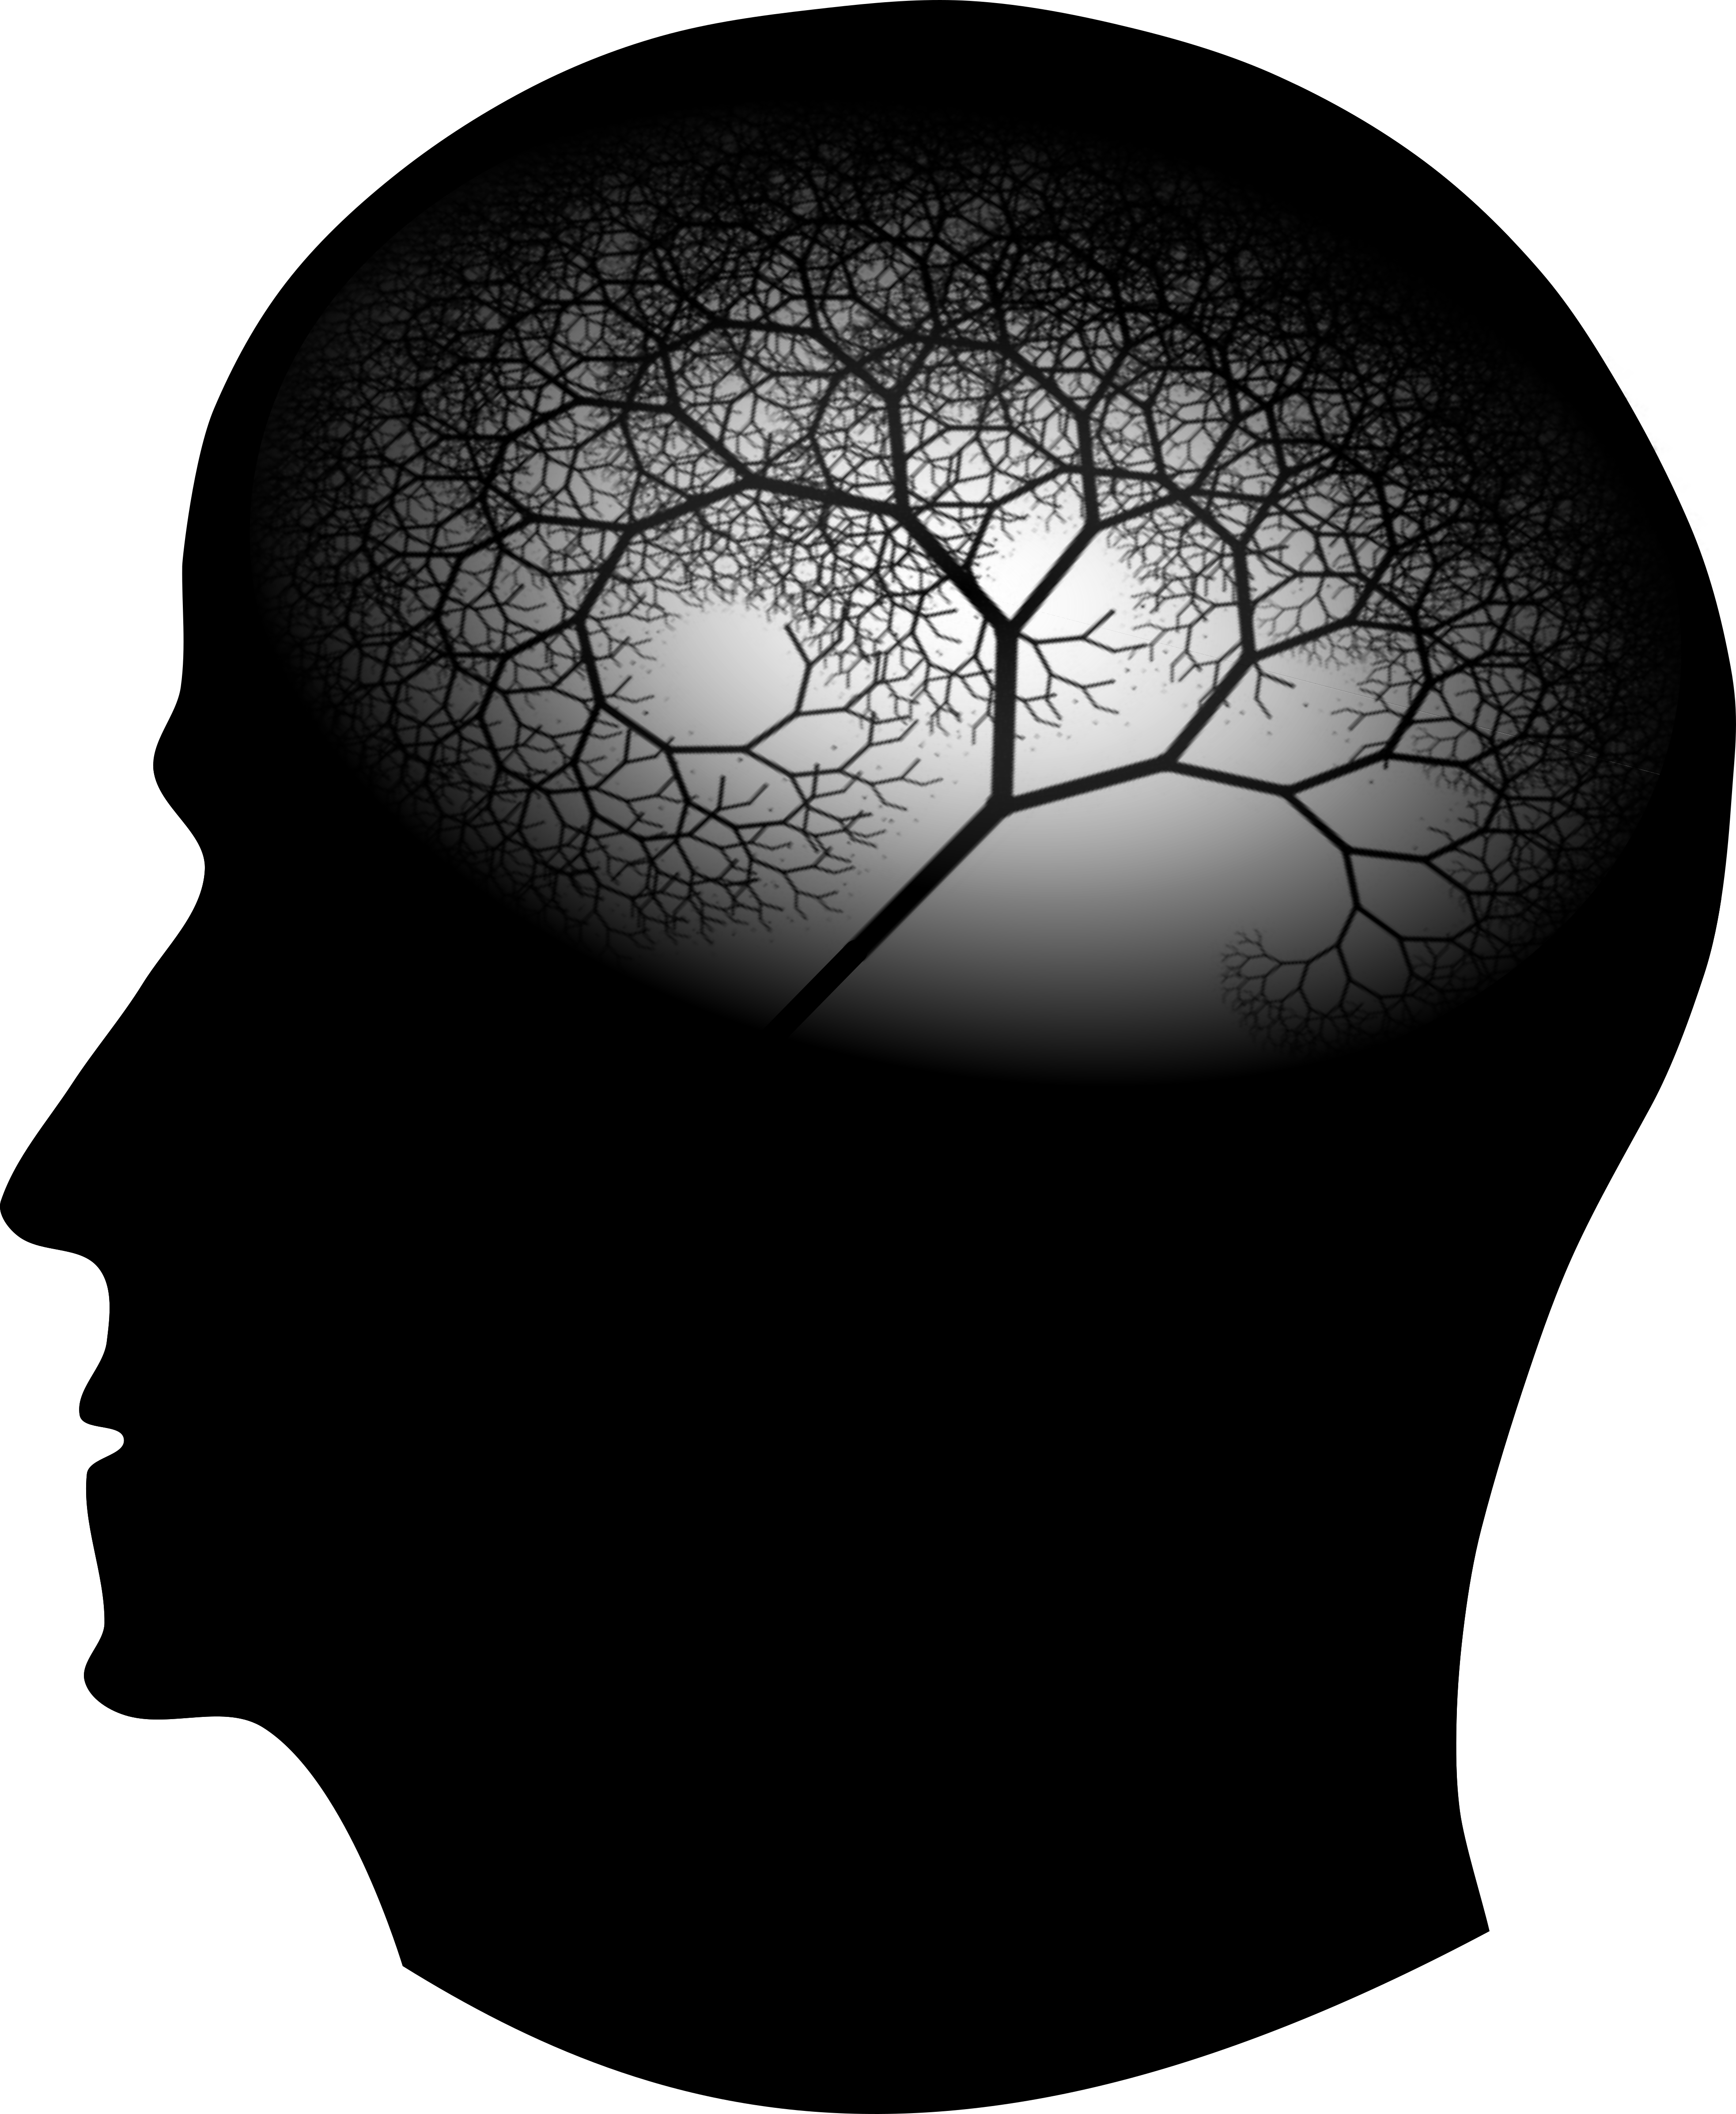
\includegraphics[width = 0.7\textwidth]{frase.png} 
\end{figure*}

\newpage

\setcounter{page}{1}
\pagenumbering{arabic}

%%%%%%%%%%%%%%%%%%%%%%%%%%%%%%%%%%%%%%%%%%%%%%%%%%%%%%%%%%%%%%%%%%%%%%%%%%%%%%%%%%%%%%%%%%%%%%%%%%%
%%%%%%%%%%%%%%%%%%%%%%%%%%%%%%%%%%%%%%%%%%%%%%%%%%%%%%%%%%%%%%%%%%%%%%%%%%%%%%%%%%%%%%%%%%%%%%%%%%%
%%%%%%%%%%%%%%%%%%%%%%%%%%%%%%%%%%%%%%%%%%%%%%%%%%%%%%%%%%%%%%%%%%%%%%%%%%%%%%%%%%%%%%%%%%%%%%%%%%%
%%%%%%%%%%%%%%%%%%%%%%%%%%%%%%%%%%%%%%%%%%%%%%%%%%%%%%%%%%%%%%%%%%%%%%%%%%%%%%%%%%%%%%%%%%%%%%%%%%%

\pagestyle{fancy}
%    \fancyhf{} 
    \fancyhead[LO]{\sectionmark}
    \fancyhead[RE]{\chaptermark}
    \fancyfoot[CE,CO]{}
    \fancyfoot[LE,RO]{\thepage}
    \renewcommand{\headrulewidth}{1.5pt}

%%%%%%%%%%%%%%%%%%%%%%%%%%%%%%%%%%%%%%%%%%%%%%%%%%%%%%%%%%%%%%%%%%%%%%%%%%%%%%%%%%%%%%%%%%%%%%%%%%%
%%%%%%%%%%%%%%%%%%%%%%%%%%%%%%%%%%%%%%%%%%%%%%%%%%%%%%%%%%%%%%%%%%%%%%%%%%%%%%%%%%%%%%%%%%%%%%%%%%%
%%%%%%%%%%%%%%%%%%%%%%%%%%%%%%%%%%%%%%%%%%%%%%%%%%%%%%%%%%%%%%%%%%%%%%%%%%%%%%%%%%%%%%%%%%%%%%%%%%%
%%%%%%%%%%%%%%%%%%%%%%%%%%%%%%%%%%%%%%%%%%%%%%%%%%%%%%%%%%%%%%%%%%%%%%%%%%%%%%%%%%%%%%%%%%%%%%%%%%%

\chapter*{Introducción}
\addcontentsline{toc}{chapter}{Introducción}

Gracias a los avances médicos del último siglo se han incrementado tanto la esperanza como la calidad de vida. 
%
Desafortunadamente, también ha aumentado la presencia de enfermedades no-transmisibles asociadas con la edad. 
%
En México el sector de la población con más de 60 años de edad (considerados en alto riesgo para este tipo de enfermedades) contempló a 10 millones de personas en 2010, y en 2015 dicha cifra creció a 12 millones \cite{Censo10,Intercensal15}.
%
En este trabajo se destaca la demencia entre las enfermedades asociadas con la edad.

La demencia consiste en el desarrollo de deficiencias cognoscitivas (especialmente en atención y memoria) suficientemente graves como para interferir en las actividades del individuo.
%
Hasta el momento se considera que la demencia es irreversible y no se han identificado curas \cite{PlanAlzheimer04}, debido a lo cual ha surgido un gran interés en definir y diagnosticar sus etapas tempranas.
%
El deterioro cognitivo leve (DCL), una etapa temprana de la demencia, se entiende como el desarrollo de deficiencias cognoscitivas \textit{objetivas} que no son lo suficientemente graves para calificarse como demencia.

Existen varios métodos para detectar el DCL, como la autopercepción por parte del paciente, pruebas neuropsicológicas, análisis genéticos, químicos o de imagenología cerebral.
%
Las pruebas neuropsicológicas son usadas en el presente trabajo; se definen como \textit{muestras} de algún comportamiento de interés, obtenidas bajo protocolos estandarizados y calificados de forma objetiva.
%
Debido a la naturaleza parcialmente subjetiva de las pruebas neuropsicológicas, en este trabajo se destaca la técnica de polisomnografía (PSG) que consiste en el registro conjunto de varias señales electrofisiológicas durante el sueño.
%
De manera concreta, será analizada una PSG compuesta por registros de electroencefalografía (EEG), electrooculografía (EOG) y electromiografía (EMG), para medir actividad eléctrica cerebral, tono muscular y movimientos oculares, respectivamente.
%
Se decidió usar la PSG porque es una técnica relativamente barata y no invasiva --en relación al tipo de información que se obtiene--, y porque en la literatura hay una gran cantidad de reportes sobre marcadores para el DCL usando la EEG.

Se han encontrado asociaciones entre el DCL en adultos mayores con la \textit{presencia} de algunos tipos de ondas cerebrales \cite{babiloni13,prichep06,prichep94}.
%
Conviene destacar que se ha indicado que los mejores predictores del DCL son los obtenidos durante el sueño de Movimientos Oculares Rápidos o sueño MOR (a diferencia de la otra gran división del sueño, o No MOR (NMOR)) en comparación con los obtenidos durante la vigilia mediante el uso del análisis espectral \cite{Brayet16}.

%%%%%%%%%%%%%%%%%%%%%%%%%%%%%%%%%%%%%%%%%%%%%%%%%%%%%%%%%%%%%%%%%%%%%%%%%%%%%%%%%%%%%%%%%%%%%%%%%%%
%%%%%%%%%%%%%%%%%%%%%%%%%%%%%%%%%%%%%%%%%%%%%%%%%%%%%%%%%%%%%%%%%%%%%%%%%%%%%%%%%%%%%%%%%%%%%%%%%%%

\section*{Antecedentes}
\addcontentsline{toc}{section}{Antecedentes}

Se considera que la técnica de EEG fue inventada en la década de 1920 por el fisiólogo Hans Berger, quien adicionalmente descubrió que la EEG es \textit{sensible} a algunos cambios en la actividad mental del participante, como estar despierto en reposo y con ojos cerrados, abrirlos o atender de forma sostenida.
%
Desde entonces se estableció que hay una \textit{conexión} entre los fenómenos eléctricos en el cerebro y el funcionamiento de la mente.

Los fenómenos eléctricos en el cerebro que dan origen al EEG se consideran comprendidos en sus \textit{niveles} más básicos: cada neurona genera un potencial eléctrico estable a través de su membrana celular, debido al intercambio de iones con el medio extracelular.
%
Las perturbaciones en estos {potenciales} se trasmiten a través de la membrana, e inducen perturbaciones similares en neuronas cercanas; la morfología de las neuronas permite que formen \textit{redes} para la transmisión de impulsos eléctricos, las cuales se extienden por todo el sistema nervioso.

A partir del mecanismo para la transmisión de impulsos eléctricos, sin embargo, no es muy claro cómo funciona el sistema nervioso central como un todo --o cómo deja de funcionar, como en el caso del DCL.
%
Es necesario considerar que las neuronas no se distribuyen ni forman conexiones de forma aleatoria u homogénea dentro del sistema nervioso, sino que obedecen a un tipo de \textit{organización} que influye en su funcionalidad.
%
Más aún, la existencia de múltiples niveles de organización en la actividad cerebral la han colocado como un \textit{paradigma} de complejidad.

Bajo este contexto se entiende a la complejidad no como complicación, sino como la presencia de características \textit{emergentes}, es decir, que están presentes en un sistema pero no en sus componentes: una neurona individual no exhibe (cualitativamente) el mismo comportamiento eléctrico que todo el cerebro \cite{Werner09}.
%
La complejidad puede describirse informalmente con la frase ``el todo es más que [simplemente] la suma de las partes", entendiendo que la organización es parte de un sistema.

En su célebre libro \textit{``Cybernetics or Control and Communication in the Animal and the Machine"}, el matemático Norbert Wiener propuso que, debido a la gran complejidad de la actividad cerebral, el comportamiento del EEG roza la aleatoriedad; entonces es posible estudiar estos fenómenos usando herramientas de estadística, ignorando parcialmente los procesos físicos y biológicos subyacentes
\cite{wiener61}.
%
Con base a tal comentario, surge históricamente la pregunta sobre hasta qué punto es posible es posible modelar efectivamente al EEG como señales aleatorias con propiedades \textit{simples} e independientes de los complejos procesos subyacentes.
%
Por ejemplo, pueden mencionarse varios trabajos pioneros donde se investiga si los registros de EEG siguen una distribución normal, si son estacionarios, y si su espectro de potencias es \textit{estable} en el tiempo \cite{Cohen77,Kawabata73,McEwen75,Sugimoto78}; en dichos trabajos se demuestra experimentalmente que el EEG puede considerarse estacionario si se usan segmentos de hasta 20 segundos, e incluso se sugiere que esta cantidad puede cambiar para personas con alguna daño neuronal.

Es sumamente interesante el contraste entre la complejidad \textit{innata} del EEG, y la posibilidad de señalar segmentos cuyo comportamiento es relativamente simple.
%
Se ha propuesto que esta característica refleja el comportamiento hipotético de la actividad cerebral como la \textit{orquestación} de múltiples estados de actividad, cada uno con características distintivas, los cuales se alternan entre sí logrando una gran heterogeneidad global \cite{kaplan2000application}.
%
En el caso de la estacionariedad, se usará la formalización para este comportamiento descrita por Dahlhaus, referida como \underline{estacionariedad local} \cite{Dahlhaus97}.

Respecto al supuesto de estacionariedad local en el EEG, cabe destacar que la verificación formal de estacionariedad ha caído en desuso; en cambio, se suelen usar fragmentos de EEG \textit{suficientemente pequeños} para poder suponer estacionariedad \cite{Kaiser00}.
%
Sin embargo, se  ha mostrado que las pruebas de estacionariedad pueden ser útiles, por ejemplo, para segmentar de forma \textit{fisiológicamente relevante} registros de EEG \cite{Kaplan99} y de magnetoencefalografía\footnote{La técnica de magnetoencefalografía (MEG) consiste en el registro de actividad eléctrica del cerebro, a través de perturbaciones en campos magnéticos artificiales.} \cite{lazyref1}, o como apoyo a otras técnicas \cite{allegrini10}.

Bajo el supuesto de estacionariedad local, en el presente trabajo se explora la hipótesis sobre si el DCL afecta a la organización de la actividad cerebral durante el sueño.
%
De manera concreta, se realizaron análisis de estacionariedad en segmentos de PSG de sueño MOR y NMOR para comprobar si hay diferencias entre individuos con y sin DCL.
%
Previamente, se han mostrado resultados que sugieren es posible observar tales cambios
\cite{rosales2017stationarity}.
%\cite{Rosales-Lagarde17}.

Para detectar la estacionariedad se ha usado la prueba descrita por Priestley y Subba Rao \cite{Priestley69}, ya que se ha señalado como una de las más rápidas hasta la fecha \cite{Nason13}, y porque puede ser interpretada de forma relativamente sencilla en términos de un espectro de potencias cambiante en el tiempo. 
%
%Esta última característica es deseable en vista a la gran literatura que existe sobre espectros de potencia para el EEG.

El presente trabajo es un paso en el desarrollo de una metodología para determinar DCL con base en registros de PSG en adultos mayores. En otras palabras, se pretende explorar si es posible encontrar un marcador anatomofisiológico que respalde o complemente los resultados de las pruebas neuropsicológicas.
%
%Se mantiene presente que el deterioro cognitivo (más allá del DCL) no puede reducirse exclusivamente a tales mediciones, y que las conclusiones obtenidas deben ser contrastadas con resultados de análisis complementarios.

%%%%%%%%%%%%%%%%%%%%%%%%%%%%%%%%%%%%%%%%%%%%%%%%%%%%%%%%%%%%%%%%%%%%%%%%%%%%%%%%%%%%%%%%%%%%%%%%%%%
%%%%%%%%%%%%%%%%%%%%%%%%%%%%%%%%%%%%%%%%%%%%%%%%%%%%%%%%%%%%%%%%%%%%%%%%%%%%%%%%%%%%%%%%%%%%%%%%%%%

\section*{Preguntas de investigación y objetivos}
\addcontentsline{toc}{section}{Pregunta de investigación y objetivos}

Se ha supuesto que el fenómeno de estacionariedad local es consecuencia de la complejidad en la actividad eléctrica cerebral, y que ésta última se encuentra asociada a la actividad mental.
%
Los registros de PSG en adultos mayores, modelados como procesos estocásticos, ¿pueden considerarse como débilmente estacionarios? 

Bajo el supuesto de estacionariedad local, ¿la clasificación de estacionariedad débil se ve influida por \textit{parámetros técnicos} como el tamaño de ventana?
%
Con relación a la conexión entre registros de EEG y actividad cerebral, ¿hay diferencias en la clasificación de estacionariedad débil \textit{explicadas} por diferentes estados cognitivos (con o sin DCL) o de actividad cerebral (etapa de sueño NMOR o MOR)?

%%%%%%%%%%%%%%%%%%%%%%%%%%%%%%%%%%%%%%%%%%%%%%%%%%%%%%%%%%%%%%%%%%%%%%%%%%%%%%%%%%%%%%%%%%%%%%%%%%%

\newpage

\subsection*{Objetivos}

%Dar respuesta a las preguntas de investigación 

Para responder a la primera pregunta, se estudiaron algunas pruebas estadísticas para detectar si una realización dada proviene de un proceso estocástico débilmente estacionario; en particular se decidió usar la prueba de Priestley-Subba Rao (PSR).

Para responder las demás preguntas, se usó la prueba de PSR sobre registros de PSG en adultos mayores con y sin Posible DCL (PDCL), diagnosticado usando pruebas neuropsicológicas.
%
En particular, la primera pregunta fue investigada heurísticamente revisando que los resultados fueran \textit{consistentes} para diferentes tamaños de ventana (ningún otro \textit{parámetro técnico} fue investigado).
%
Los resultados obtenidos fueron analizados estadísticamente para revisar la influencia de los factores `\textit{estado mental}' (etapa de sueño) y `estado cognoscitivo' (grupo con o sin PDCL).

%, y revisar qué factores podrían influir en los resultados obtenidos, i.e., el tamaño de la ventana de la señal, clasificación de las señales en MOR o NMOR y características de los participantes.

%

%Por lo tanto, investigar si la cantidad de épocas estacionarias es diferente entre las etapas de sueño MOR y NMOR en distintas ventanas de tiempo.
%
%Estudiar entre las etapas de sueño MOR y NMOR, si hay una relación entre la presencia de PDCL y la clasificación de los procesos estocásticos referidos como débilmente estacionarios.


\section*{Acerca de la estructura del texto}

Debido al enfoque \textit{aplicado} del presente trabajo, el primer objetivo se satisface en los dos primeros capítulos y los dos primeros apéndices.
%
El primer capítulo se exponen varios temas preliminares, con el fin de lograr un texto autocontenido y accesible; este capítulo se complementa con el apéndice A, donde se presenta el sustento formal de varios objetos usados durante el texto pero que pueden omitirse.
%
%Entre los temas más importantes se encuentran procesos estocásticos, estacionariedad débil, estimadores, pruebas de hipótesis.

%El primer capítulo se incluye con la finalidad de lograr un texto autocontenido, y en él se exponen una serie de temas preliminares aunque sin gran detalle.
%%
%Entre los temas más importantes se encuentran procesos estocásticos, estacionariedad débil, estimadores, pruebas de hipótesis.

En el segundo capítulo se expone la herramienta principal del presente trabajo: la prueba de estacionariedad débil de PSR.
%
Este objeto exige la exposición previa del \textit{espectro evolutivo} y de un estimador para éste, ya que representan la base formal de la prueba.
%
Para mantener el enfoque del texto, las demostraciones formales sobre las propiedades de estos objetos son relegadas al apéndice B.

%En el segundo capítulo el tema principal es el espectro de evolutivo y estacionariedad  débil; adicionalmente se discute sobre su estimación.
%Al final se expone una aplicación aparente menor del espectro evolutivo, pero que es fundamental para el resto del presente trabajo: la prueba de Priestley Subba-Rao. 

%Esta prueba verifica --como prueba de hipótesis-- si el espectro evolutivo de un proceso puede reducirse a un espectro de potencias; en otras palabras, si un proceso es débilmente estacionario.

Se incluye en el tercer capítulo una se expone brevemente los temas \textit{necesarios} para entender el DCL y la PSG. 
%
Se describe qué es el DCL y cómo se detecta, qué es el sueño y cómo se analiza (en particular usando la PSG), y se menciona la relación entre el sueño y el DCL.

%El objetivo del tercer capítulo es describir el DCL y cómo se detecta, qué es el sueño y cómo se analiza (en particular usando la PSG), y mencionar la relación entre el sueño y el DCL.
%%
%Para ello se presentan algunos conceptos de psicología, psicometría, fisiología y electrofisiología.

Se responde a las últimas dos preguntas de investigación en el capítulo cuarto y quinto, exponiendo los resultados obtenidos y las conclusiones.

Se concluye que es que la metodología descrita pueda constituirse como un marcador diagnóstico del PDCL, y que quizá pueda usarse como base para construir marcadores diagnósticos para el DCL.

%En el capítulo cuarto se describe cómo se utilizó la prueba de estacionariedad débil para estudiar los registros de polisomnografía.
%%
%En el capítulo quinto se discuten los resultados obtenidos, y se concluye que la técnica utilizada es un marcador diagnóstico para el DCL; se reportan algunos hallazgos incidentales.

%\begin{figure}
%\centering
%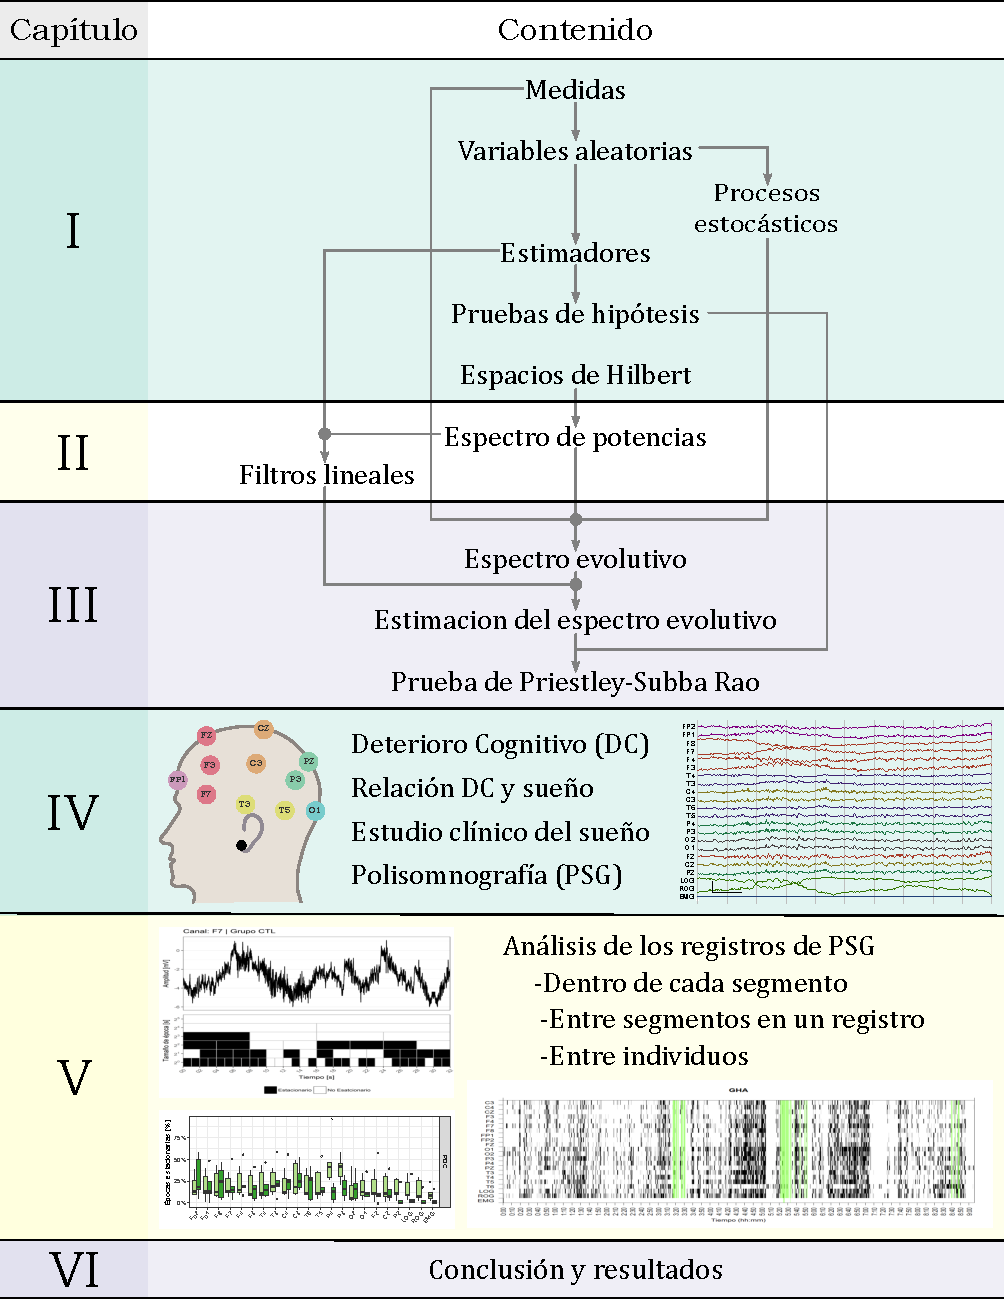
\includegraphics[width=.9\textwidth]{./estructura_texto_v2.pdf}
%\caption[Estructura de la tesis]{Se ilustran gráficamente las \textit{dependencias} respecto a los tópicos de matemáticas, es decir, los temas que deben discutirse antes que otros. Los capítulos 1,2 y 3 se reducen al capítulo 1 y 2,  y los detalles que se ilustran en la figura se encuentran en el apéndice. El resto del texto (incluyendo los tópicos de fisiología) son expuestos de forma más \textit{secuencial}, por lo que no se consideró necesario ilustrar sus dependencias.}
%\label{intro:estructura}
%\end{figure}

%%%%%%%%%%%%%%%%%%%%%%%%%%%%%%%%%%%%%%%%%%%%%%%%%%%%%%%%%%%%%%%%%%%%%%%%%%%%%%%%%%%%%%%%%%%%%%%%%%%
%%%%%%%%%%%%%%%%%%%%%%%%%%%%%%%%%%%%%%%%%%%%%%%%%%%%%%%%%%%%%%%%%%%%%%%%%%%%%%%%%%%%%%%%%%%%%%%%%%%
%%%%%%%%%%%%%%%%%%%%%%%%%%%%%%%%%%%%%%%%%%%%%%%%%%%%%%%%%%%%%%%%%%%%%%%%%%%%%%%%%%%%%%%%%%%%%%%%%%%
%%%%%%%%%%%%%%%%%%%%%%%%%%%%%%%%%%%%%%%%%%%%%%%%%%%%%%%%%%%%%%%%%%%%%%%%%%%%%%%%%%%%%%%%%%%%%%%%%%%

\chapter{Preliminares}

En este capítulo se exponen varios temas que, en lo posterior, serán considerados como \textit{conocidos} y usados extensamente.
%
Con el fin de lograr un texto autocontenido y accesible, se incluye en el apéndice \ref{apendice:medidas} una discusión más detallada sobre estos tópicos.
%
El lector interesado en una profundización aún mayor sobre teoría de la medida, probabilidad y estadística puede referirse a los libros \textit{``Probability for Statisticians"} por Galen R. Shorack \cite{probabilidad_shorack}, y \textit{``Statistical Theory"} por Bernard W. Lindgren \cite{estadistica_lindgren}.

%%%%%%%%%%%%%%%%%%%%%%%%%%%%%%%%%%%%%%%%%%%%%%%%%%%%%%%%%%%%%%%%%%%%%%%%%%%%%%%%%%%%%%%%%%%%%%%%%%%
%%%%%%%%%%%%%%%%%%%%%%%%%%%%%%%%%%%%%%%%%%%%%%%%%%%%%%%%%%%%%%%%%%%%%%%%%%%%%%%%%%%%%%%%%%%%%%%%%%%

\section{Procesos estocásticos}

Los procesos estocásticos se definen formalmente como variables aleatorias cuyo espacio muestral es un espacio de funciones.
%
Intuitivamente es posible definir los procesos estocásticos como una \textit{concatenación} de variables aleatorias, es decir, un conjunto de variables aleatorias indexadas sobre algún conjunto arbitrario.
%
Sin embargo, indexar un conjunto infinito de variables aleatorias representa un problema técnico en el cuanto a definir al proceso estocástico como espacio de probabilidad, especialmente al definir la medida de probabilidad asociada.

Debido a las limitaciones del presente trabajo, el tema se expone de manera parcial bajo un enfoque formal; la exposición se basa en aquella presentada por Kolmogorov \cite{kolmogorov2018foundations}, de modo que el lector interesado debe dirigirse a dicho texto.

Primeramente se define a $\R^{\mathcal{T}}$, el conjunto de funciones con dominio en $\mathcal{T}$ y codominio en $\R$, el cual será usado como espacio de eventos\footnote{Se puede definir análogamente a $\C^{\mathcal{T}}$, o espacios más generales}. 
%
A modo de \textit{intervalos generalizados} se definen los conjuntos de la forma
\begin{equation}
I\left( [t_1, a_1, b_1], \cdots, [t_N, a_N, b_N] \right) = 
\left\{ f \in \R^{\mathcal{T}} \talque f(t_i) \in (a_i, b_i] \, , \, i = 1, \cdots, N \right\}
\end{equation}

Es relativamente fácil extender la familia de estos intervalos por uniones e intersecciones finitas. %
Es un tanto más interesante definir una $\sigma$-álgebra generada por éstos conjuntos, pero tal parte se omite en el presente trabajo.
%
En el texto por Kolmogorov se explora con mayor detalle la existencia de dicha $\sigma$-álgebra --y por tanto, la existencia de procesos estocásticos.

\begin{definicion}
Un \textbf{proceso estocástico} \xt es una colección de variables aleatorias indexadas por el símbolo $t\in\mathcal{T}$.
\end{definicion}

\begin{definicion}
Se dice que un proceso estocástico \xt es un \textbf{proceso estocástico en $\R$} si cumple que $\mathcal{T} \subseteq \R$.
%
Por notación, el índice $t$ es referido como \textbf{tiempo}, mientras que $\mathcal{T}$ es el conjunto de \textbf{tiempos admisibles}.
\end{definicion}

Por simplicidad, durante el presente trabajo sólo se usarán dos familias de procesos estocásticos en $\R$: si $\mathcal{T}$ es un intervalo, o si es parte de una \textit{malla}. 
%
La primera familia se reserva para modelar las señales electrofisiológicas, mientras que la segunda se usará para modelar los registros de estas mismas señales.
%
La distinción consiste en que las señales electrofisiológicas sólo pueden ser registradas digitalmente en un conjunto finito de puntos en el tiempo; la atención del texto recae en ambos grupos de procesos, en espera que sus características sean similares de algún modo.

\begin{definicion}
Se dice que un proceso estocástico en $\R$ es \textbf{a tiempo continuo} si existen $a, b \in \R \cup \{ -\infty, \infty \}$ tales que
\begin{equation}
\mathcal{T} = (a,b)
\end{equation}
Así mismo, se dice que un proceso estocástico en $\R$ es \textbf{a tiempo discreto} si existen $t_0, \Delta_X \in \R \cup \{ -\infty, \infty \}$ tales que
\begin{equation}
\mathcal{T} = \left\{ t_0 + t \in \R \talque {t} \cdot {\Delta_X} \in \Z \right\}
\end{equation}
Por notación, $\Delta_X$ es referida como \textit{frecuencia de muestreo}.
\end{definicion}

Conviene destacar que el nombre \textit{frecuencia de muestreo} hace referencia al proceso de registro, que algunos textos es referido como \textit{muestreo}; esta terminología entra claramente en conflicto con las muestras de una variable aleatoria. En lo siguiente se evita llamar muestreo al proceso de registro, pero se conservará el término frecuencia de muestro.

Cabe mencionar que hay un conflicto similar con los términos \textit{tiempo continuo} y \textit{tiempo discreto}; estos términos \underline{no guardan ninguna analogía} con las variables aleatorias discretas y continuas, ni con los espectro de potencias puramente continuos o puramente discretos (ver el capítulo siguiente).
%
Estos términos se usan porque se encuentran muy extendidos en la literatura sobre análisis de señales.

Para facilitar la referencia de procesos estocásticos, los elementos que lo componen son denotados como:
\begin{description}
\item[\xt]        Todo el proceso.
\item[$X(t)$]     Variable aleatoria en el proceso, para el tiempo $t \in \mathcal{T}$.
\item[$x(t)$]     Una observación de $X(t)$, para el tiempo $t \in \mathcal{T}$.
\item[$F_{X(t)}$] Función de probabilidad acumulada para $X(t)$.
\end{description}

%%%%%%%%%%%%%%%%%%%%%%%%%%%%%%%%%%%%%%%%%%%%%%%%%%%%%%%%%%%%%%%%%%%%%%%%%%%%%%%%%%%%%%%%%%%%%%%%%%%
%%%%%%%%%%%%%%%%%%%%%%%%%%%%%%%%%%%%%%%%%%%%%%%%%%%%%%%%%%%%%%%%%%%%%%%%%%%%%%%%%%%%%%%%%%%%%%%%%%%

\subsection{Estacionariedad débil}

De forma general, la estacionariedad significa que \textit{algunas} propiedades de un proceso sean \textit{invariantes} en el tiempo; la decisión sobre cuáles son estas características lleva a diferentes definiciones de estacionariedad.
%
Se decidió conveniente usar la definición \ref{est_m} con $m=2$, ya que garantiza que los momentos conjuntos de orden 2 son constantes en el tiempo y por tanto pueden ser estimadas.
%
La motivación principal para ello es la siguiente: si se modela una señal como proceso estocástico, entonces los momentos están asociados con variables físicas relevantes; en particular, el segundo momento está asociado con la \textit{energía} (definición \ref{lazy5}).

\begin{definicion}%[Estacionariedad de orden $m$]
\label{est_m}
Un proceso \xt se dice \textbf{estacionario de orden $\boldsymbol{m}$} si, para cualesquiera $t_1, t_2, \dots, t_n \in \mathcal{T}$ y cualquier $\tau$ tal que $t_i + \tau \in \mathcal{T}$, se cumple que
\begin{equation}
\E{X^{m_1}(t_1)X^{m_2}(t_2)\cdots X^{m_n}(t_n)} =
\E{X^{m_1}(t_1+\tau)X^{m_2}(t_2+\tau)\cdots X^{m_n}(t_n+\tau)}
\end{equation}
para cualesquiera enteros $m_1, m_2, \dots, m_n$ tales que $m_1+m_2+\cdots+m_n \leq m$.
\end{definicion}

\begin{definicion}
\label{lazy5}
Sean $[a,b] \subseteq \R$ un intervalo arbitrario, y sea $f: [a,b] \rightarrow \R$ una función integrable. La \textbf{energía disipada} por la función $f$ en el intervalo de tiempo $[a,b]$ es
\begin{equation}
\text{energía}_{[a,b]}[f] = \int_a^{b} \abso{f(t)}^{2} dt
\end{equation}
%Similarmente, la \textbf{potencia} de la función $f$ en el intervalo de tiempo $[a,b]$ es
%\begin{equation}
%\text{potencia}_{[a,b]}[f] = \frac{1}{b-a} \int_a^{b} \abso{f(t)}^{2} dt
%\end{equation}
\end{definicion}

La definición \ref{est_m} es conveniente también porque, para analizar la energía de un proceso, se requieren poner condiciones adicionales; por ejemplo, para estimar la varianza de un estimador para la energía, se requiere que el proceso sea estacionario de orden 4.
%
Bajo los términos de esta definición se puede decir que, por motivos meramente fisiológicos, las señales electrofisiológicas siempre estacionarias de orden 1.

En otro sentido, usar la estacionariedad de orden 2 permite calcular las covarianzas de forma sencilla. 
%
Con base a lo anterior, es común usar la \underline{estacionariedad débil}, una definición equivalente pero más extendida.

\begin{definicion}%[Estacionariedad débil]
Un proceso \xt se dice \textbf{débilmente estacionario} si existe $\mu \in \R$ y una función $R^\star : \mathcal{T} \rightarrow \R $ tales que, para cualesquiera $t, s \in T$ se 
cumple
\begin{itemize}
\item $\E{X(t)} = \mu$
%\item $\Var{X(t)} = \sigma^{2}$
\item $\Cov{X(t),X(s)} = R^\star(\abso{s-t})$
\end{itemize}
\end{definicion}

\begin{proposicion}
Para que un proceso estocástico \xt sea débilmente estacionario es suficiente y necesario que sea estacionario de orden 2.
\end{proposicion}

El que un proceso sea débilmente estacionario implica la existencia de una función referida como \textit{función de autocovarianza}.
%
Se puede definir una versión generalizada de esta función para cualquier proceso estocástico, entendiendo que adopta \textit{cierta forma} cuando el proceso es débilmente estacionario.

\begin{definicion}
Sea \xt un proceso estocástico en los reales. Su \textbf{núcleo de covarianza} se define, para cualesquiera tiempos admisibles $t,s\in\mathcal{T}$, como
\begin{equation}
R(s,t) := \E{{\left( X(t)-\E{X(t)} \right)}\left( X(s)-\E{X(s)} \right)}
\end{equation}
\end{definicion}

%Como las señales electrofisiológicas son modeladas como procesos estocásticos, conviene traducir algunas de sus características en propiedades para los procesos estocásticos.
%%
%Por ejemplo, se sabe que las señales representan variaciones en campos eléctricos, y entonces se puede afirmar sin duda que dicha cantidad es finita en todo momento; lo mismo se puede afirmar sobre la energía.
%%
%En base a ello, los procesos estocásticos que modelan señales electrofisiológicas deben tener energía y varianza finitas en todo momento.
%%
%Más aún, la actividad eléctrica cerebral y muscular presentan durante el reposo una actividad característica, referida como \textit{actividad basal} o \textit{línea base}, que es relativamente cercana a una constante en todo momento (ver figura \ref{ejemplos_mor}).
%%
%El fenómeno de línea base entra en el modelado como el supuesto de que las señales son procesos estacionarias de orden 1; por simplicidad, se puede considerar que la media de estos procesos es 0.

\subsection{Ejemplos}

\begin{ejemplo}
Un \underline{proceso oscilante} es un proceso estocástico $\{ S(t)\}_{t\in\R}$ definido como
\begin{equation}
S(t) = \COS{t + \phi}
\end{equation}
donde $\phi \sim \text{unif}(-\pi,\pi)$.
%
Es muy notable que el proceso esté \textit{caracterizado} por una única variable aleatoria y que sus realizaciones siempre son funciones \textit{suaves}, contrario al estereotipo para estas funciones.

Su valor esperado puede ser calculado fácilmente
\begin{align}
\E{S(t)} &= \E{\COS{t + \phi}} = \frac{1}{2 \pi} \int_{-\pi}^\pi \COS{t + \phi} d\phi = 0
\end{align}

Similarmente para la función de autocovarianza
\begin{align}
\E{S(t)S(s)} &= 
\E{\COS{t + \phi}\COS{s + \phi}} \nonumber \\
&=
\E{\frac{1}{2} \COS{t-s} + \frac{1}{2}\COS{t+s+2\phi}} \nonumber \\
&=
\frac{1}{2} \COS{t-s} + \frac{1}{2} \E{\COS{t+s+2\phi}} \nonumber \\
&= \frac{1}{2} \COS{t-s}
\end{align}

Se concluye que $\{ S(t)\}_{t\in\R}$ es débilmente estacionario.
%
Un segundo aspecto notorio en este ejemplo es que la función de autocovarianza es periódica, contrario al estereotipo de que las funciones autocorrelación siempre decaen exponencialmente.
\end{ejemplo}

\begin{ejemplo}
Un \underline{proceso ruido blanco} es un proceso estocástico $\{ \varepsilon(t)\}_{t\in\R}$ tal que si $t, s\in \R$ son diferentes entonces $\varepsilon(t)$ y $\varepsilon(s)$ son indepentiendes.
%
Se dice que el proceso ruido blanco es `normal' si $\varepsilon(t) \sim N(0,1)$.
%$\varepsilon(t) \sim N(0,\sigma^2)$ para algún $\sigma\in\R$. 
%
Por simplicidad, el término ruido blanco será usado de forma general para procesos normales estándar, con el fin de garantizar que son débilmente estacionarios.

La función de autocovarianza de un proceso ruido blanco es
\begin{equation}
R(\tau) = \begin{cases}
1 &, \tau = 0 \\
0 &, \text{otro caso}
\end{cases}
\end{equation}
Se concluye que el proceso ruido blanco es débilmente estacionario, pero no es estocásticamente continuo.
\end{ejemplo}

\begin{figure}
\centering
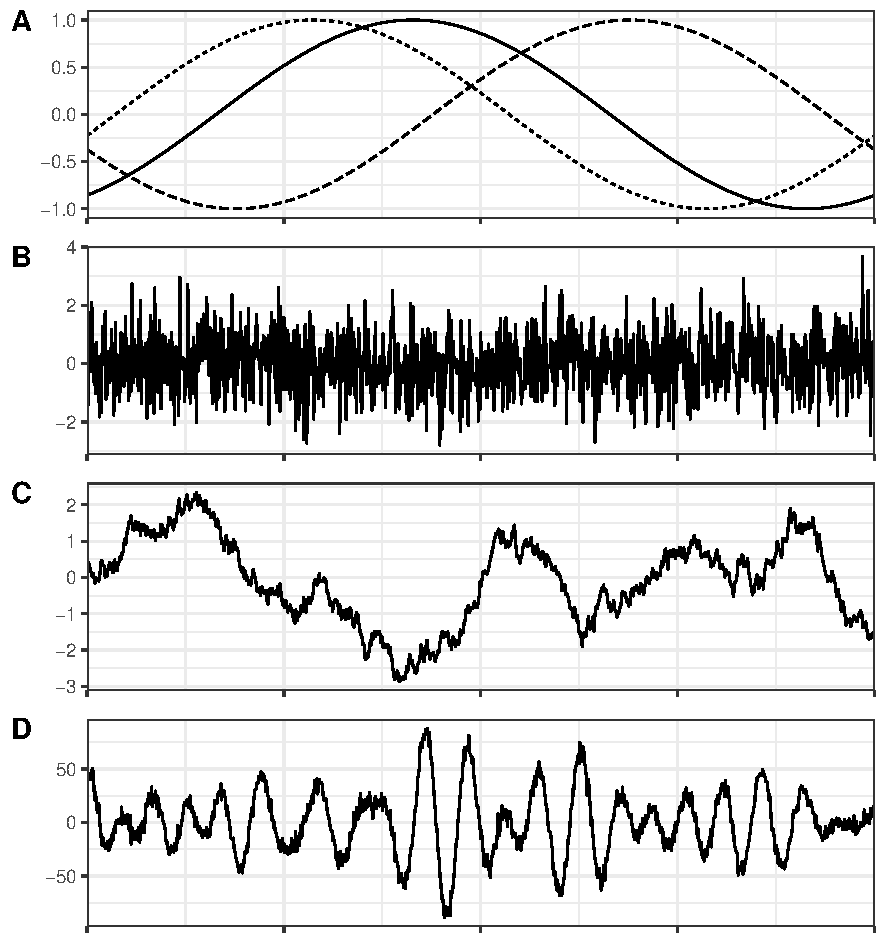
\includegraphics[width=\linewidth]{./img_mas_ejemplos/ruidos_ejemplos.pdf}
\caption[Ejemplos de procesos estocásticos.]{Ejemplos de realizaciones para algunos procesos estocásticos. \textbf{A.} Proceso oscilante, del cual se grafican tres realizaciones diferentes. \textbf{B.} Proceso Ruido Blanco. \textbf{C.} Proceso de Wiener. \textbf{D.} Proceso medias móviles a tiempo continuo con parámetro $A=\nicefrac{1}{4}$.}
\end{figure}

%%%%%%%%%%%%%%%%%%%%%%%%%%%%%%%%%%%%%%%%%%%%%%%%%%%%%%%%%%%%%%%%%%%%%%%%%%%%%%%%%%%%%%%%%%%%%%%%%%%
%%%%%%%%%%%%%%%%%%%%%%%%%%%%%%%%%%%%%%%%%%%%%%%%%%%%%%%%%%%%%%%%%%%%%%%%%%%%%%%%%%%%%%%%%%%%%%%%%%%

%\subsection{Integración y procesos estocásticos}
%\label{sec:int_proc_est}
%
%La integral, según las definiciones \ref{def:lazy1} y \ref{def:lazy2}, puede extenderse intuitivamente respecto a un proceso estocástico.
%%
%Este tema no será explorado con mayor detalle en el presente texto, sino que sólo será usado para construir algunos ejemplos.
%%
%Para ello se define al proceso de Wiener, un proceso estocástico con algunas propiedades peculiares que serán de gran utilidad.
%
%\begin{ejemplo}
%Un \underline{proceso de Wiener} es un proceso estocástico $\{ W(t)\}_{t\in\R}$ que satisface las siguientes propiedades para cualesquiera $t, s, \in \R$
%\begin{itemize}
%\item $W(0) \sim \text{D}(0)$
%\item $\left[W(t)-W(s)\right] \sim N(0, \abso{t-s})$
%\item $\left[W(t)-W(s)\right]$ es independiente de $W(u)$ para $u < \min\{ t, s \}$
%\end{itemize}
%
%Es relativamente fácil notar que $\E{W(t)} = 0$ y $\E{\left(W(t)\right)^2}$, de donde se deduce que el proceso de Wiener no es débilmente estacionario.
%\end{ejemplo}
%
%Así entonces, sea $\{ W(t)\}_{t\in\R}$ un proceso de Wiener, $[a,b]\subseteq\R$ un intervalo arbitrario, y $f:[a,b]\longrightarrow\R_+$ una función medible.
%%
%Sean $t_1, t_2, \dots, t_N \in \R$ una partición arbitraria de $[a,b]$, es decir que satisfacen
%\begin{equation}
%a < t_1 < t_2 < \dots < t_N < b
%\end{equation}
%entonces se define la variable aleatoria
%\begin{equation}
%\sum_{i=2}^N \left[ \sup_{\lambda \in [t_{i-1},t_i]} f(\lambda) \right] \left[ W(t_i) - W(t_{i-1}] \right)
%\end{equation}
%
%\underline{Si} la colección de variables aleatorias converge en media cuadrática entonces se dice que
%\begin{equation}
%\int_a^b f(t) dW(t) :=
%\lim_{N\rightarrow \infty} \left(
%\sum_{i=2}^N \left[ \sup_{\lambda \in [t_{i-1},t_i]} f(\lambda) \right] \left[ W(t_i) - W(t_{i-1}] \right] \right)
%\end{equation}
%
%\begin{proposicion}
%Sea $\{ W(t)\}_{t\in\R}$ un proceso de Wiener, $[a,b]\subseteq\R$ un intervalo arbitrario, y $f:[a,b]\longrightarrow\R_+$ una función medible. Entonces
%\begin{equation}
%\E{\int_a^b f(t) dW(t) } = 0
%\end{equation}
%\label{prop:lazy000}
%\end{proposicion}
%\begin{proof}
%Sea $\Delta W_i = W(t_i) - W(t_{i-1})$, el cual satisface las siguientes propiedades
%\begin{itemize}
%\item $\E{\Delta W_i} = 0$
%\item $\E{\left( \Delta W_i \right)^2} = t_{i} - t_{i-1}$
%\item Si $i<j$ entonces $\Delta W_i$ y $\Delta W_j$ son independientes
%\end{itemize} 
%
%Entonces, nótese que
%\begin{align*}
%\E{\int_a^b f(t) dW(t) } &=
%\E{ \lim_{N\rightarrow \infty} \left( \sum_{i=2}^N f_i \Delta W_i \right) } \\
%&= 
%\lim_{N\rightarrow \infty} \left( \sum_{i=2}^N f_i \E{ \Delta W_i } \right) \\
%&= 0
%\end{align*}
%donde $f_i = \sup_{\lambda \in [t_{i-1},t_i]} f(\lambda)$.
%\end{proof}
%
%\begin{proposicion}
%Sea $\{ W(t)\}_{t\in\R}$ un proceso de Wiener, $[a,b]\subseteq\R$ un intervalo arbitrario, y $f:[a,b]\longrightarrow\R_+$ una función medible. Entonces
%\begin{equation}
%\E{\left(\int_a^b f(t) dW(t) \right)^2 } = \int_a^b \left[ f(t) \right]^2 dt
%\end{equation}
%\label{prop:lazy100}
%\end{proposicion}
%\begin{proof}
%Sea $\Delta W_i = W(t_i) - W(t_{i-1})$, como en la demostración anterior.
%Nótese que
%\begin{align*}
%\E{\left(\int_a^b f(t) dW(t) \right)^2 } &=
%\E{\left( \lim_{N\rightarrow \infty} \left(
%\sum_{i=2}^N f_i \Delta W_i \right) \right)^2} \\
%&= 
%\lim_{N\rightarrow \infty} \E{ \left(
%\sum_{i=2}^N f_i \Delta W_i \right)^2} \\
%&=
%\lim_{N\rightarrow \infty} \sum_{i=2}^N \sum_{j=2}^N
%f_i f_j \E{  \Delta W_i \Delta W_j } \\
%&=
%\lim_{N\rightarrow \infty} \sum_{i=2}^N
%f_i^2 \E{  \left( \Delta W_i \right)^2 } \\
%&=
%\lim_{N\rightarrow \infty} \sum_{i=2}^N
%f_i^2 (t_i-t_{i-1}) \\
%&=
%\int_a^b \left[ f(t) \right]^2 dt
%\end{align*}
%donde $f_i = \sup_{\lambda \in [t_{i-1},t_i]} f(\lambda)$.
%\end{proof}
%
%\begin{ejemplo}
%Sea $\{ W(t)\}_{t\in\R}$ un proceso de Wiener y sea $A\in\R_+$ arbitrario. Se define a $\{Y(t)\}_{t\in\R}$, un \underline{proceso medias m\'oviles tiempo continuo} con parámetro $A$, como
%\begin{equation}
%Y(t) = \frac{1}{A}\int_{t-\nicefrac{A}{2}}^{t+\nicefrac{A}{2}} dW(u)
%\end{equation}
%
%Con base a la proposición \ref{prop:lazy000}, se deduce que
%\begin{equation}
%\E{Y(t)} = 0
%\end{equation}
%Así mismo, usando la proposición \ref{prop:lazy100} se deduce la función de autocovarianza
%\begin{align*}
%\E{Y(t)Y(s)} &= 
%\E{ \left( \frac{1}{A}\int_{\Omega_t} dW(u) \right) \left( \frac{1}{A}\int_{\Omega_s} dW(v)\right) } \\
%&= 
%\frac{1}{A^2} 
%\E{ 
%\left( 
%\int_{\Omega_t \cap \Omega_s^C} dW(u) + \int_{\Omega_t \cap \Omega_s} dW(u) 
%\right)
%\left( 
%\int_{\Omega_s \cap \Omega_t^C} dW(v) + \int_{\Omega_t \cap \Omega_s} dW(v) 
%\right)  
%} \\
%&=
%\frac{1}{A^2} 
%\E{  
%\int_{\Omega_t \cap \Omega_s^C} dW(u)  
%}
%\E{
%\int_{\Omega_s \cap \Omega_t^C} dW(v) 
%} \\
%&\pheq
%+ \frac{1}{A^2} 
%\E{ 
%\int_{\Omega_t \cap \Omega_s^C} dW(u)  
%}
%\E{
% \int_{\Omega_t \cap \Omega_s} dW(v) 
%} \\
%&\pheq
%+\frac{1}{A^2} 
%\E{ 
%\int_{\Omega_t \cap \Omega_s} dW(u) 
%}
%\E{
%\int_{\Omega_s \cap \Omega_t^C} dW(v)
%} \\
%&\pheq
%+\frac{1}{A^2} 
%\E{ 
%\left( 
%\int_{\Omega_t \cap \Omega_s} dW(u) 
%\right)^2
%} \\
%&= \frac{1}{A^2} \max \{ A-\abso{t-s}, 0 \}
%\end{align*}
%donde $\Omega_t = \left[ t - \nicefrac{A}{2}, t + \nicefrac{A}{2} \right]$ y similarmente para $\Omega_s$.
%%
%En particular, el proceso de medias móviles a tiempo continuo es débilmente estacionario.
%%
%Por simplicidad, este proceso será referido simplemente como \textit{proceso medias móviles}.
%\end{ejemplo}

%
%\begin{figure}
%\centering
%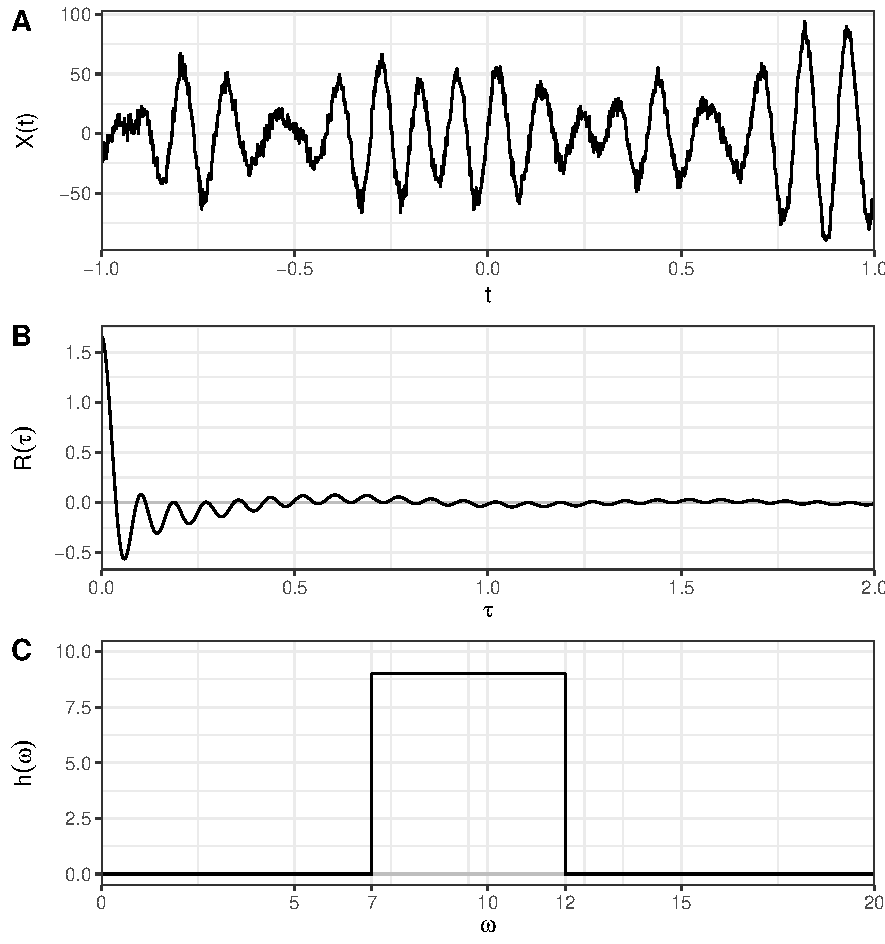
\includegraphics[width=\linewidth]{./img_mas_ejemplos/proceso_alfa.pdf}
%\caption[Apariencia del proceso tipo alfa]{Apariencia del proceso tipo alfa, descrito en el ejemplo \ref{lazy:proceso_alfa}. \textbf{A.} Una realización del proceso, $H$, construida a partir de una realización del proceso ruido blanco. \textbf{B.} Función de autocorrelación, $R$, construida analíticamente. \textbf{C.} Función de densidad espectral, $h$, construida analíticamente.}
%\label{img:proceso_alfa}
%\end{figure}

%\begin{ejemplo}
%Sea $\{Y(t)\}_{t\in \mathcal{T}}$ un proceso de estocástico en $\R$, débilmente estacionario, cuya función de autocorrelación es\footnote{Un proceso así puede ser construido usando \textit{filtros lineales}, tal como son expuestos en la sección \ref{sec:lazy_filtros}.}
%\begin{equation}
%R(t) = \frac{\SEN{10 \pi t}}{t} - \frac{\SEN{7 \pi t}}{t}
%\end{equation}
%
%Este proceso será referido como \underline{proceso tipo alfa} y usado en ejemplos posteriores; el nombre se debe a la analogía con las ondas cerebrales alfa, como se describen en la sección \ref{sec:eeg}.
%%
%En la figura \ref{img:proceso_alfa} se ilustra la apariencia de este proceso, su función de covarianza y su función de densidad espectral.
%\label{lazy:proceso_alfa}
%\end{ejemplo}

\begin{ejemplo}
Un \underline{proceso de Wiener} es un proceso estocástico $\{ W(t)\}_{t\in\R}$ que satisface las siguientes propiedades para cualesquiera $t, s, \in \R$
\begin{itemize}
\item $W(0) \sim \text{D}(0)$
\item $\left[W(t)-W(s)\right] \sim N(0, \abso{t-s})$
\item $\left[W(t)-W(s)\right]$ es independiente de $W(u)$ para $u < \min\{ t, s \}$
\end{itemize}

Es relativamente fácil notar que $\E{W(t)} = 0$ y $\Cov{W(t),W(s)} = \min\{t,s\}$, de donde se deduce que el proceso de Wiener no es débilmente estacionario.
\end{ejemplo}

\begin{ejemplo}
\label{ejemplo:ma}
Sea $\{ W(t)\}_{t\in\R}$ un proceso de Wiener y sea $A\in\R_+$ arbitrario. Se define a $\{Y(t)\}_{t\in\R}$, un \underline{proceso medias m\'oviles tiempo continuo} con parámetro $A$, como
\begin{equation}
Y(t) = \frac{1}{A}\int_{t-\nicefrac{A}{2}}^{t+\nicefrac{A}{2}} dW(u)
\end{equation}
En la sección \ref{sec:int_proc_est} se demuestra que el proceso está bien definido, y además que su función de autocovarianza es
\begin{equation}
R(\tau) = \frac{1}{A^2}\min\{ A - \abso{\tau} , 0 \}
\end{equation}
\end{ejemplo}

%%%%%%%%%%%%%%%%%%%%%%%%%%%%%%%%%%%%%%%%%%%%%%%%%%%%%%%%%%%%%%%%%%%%%%%%%%%%%%%%%%%%%%%%%%%%%%%%%%%
%%%%%%%%%%%%%%%%%%%%%%%%%%%%%%%%%%%%%%%%%%%%%%%%%%%%%%%%%%%%%%%%%%%%%%%%%%%%%%%%%%%%%%%%%%%%%%%%%%%

\section{Estimación de parámetros}

Hasta ahora se ha hablado de las variables aleatorias y procesos estocásticos únicamente como objetos definidos formalmente.
%
En el contexto del presente trabajo, dichos objetos son usados para modelar fenómenos físicos, es decir que se espera que ciertos fenómenos presenten comportamientos similares a cierto tipo de variables aleatorias.
%
En esta sección se aborda el problema formal de \textit{recuperar} información sobre estos objetos en base a las observaciones obtenidas del fenómeno estudiado, las cuales son interpretadas como \textit{huellas} de estos objetos aleatorios.

Considérese a $X$, una variable aleatoria entre los espacios medibles $(\Omega_1,\mathcal{U}_1)$ y $(\Omega_2,\mathcal{U}_2)$. 
%
Para poder \textit{conectar} a $X$ con el fenómeno estudiado, $\Omega_1$ debe incluir todas los estados posibles del sistema bajo las condiciones de estudio; mientras, $\Omega_2$ es típicamente un conjunto \textit{basado} en $\R$ suficientemente general para cuantificar \textit{adecuadamente} a las mediciones hechas sobre el sistema.
%
Con un conjunto basado en $\R$ se engloba informalmente al mismo $\R$, alguno de sus subconjuntos, a $\C$, a $\R^n$ para algún $n\in \N$, o incluso a $\R^\mathcal{T}$, entre otros.
%\end{definicion}

En concreto, se considera el problema en que la variable aleatoria modelo, $X$, admite una función de probabilidad acumulada $F(\bullet; \theta)$ que depende de un parámetro $\theta \in \Theta$, donde $\Theta$ es referido como \textbf{espacio de parámetros}.
%
El objetivo es deducir el valor de $\theta$ a partir de las observaciones recabadas.

\begin{definicion}
Sea $X$ una variable aleatoria real. Una \textbf{muestra de $\boldsymbol{X}$ de tamaño $\boldsymbol{N}$} es una colección de variables aleatorias $\{ X_1, X_2, \dots, X_N \}$ tales que son independientes y comparten la misma distribución que $X$.
%
Mientras no se indique lo contrario, las variables aleatorias en la muestra no están ordenadas.
\end{definicion}

\begin{proposicion}
\label{oculto1}
Sea $X$ una variable aleatoria continua, sea $f_X$ su función de densidad de probabilidad, y sea $\{ X_1, \dots, X_N \}$ una muestra de tamaño $N$. 
%
La función de densidad de probabilidad conjunta para el vector $\boldsymbol{X}=[ X_1, X_2, \dots, X_N ]$ es
\begin{equation}
f_{\boldsymbol{X}}(x_1, \dots, x_N ) = \prod_{j=1}^{N} f(x_j)
\end{equation}
\end{proposicion}

\newpage

\begin{definicion}
Sea $X$ una variable aleatoria y sea $\{ X_1, \dots, X_N \}$ una muestra de tamaño $N$.
%
Un \textbf{estadístico} es una función $\widehat{\theta}: \R^{n}\rightarrow\R$ evaluada en la muestra.

Si se pretende que el valor del estadístico sea \textit{parecido} a un parámetro $\theta$, entonces se dice que el estadístico $\widehat{\theta}$ es un \textbf{estimador} de $\theta$.
\end{definicion}

\begin{definicion}
Sea $X$ una variable aleatoria que depende de un parámetro $\theta$, y sea $\{ X_1, \dots, X_N \}$ una muestra de tamaño $N$. Se dice que un estimador $\widehat{\theta}$ es \textbf{insesgado} si cumple que
\begin{equation}
\E{\widehat{\theta}(X_1,X_2,\dots,X_N)} = \theta
\end{equation}
\end{definicion}

\begin{definicion}
Sea $X$ una variable aleatoria que depende de un parámetro $\theta$, sea $\{ X_1, \dots\}$ una muestra de tamaño infinito.
%
Considérese a $\left\{ \widehat{\theta}_N \right\}_{N\in \N}$, una familia de estimadores definidos para muestras de tamaño arbitrario. 
%
Dicha familia de estimadores se dice \textbf{consistente} si para cualquier $\varepsilon > 0$ se cumple que
\begin{equation}
\lim_{n\rightarrow\infty} P\left( \abso{\widehat{\theta}_N(X_1,X_2,\dots,X_N)-\theta} > \varepsilon \right) = 0
\end{equation}
\end{definicion}

\begin{definicion}
Considérese a $\left\{ \widehat{\theta}_N \right\}_{N\in \N}$, una familia de estimadores como en la definición anterior.
%
Se dice que dicha familia de estimadores \textit{converge en media cuadrática} si cumplen que
\begin{equation}
\lim_{n\rightarrow\infty} \E{\left( \widehat{\theta}_N(X_1,X_2,\dots,X_N) - \theta \right)^{2}} = 0
\end{equation}
Si esto se cumple, se dice que la familia de estimadores es \textbf{consistente en media cuadrática} \end{definicion}

\begin{proposicion}
Si $\left\{ \widehat{\theta}_N \right\}_{N\in \N}$ es una familia de estimadores consistente en media cuadrática, entonces es consistente.
\end{proposicion}

\begin{corolario}
Una condición suficiente para para que una familia sea consistente en en media cuadrática es
\begin{align}
\lim_{N\rightarrow\infty} \E{\widehat{\theta}_N(X_1,X_2,\dots,X_N)} &= \theta \\
\lim_{N\rightarrow\infty} \Var{\widehat{\theta}_N(X_1,X_2,\dots,X_N)} &= 0
\end{align}
\end{corolario}

\begin{ejemplo}
Sea $X\sim N(\mu,1)$, y sea $\{ X_1, X_2, \dots, X_N \}$ una muestra de tamaño $N$. El estadístico $\overline{X}_N$, definido como
\begin{equation}
\overline{X}_N (X_1,X_2,\dots,X_N) = \frac{1}{N} \sum_{i=1}^N X_i
\end{equation}
será usado como estimador para el parámetro $\mu$.
%
De forma relativamente fácil puede verificarse que
\begin{itemize}
\item $\E{\overline{X}_N (X_1,X_2,\dots,X_N)} = \mu$
\item $\Var{\overline{X}_N (X_1,X_2,\dots,X_N)} = \nicefrac{1}{N}$
\end{itemize}

Entonces $\overline{X}_N$ es un estimador insesgado que satisface $\lim_{N\rightarrow\infty} \Var{\overline{X}_N}=0$; se deduce que es consistente en media cuadrática.

En base a la proposición \ref{oculto1}, se puede deducir que $\overline{X}_N \sim N\left(\mu,\frac{1}{N}\right)$
\end{ejemplo}

%%%%%%%%%%%%%%%%%%%%%%%%%%%%%%%%%%%%%%%%%%%%%%%%%%%%%%%%%%%%%%%%%%%%%%%%%%%%%%%%%%%%%%%%%%%%%%%%%%%
%%%%%%%%%%%%%%%%%%%%%%%%%%%%%%%%%%%%%%%%%%%%%%%%%%%%%%%%%%%%%%%%%%%%%%%%%%%%%%%%%%%%%%%%%%%%%%%%%%%

\section{Pruebas de hipótesis}

En el lenguaje coloquial, una hipótesis es una afirmación sobre algún aspecto desconocido.
%
Una tarea común en el análisis de datos es decidir si alguna hipótesis dada puede \textit{sostenerse} a partir de la información proporcionada por un conjunto de observaciones. 
%
Una herramienta de uso común para producir estas decisiones es la \textbf{prueba de hipótesis}, la cual consiste en dos afirmaciones complementarias (es decir, tales que exactamente una de ellas es verdadera) y una \textit{regla} para decidir entre ambas a partir de las observaciones consideradas.

Dichas afirmaciones complementarias son referidas como \textit{hipótesis}; éstas deben elegirse de forma que el decidir entre una u otra hipótesis sea equivalente a la decisión que se busca tomar. 
%
Usualmente una hipótesis representa la afirmación más general o que se cree verdadera por omisión (hipótesis nula, $H_0$), mientras que la otra hipótesis se tomará como verdadera si existe suficiente información para rechazar la veracidad de la primera (hipótesis alternativa, $H_A$).

Usualmente una regla de decisión involucra un \textbf{estadístico de prueba}, $\widehat{\theta}$; una vez que $\widehat{\theta}$ es calculado para las observaciones obtenidas, su valor se compara con el valor \textit{típico} que tendría si $H_0$ fuera cierta, y en base a ello se formula la decisión.
%
Los estadísticos de prueba suelen construirse para tener una distribución conocida y preferiblemente sencilla, la cual es determinada por unos pocos parámetros fáciles de estimar usando las observaciones.

La interpretación usual es que, si $H_0$ es verdadera entonces $\est{\theta}$ puede no tener el valor predicho debido a factores ajenos al fenómeno estudiado, en consecuencia se suele hablar de una región de rechazo en el espacio de estados (ver más adelante).
%
Bajo esta interpretación, un valor de $\widehat{\theta}$ dentro de la región de rechazo significa que los datos representan evidencia para rechazar $H_0$; un no-rechazo no significa precisamente que $H_0$ sea verdadera, sino que las observaciones no representan evidencia suficiente para rechazar $H_0$.

\begin{definicion}
En una prueba de hipótesis, el rechazar $H_0$ cuando es verdadero es referido como un \textbf{error del tipo I}. De forma similar, el aceptar $H_0$ cuando es falsa es referido como un \textbf{error del tipo II}.
\end{definicion}

La naturaleza e interpretación de los estadísticos de prueba suelen ser muy particulares de las situaciones bajo las cuales son definidos.
%
Una forma típica de normalizar los diferentes estadísticos es a través del $p$-valor, definido como la probabilidad de que ocurra un valor extremo del estadístico de prueba; 
el $p$-valor suele interpretarse como la \textit{fuerza} de la evidencia contra $H_0$.

\begin{definicion}
Sea $\widehat{\theta}$ un estadístico de prueba asociado a la hipótesis $\widehat{\theta}=0$, y sea $\widehat{t}_N$ el valor del estadístico de prueba evaluado en una muestra de tamaño $N$. 
%
El \textbf{$\boldsymbol{p}$-valor} asociado a la hipótesis es 
\begin{equation}
Prob\left( \abso{\widehat{\theta}} > \abso{\widehat{t}_N} \talque \widehat{\theta}= 0 \right)
\end{equation}
aunque los valores absolutos pueden ser modificados según las características particulares de la prueba de hipótesis.

El p-valor suele interpretarse como `la probabilidad de que el estadístico de prueba tenga el valor observado, dado que la hipótesis nula es verdadera'.
\end{definicion}

Una \textbf{prueba de significancia} se entiende como una pruebas de hipótesis para algunos $p$-valores predefinidos, usualmente 0.05, 0.01, 0.005, entre otros.
%
Un error común, pero muy extendido, es interpretar al $p$-valor como la probabilidad de obtener $H_0$.

\begin{definicion}
Dada una muestra poblacional y dos afirmaciones complementarias $H_0$ y $H_A$, una \textbf{prueba de hipótesis} es una regla de decisión que asigna a cada punto del espacio de estados una acción del conjunto Aceptar $H_0$, rechazar $H_A$, Rechazar $H_0$, aceptar $H_A$.
%
Al conjunto del espacio muestral sonde se rechaza $H_0$ se le denomina \textbf{región crítica}. 
\end{definicion}

%Una propiedad deseable para un estadístico de prueba es poder acotar los errores de tipo I y de tipo II; para ello, para alguna región crítica arbitraria $\mathcal{C}_\theta$ (la cual depende del verdadero valor de $\theta$) se define el \textbf{nivel de significancia} como
%\begin{equation}
%\alpha := \sup_{\theta \in H_0} P_{\widehat{\theta}}\left(\mathcal{C} \right)
%\end{equation}

Algunas pruebas que serán usadas en el presente trabajo:
\begin{itemize}
\item Prueba de correlación de Spearman.
\item Prueba de Wilcoxon-Mann-Whitney para diferencia de medias.
\item Prueba de proporciones $\chi^2$ de Pearson.
\end{itemize}

%%%%%%%%%%%%%%%%%%%%%%%%%%%%%%%%%%%%%%%%%%%%%%%%%%%%%%%%%%%%%%%%%%%%%%%%%%%%%%%%%%%%%%%%%%%%%%%%%%%
%%%%%%%%%%%%%%%%%%%%%%%%%%%%%%%%%%%%%%%%%%%%%%%%%%%%%%%%%%%%%%%%%%%%%%%%%%%%%%%%%%%%%%%%%%%%%%%%%%%

\subsection{ANOVA de una vía}

Las ANOVA son un tipo de pruebas de hipótesis en las que se decide si varios grupos de observaciones tienen el mismo valor esperado.
%
Estas pruebas suelen usarse para decidir si un factor determinado \textit{afecta} a una cantidad de interés, interpretando el cambio en el valor esperado como una marca del \textit{efecto} debido a dicho factor.

El acrónimo ANOVA proviene de sus siglas en inglés, \textit{\underline{An}alysis \underline{O}f \underline{Va}riance} (análisis de varianza). 
%
Como su nombre indica, el procedimiento de un ANOVA consiste a grosso modo en los siguientes pasos:
\begin{enumerate}
\item Calcular la varianza muestral total, usando todas las observaciones.
\item Calcular las varianzas \textit{grupales}, es decir, separando las observaciones en grupos.
\item Comparar las cantidades obtenidas, y decidir qué porción de la varianza total puede \textit{explicarse} por la separación entre grupos.
\end{enumerate} 

La motivación para el procedimiento es que las medias grupales son desconocidas pero pueden ser estimadas a partir de los datos.
%
Sin embargo, las cantidades obtenidas son meras estimaciones, así que deben considerarse las varianzas de tales estimadores.
%
Intuitivamente, si la varianza es más grande que la diferencia --estimada-- para las medias, entonces la evidencia no es suficiente para afirmar que las medias son diferentes.
%
Es por esa razón que la varianza estimada ocupa un papel central.

El tema de ANOVA's es explorado en una gran cantidad de libros de estadística, por ejemplo, \textit{``Análisis de varianza"} por Franciso Tejedor \cite{tejedor99}.
%
Por simplicidad, en este trabajo únicamente se expondrán algunos casos sencillos de ANOVA.

En el primer caso particular se consideran $J$ grupos, para cada uno de ellos se han obtenido $I$ observaciones; la $i$-ésima observación del $j$-ésimo grupo será denotada por $Y_{i,j}$.
%
Por simplicidad se supondrá que las observaciones son independientes y que siguen distribuciones normales de la forma 
\begin{equation}
Y_{i,j} \sim \text{N}(\mu+\mu_j, \sigma^2)
\end{equation}
con $\mu$ la media de todas las observaciones, $\mu_j$ la media grupal del grupo $j$ (las cuales satisfacen que $\sum_{j = 1}^J \mu_j = 0$), y $\sigma\in \R$.
%
Bajo estas condiciones, puede escribirse
\begin{equation}
Y_{i,j} = \mu + \mu_j + \varepsilon_{i,j}
\end{equation}
donde $\varepsilon_{i,j}\sim N(0,\sigma^2)$. 

A partir de las observaciones, se construyen los estimadores $\widehat{\mu}$ y $\widehat{\mu_j}$ para la media total y las medias grupales, respectivamente, como
\begin{align}
\widehat{\mu_j} &{:=}  \frac{1}{I} \sum_{i = 1}^{I} Y_{i,j} \\
\widehat{\mu}   &{:=}  \frac{1}{I J} \sum_{i = 1}^{I} \sum_{j = 1}^{J} Y_{i,j}
\end{align}

Así mismo, se construyen los estimadores $S_{\text{T}}$, $S_{\text{I}}$ --para la varianza total y las grupales, respectivamente-- y el residuo $S_{\text{F}}$, como
\begin{align}
S_{\text{T}}  &{:=} \sum_{i = 1}^{I} \sum_{j = 1}^{J} \left( Y_{i,j} - \widehat{\mu} \right)^2 \\
S_{\text{I}} &{:=} \sum_{i = 1}^{I} \sum_{j = 1}^{J} \left( Y_{i,j} - \widehat{\mu_j} \right)^2 \\
S_{\text{F}} &{:=} I \sum_{j = 1}^{J} \left( \widehat{\mu_j} - \widehat{\mu} \right)^2
\end{align}
los cuales cumplen que $S_{\text{T}} = S_{\text{I}} + S_{\text{F}}$.

Los estimadores $S_{\text{T}}$, $S_{\text{I}}$ y $S_{\text{F}}$ son referidos como \textbf{sumas de cuadrados}. 
%
Bajo la interpretación de $\mu_j$ como \textit{efectos grupales}, el residuo $S_{\text{F}}$ puede entenderse como la porción de la varianza total que no es \textit{explicada} por la agrupación de las observaciones; en otras palabras, es la varianza adicional que aparece por juntar observaciones de grupos que, en principio, tienen medias diferentes.

Antes de formular la prueba de hipótesis, conviene destacar que las sumas de cuadrados siguen las siguientes distribuciones 
\begin{itemize}
\item $\nicefrac{S_{\text{T}}}{(I J - 1)} \sim \chi^2(I J - 1)$
\item $\nicefrac{S_{\text{I}}}{(I J - J)} \sim \chi^2(I J - J)$
\item $\nicefrac{S_{\text{F}}}{(J - 1)} \sim \chi^2(J - 1)$
\end{itemize}

Ahora bien, se pueden formular formalmente las siguientes hipótesis
\begin{align}
H_0 &: \mu_1 = \mu_2 = \cdots = \mu_J = 0 \\
H_A &: \mu_k \neq 0 \quad \text{ para algún } k \in \{ 1, 2, \dots, J \}
\end{align}

Con base a las distribuciones de las sumas de cuadrados, se construye el siguiente estadístico de prueba
\begin{equation}
\widehat{F} = \frac{\nicefrac{S_{\text{F}}}{(J - 1)}}{\nicefrac{S_{\text{I}}}{(I J - J)}}
\sim F(I J -J, J-1)
\end{equation}
el cual sigue una distribución F de Fisher con parámetros $I J -J, J-1$.

%%%%%%%%%%%%%%%%%%%%%%%%%%%%%%%%%%%%%%%%%%%%%%%%%%%%%%%%%%%%%%%%%%%%%%%%%%%%%%%%%%%%%%%%%%%%%%%%%%%
%%%%%%%%%%%%%%%%%%%%%%%%%%%%%%%%%%%%%%%%%%%%%%%%%%%%%%%%%%%%%%%%%%%%%%%%%%%%%%%%%%%%%%%%%%%%%%%%%%%

\subsection{ANOVA de dos vías}
\label{sec:ANOVA2}

El procedimiento de una ANOVA puede extenderse para condiciones más generales, como que las varianzas grupales sean diferentes o que los diferentes grupos tengan cantidades diferentes de observaciones.
%
Otro tipo de generalización ocurre cuando se usan dos clasificaciones simultáneas para las observaciones, lo cual implica el efecto simultáneo de dos factores sobre la misma variable de interés.
%
En el presente trabajo, este tipo de clasificaciones serán usadas con diversos fines.

En esta clasificación se consideran $I$ grupos en el primer factor y $J$ grupos en el segundo factor; por comodidad, los factores serán referidos como $A$ y $B$.

El modelo general entonces tiene la forma
\begin{equation}
Y_{i,j} = \mu + \alpha_i + \beta_j + \gamma_{i,j}  + \varepsilon_{i,j}
\end{equation}
donde $\alpha$ contiene las media grupales según el factor $A$, similarmente $\beta$ para el factor $B$; $\gamma$ contiene las medias para las intersecciones de los grupos según ambos factores.

De forma similar al ANOVA de una vía, los \textit{efectos grupales} deben ser tales que 
\begin{equation}
\sum_{i=1}^I \alpha_i = \sum_{j=1}^J \beta_j = \sum_{i=1}^I \sum_{j=1}^J \gamma_{i,j} = 0
\end{equation}

Así mismo, se definen sumas de cuadrados
\begin{align}
S_A &:= J \sum_{i=1}^I \left( \alpha_i - \mu \right)^2 \\
S_B &:= I \sum_{j=1}^J \left( \beta_j  - \mu \right)^2 \\
S_I &:= \sum_{i=1}^I \sum_{j=1}^J \left( Y_{i,j} - \alpha_i - \beta_j + \mu \right)^2 \\
S_T &:= \sum_{i=1}^I \sum_{j=1}^J \left( Y_{i,j}  - \mu \right)^2 
\end{align}

%%%%%%%%%%%%%%%%%%%%%%%%%%%%%%%%%%%%%%%%%%%%%%%%%%%%%%%%%%%%%%%%%%%%%%%%%%%%%%%%%%%%%%%%%%%%%%%%%%%
%%%%%%%%%%%%%%%%%%%%%%%%%%%%%%%%%%%%%%%%%%%%%%%%%%%%%%%%%%%%%%%%%%%%%%%%%%%%%%%%%%%%%%%%%%%%%%%%%%%
%%%%%%%%%%%%%%%%%%%%%%%%%%%%%%%%%%%%%%%%%%%%%%%%%%%%%%%%%%%%%%%%%%%%%%%%%%%%%%%%%%%%%%%%%%%%%%%%%%%
%%%%%%%%%%%%%%%%%%%%%%%%%%%%%%%%%%%%%%%%%%%%%%%%%%%%%%%%%%%%%%%%%%%%%%%%%%%%%%%%%%%%%%%%%%%%%%%%%%%

\chapter{Espectro evolutivo y la prueba de Priestley-Subba Rao}
\label{capitulo:espectro_evo}

%La idea de un espectro de potencias que cambia en el tiempo implica una gran cantidad de problemas teóricos con implicaciones prácticas.
%
%Como motivación, lo mínimo que se espera de un espectro cambiante en el tiempo, es que posea las características importantes del espectro de potencias.

El espectro evolutivo es una generalización del módulo de la transformada de Fourier, para procesos estocásticos que no necesariamente son débilmente estacionarios.
%
Esta definición fue presentada por Maurice B. Priestley en la década de 1960 \cite{Priestley65,Priestley66,Priestley69};
%
para el lector interesado, es igualmente recomendable la exposición del tema (por el mismo autor) en el libro \textit{``Spectral Analysis and Time Series"} \cite{Priestley81}.

Por simplicidad expositiva, en este capítulo se presenta únicamente la definición de espectro evolutivo, un estimador para el mismo y una herramienta asociada --que se describe más adelante.
%
En el apéndice \ref{apendice:espectral} se exponen los teoremas que garantizan que el estimador de doble ventana es consistente.
%, así como la motivación para su construcción.
%
%Con el mismo objetivo, y para resaltar las herramientas usadas en capítulos posteriores, las demostraciones sobre las propiedades de estos estimadores son relegadas a dicho apéndice.

Bajo esta línea de pensamiento, conviene destacar que el espectro evolutivo de un proceso débilmente estacionario se \textit{reduce} a su espectro de potencias (teorema \ref{lazy:redux}). 
%
Este hecho es usado en la sección \ref{sec:psr} para construir un \textit{detector} de estacionariedad débil: la prueba de Priestley y Subba Rao (PSR).
%
El uso de dicha prueba en registros electrofisiológicos constituye el punto central del presente trabajo.

Cabe enfatizar que este capítulo, junto con el apéndice \ref{apendice:espectral}, se trata sobre las propiedades formales del espectro evolutivo y de la prueba de PSR; en la sección \ref{sec:ejemplos} se muestran unos cuantos ejemplos explicativos sobre su uso, pero es en el capítulo \ref{ch:metodologia} donde se ocupa realmente para analizar registros electrofisiológicos.

\section{Definición del espectro evolutivo}

De aquí en adelante únicamente serán considerados los procesos estocásticos de media 0, varianza finita y estocásticamente continuos\footnote{En la definición \ref{cont_est} se describe formalmente esta propiedad; este conjunto de propiedades es suficiente para garantizar la existencia del espectro de potencias.}; ésto con vista al teorema de Wiener-Khintchine (teorema \ref{t_wienerkhinchin}), el cual garantiza la existencia del espectro de potencias para proceso débilmente estacionarios.
%
Usando ese mismo teorema como motivación, conviene considerar el caso en los procesos cuyo núcleo de covarianza puede escribirse de la forma
\begin{equation}
R(s,t) = \intR \overline{\phi(\omega;s)}\phi(\omega;t) d\mu(\omega)
\end{equation}
para alguna familia de funciones $\ef = \left\{ \phi: \R \times \mathcal{T} \rightarrow \C \right\}$. 
%
%Dado que únicamente se están considerando procesos estocásticos de varianza finita, se pondrá como condición que cada $\phi(\bullet;t) \in \ef$ satisfaga
%\begin{equation}
%\intR \phi^{2}(\omega;t) d\mu(\omega) < \infty
%\end{equation}

\begin{ejemplo}
Sea \xtin{\R} un proceso de Wiener, cuyo núcleo de covarianza es
\begin{equation}
R(t,s) = \min \{ t , s \}
\end{equation}

Considérese la familia de funciones $\ef = \left\{ \phi: \R \times \mathcal{T} \rightarrow \C \right\}$, donde
\begin{equation}
\phi(\omega; t) = \begin{cases}
1 &, 0 \leq \omega \leq t \\
0 &, \text{otro caso}
\end{cases}
\end{equation}

No es difícil verificar que $R(s,t) = \intR \overline{\phi(\omega;s)}\phi(\omega;t) d\mu_L(\omega)$, con $\mu_L$ la medida de Lebesgue.
%
Intuitivamente, la familia $\ef$ no tiene las mismas propiedades que la base de Fourier; este comentario será formalizado a continuación.
\end{ejemplo}

\begin{definicion}
\label{lazy2}
\label{oscilatorio}
Una función $\phi: \R \rightarrow \C$ se dice \textbf{oscilatoria} si admite una representación de la forma
\begin{equation}
\phi(t) = A(t) e^{i \omega t} 
\end{equation}
donde $A$ es de la forma
\begin{equation}
A(t) = \intR e^{i \omega t} dK(\omega)
\end{equation}
y donde $\abso{dK(\omega)}$ tiene un único máximo global en $\omega = 0$.
\end{definicion}

\begin{ejemplo}
\label{ejemplo:sen_cos_oscilatorios}
La función $\phi(t) = e^{i \omega t}$ es oscilatoria. 
%
Basta considerar $A \equiv 1$, la cual puede expresarse como en la expresión \ref{lazy2} usando \begin{equation}
K(\omega) = \begin{cases}
1 &, 0 \leq \omega \\
0 &, \text{otro caso}
\end{cases}
\end{equation}
donde $\abso{dK}$ tiene un máximo en 0. 

La condición del máximo global indica que $A$ no es \textit{predominantemente} una función cosenoidal, sino que sólo \textit{`modula'} a $\phi$.
%
Para ilustrarlo, conviene notar que puede expresarse a $\phi$ de forma alternativa como
\begin{equation}
\phi(t) = e^{i \lambda t} e^{i (\omega-\lambda) t}
\end{equation} 
en este caso $A_2(t) = e^{i \lambda t}$, la cual tiene una representación de la forma \ref{lazy2} usando
\begin{equation}
K_2(\omega) = \begin{cases}
1 &, \lambda \leq \omega \\
0 &, \text{otro caso}
\end{cases}
\end{equation}
la cual no tiene un máximo global en $\omega=0$.
\end{ejemplo}

\begin{ejemplo}
\label{ejemplo:oscilatorios2}
La función $\phi(t) = e^{i \omega t} e^{-\nicefrac{t^2}{2}}$ es oscilatoria, usando $A(t) = e^{-\nicefrac{t^2}{2}}$.
% 
Para ello, $A$ puede escribirse en la forma \ref{lazy2} con 
\begin{equation}
K(\omega) = \int_{-\infty}^{\omega}  e^{-\nicefrac{\lambda^2}{2}} d\lambda
\end{equation}
Claramente $\abso{dK(\omega)} = e^{-\nicefrac{\lambda^2}{2}}$ tiene un máximo absoluto en 0.
%
Este ejemplo resulta más ilustrativo sobre el papel \textit{modulador} de $A$. 
\end{ejemplo}

\begin{definicion}
\label{def:proc_oscilatorio}
Un proceso estocástico \xt se dice \textbf{oscilatorio} si su núcleo de covarianza acepta una representación de la forma
\begin{equation}
R(s,t) = \intR \overline{\phi(\omega;s)}\phi(\omega;t) d\mu(\omega)
\end{equation}
para alguna familia de funciones oscilatorias $\ef = \left\{ \phi: \R \times \mathcal{T} \rightarrow \C \right\}$ y alguna función $\mu$.
%
Como referencia, si un proceso es oscilatorio para alguna familia $\ef$, se dirá que dicha familia está \textit{`asociada'} al proceso.
\end{definicion}

\begin{definicion}
\label{def:espectro}
Sea \xt un proceso oscilatorio, y sea $\ef = \left\{ \phi: \R \times \mathcal{T} \rightarrow \C \right\}$ una familia de funciones oscilatorias asociadas al proceso.
%
Por simplicidad, las funciones en $\ef$ serán escritas de la forma $\phi(\omega;t) = A(\omega;t) e^{i \omega t}$.
% 
%Sea $\mu$ tal que satisface las condiciones anteriores.
Se define a $H$, el \textbf{espectro evolutivo integrado respecto a la familia $\ef$} como
\begin{equation}
dH(\omega; t) := \abso{A(\omega;t)}^{2} d\mu(\omega)
\end{equation}
donde $\mu$ es como en la definición \ref{def:proc_oscilatorio}.
%
Si $H$ es absolutamente continua se define $h$, el \textbf{espectro evolutivo respecto a la familia $\ef$}, como
\begin{equation}
h(\omega, t) = dH(\omega; t)
\end{equation}
\end{definicion}

\begin{ejemplo}
Sea \xtin{\R} un proceso de medias móviles con parámetro $A=1$, como se definió en el ejemplo \ref{ejemplo:ma}. Su núcleo de covarianza es
\begin{equation}
R(t,s) = \max\{ 1 - \abso{t-s} , 0 \}
\end{equation}
Considerando a la familia $\ef = \left\{ \phi: \R \times \mathcal{T} \rightarrow \C \right\}$ con $\phi(\omega; t) = e^{i \omega t}$, entonces $R$ puede escribirse como
\begin{equation}
R(t,s) = \intR \phi(\omega;t) \overline{\phi(\omega;s)} \frac{1}{2 \pi} \left[ \frac{\SEN{\nicefrac{\omega}{2}}}{\nicefrac{\omega}{2}} \right]^2 \, d\omega
\end{equation}
con lo cual la función de densidad espectral del proceso es 
\begin{equation}
h(\omega, t) = \frac{1}{2 \pi} \left[ \frac{\SEN{\nicefrac{\omega}{2}}}{\nicefrac{\omega}{2}} \right]^2
\end{equation}
\end{ejemplo}

\begin{ejemplo}
\label{ejemplo:lazy2}
Sea \xtin{\R} un proceso de medias móviles con parámetro $A=1$, como se definió en el ejemplo \ref{ejemplo:ma}. 
%
Ahora, se construye al proceso $\{Y(t)\}_{t\in\R}$ como
\begin{equation}
Y(t) = X(t) e^{-\nicefrac{t^2}{2}}
\end{equation}
%
El núcleo de covarianza para $\{Y(t)\}_{t\in\R}$ es
\begin{equation}
R(t,s) = \max\{ 1 - \abso{t-s} , 0 \} e^{-\nicefrac{t^2}{2}} e^{-\nicefrac{s^2}{2}}
\end{equation}

\newpage
De forma análoga al ejemplo anterior, se usan las funciones $\phi(\omega; t) = e^{i \omega t} e^{-\nicefrac{t^2}{2}}$, que son oscilatorias. $R$ admite una representación en términos de dichas funciones como
\begin{equation}
R(t,s) = \left[e^{i \omega t} e^{-\nicefrac{t^2}{2}} \right] \overline{\left[ e^{i \omega s} e^{-\nicefrac{s^2}{2}} \right]}  dH_\star(\omega)
\end{equation}
donde $H_\star$ es la función de espectro integrado para $X$. Entonces, el espectro evolutivo para 
$Y$ es
\begin{equation}
dH(\omega;t) = e^{-{t^2}} dH_\star(\omega)
\end{equation}
\end{ejemplo}

\section{Sobre la estimación del espectro evolutivo}

A continuación se presentan algunas propiedades sobre el espectro evolutivo, cuya relevancia impide relegarlas a un apéndice.
%
Si bien estas características no impactan directamente en la estimación \textit{per se} del espectro evolutivo, conforman una advertencia sobre las condiciones bajo las cuales funcionan las aproximaciones que se emplean (y que pueden ser revisadas a detalle en el apéndice \ref{apendice:espectral}).

Por ejemplo, a continuación se demuestra el fenómeno en el que el espectro evolutivo de un proceso débilmente estacionario es equivalente al espectro de potencias.

\begin{proposicion}
\label{lazy:redux}
\label{lazy11}
Sea \xt un proceso estocástico a tiempo continuo, débilmente estacionario, estocásticamente continuo, de media cero y varianza finita.
%
Entonces \xt es un proceso oscilatorio.
%
Más aún, la función de espectro integrado para \xt, $H_\star$, y su espectro evolutivo integrado con respecto a la familia $\{ e^{i \omega t} \}$, $H$, cumplen que
\begin{equation}
dH(\omega; t) = dH_\star(\omega)
\end{equation}
\end{proposicion}

\begin{proof}
Sea $R$ el núcleo de covarianza para \xt y sea $R^\star$ su función de autocorrelación. 
%
En virtud del teorema \ref{t_wienerkhinchin}, y porque el proceso es débilmente estacionario puede escribirse
\begin{equation}
R(s,t) = R^\star({t-s}) 
= \intR  \overline{\left[e^{i \omega {s}}\right]} \left[e^{i \omega {t}}\right]  dH_\star(\omega)
\end{equation}
%
Previamente se mostró que las funciones de la forma $\phi(t) = e^{i \omega t}$ son oscilatorias, de donde se obtiene que \xt es un proceso oscilatorio.
%
De manera similar a los ejemplos anteriores, se deduce que el espectro evolutivo de \xt es
\begin{equation}
dH(\omega; t) = dH_\star(\omega)
\end{equation}
con lo cual se termina de demostrar la proposición.
\end{proof}

\begin{definicion}
Una familia de funciones $\ef = \left\{ \phi: \R \times \mathcal{T} \rightarrow \C \right\}$ se dice \textbf{semi-estacionaria} si, para todo $t \in \mathcal{T}$, se cumple que
\begin{equation}
\intR \abso{\omega} \abso{dK_t(\omega)} < \infty
\end{equation}
donde $\phi(\omega; t) = \intR e^{i \omega t} dK_t(\omega)$. Si así fuere, se define el \textbf{ancho de banda característico} de $\ef$ como
\begin{equation}
B_\ef := \left[ \sup_{\omega\in\R} \intR \abso{\omega} \abso{dK(\omega)} \right]^{-1}
\end{equation}
\end{definicion}

\begin{ejemplo}
\label{lazy12}
La familia de funciones $\{ \phi(t) = e^{i \omega t} \}$ es semi-estacionaria. Usando a $K$ como en el ejemplo \ref{ejemplo:sen_cos_oscilatorios}, se tiene que
\begin{equation}
\intR \abso{\omega} \abso{dK_t(\omega)} = 0
\end{equation}
El ancho de banda característico de la familia no está bien definido como un número real, pero si se usa a $\R\cup \{ \pm \infty \}$, su ancho de banda es $\infty$.
\end{ejemplo}

\begin{ejemplo}
La familia de funciones $\{ \phi(t) = e^{i \omega t} e^{-\nicefrac{t^2}{2}} \}$ es semi-estacionaria. Usando a $K$ como en el ejemplo \ref{ejemplo:oscilatorios2}, se tiene que
\begin{equation}
\intR \abso{\omega} \abso{dK_t(\omega)} = \intR e^{-\nicefrac{\omega^2}{2}} d\omega = \frac{1}{2}
\end{equation}
El ancho de banda característico para esta familia de funciones es $B_X=2$.
\end{ejemplo}

\begin{definicion}
\label{lazy10}
\label{def:semi_estacionario}
Un proceso \xt se dice \textbf{semi-estacionario} si su núcleo de covarianza, $R$, admite una representación de la forma 
\begin{equation}
R(s,t) = \intR \overline{\phi(\omega;s)}\phi(\omega;t) d\mu(\omega)
\end{equation}
para alguna familia de funciones $\ef = \left\{ \phi: \R \times \mathcal{T} \rightarrow \C \right\}$ que es semi-estacionaria, y alguna función $\mu$.

Sea $\mathcal{C}_X$ la clase de las familias semi-estacionarias para las cuales el núcleo de covarianza de \xt admite una representación de la forma \ref{lazy10}. Se define a $B_X$, el \textbf{ancho de banda característico para} \xt, como
\begin{equation}
B_X := \sup_{\ef \in \mathcal{C}_X} B_\ef
\end{equation}
\end{definicion}

\begin{proposicion}
Sea \xt un proceso estocástico a tiempo continuo, débilmente estacionario, estocásticamente continuo, de media cero y varianza finita.
%
Entonces \xt es un proceso semi-estacionario, cuyo ancho de banda característico es $B_X = \infty$.
\end{proposicion}

\begin{proof}
En el ejemplo \ref{lazy11} se demostró que todos los procesos con las características descritas son oscilatorios, y que tienen asociada a la familia de funciones $\ef = \{ \phi(t) = e^{i \omega t} \}$.
%
En el ejemplo \ref{lazy12} se demostró que esa familia tiene un ancho de banda característico $B_\ef = \infty$.
%
Entonces es inmediato que el ancho de banda característico para \xt es $B_X=\infty$.
\end{proof}

\section{Estimador de doble ventana}
\label{sec:doble_ventana}

Para esta sección se considera un proceso a tiempo continuo \xtin{\R} y una muestra del mismo de longitud $T$, suficientemente larga.
%
%Por simplicidad, se supondrá que la medida asociada $\mu$ es absolutamente continua respecto a la medida de Lebesgue, y entonces puede escribirse
%\begin{equation}
%h(\omega,t) := dH(\omega; t)
%\end{equation}
Por simplicidad se supondrá que admite un espectro evolutivo $h$.

\begin{definicion}
\label{estimador_doble_ventana}
El \textbf{estimador de doble ventana} es un estimador para $h$ definido como
\begin{equation}
\widehat{h}(\omega, t) = \int_{T-t}^{t} w_\tau (u) \abso{U(\omega,t-u)}^{2} du
\end{equation}
donde $U$ se define como
\begin{equation}
U(t) = \int_{t-T}^{t} g(u) X(t-u) du
\end{equation}
donde la función $g$ satisface
\begin{itemize}
\item $B_g \ll B_X \ll T$
\item $g(t) \rightarrow 0$ cuando $\abso{t} \rightarrow \infty$
\item $2\pi \intR \abso{g(u)}^{2} du = \intR \abso{\Gamma(\omega)}^{2} d\omega = 1$
\end{itemize}
con $\Gamma(\lambda) = \intR e^{-i \lambda t} g(t) d\lambda$. Así mismo, la función $w_\tau$ satisface
\begin{itemize}
\item $w_\tau(t) \geq 0$ para cualesquiera $t$, $\tau$
\item $w_\tau(t) \rightarrow 0$ cuando $\abso{t} \rightarrow \infty$, para todo $\tau$
\item $\displaystyle \intR w_\tau(t) dt = 1$ para todo $\tau$
\item $\displaystyle \intR \left[ w_\tau(t) \right]^{2} dt < \infty$ para todo $\tau$
\item $\exists C \in \R$ tal que  
$\displaystyle \lim_{\tau\rightarrow\infty} \tau \intR \abso{ W_{\tau}(\lambda) }^{2} d\lambda = C$
\end{itemize}
donde $W_\tau(\lambda) = \intR e^{-i \lambda t} w_\tau(t) d\lambda$.
\end{definicion}

El supuesto sobre que $w_\tau$ y $g$ decaigan rápidamente lejos de 0 permite reemplazar los intervalo de integración entre $\R$ y $[t-T,t]$ (excepto cerca de 0). 

En virtud de las proposiciones \ref{lazy:med_dd} y \ref{lazy:var_estdd}, se cumple que
\begin{small}
\begin{align}
\E{\widehat{h}(\omega, t)} &= \intR \abso{\Gamma(\omega)}^{2} \overline{h}(\omega,t)\, d\omega +
\orden{\nicefrac{B_g}{B_X}} \\
\Var{\widehat{h}(\omega, t)} &\approx \widetilde{h}^{2}(\omega_0,t) \left[ \intR \abso{W_\tau(\omega)}^{2} d\omega \right] \left[ \intR \abso{\Gamma(\omega)}^{4} d\omega \right] \left[1+\delta\left(0,\omega_0\right)\right] + \orden{\nicefrac{B_g}{B_X}}
\end{align}
\end{small}
donde
\begin{align}
\overline{h}(\omega,t) &= \intR w_\tau (u) h(\omega, t-u)\, du \\
\widetilde{h}^{2}(\omega,t) &= \frac{\intR h^{2}(\omega_0,t-u) \left[w_\tau(u)\right]^{2} du}{\intR \left[w_\tau(u)\right]^2 du}
\end{align}

Aún más, si se usa que $\lim_{\tau\rightarrow\infty} \tau \intR \abso{ W_{\tau}(\lambda) }^{2} d\lambda = C$
\begin{equation}
\Var{\widehat{h}(\omega,t)} \approx 
\widetilde{h}^{2}(\omega_0,t) \frac{C}{\tau} \left[ \intR \abso{\Gamma(\omega)}^{4} \right] \left[1+\delta\left(0,\omega_0\right)\right] + \orden{\nicefrac{B_g}{B_X}}
\end{equation}

Es importante notar que $\widetilde{h}$ y $\overline{h}^{2}$ son muy parecidos a $h$ y $h^2$, respectivamente; usando la terminología de filtros lineales (ver sección \ref{sec:lazy_filtros}, son versiones \textit{filtradas} de dichas funciones.
%
Si $w_\tau$ y $w_\tau^2$ son similares a la función $\delta$ de Dirac ($w_\tau(u) \ll 1$ si $u \gg 0$, pero sus integrales son positivas), o si el ancho de banda de $h$ es muy grande, entonces es de esperarse que $\widetilde{h}\approx h$ y $\overline{h}^{2}\approx h^{2}$.
%
Bajo el supuesto de estas condiciones, y adicionalmente que $\orden{\nicefrac{B_g}{B_X}}$ es negligible, se pueden hacer las siguientes aproximaciones:
\begin{align}
\E{\est{h}(\omega,t)} &\approx h(\omega,t) \\
\Var{\est{h}(\omega,t)} &\approx 
\frac{C}{\tau} h^{2}(\omega,t) \intR \abso{\Gamma_\kappa (\theta)}^{4} d\theta
\end{align}

\subsection{Logaritmo del estimador de doble ventana}

Aplicar el logaritmo es una herramienta de uso común para \textit{estabilizar} al espectro de potencias, a según la siguiente proposición (la cual es un corolario de la proposición \ref{detalle:aprox}).

\begin{corolario}
Pueden usarse las siguientes aproximaciones
\begin{align}
\E{\log(X)} &\approx \log\left( \E{X} \right) \\
\Var{\log(X)} &\approx \frac{\Var{X}}{\left( \E{X} \right)^{2}}
\end{align}
\end{corolario}

Considerando las propiedades de $\widehat{h}$ descritas en la sección anterior, se define al estimador $Y$ como
\begin{equation}
Y(t,\omega) = \log\left(\widehat{h}(t,\omega)\right)
\end{equation}
el cual satisface las siguientes propiedades
\begin{align}
\E{Y(t,\omega)} &\approx \log\left(h(t,\omega)\right) \\
\Var{Y(t,\omega)} &\approx \frac{C}{T} \intR \abso{\Gamma_\kappa(\theta)}^{4} d\theta
\end{align}

Es muy notorio el que la varianza de $Y$ es aproximadamente independiente de $h$ (la \textit{estabilización}), lo cual hace de $Y$ un excelente candidato para la prueba de estacionariedad.

\subsection{Sobre la implementación}

Para poder efectuar el cálculo del estimador de doble ventana sobre un conjunto de datos, y en particular usando una computadora, debe considerar una versión \textit{discretizada} del estimador de doble ventana.
%
Por simplicidad se considerará que el proceso a estudiar fue registrado a con una frecuencia de muestro arbitraria, y posteriormente fue re-indexado a la frecuencia de muestreo $\Delta_X = 1$.

Los cambios en el procedimiento son intuitivos y sencillos.
%
Primeramente, en lugar de seleccionar dos funciones, $g$ y $w_\tau$, se deben usar dos \textit{secuencias} con características similares; basta con elegir una función que cumpla las condiciones requeridas y evaluarla en  los puntos de interés.
%
El estimador de doble ventana adquiere entonces la forma
\begin{equation}
\widehat{h}(\omega, t) = \sum_{T-t}^{t} w_\tau (u) \abso{U(\omega,t-u)}^{2}
\end{equation}
donde $U$ se define como
\begin{equation}
U(t) = \sum_{t-T}^{t} g(u) X(t-u) du
\end{equation}
con propiedades similares, excepto porque las frecuencias ahora son evaluadas en el intervalo $[-\pi,\pi]$ (ver sección \ref{sec:alias}).

Respecto a las funciones $g$ y $w_\tau$, en los cuadros \ref{ventanas} y \ref{ventanas2} se muestran algunos ejemplos sencillos.
%
Usando la terminología de filtros, los pares $(g,\Gamma)$ y $(w,W)$ son referidos como \underline{\smash{función de respuesta}} y \underline{\smash{función de transferencia}}, respectivamente.
%
Las funciones mostradas fueron escritas para ser usadas como \textit{ventanas de escalamiento}, es decir que puede declararse un parámetro arbitrario $M<T$ tal que la función $g$ del estimador de doble ventana se escriba como
\begin{equation}
g(u) = k\left( \nicefrac{u}{M} \right)
\end{equation}

%Salvo las condiciones descritas para las funciones de ventana, no hay restricciones sobre qué función debe usarse.
%%
%El lector interesado puede encontrar una revisión 
%
La optimalidad de estas ventanas depende, naturalmente, de las propiedades de los datos que serán analizados. 
%
En este trabajo no se discutirá al respecto, suponiendo cierto agnosticismo sobre los registros de PSG y sus propiedades.

\begin{table}
\label{ventanas}
\caption{Ejemplos de funciones ventana (función de respuesta)}
\centering
\begin{small}
\begin{tabular}{lll}
\toprule
Nombre & $k(u), \abso{u} \leq \pi$ & Bosquejo \\
\midrule
Bartlett &
$\displaystyle 
1 
$
& 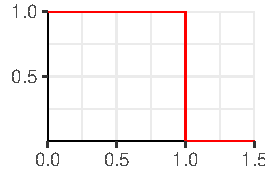
\includegraphics[scale=.4]{./img_ventanas/ventana_bartlett.pdf}\\
\rowcolor{gris}
Fejer &
$\displaystyle 
1-\abso{u}
$
& 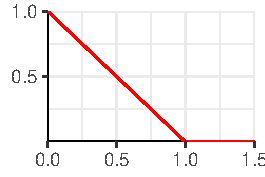
\includegraphics[scale=.4]{./img_ventanas/ventana_fejer.pdf} \\
Daniell &
$\displaystyle 
\frac{\SEN{\pi u}}{\pi u}
$
& 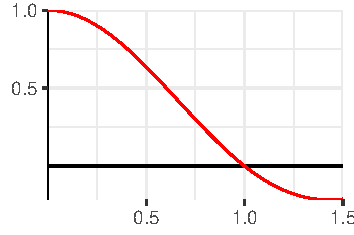
\includegraphics[scale=.4]{./img_ventanas/ventana_daniell.pdf} \\
\rowcolor{gris}
Bartlett-Priestley &
$\displaystyle 
\frac{3}{(\pi u)^{2}} \left[ \frac{\SEN{\pi u}}{\pi u} - \COS{\pi u} \right]
$
& 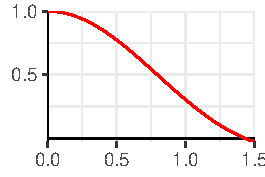
\includegraphics[scale=.4]{./img_ventanas/ventana_bartlet_priestley.pdf} \\
\bottomrulec
%\bottomrule
\end{tabular}
\end{small}
\end{table}

\begin{table}
\label{ventanas2}
\caption{Ejemplos de funciones ventana (función de transferencia)}
\centering
\begin{small}
\begin{tabular}{lll}
\toprule
Nombre & $K(\theta)$ & Bosquejo \\
\midrule
Bartlett &
$\displaystyle 
\frac{1}{\pi} \frac{\SEN{\theta}}{\theta}
$
& 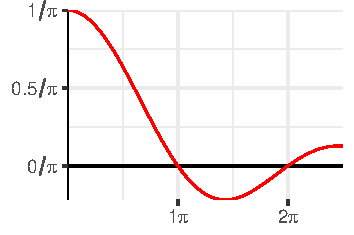
\includegraphics[scale=.4]{./img_ventanas/ventana_2_bartlett.pdf} \\
\rowcolor{gris}
Fejer &
$\displaystyle 
\frac{1}{2\pi} \left[ \frac{\SEN{\nicefrac{\theta}{2}}}{\nicefrac{\theta}{2}} \right]^{2}
$
& 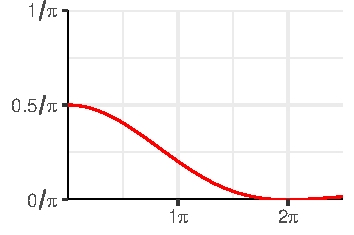
\includegraphics[scale=.4]{./img_ventanas/ventana_2_fejer.pdf} \\
Daniell &
$
\displaystyle 
\nicefrac{1}{2\pi} \text{, si } \abso{\theta}\leq \pi
$
& 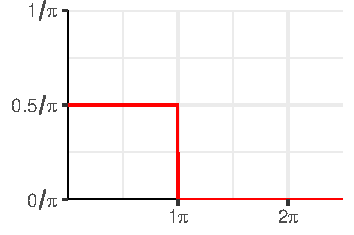
\includegraphics[scale=.4]{./img_ventanas/ventana_2_daniell.pdf} \\
\rowcolor{gris}
Bartlett-Priestley &
$\displaystyle 
\frac{3}{4 \pi} \left[ 1 - \left( \nicefrac{\theta}{\pi} \right) \right]
\text{, si } \abso{\theta}\leq \pi
$
& 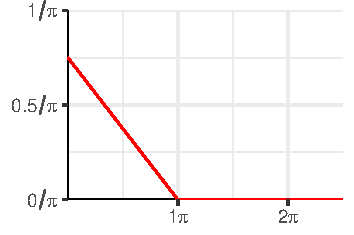
\includegraphics[scale=.4]{./img_ventanas/ventana_2_bartlet_priestley.pdf} \\
\bottomrulec
%\bottomrule
\end{tabular}
\end{small}
\end{table}

%%%%%%%%%%%%%%%%%%%%%%%%%%%%%%%%%%%%%%%%%%%%%%%%%%%%%%%%%%%%%%%%%%%%%%%%%%%%%%%%%%%%%%%%%%%%%%%%%%%
%%%%%%%%%%%%%%%%%%%%%%%%%%%%%%%%%%%%%%%%%%%%%%%%%%%%%%%%%%%%%%%%%%%%%%%%%%%%%%%%%%%%%%%%%%%%%%%%%%%

\section{Prueba de Priestley-Subba Rao}
\label{sec:psr}

La prueba de estacionariedad usada en el presente trabajo, fue propuesta por Priestley y Subba Rao en la década de 1960 \cite{Priestley69}.
%
Dicha prueba consiste en probar estadísticamente si el espectro evolutivo de un proceso dado puede reducirse a un espectro de potencias, como en el teorema \ref{lazy:redux}, lo cual es equivalente a probar si el proceso es débilmente estacionario.
%
El procedimiento consiste en los siguientes pasos:
\begin{enumerate}
\item Estimar el espectro evolutivo en algunos puntos en tiempo y frecuencia.
\item Calcular el logaritmo para \textit{estabilizar} al estimador.
\item Efectuar una ANOVA de dos vías para verificar si el espectro cambia en el tiempo.
\end{enumerate}

El primer paso, está sujeto a todas las restricciones descritas anteriormente en el presente capítulo.
%
Por notación, sea \xtd un proceso semi-estacionario a tiempo discreto, de media cero y varianza finita cuya frecuencia de muestreo es $\Delta_t=1$; y sea \xtd un conjunto de $N$ observaciones.
%
Usando esta información se calcula para estos datos el estimador de doble ventana, $\widehat{h}$; para ello se eligen las funciones ventana $g_\kappa$ y $w_\tau$ que, por simplicidad, son ventanas de escalamiento con parámetros $\kappa$ y $\tau$. 
%
Sus funciones de transferencia serán $\Gamma_\kappa$ y $W_\tau$, respectivamente.

%Considerando las propiedades de $\widehat{h}$ descritas en las proposiciones \ref{lazy:med_dd} y \ref{lazy:var_estdd}, y usando la aproximación del corolario \ref{detalle:aprox}, 
Se define al estimador $Y$ como
\begin{equation}
Y(t,\omega) = \log\left(\widehat{h}(t,\omega)\right)
\end{equation}

Como se dijo en la sección anterior, $Y$ satisface las siguientes propiedades
\begin{align}
\E{Y(t,\omega)} &\approx \log\left(h(t,\omega)\right) \\
\Var{Y(t,\omega)} &\approx \frac{C}{T} \intR \abso{\Gamma_\kappa(\theta)}^{4} d\theta
\end{align}

La \textit{forma} que tiene la varianza de $Y$ --aproximadamente constante-- sugiere que puede escribirse como
\begin{equation}
Y(t,\omega) = \log\left(\widehat{h}(t,\omega) \right) + \varepsilon(t,\omega)
\label{ye}
\end{equation}

Debido a la naturaleza discreta de los datos, conviene construir una malla de puntos en el tiempo y las frecuencias, equiespaciado en el tiempo por $\Delta_t$ y en las frecuencias por $\Delta_\omega$.
%
Si dichas distancias son suficientemente grandes como para que se cumplan las condiciones en \ref{separacion}, entonces los valores de $Y$ sobre la cuadrícula serán aproximadamente no-correlacionados.
%
\begin{equation}
\left.
\begin{aligned}
\intR \abso{\Gamma_\kappa(\theta)}^{2}\abso{\Gamma_\kappa(\theta+\Delta_\omega)}^{2} d\theta 
&\approx 0 \\
\frac{1}{\Delta_t} \intR \abso{t} \abso{w_\tau (t)} dt &\approx 0
\end{aligned}
\right\rbrace
\Rightarrow
\Cov{Y(t,\omega),Y(t+\Delta_t,\omega+\Delta_\omega)} \approx 0
\label{separacion}
\end{equation}
%
Así entonces, sea
$\left\{ (t_i,\omega_j) \in \mathcal{T} \times [-\pi,\pi] | i = 1,\dots,I ; j=1,\dots,J \right\}$
la cuadrícula descrita, con $\abso{t_i - t_{i+1}}= \Delta_t$ y 
$\abso{\omega_j-\omega_{j+1}}= \Delta_\omega$. 
%
Se construye una versión discretizada del estimador $Y$ como
\begin{equation}
Y_{i,j} := \log\left(\widehat{h}(t_i,\omega_j)\right)
\end{equation}
%
la cual satisface la versión discretizada de la expresión \ref{ye} 
\begin{equation}
Y_{i,j} \approx \log\left(h(t_i,\omega_j)\right) + \varepsilon_{i,j}
\label{def:ye}
\end{equation}
donde
\begin{align}
\E{\varepsilon_{i,j}} &\approx 0 \\
\Cov{\varepsilon_{i,j}} &\approx
\frac{C}{T} \intR \abso{\Gamma_\kappa(\theta)}^{4} d\theta \left[ \delta(i,i_0)\delta(j,j_0) \right]
\end{align}

Una vez descrito formalmente el efecto del logaritmo como estabilizador de $\widehat{h}$, conviene describir el efecto de la estacionariedad débil sobre $Y$.
%
Con base en la proposición \ref{lazy:redux}, si el proceso \xt es débilmente estacionario \textbf{entonces}
%
\begin{equation}
h(t_1,\omega_j) = h(t_2,\omega_j) = \cdots = h(t_I,\omega_j) \text{ , para } j = 1, 2, \dots , J
\label{h1}
\end{equation}
condición que puede reescribirse en términos de $Y$ como
%
\begin{equation}
\E{Y_{1,j}} = \E{Y_{2,j}} = \cdots = \E{Y_{I,j}} \text{ , para } j = 1, 2, \dots , J
\label{h2}
\end{equation}
%
la cual, a su vez, puede reescribirse como
\begin{equation}
\E{\varepsilon_{1,j}} = \E{\varepsilon_{2,j}} = \cdots = \E{\varepsilon_{I,j}} \text{ , para } j = 1, 2, \dots , J
\label{h3}
\end{equation}

Sin embargo, la expresión en \ref{h3} puede deducirse directamente de las propiedades de $Y$ en caso de que la expresión en \ref{h2} es cierta. 
%
En consecuencia, rechazar \ref{h3} implica rechazar \ref{h2}, lo cual aporta evidencia para rechazar \ref{h1}; si se rechaza \ref{h1} entonces puede rechazarse que el proceso sea estacionario, pero un no-rechazo no garantiza que el proceso sea estacionario.

El objetivo de la prueba puede fijarse en decidir si puede rechazarse la condición en \ref{h3}, en cuyo caso se podrá concluir que el proceso \textbf{no} es débilmente estacionario.
%
Con base a la expresión en \ref{h2}, la prueba puede formularse en términos de un ANOVA de dos vías (ver sección \ref{sec:ANOVA2}); para ello, se propone como hipótesis nula que $Y$ sigue el modelo general
%
\begin{equation}
H_0 : Y_{i,j} = \mu + \alpha_i + \beta_j + \gamma_{i,j} + \varepsilon_{i,j}
\end{equation}
%
donde $\varepsilon$ es como en la expresión \ref{def:ye}; se consideran a los parámetros $\alpha$, $\beta$, $\gamma$ normalizados de forma que
\begin{equation}
\sum_{i=1}^I \alpha_i = \sum_{j=1}^J \beta_j = \sum_{i=1}^I \sum_{j=1}^J \gamma_{i,j} = 0
\end{equation}

\begin{table}
\label{cantidades_psr}
\caption{Sumas de cuadrados en la prueba PSR}
\centering
\bordes{1.1}
\begin{tabular}{lll}
\toprule
Descripción & Estadístico & {Gr. de libertad} \\
\midrule
Efecto tiempo &
$S_T =J \sum_{i=1}^{I} \widehat{\alpha_i}^{2}$ 
& $I-1$ \\
Efecto frecuencia &
$S_F = I \sum_{j=1}^{J} \widehat{\beta_j}^{2}$ 
& $J-1$ \\
Interacción &
$S_{I+R} = \sum_{i=1}^{I} \sum_{j=1}^{J} 
\left( Y_{i,j} - \widehat{\alpha_i} - \widehat{\beta_j} - \widehat{\mu} \right)^{2}$ 
& $(I-1)(J-1)$ \\
%\midrule
\rowcolor{gris}
Total &
$S_{0} = \sum_{i=1}^{I} \sum_{j=1}^{J} 
\left( Y_{i,j} - \widehat{\mu} \right)^{2}$ 
& $IJ -1$ \\
\midrulec
Prom. general &
$\widehat{\mu} = \frac{1}{I J} \sum_{i=1}^{I} \sum_{j=1}^{J} Y_{i,j}$ & \\
Prom. tiempo &
$\widehat{\alpha_i} = \frac{1}{J} \sum_{j=1}^{J} Y_{i,j} - \widehat{\mu}$ & \\
Prom. frecuencia &
$\widehat{\beta_j} = \frac{1}{I} \sum_{i=1}^{I} Y_{i,j} - \widehat{\mu}$ & \\
\bottomrule
\end{tabular}
\end{table}

En la tabla \ref{cantidades_psr} se muestran las sumas de cuadrados asociadas al ANOVA.
%
Dentro del contexto de la estimación del espectro evolutivo, los parámetros involucradas pueden interpretarse como
\begin{description}
\item[$\mu$] Promedio de $Y$ sobre tiempo y frecuencia.
\item[$\alpha$] Efecto lineal sólo del tiempo.
\item[$\beta$] Efecto lineal sólo de la frecuencia.
\item[$\gamma$] Efecto lineal de tiempo y frecuencia.
\end{description}

Ahora bien, la expresión \ref{h2} puede formularse como hipótesis para contrastarse contra $H_0$, de la forma
%
\begin{equation}
H_A : \hspace{1em} Y_{i,j} = \mu + \alpha_i + \varepsilon_{i,j}
\end{equation}

Por simplicidad conviene considerar, como paso intermedio, una segunda prueba de hipótesis con una hipótesis \textit{intermedia} \textit{encadenada}
\begin{equation}
H_{A_0} : Y_{i,j} = \mu + \alpha_i + \beta_j + \varepsilon_{i,j}
\end{equation}

Para la prueba de hipótesis $H_0$ vs $H_{A_0}$ se usa el siguiente estadístico de prueba
\begin{equation}
\frac{\nicefrac{S_{I+R}}{(I-1)(J-1)}}{\nicefrac{S_0}{(IJ-1)}}
\sim F \left(\left(I-1 \right)\left(J-1 \right) , IJ-1 \right)
\end{equation}

En caso de que se rechace a $H_0$, se procede a realizar la prueba de hipótesis $H_{A_0}$ vs $H_{A}$, para lo cual se usa el siguiente estadístico de prueba
\begin{equation}
\frac{\nicefrac{S_{T}}{(I-1)}}{\nicefrac{S_0}{(IJ-1)}}
\sim F \left( I-1  , IJ-1 \right)
\end{equation}

Si se rechazan $H_0$ y $H_{A_0}$ (en ese orden), y se acepta $H_A$, entonces puede decirse que el registro corresponda a una observación de un proceso débilmente estacionario; por simplicidad, se dirá simplemente que la observación \textit{es} estacionaria.

Es importante enfatizar que, en el contexto de la estimación del espectro evolutivo, los resultados de la ANOVA adquieren una interpretación un tanto diferente a la usual: cuando el estadístico de prueba ocurre en la región de rechazo entonces se acepta que el \textit{efecto} del tiempo es estadísticamente significativo, y en consecuencia se acepta $H_0$ y se rechaza $H_{A_0}$. 
%
En el contraste de $H_{A_0}$ contra $H_A$ ocurre lo mismo.

Lo más común es rechazar la hipótesis nula --típicamente interpretada como un efecto negligible para un factor de interés-- si el estadístico de prueba supera un cierto valor umbral; en el caso de la prueba de PSR tal situación se invierte porque su hipótesis nula es un modelo general del cual se desean \textit{eliminar} ciertas variables cuyo efecto es negligible.
%
Todo este asunto se resuelve sencillamente reportando, el lugar del $p$-valor para el estadístico de prueba, el complemento a 1 de dicho valor.

Cabe mencionar que en gran parte del trabajo se usará la implementación de la prueba de PSR hecha por Constantine y Percival para el lenguaje de programación R \cite{R_fractal}.
%
En la siguiente subsección se muestra el uso de la prueba de PSR sobre dos ejemplos, y se compara la implementación en R.

%%%%%%%%%%%%%%%%%%%%%%%%%%%%%%%%%%%%%%%%%%%%%%%%%%%%%%%%%%%%%%%%%%%%%%%%%%%%%%%%%%%%%%%%%%%%%%%%%%%
%%%%%%%%%%%%%%%%%%%%%%%%%%%%%%%%%%%%%%%%%%%%%%%%%%%%%%%%%%%%%%%%%%%%%%%%%%%%%%%%%%%%%%%%%%%%%%%%%%%

\subsection{Ejemplos}
\label{sec:ejemplos}

El procedimiento de la prueba de PSR será usado primeramente en un proceso estocástico construido analíticamente para exhibir algunas características de interés (estacionariedad local); por fines ilustrativos se fingen desconocidas estas propiedades.
%
Posteriormente será usado un fragmento arbitrario de registro de PSG para una derivación arbitraria; esto con el fin de mostrar el método sobre un conjunto de datos con propiedades desconocidas.

Como primer ejemplo se construye al proceso $\{Z(t)\}_{t\in\R}$ como
\begin{equation}
Z(t) = \frac{1}{\sqrt{\psi(t)}} \int_{t-\nicefrac{\psi(t)}{2}}^{t+\nicefrac{\psi(t)}{2}} dW(u) 
\label{lazy20}
\end{equation}
donde $\{W(t)\}_{t\in\R}$ es un proceso de Wiener y la función $\psi:\R\rightarrow\R$ es como sigue
\begin{equation}
\psi(t) = \frac{1}{2} \left( \tanh(t) + 1 \right)
\end{equation}

El que el proceso $\{Z(t)\}_{t\in\R}$ sea construido de forma parecida a un proceso medias móviles sugiere que tiene propiedades similares, con algunas \textit{complicaciones} debido a que depende del tiempo.
%
En particular se usarán las mismas técnicas para calcular su valor esperado y núcleo de covarianza; con respecto al valor esperado:
\begin{align*}
\E{Z(t)} &= 
\E{\frac{1}{\sqrt{\psi(t)}} \int_{t-\nicefrac{\psi(t)}{2}}^{t+\nicefrac{\psi(t)}{2}} dW(u)} \\
&=
\frac{1}{\sqrt{\psi(t)}} \int_{t-\nicefrac{\psi(t)}{2}}^{t+\nicefrac{\psi(t)}{2}} \E{dW(u)} = 0
\end{align*}
posteriormente, respecto al núcleo de covarianza:
\begin{align*}
R(t,s) &= \E{Z(t)Z(s)} \\
&=
\E{\frac{1}{\sqrt{\psi(t)}\sqrt{\psi(s)}}
\int_{t-\nicefrac{\psi(t)}{2}}^{t+\nicefrac{\psi(t)}{2}} dW(u)
\int_{s-\nicefrac{\psi(s)}{2}}^{s+\nicefrac{\psi(s)}{2}} dW(v)
} \\
&= 
\frac{1}{\sqrt{\psi(t) \psi(s)}}
\E{\int_{\Omega_t \cap \Omega_s} du} \\
&= \max{ \left\{ \frac{\psi(t) + \psi(s) - 2 \abso{t-s}}{2\sqrt{\psi(t)\psi(s)}}, 0 \right\} }
\end{align*}
donde $\Omega_t = \left[ t-\nicefrac{\psi(t)}{2} , t+\nicefrac{\psi(t)}{2} \right]$, y similarmente para $\Omega_s$.
%
Con base a lo anterior, se puede deducir trivialmente que $\Var{Z(t)} = R(t,t) = 1$.

Se concluye que el proceso $\{Z(t)\}_{t\in\R}$ es de media 0 y varianza finita, pero no es débilmente estacionario porque no admite una función de autocorrelación.
%
Como su núcleo de covarianza es continuo en la diagonal $t=s$, el proceso es estocásticamente continuo.
%
Por simplicidad expositiva, se supondrá \textit{sin más} que $\{Z(t)\}_{t\in\R}$ es un proceso semi-estacionario.

En la figura \ref{fig:lazy21} se muestra una realización de $\{Z(t)\}_{t\in\R}$; el proceso fue discretizado usando $\Delta_Z=\nicefrac{1}{1000}$ en el intervalo $[-3.5,3.5]$, y posteriormente se reescaló el tiempo para usar $\Delta_Z=1$.
%
Conviene mencionar que este proceso fue construido para exhibir un comportamiento muy particular, que es \textit{visible} en su realización y en su núcleo de covarianza: 
\begin{itemize}
\item Si $0 \ll t$, entonces $\{Z(t)\}_{t\in\R}$ es aproximadamente un proceso medias móviles.
\item Si $0 \gg t$, entonces $\{Z(t)\}_{t\in\R}$ es aproximadamente un proceso ruido blanco.
\end{itemize}

\begin{figure}
\centering
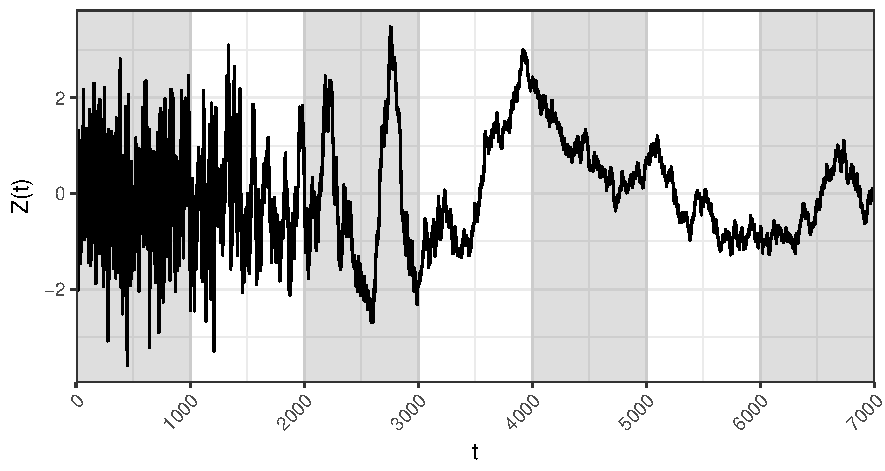
\includegraphics[width=0.9\linewidth]{./scripts_graf_res/proceso_Z.pdf}
\caption[Realización de un proceso estocástico, usado para ejemplificar la prueba de Priestley-Subba Rao]{Realización del proceso estocástico $\{Z(t)\}_{t\in\R}$, usado para ejemplificar el procedimiento de la prueba de PSR.}
\label{fig:lazy21}
\end{figure}

Una vez expuestas las características del proceso $\{Z(t)\}_{t\in\R}$, pero no su espectro evolutivo, se procede a aplicarle la prueba de PSR.

%%%%%%%%%%%%%%%%%%%%%%%%%%%%%%%%%%%%%%%%%%%%%%%%%%%%%%%%%%%%%%%%%%%%%%%%%%%%%%%%%%%%%%%%%%%%%%%%%%%
%%%%%%%%%%%%%%%%%%%%%%%%%%%%%%%%%%%%%%%%%%%%%%%%%%%%%%%%%%%%%%%%%%%%%%%%%%%%%%%%%%%%%%%%%%%%%%%%%%%

\subsubsection{Primer ejemplo}

Como primer paso se calcula el estimador de doble ventana, $\widehat{h}$, según la definición \ref{estimador_doble_ventana}; este estimador será calculado en una malla de puntos en el tiempo y las frecuencias.
%
para una malla de puntos en el tiempo y las frecuencias.
%
De manera concreta en este ejemplo, la malla es construida usando $\Delta_t = 1000$ y $\Delta_\omega=50$, con un total de 35 puntos.
%
Por simplicidad, conviene escribir nuevamente la expresión para $\widehat{h}$
\begin{equation}
\widehat{h}(\omega, t) = \sum_{u=T-t}^t w_\tau (u) \abso{U(\omega,t-u)}^{2}
\end{equation}
donde
\begin{equation}
U(t) = \sum_{u=T-t}^t g(u) X(t-u)
\end{equation}
%
En este ejemplo particular, se usa la ventana de Bartlett-Priestley, $k_\text{BP}$, para cubrir el papel de $g$ y $w_\tau$; esta función es tomada del cuadro \ref{ventanas} y escalada adecuadamente.
\begin{equation}
g_\tau(u) = w_\kappa(u) = \frac{1}{G_{\text{BP}}} k_{\text{BP}}\left( \nicefrac{u}{500} \right)
\end{equation}
donde
\begin{equation}
k_{\text{BP}} (u) = \begin{cases}
\frac{3}{\left( \pi u \right)^2} 
\left[ 
\frac{\SEN{\pi u}}{\pi u} - \COS{\pi u} \right] &, \abso{u} 
\leq 1 \\
0 &, \text{otro caso}
\end{cases}
\end{equation}
\begin{equation}
G_{\text{BP}} = \intR \left[ k_{\text{BP}}\left( \nicefrac{u}{500} \right) \right]^2 du
\end{equation}

Bajo estas instrucciones es claro cómo calcular los valores de $\widehat{h}$ y $Y = \log\left( \widehat{h} \right)$; estos valores se muestran en el cuadro \ref{tab:valores_psr}.
%
Con fines de claridad, en la figura \ref{fig:proceso_psr} se enfatiza esquemáticamente la interpretación que tienen dichas cantidades.

\begin{table}
\label{tab:valores_psr}
\caption{Promedios del estimador $Y$ para el primer ejemplo}
\centering
\begin{tabular}{lrrrrrrr}
\toprule
      & \multicolumn{6}{l}{Frecuencia $\omega_i$} \\
\cmidrule{2-7}
      & $j=1$  & $j=2$   & $j=3$   & $j=4$   & $j=5$   & $j=6$   & $\widehat{\alpha_i}$ \\ 
\midrule
$i=1$ & -4.504 & -5.328  & -8.623  & -6.393  & -8.953  & -9.340  & 2.155  \\
$i=2$ & -1.418 & -7.526  & -8.463  & -11.453 & -9.392  & -9.381  & 1.406  \\
$i=3$ & -1.315 & -9.812  & -10.681 & -11.370 & -12.126 & -11.837 & -0.179 \\
$i=4$ & 1.462  & -9.852  & -10.176 & -10.732 & -11.823 & -11.880 & 0.511  \\
$i=5$ & -1.159 & -11.056 & -12.269 & -14.145 & -12.297 & -12.965 & -1.304 \\
$i=6$ & 0.221  & -10.473 & -11.111 & -12.568 & -13.392 & -14.044 & -0.883 \\
$i=7$ & -2.713 & -11.255 & -12.739 & -13.670 & -13.560 & -12.373 & -1.707 \\
$\widehat{\beta_j}$
      & 7.998  & 0.016   & -1.235  & -2.131  & -2.304  & -2.344  &         \\ 
\bottomrule
\end{tabular}
\end{table}

A partir de los datos del cuadro \ref{tab:valores_psr} efectúa el ANOVA de dos vías usando los estimadores descritos en el cuadro \ref{cantidades_psr}.
%
Primeramente se calcula el promedio global $\widehat{\mu} = -9.345$; posteriormente se calculan $\widehat{\alpha_i}$ y $\beta_j$ para $i=1,\dots, 7$ y $j=1,\dots, 6$, respectivamente. 
%
Después se calculan las sumas de cuadrados, estas últimas reportadas en el cuadro \ref{tab:ejemplo_gl}.
%
Finalmente se calculan los estadísticos de prueba
\begin{align}
F_{I+R} &= \frac{\nicefrac{S_{I+R}}{(I-1)(J-1)}}{\nicefrac{S_0}{(IJ-1)}} = 0.589 \\
F_{T} &= \frac{\nicefrac{S_{T}}{(I-1)}}{\nicefrac{S_0}{(IJ-1)}} = 0.112
\end{align}

Se calcula el p-valor de los estadísticos de prueba comparándolos con las distribuciones de los estadísticos: $F$ de Fisher con $(6,34)$ y $(30,34)$ grados de libertad, respectivamente.
%
Como se mencionó, la decisión de la prueba de PSR en base a los p-valores es \textit{opuesta} a los ANOVA usuales: como hay suficiente información para afirmar que $F_{I+R} \neq 0$, entonces se acepta que el proceso es no-estacionario.
%
Cabe recalcar que la decisión sobre estacionariedad se hace aún sin consultar a $F_T$.

\begin{table}
\label{tab:ejemplo_gl}
\centering
\caption{ANOVA de la prueba PSR para el primer ejemplo}
\begin{tabular}{llrrrrrr}
\toprule
\multicolumn{2}{l}{Efecto}
                        & GL & Total   & Promedio & $F$   & $p$     & $1-p$   \\
\midrule
$S_T$     & Tiempo      & 6  & 73.834  & 12.306   & 0.589 & 0.26290 & 0.73710 \\
$S_F$     & Frecuencia  & 5  & 565.891 & 113.178  & 5.420 & 0.99935 & 0.00065 \\
$S_{I+R}$ & Interacción & 30 & 70.247  & 2.342    & 0.112 & 0.00000 & 1.00000 \\
$S_0$     & Total       & 34 & 709.972 & 20.882   &       &         &         \\
\bottomrule
\multicolumn{5}{l}{GL = Grados de libertad}
\end{tabular}
\end{table}

\begin{figure}
\centering
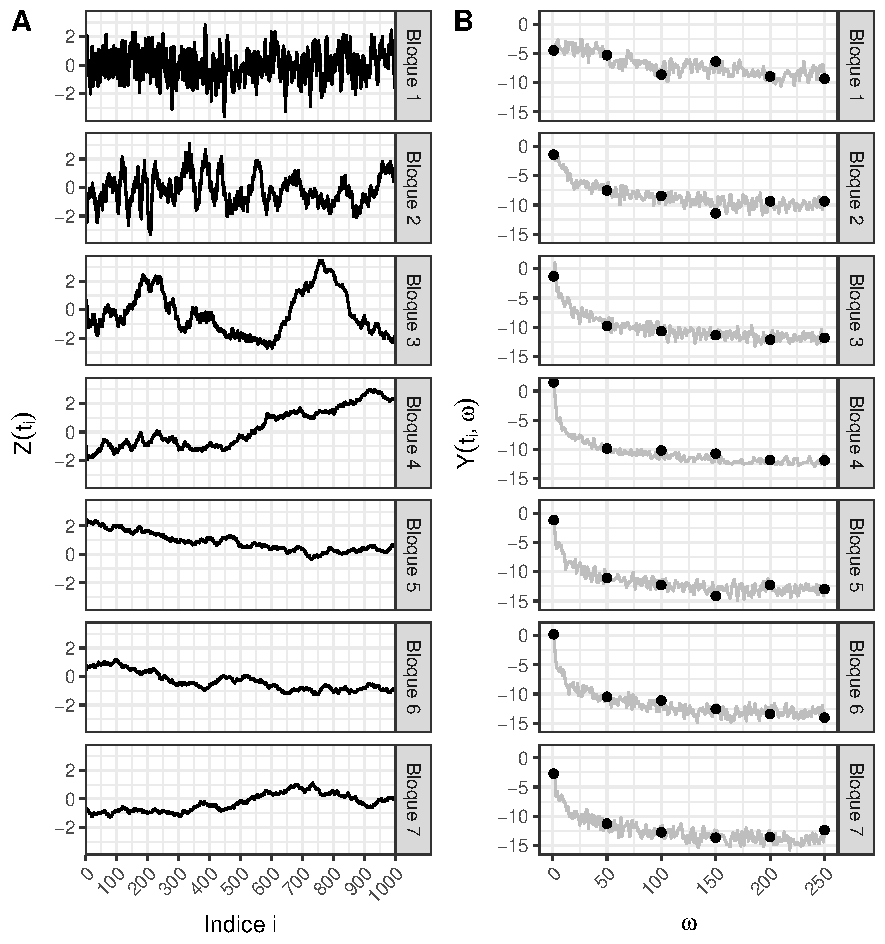
\includegraphics[width=\linewidth]{./scripts_graf_res/proceso_Z_fragmentado_doble.pdf}
\caption[Algunos pasos en el cálculo del estimador $Y$]{Ilustración de algunos pasos en el cálculo del estimador $Y$ sobre la malla de puntos $\{ t_1, t_2, \dots, t_I\} \times \{\omega_1, \omega_2, \dots, \omega_J\}$.
\textbf{A.}
Realización del proceso estocástico $\{Z(t)\}_{t\in\R}$, fragmentada en bloques de longitud $\Delta_t$. 
%
Los puntos en el $i$--ésimo bloque son usados para calcular $Y_{i,j}$ en los puntos $\omega_1, \omega_2, \dots, \omega_J$.
\textbf{B.}
Estimador $Y$, calculado para los bloques definidos anteriormente.
%
Por fines expositivos se grafica a $Y(t_i,\bullet)$ para diferentes valores de $\omega$, y posteriormente se marcan con puntos los valores correspondientes a la malla.}
\label{fig:proceso_psr}
\end{figure}

Para el análisis anterior se usó una cantidad muy baja de puntos con el fin de ilustrar claramente cómo son procesados estos datos.
%
Una versión más realista requiere usar la mayor cantidad de puntos posibles en el tiempo y las frecuencias, pero que sean tales que se cumplan las aproximaciones usadas; en principio no existen criterios para hallar estos parámetros de forma óptima, al menos no si las propiedades de los datos son desconocidas.

En la implementación del comando \texttt{stationarity} se sugiere que el número de bloques sea $\entero{\log_2(N)}$, con $N$ el número total de puntos considerados y $\entero{\bullet}$ la función parte entera, y $\Delta_\omega=6$.

%%%%%%%%%%%%%%%%%%%%%%%%%%%%%%%%%%%%%%%%%%%%%%%%%%%%%%%%%%%%%%%%%%%%%%%%%%%%%%%%%%%%%%%%%%%%%%%%%%%%%%%%%%%%%%%%%%%%%%%%%%%%%%%%%%%%%%%%%%%%%%%%%%%%%%%%%%%%%%%%%%%%%%%%%%%%%%%%%%%%%%%%%%%%%%%%%%%%%%

\subsubsection*{Segundo ejemplo}

Como segundo ejemplo se usa un fragmento arbitrario de registro de PSG; en particular se ha usado una época\footnote{La palabra `época' es usada como sinónimo de `fragmento de registro' por concordancia con la literatura sobre registros electrofisiológicos.} de 30 segundos de duración, correspondiente a la derivación Fp2 registrada en el participante MHJ durante sueño MOR; en la sección \ref{sec:eeg} se explica a detalle el significado de estos términos.
%
El registro fue efectuado usando una frecuencia de muestreo de 512 Hz ($\Delta_X =\nicefrac{1}{512}$), de modo que se contemplan 15,360 puntos; éstos mismos puntos son graficados en la figura \ref{fig:lazy22}.

Cabe destacar que este fragmento de registro no fue elegido para representar alguna característica en particular sino, más bien, el comportamiento general de los registros de PSG durante sueño MOR.

\begin{figure}
\centering
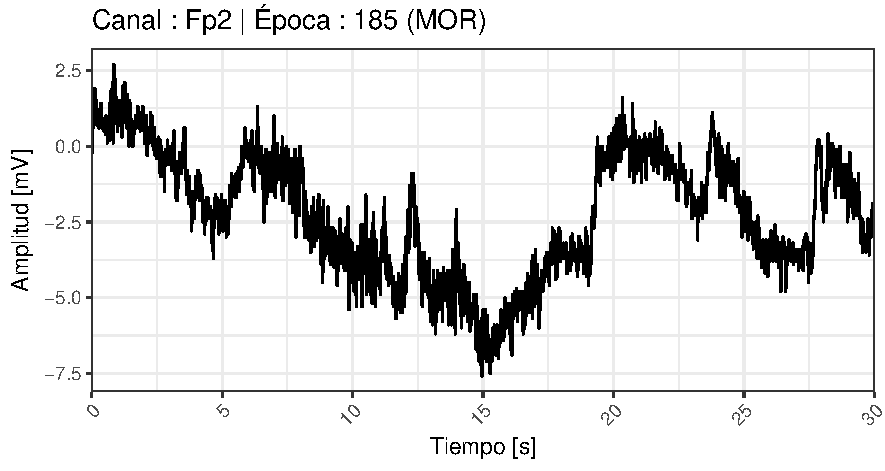
\includegraphics[width=.9\linewidth]{./scripts_graf_res/psg.pdf}
\caption[Fragmento de registro de PSG, usado para ejemplificar la prueba de Priestey-Subba Rao]{Fragmento de registro de PSG, usado para ejemplificar el procedimiento de la prueba de PSR.
%
El fragmento, referido como época, corresponde a 30 segundos registradas con una frecuencia de muestreo de 512 Hz; posteriormente fue reindexado.}
\label{fig:lazy22}
\end{figure}

El estimador $Y$ es calculado de la misma forma que en el ejemplo anterior; en esta ocasión simplemente se reportan los resultados en las tablas \ref{tab:valores_psr_2} y \ref{tab:ejemplo_gl_2}.
%
Para estos datos se calcula que $\widehat{\mu} = -9.265$; aunque este dato no se reporta en las tablas, efectivamente es importante. 

Tras revisar los estadísticos de prueba se decide, como se esperaba intuitivamente, que el fragmento de registro es no-estacionario.

\begin{table}
\label{tab:valores_psr_2}
\caption{Promedios del estimador $Y$ para el segundo ejemplo}
\centering
\begin{tabular}{lrrrrrrr}
\toprule
      & \multicolumn{6}{l}{Frecuencia $\omega_i$} \\
\cmidrule{2-7}
      & $j=1$  & $j=2$   & $j=3$   & $j=4$   & $j=5$   & $j=6$   & $\widehat{\alpha_i}$ \\ 
\midrule
$i=1$ & -0.858 & -9.903  & -11.987 & -12.942 & -11.632 & -11.962 & -0.616 \\
$i=2$ & 1.709  & -10.475 & -11.567 & -12.401 & -12.267 & -13.068 & -0.413 \\
$i=3$ & 3.701  & -8.860  & -9.321  & -10.844 & -11.392 & -12.501 & 1.062  \\
$i=4$ & 3.236  & -9.175  & -10.387 & -12.345 & -14.106 & -12.106 & 0.118  \\
$i=5$ & 1.474  & -10.461 & -11.116 & -12.332 & -12.835 & -13.399 & -0.513 \\
$i=6$ & 1.442  & -9.301  & -10.257 & -10.947 & -12.500 & -11.852 & 0.362  \\
$\widehat{\beta_j}$
     & 11.049 & -0.431  & -1.508  & -2.704  & -3.190  & -3.216  &         \\
\bottomrule
\end{tabular}
\end{table}

\begin{table}
\label{tab:ejemplo_gl_2}
\centering
\caption{ANOVA de la prueba PSR para el segundo ejemplo}
\begin{tabular}{llrrrrrr}
\toprule
\multicolumn{2}{l}{Efecto}
                        & GL & Total   & Promedio & $F$   & $p$     & $1-p$   \\
\midrule
$S_T$     & Tiempo      & 5  & 12.520  & 2.504   & 0.093 & 0.00721 & 0.99279 \\
$S_F$     & Frecuencia  & 5  & 914.235 & 182.847 & 6.774 & 0.99984 & 0.00016 \\
$S_{I+R}$ & Interacción & 25 & 17.998  & 0.720   & 0.027 & 0.00000 & 1.00000 \\
$S_0$     & Total       & 35 & 944.753 & 26.993  &       &         &         \\
\bottomrule
\multicolumn{5}{l}{GL = Grados de libertad}
\end{tabular}
\end{table}

%\subsubsection*{Comentarios sobre la implementación}

%%%%%%%%%%%%%%%%%%%%%%%%%%%%%%%%%%%%%%%%%%%%%%%%%%%%%%%%%%%%%%%%%%%%%%%%%%%%%%%%%%%%%%%%%%%%%%%%%%%
%%%%%%%%%%%%%%%%%%%%%%%%%%%%%%%%%%%%%%%%%%%%%%%%%%%%%%%%%%%%%%%%%%%%%%%%%%%%%%%%%%%%%%%%%%%%%%%%%%%

\section{Estacionariedad local}
\label{sec:est_local}

Conviene destacar que el objetivo central del presente trabajo es utilizar las herramientas descritas anteriormente (en especial la prueba de PSR) sobre registros de PSG en adultos mayores.
%
Para que los análisis sean significativos, desde el punto de vista fisiológico, deben resaltarse algunos \textit{comportamientos} esperados; en otras palabras, algunas propiedades de estas señales  se deben considerar conocidas a priori, con base a lo que se ha reportado en la literatura.
%
De forma particular, se ha propuesto que el cerebro es un mecanismo con una gran \textit{complejidad} asociada \cite{Werner09}.

Bajo este contexto se entiende a la complejidad como la presencia de características propias de un conjunto de elementos, que inducen {estados} independientes de los elementos individuales, pero que dependen \textit{críticamente} de parámetros macroscópicos.
%
Un ejemplo sencillo es la solidificación del agua, que depende principalmente de la temperatura y permite múltiples estados de equilibrio macroscópicos (la forma del hielo) que no están determinados por las partículas de agua; cerca de la temperatura de congelamiento el agua pasa de líquido a sólido, sin permitir estados intermedios.

La complejidad del cerebro se deduce de la existencia de múltiples niveles de organización, que corresponden a comportamientos cualitativamente diferentes --los cuales deben ser modelado usando herramientas que respeten tales diferencias.
%
Como ejemplo pueden mencionarse los campos eléctricos inducidos por neuronas individuales y por grandes conjuntos de neuronas; estos dos fenómenos están estrechamente relacionados de manera intuitiva, pero cualitativamente son abismalmente diferentes.
%
En el libro \textit{``Mathematical Foundations of Neuroscience"}, por G. Bard Ermentrout \cite{Ermentrout10}, se describe a detalle cómo los potenciales para neuronas pueden modelarse satisfactoriamente mediante el sistema de ecuaciones diferenciales de Hodgkin--Huxley; en contraparte, los \textit{potenciales de campo} responden mejor al sistema de ecuaciones diferenciales estocásticas Wilson--Cowan.

Para el caso muy concreto del EEG, se ha propuesto la complejidad de la actividad eléctrica cerebral se traduce en la {orquestación} de múltiples estados de actividad a lo largo del tiempo \cite{kaplan2000application}. 
%
En otras palabras, el EEG es una señal compleja que está formada por una gran variedad de fragmentos \textit{simples}; en concreto, se espera que estos fragmentos sean débilmente estacionarios.
%
Concordando con la definición formal hecha sobre el tema por Rainer Dahlhaus \cite{Dahlhaus97}, este fenómeno será referido como \underline{estacionariedad local}.

Bajo el supuesto de la estacionariedad local el EEG es un fenómeno globalmente heterogéneo pero localmente homogéneo; en consecuencia el EEG es globalmente no-estacionario, pero es posible segmentarlo en fragmentos que son débilmente estacionarios.
%
Dentro de esta línea de pensamiento se espera que los fragmentos de EEG débilmente estacionarios --o que clasifiquen como estacionarios según la prueba de PSR, en concreto-- se \textit{agrupen} replicando algún nivel de organización.

\begin{figure}
\centering
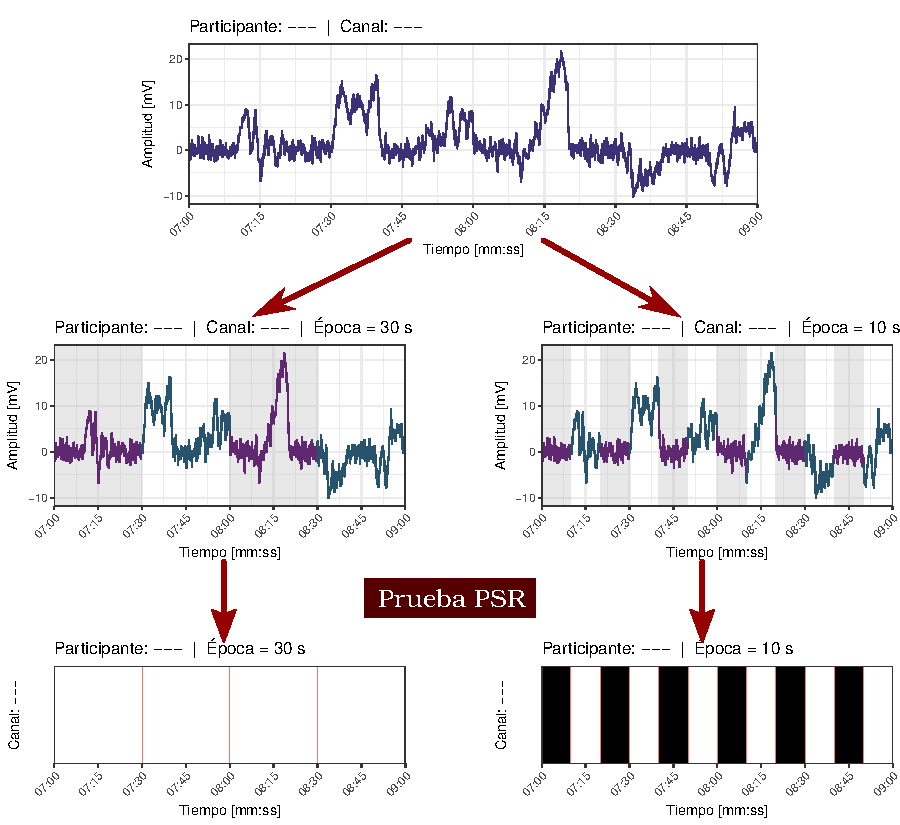
\includegraphics[width=\linewidth]{./img_diagramas/epocas_diferentes_v3.pdf}
\caption[Efecto esperado del tamaño de ventana sobre la clasificación de estacionariedad, bajo el supuesto de estacionariedad local]{Efecto esperado del tamaño de ventana sobre la clasificación de estacionariedad, bajo el supuesto de estacionariedad local.
%
Suponiendo que la señal es heterogénea, pero que está \textit{compuesta} por múltimples fragmentos homogéneo de duración corta, entonces al disminuir el tamaño de ventana se espera \textit{hallar} con mayor frecuencia estos fragmentos homogéneos.
%
Adaptado de \cite{FRONTIERS}.
}
\label{epocas_diferentes}
\end{figure}

De manera pragmática y de acuerdo a los protocolos (ver más adelante), los registros de PSG son segmentados en ventanas sin traslape con una duración fija decidida a priori.
%
Así entonces, se espera que el efecto de la estacionariedad local se más notorio al cambiar el tamaño de tales segmentos; este procedimiento se ilustra en la figura \ref{epocas_diferentes}, así como el efecto esperado sobre la clasificación de estacionariedad.


Cabe destacar que bajo este supuesto, surge la pregunta sobre hasta qué punto es posible es posible modelar efectivamente al EEG como señales aleatorias con propiedades \textit{simples}.
%
En varios trabajos pioneros \cite{Cohen77,Kawabata73,McEwen75,Sugimoto78} se demuestra experimentalmente que el EEG puede considerarse estacionario si se usan segmentos de hasta 20 segundos, e incluso se sugiere que esta cantidad puede cambiar para personas con daños neuronales.
%
Esta pregunta es explorada en el presente trabajo repitiendo la prueba de PSR para diferentes tamaños de ventana.
%
Es importante considerar, debido a la --posible-- variabilidad en el tiempo, el efecto de tomar una cantidad menor de puntos es cualitativamente diferente al efecto de, por ejemplo, considerar una frecuencia de muestreo menor.

Por ejemplo, considérese al primer ejemplo de la sección anterior, el proceso $\{Z(t)\}$, que es aproximadamente un proceso ruido blanco para $t\ll 0$ y aproximadamente un proceso medias móviles para $t \gg 0$; este proceso es localmente estacionario por diseño.
%
En la figura \ref{lazy_fin} se efectúa esta clasificación repetida para diversos tamaños de ventana, revelando que los fragmentos pequeños son clasificados como estacionarios.
%
Este efecto era de esperarse por la descripción de estacionariedad local: un fenómeno que es globalmente heterogéneo pero que está \textit{compuesto} por fragmentos homogéneos.

\begin{figure}
\centering
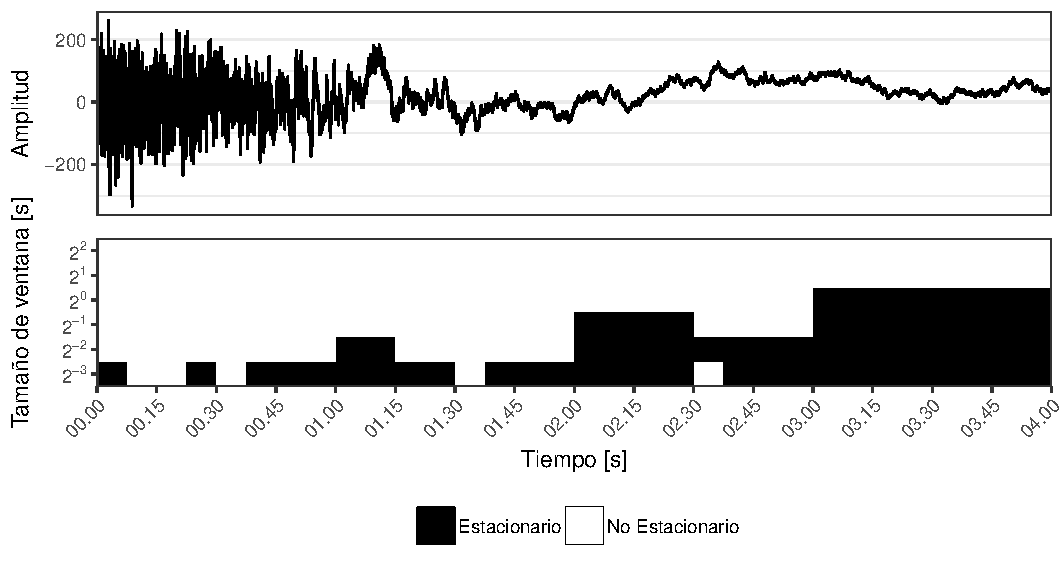
\includegraphics[width=\linewidth]{./scripts_graf_res/stat_local_artificial.pdf}
\caption[Ejemplo de cambios en la clasificación de estacionariedad débil al cambiar el tamaño de ventana]{Ejemplo de cambios en la clasificación de estacionariedad débil, según la prueba de PSR, usando diferentes tamaños de ventana y un proceso localmente estacionario.
%
En la parte superior se muestra a la señal usada ejemplo, una realización para un proceso estocástico localmente estacionario cuyas propiedades se describen en el texto.
%
En la parte inferior se muestran las ventanas usadas para segmentar la señal, las cuales fueron coloreadas según si dicho fragmento de señal fue clasificado como estacionario.
%
Puede notarse cómo la señal es efectivamente estacionaria, pero algunos fragmentos pequeños son clasificados como estacionarios.
}
\label{lazy_fin}
\end{figure}

Posteriormente se replica este análisis para los registros de PSG en el total de su duración.
%
Los tamaños de ventana se tomaron de la forma $30 \times 2^{n}$ segundos, por compatibilidad con las ventanas de 30 segundos (recomendación protocolaria de la AASM); para más detalles sobre el procedimiento, ver la sección \ref{sec:analisis_registro}. 
%
Conviene mencionar que esta metodología es similar a aquella usada por McEwen en 1975 \cite{McEwen75}.

%%%%%%%%%%%%%%%%%%%%%%%%%%%%%%%%%%%%%%%%%%%%%%%%%%%%%%%%%%%%%%%%%%%%%%%%%%%%%%%%%%%%%%%%%%%%%%%%%%%
%%%%%%%%%%%%%%%%%%%%%%%%%%%%%%%%%%%%%%%%%%%%%%%%%%%%%%%%%%%%%%%%%%%%%%%%%%%%%%%%%%%%%%%%%%%%%%%%%%%
%%%%%%%%%%%%%%%%%%%%%%%%%%%%%%%%%%%%%%%%%%%%%%%%%%%%%%%%%%%%%%%%%%%%%%%%%%%%%%%%%%%%%%%%%%%%%%%%%%%
%%%%%%%%%%%%%%%%%%%%%%%%%%%%%%%%%%%%%%%%%%%%%%%%%%%%%%%%%%%%%%%%%%%%%%%%%%%%%%%%%%%%%%%%%%%%%%%%%%%

\chapter{Deterioro cognitivo y sueño}

En este capítulo se exponen varios temas para poder entender adecuadamente al sujeto de estudio (registros de PSG en adultos mayores), así como el contexto y la motivación para su estudio (el Posible Deterioro Cognitivo Leve, PDCL, en adultos mayores).
%
Se responden, de manera muy breve, las siguientes preguntas:
\begin{itemize}
\item ¿Qué es el Deterioro Cognitivo Leve y cómo se diagnostica?
\item Clínicamente, ¿qué es el sueño y cómo se estudia?
\item ¿Cómo se relacionan el Deterioro Cognitivo Leve y el sueño?
\end{itemize}

Para simplificar la exposición, se considera a la Electroencefalografía como a la técnica principal para el estudio de la actividad cerebral;
%
con la misma intención, se describe primero al sueño (desde el punto de vista clínico) y posteriormente su posible utilidad como marcador para el DCL.

El lector interesado en una exposición amplia sobre técnicas para el estudio del cerebro, puede referirse al libro \textit{``Medical Instrumentation. Applications and Design"} por John Webster \cite{Webster}; en contraparte, para obtener más información sobre el EEG es recomendable el libro \textit{``Electroencephalography: Basic Principles, Clinical Applications, and Related Fields"} por Ernst Niedermeyer \cite{niedermeyer}.
%
Para indagar más sobre las pruebas neuropsicológicas y su uso diagnóstico, se recomienda el libro \textit{``Guía para el diagnóstico neuropsicológico"} por Ardila y Ostrosky \cite{Ardila12}.
%
Si se desean revisar a detalle los protocolos para registrar la PSG, o aquellos para clasificar las etapas de sueño, debe consultarse el Manual de la AASM \cite{AASM07}.
%
Para aprender más sobre el sueño, así como los procesos fisiológicos y psicológicos asociados, puede consultarse el libro \textit{``Psicofisiología del sueño"} de Corsi-Cabrera \cite{Corsi1983}.

%%%%%%%%%%%%%%%%%%%%%%%%%%%%%%%%%%%%%%%%%%%%%%%%%%%%%%%%%%%%%%%%%%%%%%%%%%%%%%%%%%%%%%%%%%%%%%%%%%%
%%%%%%%%%%%%%%%%%%%%%%%%%%%%%%%%%%%%%%%%%%%%%%%%%%%%%%%%%%%%%%%%%%%%%%%%%%%%%%%%%%%%%%%%%%%%%%%%%%%

\section{Deterioro Cognitivo Leve}
\label{seccion:dcl}

El envejecimiento es determinado por una serie de procesos moleculares, celulares, fisiológicos y psicológicos que conducen directamente al deterioro de funciones cognitivas, específicamente atención y memoria \cite{Park09}.
%
Como consecuencia, los \textbf{adultos mayores} son especialmente propensos al deterioro cognitivo; por precisión, en lo siguiente se usará el término \textit{adulto mayor} para referirse a individuos con 60 o más de edad años.
%
Cabe destacar que la funcionalidad del adulto mayor no depende meramente de la edad, sino que está relacionada con el estilo de vida, los factores de riesgo, el acceso a la educación y las acciones para el cuidado de la salud realizadas en edades más tempranas \cite{Sanhueza14}.
 
La \textbf{demencia}, considerada como el estado más grave del deterioro cognitivo, es definida en el Manual Diagnóstico y Estadístico de Trastornos Mentales (DSM-V, por sus siglas en inglés y la versión consultada) como sigue:
\begin{quote}
``Un síndrome que consiste en el desarrollo de déficits cognoscitivos suficientemente graves como para interferir significativamente en las actividades laborales y sociales, respecto al nivel de actividad previo.\\
%
Los sujetos con demencia tienen una baja capacidad para aprender información nueva y suelen olvidar lo aprendido anteriormente, siendo éste el síntoma más prominente."  \cite{DCM5}
\end{quote}

Hasta el momento se considera que la demencia es irreversible, y no se han identificado curas \cite{PlanAlzheimer04}. 
%
Debido a ello, ha surgido un gran interés en definir y diagnosticar sus etapas tempranas. 
%
El diagnóstico temprano es importante para un tratamiento adecuado que revierta o desacelere el avance de este síndrome \cite{Knopman01}.

Bajo esta línea de pensamiento se considera al \textbf{Deterioro Cognitivo Leve} (DCL) como una etapa precursora de la demencia, y que es definida como sigue: 
\begin{quote}
``Una alteración adquirida y prolongada de una o varias funciones cognitivas, que no corresponde a un síndrome focal y no cumple criterios suficientes de gravedad para ser calificada como demencia." \cite{Robles02}
\end{quote}

Para fines de la definición anterior, se entiende por \textit{síndrome focal} al daño en una estructura nerviosa específica, cuya causa es conocida (como una hemorragia o una embolia) y cuyo inicio sea inmediato y evidente. 

El DCL puede detectarse por medio de diversos métodos, que pueden ser complementarios entre sí. 
%
La forma de detección más simple es la percepción de fallas en la memoria por parte del individuo o de otro. 
%
La percepción subjetiva del deterioro cognitivo \textit{esperado} por el envejecimiento provoca que esta forma de detección sea poco fiable.
%
Una alternativa más {formal} consiste en la entrevista clínica de un especialista, la aplicación de cuestionarios sobre dificultades en la memoria, o incluso el uso de pruebas neuropsicológicas. 

En psicología, los instrumentos de medición comunes son las \textbf{pruebas neuropsicológicas}, 
entendidas como muestras de alguna conducta de interés a las que se asignan puntajes para comparar 
cuantitativamente a los sujetos \cite{Ardila12}.
%
Se considera que a través de estas herramientas es posible declarar objetivamente las deficiencias cognitivas o conductuales de los individuos, así como su severidad y características.

De forma auxiliar para el diagnóstico del DCL, se pueden efectuar análisis genéticos, químicos, de imágenes cerebral, entre otros que estudien el sistema nervioso central.
%
Se espera que dichas técnicas, en combinación con las pruebas neuropsicológicas, permitan diagnosticar más acertadamente el DCL y desentrañar los fenómenos neurobiológicos subyacentes.

Un referente ampliamente usado para el diagnóstico del DCL son los criterios para Alzheimer de la NINCDS--ADRDA, propuestos %en 1984 
por el \textit{National Institute of Neurological and Communicative Disorders and Stroke} y la \textit{Alzheimer's Disease and Related Disorders Association} 
%\cite{McKhann,Dubois07}. 
\cite{Dubois07}. 
%
Dichos criterios proporcionan protocolos para diagnosticar el Alzheimer y algunas enfermedades relacionadas (entre ellas el DCL), así como afecciones que generan síntomas similares. 
%
Desafortunadamente, las pruebas neuropsicológicas contempladas por los criterios de la NINCDS--ADRDA todavía no han sido \textit{validadas} en México, es decir que su efectividad para generar diagnósticos acertados no ha sido verificada para la población mexicana. 

Otra prueba neuropsicológica ampliamente extendida es el Mini-Mental State Examination (MMSE), propuesta por Folstein en 1975 \cite{folstein75}. %[citar mas, quiza??].
%
Sin embargo se ha reportado que, en la población mexicana, la prueba MMSE tiene baja sensibilidad para el diagnóstico de DCL en general, y baja especificidad para individuos con escolaridad muy baja o muy alta \cite{Ostrosky00}.
%
Para fines del comentario anterior, se entiende por \textit{sensibilidad} a la probabilidad de obtener verdaderos positivos, y por \textit{especificidad} a la probabilidad de obtener verdaderos negativos.

Una tercera opción, a la cual se ha dado gran peso en el presente trabajo, es la prueba neuropsicológica Neuropsi, desarrollada por Ostrosky y colaboradores en la Universidad Autónoma de México (UNAM) \cite{Ostrosky1999}.
%
La prueba Neuropsi ha sido validada para diversos grupos poblacionales en México, y se ha confirmado su utilidad para distinguir individuos con diverso grado de deterioro cognitivo.

En el contexto de la detección del DCL, es muy importante realizar un diagnóstico diferencial con respecto a la \textbf{pseudodemencia depresiva}, una afección que puede confundirse con el deterioro cognitivo.
%
De acuerdo al manual DSM-V, pseudodemencia depresiva se define como \textit{``un trastorno del afecto y que produce un aparente deterioro cognitivo"} \cite{DCM5}.
%
Bajo esta línea de pensamiento resulta conveniente decir que, como parte del diseño experimental, se han omitido participantes con síndromes focales, retraso mental, bipolaridad, esquizofrenia, entre otros trastornos de atención y memoria ajenos al deterioro cognitivo. 
%
Con base a lo anterior, se omite una discusión más extensa de dicho tipo de afecciones; el lector interesado puede referirse al Manual DSM-V \cite{DCM5}.

%%%%%%%%%%%%%%%%%%%%%%%%%%%%%%%%%%%%%%%%%%%%%%%%%%%%%%%%%%%%%%%%%%%%%%%%%%%%%%%%%%%%%%%%%%%%%%%%%%%
%%%%%%%%%%%%%%%%%%%%%%%%%%%%%%%%%%%%%%%%%%%%%%%%%%%%%%%%%%%%%%%%%%%%%%%%%%%%%%%%%%%%%%%%%%%%%%%%%%%

\subsection{Probable Deterioro Cognitivo Leve}

En el presente trabajo se delimita al DCL por fines de precisión, usando para ello las pruebas neuropsicológicas. 
%
Se define operativamente al \textbf{Posible Deterioro Cognitivo Leve} (PDCL) como sigue:
\begin{quote}
``Una disminución significativa de las funciones cognitivas del sujeto con respecto las típicas de su edad y nivel de educación."
\end{quote}

Para fines de la definición anterior, el desempeño de las funciones cognoscitivas en un individuo es medido usando la prueba Neuropsi \cite{Ostrosky1999}; se considera que hay un déficit cognoscitivo \textit{significativo} si la puntuación obtenida es menor al umbral predefinido para su grupo de edad y nivel de escolaridad.
%
El umbral recomendado para la prueba Neuropsi debe calcularse como la media menos 3 desviaciones estándar de los puntajes típicos para individuos de cada grupo de edad y nivel de escolaridad; estos parámetros fueron estimados para la población mexicana por Ostrosky-Solís y colaboradores \cite{Ostrosky1999}.
%
En el cuadro \ref{anexo:neuropsi}, bajo la etiqueta \textit{Deterioro cognitivo} se recaban los \textit{puntajes de corte} usados para declarar el PDCL.

La palabra \textit{`probable'} en el PDCL hace alusión a que no constituye un diagnóstico \textit{irrefutable} del DCL.
%
En este sentido, el PDCL puede interpretarse como una condición \textit{necesaria pero no suficiente} para el DCL.

%%%%%%%%%%%%%%%%%%%%%%%%%%%%%%%%%%%%%%%%%%%%%%%%%%%%%%%%%%%%%%%%%%%%%%%%%%%%%%%%%%%%%%%%%%%%%%%%%%%
%%%%%%%%%%%%%%%%%%%%%%%%%%%%%%%%%%%%%%%%%%%%%%%%%%%%%%%%%%%%%%%%%%%%%%%%%%%%%%%%%%%%%%%%%%%%%%%%%%%

\subsection{Pruebas neuropsicológicas utilizadas}
\label{seccion:pruebas}

Dentro del contexto del presente trabajo, conviene describir las pruebas que fueron usadas para detectar el PDCL en adultos mayores.
%
Según la descripción que se dio del DCL, para efectuar su diagnóstico debe verificarse que el individuo cumpla las siguientes características:
\begin{enumerate}
\item Que presente un déficit en una o varias funciones cognitivas, pero que éste no cumpla los criterios suficientes para demencia.
\item Que los déficits cognoscitivos detectados no correspondan a síndromes focales,
\item Que el individuo no presente una afección que, sin estar relacionada con el deterioro cognitivo, genere síntomas similares.
\end{enumerate}
%
Para explorar y en su caso excluir a los sujetos de la investigación, las condiciones 2 y 3 fueron investigadas mediante entrevistas con los participantes y con los resultados de las pruebas que se mencionarán a continuación.
%
\begin{itemize}
\item {Short Anxiety Screening Test (SAST)}\\ 
Evaluación corta para detectar trastornos depresivos y ansiosos. \cite{sinoff99}

\item {Geriatric Depression Scale (GDS)}\\
Evaluación corta para detectar cuadros depresivos en adultos mayores. \cite{Yesavage82}

\item {Mini--Mental State Examination (MMSE)}\\
Evaluación escrita relativamente rápida. Permite detectar el deterioro cognitivo, pero no proporciona \textit{muchos} detalles al respecto \cite{folstein75}.

\item {Evaluación Neuropsicológica (Neuropsi)}\\
Evaluación extensiva sobre múltiples dominios. \cite{Solis03}

\item {Escala sobre las actividades cotidianas de la vida diaria (KATZ)}\\
Evaluación de la independencia del individuo para realizar tareas básicas de la vida diaria.   \cite{katz70} %\cite{Roumec14}
\end{itemize}

%%%%%%%%%%%%%%%%%%%%%%%%%%%%%%%%%%%%%%%%%%%%%%%%%%%%%%%%%%%%%%%%%%%%%%%%%%%%%%%%%%%%%%%%%%%%%%%%%%%
%%%%%%%%%%%%%%%%%%%%%%%%%%%%%%%%%%%%%%%%%%%%%%%%%%%%%%%%%%%%%%%%%%%%%%%%%%%%%%%%%%%%%%%%%%%%%%%%%%%

\section{Estudio clínico del sueño}
\label{capitulo:psg}

El sueño en el ser humano se considera como un estado de actividad, con propiedades características, y que influye de manera importante en la vigilia.
%
De manera operativa, puede caracterizarse según la siguientes propiedades:
\begin{enumerate}
\item Disminución de conciencia y reactividad a estímulos externos.
\item Fácilmente reversible, a diferencia de estados patológicos como estupor y coma.
\item Inmovilidad y relajación muscular.
\item Periodicidad típica circadiana (diaria).
\item Los individuos adquieren una postura estereotipada.
\item La privación induce alteraciones conductuales y fisiológicas, las cuales se \textit{acumulan} en tanto persista la privación de sueño.
\end{enumerate}

La duración del sueño es determinada en gran parte por la edad; el recién nacido duerme entre 14 y 
18 horas, el lactante entre 12 y 14 horas, el niño en etapa escolar entre 11 y 12 horas y en la 
edad adulta, la mayoría duerme entre 7 y 8 horas.% \cite{Contreras13}.

En 1953 Asierinsky y Kleitman reportaron que existen patrones de actividad cerebral marcadamente diferentes durante el sueño, para lo cual usaron la técnica de electroencefalografía (EEG).
%
Con base a dichos estudios, el sueño se divide tradicionalmente en las etapas N y R, también referidas como NMOR y MOR; dichas etapas se distinguen en cuanto cómo se ve el EEG registrado en dichas etapas, así como los procesos fisiológicos que se llevan a cabo en el cerebro.
%
Por simplicidad expositiva, se describen primeramente las características de las fases de sueño según criterios del EEG, y posteriormente se describe la técnica del EEG y sus protocolos. 
%
Las características descritas corresponden, a los criterios establecidos por la \textit{American Society of Sleep Medicine} (AASM) \cite{AASM07}; en el cuadro \ref{cuadro:aasm} puede encontrarse una exposición más concreta y apegada al Manual de la AASM.

Durante la \textbf{fase R} el tono muscular disminuye, excepto para los músculos respiratorios y 
los esfínteres;
%
por \textit{tono muscular} se entiende a la contracción pasiva de los músculos durante el reposo, la cual permite una respuesta voluntaria rápida.
%
En esta fase de sueño las frecuencias cardíaca y respiratoria se vuelven irregulares. 
%
El individuo exhibe Movimientos Oculares Rápidos (MOR), razón por la cual la fase R es conocida como \textbf{sueño MOR}.
%
En el EEG, aparecen ondas rápidas de bajo voltaje, irregulares, y que recuerdan la actividad durante al estado de alerta. 
%
Estos patrones de actividad cerebral no interrumpen el sueño sino que incrementan el umbral para estímulos externos (qué tan fuerte debe ser un estímulo para afectar al individuo), motivo por el cual esta fase también es referida como \textbf{sueño paradójico}.
%
Cabe mencionar que durante la fase R se produce la mayoría de las ensoñaciones (referidas coloquialmente como \textit{sueños}), y que la mayoría de los pacientes que despiertan durante esta fase suelen recordar vívidamente el contenido de sus ensoñaciones \cite{Rosales14}.

La \textbf{fase N}, se caracteriza por movimientos oculares lentos, tono muscular que decrece constantemente, actividad cerebral que recuerda al reposo, y la presencia de husos de sueño y complejos K. 
%
Con base en la mayor o menor presencia de estas características, se definen las sub-fases N1, N2, N3.
%
Tradicionalmente se le refiere como \textbf{sueño no-MOR} (o NMOR).

\begin{table}
\label{cuadro:aasm}
\caption[Criterios para la clasificación de etapas de sueño]
{Criterios para la clasificación de etapas de sueño según la AASM}
\centering
{\small
\begin{tabular}{lllll}
\toprule
&&   & Movimientos & Tono \\
\multicolumn{2}{l}{Etapa de sueño}& Características del EEG & oculares & muscular \\
\midrule
 W  & Vigilia & {Ritmo alfa} en $>50$\% de la época en   & No & Alto \\
    &         & la región occipital                &    &      \\
 N1 & NMOR 1  & Cambio de alfa por AABFM, atenuación & Lentos & $<$W     \\
    &         & del ritmo dominante. Ondas agudas   &    &      \\
 N2 & NMOR 2  & Husos de sueño y complejos K en la    & No & $<$W, $>$R     \\
    &         & primera mitad de la época. AABFM &    &     \\
 N3 & NMOR 3  & {Ondas lentas} (0.5--2 \hz, $>75$ \mv) en& No & $<$N2, $\approx$R \\
    &         & $>20$\% de la época. Husos de sueño       &&      \\
 R  & MOR     & Actividad baja amplitud y frecuencias & Rápidos & Bajo  \\
    &         & mixtas. Ondas agudas             &       &       \\
\bottomrule
\multicolumn{4}{l}{AABFM=Actividad de Amplitud Baja y Frecuencias Mixtas.}
\end{tabular}\\
}
\end{table}

%%%%%%%%%%%%%%%%%%%%%%%%%%%%%%%%%%%%%%%%%%%%%%%%%%%%%%%%%%%%%%%%%%%%%%%%%%%%%%%%%%%%%%%%%%%%%%%%%%%
%%%%%%%%%%%%%%%%%%%%%%%%%%%%%%%%%%%%%%%%%%%%%%%%%%%%%%%%%%%%%%%%%%%%%%%%%%%%%%%%%%%%%%%%%%%%%%%%%%%

\subsection{Electroencefalografía}
\label{sec:eeg}

La técnica de electroencefalografía consiste en medir la actividad postsináptica (transmisión de impulsos) entre neuronas en la corteza cerebral, lo cual se logra mediante electrodos colocados en el cuero cabelludo.
%
La corteza cerebral es la capa más exterior del cerebro, y está formada por una fina capa de neuronas piramidales (denominadas así por su forma) altamente conectadas entre sí.
%
Típicamente se asocia a la corteza cerebral con las funciones cognitivas superiores \cite{niedermeyer}.
%
Conviene enfatizar que el término EEG usualmente se usa para referirse a registros hechos mientras el paciente realiza alguna actividad o se encuentra despierto y en reposo; el registro del EEG durante el sueño, adicional al registro de otras señales, es referido como polisomnografía.

Usualmente los registros de EEG muestran una actividad oscilatoria continua y cambiante, su frecuencia se considera entre 0.5 y 100 \hz. 
%
Su composición está fuertemente relacionada con el grado de actividad mental, mostrando diferencias claras durante vigilia y sueño, o durante quietud y concentración.
%
Aunque el EEG es irregular la mayor parte del tiempo, suele mostrar patrones relativamente organizados, conocidos como \textbf{ondas cerebrales}; de forma tradicional, éstos se dividen en cinco grupos (referidos como \textbf{bandas}) según su\textit{frecuencia}:
\begin{itemize}
\item Delta, 0.5--3.5 \hz
\item Theta, 3.5--7 \hz
\item Alfa, 7--12 \hz
\item Beta, 12--30 \hz
\item Gamma, 30--100 \hz
\end{itemize}

Conviene destacar que diferentes autores han usado límites ligeramente diferentes para las bandas; de la misma forma algunos autores han incluido o excluido bandas, así como subdivisiones de éstas.

Adicionalmente a las ondas cerebrales, en el EEG pueden encontrarse \textit{eventos} visiblemente diferentes de su entorno, con una duración corta ($<1$ s) y \textit{formas} características.
%
Dos ejemplos importantes son los \textbf{husos de sueño} y los \textbf{complejos K}, definidos de manera visual y por su contexto fisiológico \cite{AASM07}; ambos tipos de ondas son típicas de la etapa N2 y son usadas para distinguirlo, aunque no se consideran ritmos ni pertenecen a las \textit{bandas} descritas anteriormente.
%
En la figura \ref{ritmos} se representa un arquetipo visual de cada una de las etapas, incluyendo los husos de sueño y complejos K.

\begin{figure}
\centering
\includegraphics[width=0.95\linewidth]{./img_diagramas/ondas_full.png} 
\caption[Ejemplos de ondas cerebrales encontradas en el EEG]
{Ejemplos arquetípicos de ondas cerebrales encontradas en registros de EEG durante el sueño. Imagen tomada del libro \textit{``Biological psychology: An introduction to behavioral, cognitive, and clinical neuroscience"} por Rosenzweig y colaboradores \cite{rosenzweig02}.}
\label{ritmos}
\end{figure}

Para realizar el registro del EEG en una forma estandarizada y comparable, deben indicarse los lugares donde se colocan los electrodos y la forma en que éstos están conectados.
%
En el contexto del presente trabajo, los electrodos fueron ubicados usado las coordenadas del \textbf{Sistema 10--20} \cite{Klem99}.
%
En dicho sistema los sitios se ubican en una \textit{cuadrícula} de distancias relativas (medidas en porcentajes), construida respecto a varios puntos del cráneo cuyas posiciones son aproximadamente \textit{constantes} entre individuos:
\begin{itemize}
\item El \textit{inion}, un abultamiento en la región posterior del cráneo.
\item El \textit{nasión}, la unión del hueso frontal y los huesos nasales del cráneo.
\item El \textit{punto preauricular}, arriba del cartílago \textit{tragus} que protege el canal auditivo.
\end{itemize}

Aunque es perfectamente posible describir textualmente la construcción de las coordenadas en el sistema 10--20, se consideró que es más sencillo mostrarlos gráficamente en la figura \ref{img1020}.
%
En la misma imagen se muestran, de forma esquemática, los lóbulos de la corteza cerebral que dan nombre a las locaciones en el sistema: \underline{F}ronto\underline{p}olar, \underline{F}rontal, \underline{T}emporal, \underline{P}arietal, \underline{O}ccipital.
%
Si bien no existe un lóbulo central, los electrodos `C' se suelen asociar al surco central; de forma similar, los electrodos `A' corresponden a los lóbulos auriculares (de las orejas), los cuales no presentan una actividad eléctrica importante y son usados como referencia neutra.
%
Los electrodos se etiquetan con números pares en el lado izquierdo, números pares en el derecho y `Z' o punto `zero' en el eje central.

\begin{figure}
\centering
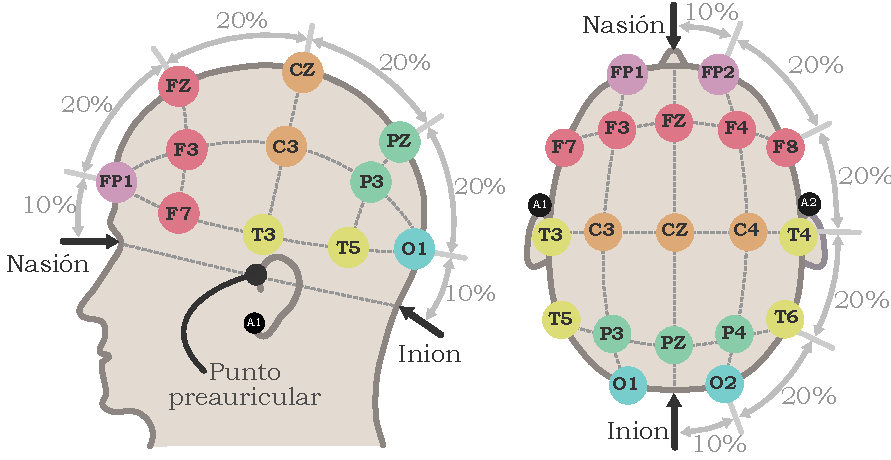
\includegraphics[width=\linewidth]{./img_diagramas/cabeza_proporcionada_color_v4.pdf} 
%\vspace{2em}
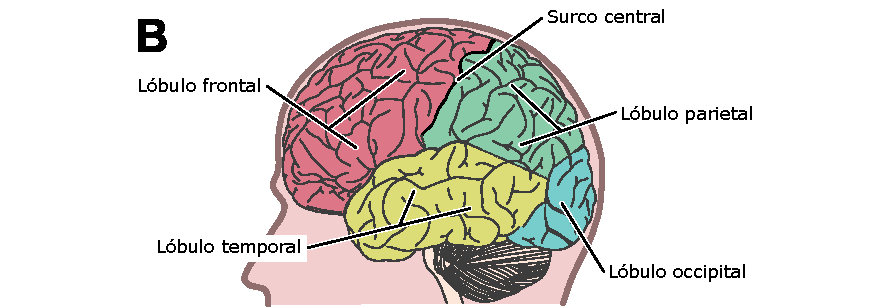
\includegraphics[width=\linewidth]{./img_diagramas/cerebro_1020_v5.pdf} 
\caption[Colocación de electrodos para EEG según el sistema 10--20]{Colocación de electrodos según el sistema 10--20. \textbf{A.} Los electrodos se colocan en una malla de longitudes relativas (medidas en porcentajes) respecto a tres puntos de referencia: inion, nasion, punto preauricular.
\textbf{B.} División de la corteza cerebral en lóbulos, mostrando a grosso modo qué regiones son registradas usando el EEG. Los electrodos del sistema son referidos según los lóbulos cerebrales que \textit{representan}: \underline{F}rontal, \underline{F}ronto\underline{p}olar, \underline{T}emporal, \underline{P}arietal, \underline{O}ccipital. Adicionalmente se registra cerca del surco \underline{C}entral, y los lóbulos \underline{A}uriculares; estos últimos son usados como puntos con actividad eléctrica negligible.
}
\label{img1020}
\end{figure}

Para hablar sobre la forma en que se conectan lo electrodos entre sí, se denota a un par de electrodos como una \textbf{derivación} (también referida como \textit{canal}), mientras que el conjunto de derivaciones es un \textbf{montaje}.
%
En el contexto del presente trabajo se utilizó un montaje \textit{monopolar} (o también llamado \textit{referencial}) en cual se forman las derivaciones conectando en paralelo a cada electrodo con sus respectivos electrodos auriculares cortocircuitados y se usó como tierra a un electrodo colocado en la parte frontal media.

Es importante mencionar que las neuronas en la corteza cerebral tienen orientaciones muy diversas y que disparan de manera asíncrona, de modo que un periodo de gran actividad cerebral bien puede ser visto en el EEG como una actividad desorganizada y de baja amplitud.
%
En otra perspectiva, el cerebro se encuentra cubierto por las capas meninges, por el líquido encefalorraquídeo, el cráneo y el cuero cabelludo; en suma, los campos eléctricos generados en la corteza cerebral son \textit{víctimas} de una gran difusión espacial.
%
Es por ello que las señales captadas por los electrodos deben ser amplificadas analógicamente antes de ser registradas digitalmente.

Un efecto colateral de amplificar la señal es la inclusión de \textbf{ruido}, entendiendo con ello a las señales que son registradas de manera no deseada.
%
Por ejemplo, los músculos faciales generan campos eléctricos con una frecuencia aproximada de 100 \hz; este tipo de ruidos \textit{persistentes} (referido como \textit{ruido de fondo}) son eliminados usando filtros de banda.
%
En contraparte, los ruidos esporádicos de corta duración, típicamente son señalados \textit{a mano} y provocan que el segmento de registro sea invalidado; por ejemplo, el deslizamiento de un electrodo sobre el cuero cabelludo.

Como comentario, cabe mencionar que el término EEG suele usarse independientemente de la cantidad y posición de electrodos usados para el registro: se pueden usar sólo algunas derivaciones del sistema 10--20, se pueden hacer cambios como el uso de la nariz como referencia neutral, o se pueden añadir más electrodos como en el sistema 10--10 \cite{Klem99}. 

%%%%%%%%%%%%%%%%%%%%%%%%%%%%%%%%%%%%%%%%%%%%%%%%%%%%%%%%%%%%%%%%%%%%%%%%%%%%%%%%%%%%%%%%%%%%%%%%%%%
%%%%%%%%%%%%%%%%%%%%%%%%%%%%%%%%%%%%%%%%%%%%%%%%%%%%%%%%%%%%%%%%%%%%%%%%%%%%%%%%%%%%%%%%%%%%%%%%%%%

\subsection{Polisomnografía}
\label{sec:emg_eog}

La técnica de PSG consiste en el registro simultáneo durante el sueño de múltiples variables \textit{variables fisiológicas} como respiración, ritmo cardíaco, temperatura, entre otros.
%
La decisión sobre las señales que componen la PSG depende del problema específico que será estudiado.
%
Para ayudar en la clasificación de etapas de sueño, en el contexto del presente trabajo se usó una PSG con registros de actividad ocular, tono muscular y actividad cerebral (EEG).

La actividad ocular es registrada usando la electrooculografía (EOG), una técnica que explota el comportamiento del ojo como un dipolo cuyos polos son la retina y la pupila; los movimientos del ojo inducen variaciones en el campo eléctricos generados por los electrodos de registro.
%
El registro del EOG incluye una derivación para cada ojo, LOG y ROG, conectado con el electrodo auricular cortocircuitado.
%
Así como con el EEG, la ubicación de los electrodos para EOG se indica en la figura \ref{emg_eog}.
%
Cabe mencionar que el registro de EOG debe ser interpretado como el movimiento del ojo, proyectado sobre el eje formado por los electrodos de registro.

El tono muscular es vigilado usando la técnica de electromiografía (EMG), la cual \textit{observa} la actividad eléctrica producida por las fibras musculares.
%
Su registro contempla una derivación (EMG) con tres electrodos que actúan eléctricamente como tierra, fase y neutro; la ubicación de estos electrodos se indica en la figura \ref{emg_eog}. De forma parecida a esta figura, aunque en los músculos del mentón, en el presente trabajo se colocaron dos electrodos referenciados bipolarmente.  
%
En el contexto del presente trabajo, se espera observar la \textit{casi desaparición} del tono muscular para la detección del sueño MOR.

A modo de comentario, en la figura \ref{ejemplos_mor} se muestra parte de un registro de PSG durante sueño MOR exhibiendo las características descritas previamente.

\begin{figure}
\centering
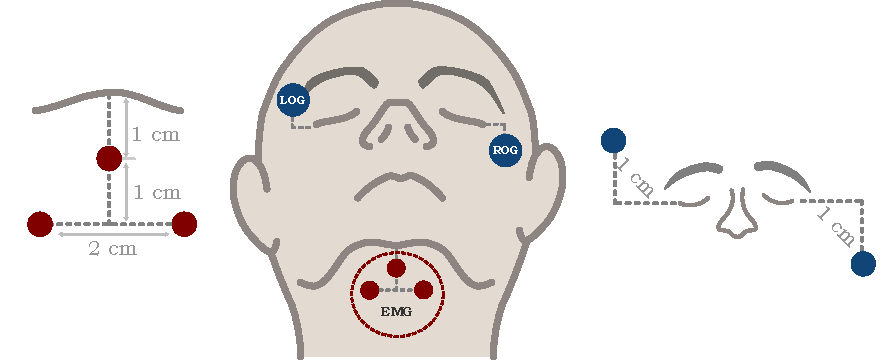
\includegraphics[width=\linewidth]
{./img_diagramas/emg_eog_v4.pdf}
\caption[Colocación de electrodos para electrooculografía y electromiografía]{Colocación de electrodos para el registro de electrooculografía en ambos ojos (LOG, ROG) y electromiografía (EMG). Las líneas punteadas son paralelas al eje medial, y las líneas discontinuas son perpendiculares al mismo. La línea de referencia para EMG inicia en el punto medial en la barbilla.}
\label{emg_eog}
\end{figure}

\begin{figure}
\centering
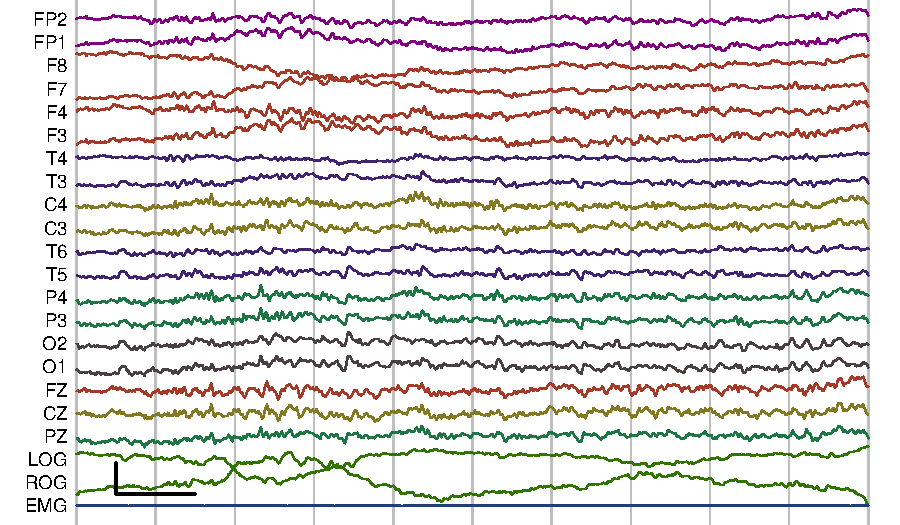
\includegraphics[width=.92\linewidth]
{./img_ejemplos/MJNN_epoca_stam.pdf}
\caption[Registro de polisomnograma durante sueño MOR]
{Registro de PSG durante sueño MOR. En el margen izquierdo se indica la derivación representada; aunque la mayoría corresponden al EEG, en la porción inferior se contempla al EOG y EMG.
%Para más detalles sobre la ubicación de las derivaciones, ver el texto y la figura \ref{emg_eog}. 
Marca de calibración: vertical, 10 \mv, horizontal, 1 segundo.}
\label{ejemplos_mor}
\end{figure}

%%%%%%%%%%%%%%%%%%%%%%%%%%%%%%%%%%%%%%%%%%%%%%%%%%%%%%%%%%%%%%%%%%%%%%%%%%%%%%%%%%%%%%%%%%%%%%%%%%%
%%%%%%%%%%%%%%%%%%%%%%%%%%%%%%%%%%%%%%%%%%%%%%%%%%%%%%%%%%%%%%%%%%%%%%%%%%%%%%%%%%%%%%%%%%%%%%%%%%%

\section{Relación entre deterioro cognitivo y sueño}
\label{sec:pdcl_sueno}

Durante el envejecimiento ocurren diversos cambios fisiológicos y psicológicos que conllevan a modificaciones en el estilo de vida, y particularmente en la rutina de sueño.
%
Hay una vasta cantidad de estudios que han explorado la posible relación entre trastornos del sueño y marcadores \textit{biológicos} de daño neuronal (como la presencia de proteína $\beta$-amiloide, marcador de la enfermedad de Alzheimer) o marcadores de actividad cerebral anómala; la tendencia es considerar que los trastornos del sueño contribuyen en el proceso de deterioro cognitivo, o bien que pueden predecirlo con cierto grado de exactitud \cite{porter15}.

En adultos mayores con DCL durante el sueño MOR se ha reportado una mayor potencia absoluta y relativa en frecuencias lentas para regiones frontales laterales \cite{Brayet16} y una menor atonía muscular \cite{Chen}, respecto a individuos sanos.

Estos resultados concuerdan con el argumento de que tradicionalmente se considera que el sueño MOR desempeña un papel importante en la cognición, particularmente en la consolidación de la memoria \cite{Corsi1983}.
%
Se sabe que los periodos de aprendizaje inducen una mayor duración del sueño MOR y densidad de movimientos oculares rápidos, y también que la privación del sueño MOR se asocia con deficiencias en tareas de memoria \cite{smith96,smith01}.

Se ha propuesto que el mecanismo neurológico asociado a la consolidación de la memoria no es exclusivo del sueño MOR, sino que el conjunto de procesos involucrados se \textit{distribuyen} durante las diferentes etapas del sueño; la porción del proceso ocurrida en sueño MOR corresponde a la \textit{asimilación} de información \cite{diekelmann10}.

Anatómicamente, la consolidación de la memoria está relacionada con el sistema colinérgico\footnote{Circuitos neuronales que usan la acetilcolina como neurotransmisor principal.} en la parte anterior del cerebro \cite{Blake}.
%
Esto es destacable ya que los circuitos colinérgicos son particularmente vulnerables a degradación estructural durante el envejecimiento y sobre todo en presencia de patologías \cite{Schliebs11}.

Por lo tanto, se esperarían diferencias en el grado de estacionariedad entre el sueño MOR y el NMOR, si se sabe que el sueño MOR presenta los característicos movimientos oculares rápidos en contraste con el sueño NMOR en derivaciones relacionadas a los ojos. Además, se exploraron posibles marcadores entre el grupo con PDCL versus el grupo sin PDCL, considerando lo que se mencionó sobre una lentificación de la actividad eléctrica durante el sueño MOR en regiones frontales en los sujetos con PDCL \cite{Brayet16}, ya que, hasta donde se sabe, no se han buscado marcadores como los que se presentan aquí.
%-------------------------------------------------------------------------------
%-------------------------------------------------------------------------------
%Se ha encontrado, por ejemplo, correlaciones entre el DCL en adultos mayores con la \textit{presencia} de ciertos tipos de ondas cerebrales \cite{babiloni13,prichep94,prichep06}.
%
%Se ha reportado una mayor potencia absoluta y relativa en frecuencias lentas para regiones laterales \cite{Brayet16} y una menor atonía muscular \cite{Chen} para adultos mayores con DCL, respecto a individuos sanos.
%-------------------------------------------------------------------------------
%-------------------------------------------------------------------------------

%%%%%%%%%%%%%%%%%%%%%%%%%%%%%%%%%%%%%%%%%%%%%%%%%%%%%%%%%%%%%%%%%%%%%%%%%%%%%%%%%%%%%%%%%%%%%%%%%%%
%%%%%%%%%%%%%%%%%%%%%%%%%%%%%%%%%%%%%%%%%%%%%%%%%%%%%%%%%%%%%%%%%%%%%%%%%%%%%%%%%%%%%%%%%%%%%%%%%%%
%%%%%%%%%%%%%%%%%%%%%%%%%%%%%%%%%%%%%%%%%%%%%%%%%%%%%%%%%%%%%%%%%%%%%%%%%%%%%%%%%%%%%%%%%%%%%%%%%%%
%%%%%%%%%%%%%%%%%%%%%%%%%%%%%%%%%%%%%%%%%%%%%%%%%%%%%%%%%%%%%%%%%%%%%%%%%%%%%%%%%%%%%%%%%%%%%%%%%%%

\chapter{Metodología y resultados}
\label{ch:metodologia}

El presente trabajo surge a partir de una colaboración con el Laboratorio de Sueño, Emoción y Cognición, del Instituto de Ciencias de la Salud (ICSa) de la UAEH a cargo de la Dra. Alejandra Rosales Lagarde.
%
Esta colaboración permitió el acceso a los registros obtenidos en un estudio comenzado por la Dra. Rosales y por Vázquez-Tagle durante los años de 2014 a 2017 \cite{VazquezTagle16}. 
%
Dicha investigación se centró en el estudio del deterioro cognitivo en adultos mayores del estado de Hidalgo, y se consideraron registros de PSG para evaluar parámetros relacionados al sueño y en especial al sueño MOR.
%
El presente trabajo tiene como objetivo particular analizar con mayor detalle dichos registros.

En este capítulo se describe primeramente la metodología seguida para obtener los registros de PSG.
%
Posteriormente se describe la metodología usada para analizar los registros de PSG, usando las herramientas descritas en el capítulo \ref{capitulo:espectro_evo}.

Los registros de PSG fueron segmentados en ventanas de 30 segundos, referidas como \textbf{épocas}.
%
El análisis de los registros de PSG se llevó a cabo a tres niveles:
\begin{itemize}
\item Dentro de cada época.
\item Entre las diferentes épocas en un registro.
\item Entre los diferentes participantes.
\end{itemize}

El análisis a nivel de época contempla su clasificación según etapa de sueño (limitada a MOR y NMOR), y su clasificación como estacionarias o no estacionarias (usando la prueba de PSR).
%
El uso de épocas como unidades de estudio se justifica por la gran heterogeneidad del sueño nocturno; paralelamente, destaca el supuesto fisiológico de que las etapas de sueño son \textit{parecidas} entre los humanos.
%
En suma, los registros de PSG para un sólo individuo pueden interpretarse como una población de épocas.

El análisis a nivel de registro surge de considerar la heterogeneidad del sueño pero usando al registro entero como unidad de estudio.
%
El tomar las épocas junto con su estructura temporal reveló algunos patrones interesantes de actividad.

Para el análisis entre participantes (divididos en grupos), varias de las características descritas fueron \textit{colapsadas} para constituir características \textit{simples}. 
%
Debido a las características de la muestra (ver más adelante), los resultados obtenidos no pueden extrapolarse a la población en general.
%
Los resultados obtenidos, entonces, se presentan como \textit{indicios}.

Los resultados en los tres tipos de análisis fueron repetidos usando la clasificación de estacionariedad obtenida para diferentes tamaños de ventana.
%
Bajo el supuesto de estacionariedad local es, en principio, posible que la estimación de varias características se vea afectada por el tamaño de ventana utilizado; este efecto es cualitativamente diferente que el de la cantidad de puntos considerados.
%
Para mayor información sobre el efecto esperado por la estacionariedad local, ver sección \ref{sec:est_local}.

%%%%%%%%%%%%%%%%%%%%%%%%%%%%%%%%%%%%%%%%%%%%%%%%%%%%%%%%%%%%%%%%%%%%%%%%%%%%%%%%%%%%%%%%%%%%%%%%%%%
%%%%%%%%%%%%%%%%%%%%%%%%%%%%%%%%%%%%%%%%%%%%%%%%%%%%%%%%%%%%%%%%%%%%%%%%%%%%%%%%%%%%%%%%%%%%%%%%%%%

\section{Características de los participantes}

Los participantes fueron elegidos usando un muestreo \textit{no probabilístico por conveniencia} bajo los siguientes criterios de inclusión:
\begin{itemize}
\item Edad entre 60 y 85 años.
\item Diestros (mano derecha dominante).
\item Sin ansiedad, depresión ni síndromes focales.
\item No usar medicamentos o sustancias para dormir.
\item Firma de consentimiento informado.
\item Terminar el estudio de forma voluntaria en lo que corresponde a la aplicación de pruebas y el registro de la PSG.
\end{itemize}

Un total de 16 adultos mayores cumplieron los criterios de inclusión. 
%
Con el fin de detectar el DCL en estos pacientes, éstos fueron sometidos a una batería de pruebas neuropsicológicas para determinar su estado cognoscitivo general (Neuropsi, MMSE), detectar cambios en su vida cotidiana (KATZ) y descartar cuadros ansiosos y depresivos (SAST, GDS); para más detalles ver capítulo anterior, sección \ref{seccion:pruebas}.
%
En la tabla \ref{tab_sujetos} se reportan los puntajes obtenidos por los participantes en dichas pruebas; estos datos deben ser interpretados según los \textit{puntajes de corte} de cada prueba, que se incluyen en el apéndice \ref{apendice_pruebas}.
%
Se determinó que 11 de los voluntarios no padecen depresión o ansiedad, ni presentan afectaciones significativas en la vida diaria; el participante MGG presenta un cuadro depresivo, pero fue incluido en ausencia de afecciones cognitivas objetivas y porque el sueño presentó una arquitectura de sueño normal, de acuerdo a una experta en neurofisiología quien analizó todos los registros. Cabe señalar que los pacientes con depresión suelen tener una latencia al sueño MOR más corta y en esta paciente fue normal.
%
Debido a motivos técnicos, sólo 9 participantes fueron considerados para el presente trabajo; se reportan únicamente los datos relativos a esos participantes.

Con base en el diagnóstico de PDCL, los 9 participantes fueron divididos en dos grupos: PDCL y CTRL. 
%
Es importante mencionar que, bajo las condiciones muestrales, el grupo CTRL no puede fungir satisfactoriamente como grupo control; una descripción más adecuada sería \textit{grupo sin PDCL}.

\begin{table}
\caption{Datos generales de los participantes}
\centering
\bordes{1.1}
{\small
\begin{tabular}{llcrrrrrrr}
\toprule
 \phantom{mmm}&
 & {Sexo} & {Edad} & {Escol.} & {Neuropsi} & {MMSE} & {SAST} & {KATZ} & {GDS} \\
\midrule
\multicolumn{2}{l}{\textbf{Grupo CTRL}}\\
&MJH    & F    & 72\pz & 9\pz  & 113\pz & 30\pz & 18\pz & 0\pz & 0\pz  \\
&JAE    & F    & 78\pz & 5\pz  & 102\pz & 28\pz & 19\pz & 0\pz & 5\pz  \\
&MGG    & F    & 61\pz & 9\pz  & 114\pz & 28\pz & 29\pz & 1\pz & 14\pz \\
&EMT    & F    & 50\pz & 22\pz & 117\pz & 30\pz & 15\pz & 0\pz & 4\pz  \\
\rowcolor{gris}
&\multicolumn{1}{c}{$\widehat{\mu}$} & 
               & 65.3  & 11.3  & 111.5  & 29.0  & 20.3  & 0.3  & 5.8  \\
\rowcolor{gris}
&\multicolumn{1}{c}{$\widehat{\sigma}$} & 
               & 12.4  & 7.4   & 6.6    & 1.2   & 6.1   & 0.5  & 5.9  \\
\midrulec
%\hline
\multicolumn{2}{l}{\textbf{Grupo PDCL}}\\
& CLO   & F    & 68\pz &  5\pz &  81\pz & 28\pz & 22\pz & 1\pz &  6\pz \\
& RLO   & F    & 63\pz &  9\pz &  90\pz & 29\pz & 20\pz & 0\pz &  3\pz \\
& JGZ   & M    & 65\pz & 11\pz &  87\pz & 25\pz & 20\pz & 0\pz &  1\pz \\
& AEFP  & M    & 73\pz &  8\pz &  96\pz & 29\pz &   \pz & 0\pz &  2\pz \\
& PCM   & M    & 71\pz &  9\pz & 111\pz & 28\pz & 20\pz & 0\pz & 10\pz \\
\rowcolor{gris}
&\multicolumn{1}{c}{$\widehat{\mu}$} & 
              &  68.0  & 8.4   & 93.0   & 27.8  & 20.5  & 0.2  & 4.4  \\
\rowcolor{gris}
&\multicolumn{1}{c}{$\widehat{\sigma}$} & 
              & 4.1    & 2.2   & 11.4   & 1.6   & 1.0   & 0.4  & 3.6 \\
\bottomrulec
\end{tabular} 
}
\label{tab_sujetos}
\end{table}

%%%%%%%%%%%%%%%%%%%%%%%%%%%%%%%%%%%%%%%%%%%%%%%%%%%%%%%%%%%%%%%%%%%%%%%%%%%%%%%%%%%%%%%%%%%%%%%%%%%
%%%%%%%%%%%%%%%%%%%%%%%%%%%%%%%%%%%%%%%%%%%%%%%%%%%%%%%%%%%%%%%%%%%%%%%%%%%%%%%%%%%%%%%%%%%%%%%%%%%

\subsection{Registro del polisomnograma}

Para efectuar el registro de la PSG, los participantes acudieron a las instalaciones del Laboratorio de Sueño, Emoción y Cognición en el ICSa. 
%
Los participantes recibieron instrucciones de realizar una rutina normal de actividades durante la semana que precedió al estudio, y se les recomendó no ingerir bebidas alcohólicas o energizantes (como café o refresco) durante las 24 horas previas al experimento, y que no durmieran siesta ese día.
%
Bajo estas condiciones experimentales se garantiza que los registros son representativos del sueño nocturno de cada participante.

El registro per se fue efectuado usando un polisomnógrafo Medicid 5 (Neuronic Mexicana). El montaje de la PSG incluyó los siguientes electrodos\footnote{Para más detalles ver el capítulo anterior, particularmente la sección \ref{capitulo:psg}}:
\begin{itemize}
\item 19 electrodos de EEG colocadas según el Sistema Internacional 10--20.
\item 2 electrodos de EOG para movimientos oculares.
\item 2 electrodos de EMG para medir el tono muscular en los músculos del mentón.
\end{itemize}

Los electrodos para EEG fueron conectados en paralelo usando como referencias los lóbulos de las orejas cortocircuitadas; la impedancia se mantuvo por debajo de \SI{50}{\micro\ohm}.
%
Las señales fueron amplificadas analógicamente usando amplificadores de alta ganancia en cadena, y adicionalmente fueron \textit{pasados por} filtros analógicos pasa bandas: 0.1--100 Hz para EEG, 3--20 Hz para EOG. 
%
Los registros fueron digitalizados con una frecuencia de muestreo de 512 puntos por segundo (Hz), y posteriormente almacenados en formato de texto.

Como se mencionó anteriormente, los registros fueron segmentados en 30 segundos, referidos como \textbf{épocas}, por lo que a partir de este momento se usará la palabra `época' como un caso particular de la ventana.
%
Cada una de las épocas fue clasificada como MOR o NMOR; la clasificación fue llevada a cabo por dos expertos del ICSA y una neurofisióloga de la UNAM, y bajo los estándares de la AASM.

Por simplicidad técnica, los registros fueron truncados para poder considerar épocas completas; algunos datos al final de cada registro fueron omitidos, aunque representan una cantidad negligible de tiempo.
%
Cabe mencionar que cada época de 30 segundos, a una frecuencia de 512 Hz, representa un total de 15,360 puntos.

En la tabla \ref{tab:psg} se describe la duración de los registros, así como la cantidad de tiempo del registro clasificado como sueño MOR.
%
La cantidad de tiempo en vigilia registrado es negligible ($<5$ minutos por cada participante), de modo que ésta no es reportada; con una pérdida mínima de generalidad, se puede afirmar que los registros fuera del sueño MOR corresponden a sueño NMOR.

\begin{table}
\centering
\caption{Datos generales sobre los registros de PSG}
\bordes{1.2}
\begin{tabular}{lllrclrr}
\toprule
    \phantom{mmm}&
    & \multicolumn{2}{l}{TTS} & \phantom{l}   & \multicolumn{3}{l}{MOR*}\\
    \cmidrule{3-4}  \cmidrule{6-8}
    &          &Épocas  &  Min.   &&Épocas  &  Min.   &  \% \\
\midrule
\multicolumn{2}{l}{\textbf{Grupo CTL}}\\
&MJH &    1032   &  516\pz && 127    & 63.5  &12.31 \\
&JAE &\ppu 904   &  452\pz && 171    & 85.5  &18.92 \\
&MGG &    1024   &  512\pz && 166    & 83\pz &16.21 \\
&EMT &\ppu 552   &  276\pz &&  47    & 23.5  & 8.51 \\
 
\rowcolor{gris}
&\multicolumn{1}{c}{$\widehat{\mu}$}  
     &\ppu 878.0 &  439.0  && 128.0  & 63.9  &13.99 \\
\rowcolor{gris}
&\multicolumn{1}{c}{$\widehat{\sigma}$} 
     &\ppu 225.1 &  112.5  &&  57.3  & 28.7  &4.55 \\ 
\midrulec

\multicolumn{2}{l}{\textbf{Grupo PDC}}\\
&CLO  &\ppu 944   & 472\pz && 132\pz & 66\pz & 13.98 \\
&RLO  &\ppu 840   & 420\pz &&  99\pz & 49.5  & 11.79 \\
&JGZ  &    1200   & 600\pz &&  34\pz & 17\pz &  2.83 \\
&AEFP &\ppu 952   & 476\pz &&  41\pz & 20.5  &  4.31 \\
&PCM  &\ppu 752   & 376\pz &&  59\pz & 29.5  &  7.85 \\
 
\rowcolor{gris}
&\multicolumn{1}{c}{$\widehat{\mu}$}  
      &\ppu 937.6 & 468.8 &&   73.0  & 36.5  & 8.15 \\
\rowcolor{gris}
&\multicolumn{1}{c}{$\widehat{\sigma}$} 
      &\ppu 168.1 &  84.1 &&   41.5  & 20.8  & 4.75 \\
\bottomrulec
\end{tabular} \\
\begin{small}
\begin{tabular}{l}
{*El sueño MOR aparece fragmentado, se reporta la suma de tales tiempos.}\\
{TTS= Tiempo Total de sueño.} {El porcentaje de sueño MOR se calcula respecto al TTS.}
\end{tabular}
\end{small}
\label{tab:psg}
\end{table}

%%%%%%%%%%%%%%%%%%%%%%%%%%%%%%%%%%%%%%%%%%%%%%%%%%%%%%%%%%%%%%%%%%%%%%%%%%%%%%%%%%%%%%%%%%%%%%%%%%%
%%%%%%%%%%%%%%%%%%%%%%%%%%%%%%%%%%%%%%%%%%%%%%%%%%%%%%%%%%%%%%%%%%%%%%%%%%%%%%%%%%%%%%%%%%%%%%%%%%%

\section{Características muestrales}

Previo a los análisis de los registros de PSG, se corroboró si los dos grupos de participantes efectivamente se \textit{comportan} como grupos estadísticamente diferentes.
%
Con dicho objetivo, se aplicaron pruebas $U$ de Wilcoxon-Mann-Whithney (WMW) entre los dos grupos, para todas las variables consideradas. 
%
De lo anterior se exceptúa al puntaje de la prueba KATZ, ya que es un parámetro cualitativo. 
%
Se concluye que las mediciones son parecidas en ambos grupos para todas las variables observadas, excepto para el puntaje en la prueba Neuropsi; ello era de esperarse ya que el puntaje en Neuropsi fue usado para designar a los participantes en los grupos.
%
Los resultados de estas pruebas se reportan en la tabla \ref{tab:var_wilcox}.

\begin{table}
\centering
\caption{Variables independientes entre grupos}
\begin{tabular}{lrlcrlccr}
\toprule
 & \multicolumn{2}{l}{Grupo CTRL} & \phantom{.} & \multicolumn{2}{l}{Grupo PDCL} 
 & \phantom{.} & \multicolumn{2}{l}{WMW}
 \\
\cmidrule{2-3} \cmidrule{5-6} \cmidrule{8-9}
            & Media & (DE)  & & Media & (DE) & & $p$ & $W$ \\
\midrule
Edad        &  65.3 &  12.4 & &  68.0 &  4.1 & &    0.905 &  9.0  \\
Escolaridad &  11.3 &   7.4 & &   8.4 &  2.2 & &    0.797 & 11.5 \\
Neuropsi    & 111.5 &   6.6 & &  93.0 & 11.4 & &\bf 0.032 & 19.0 \\
MMSE        &  29.0 &   1.2 & &  27.8 &  1.6 & &    0.366 & 14.0 \\
SATS        &  20.3 &   6.1 & &  20.5 &  1.0 & &    0.301 &  4.0  \\
GDS         &   5.8 &   5.9 & &   4.4 &  3.6 & &    0.905 & 11.0 \\
TTS [min]   & 439.0 & 112.5 & & 468.8 & 84.2 & &    1.000 & 10.0 \\
MOR [min]   &  63.9 &  28.7 & &  36.5 & 20.8 & &    0.190 & 16.0 \\
MOR [\%]    &  14.0 &   4.5 & &   8.2 &  4.8 & &    0.111 & 17.0 \\
\bottomrule 
\multicolumn{9}{l}{WMW=Prueba de Wilcoxon--Mann--Whitney, DE=Desviación}\\
\multicolumn{9}{l}{Estándar, TTS=Tiempo Total de Sueño.}
\end{tabular} 
\label{tab:var_wilcox}
\end{table}

Se verificó si hay correlaciones entre las variables consideradas, lo cual podría afectar la interpretación de los resultados posteriores.
%
Para ello se aplicó la prueba de correlación de Spearman a cada par de variables; la prueba de Spearman estima la correlación entre variables, y se prueba la hipótesis de que la correlación es diferente de cero.
%
Estos resultados se reportan en el cuadro \ref{tab:correlacion}.

\begin{table}
\centering
\caption{Prueba de correlación de Spearman (estimación y p-valor)}
\begin{tabular}{lcccccccc}
\toprule
             & \rotatebox{80}{Escolaridad} & \rotatebox{80}{Neuropsi} & \rotatebox{80}{MMSE} & \rotatebox{80}{SAST} & \rotatebox{80}{GDS} & \rotatebox{80}{Sueño [min]} & \rotatebox{80}{MOR [min]} & \rotatebox{80}{MOR [\%]} \\
\midrule
Edad        & -0.699 & -0.267 & -0.079 & -0.171 & -0.233 & 0.200  & 0.183  & 0.100   \\
            & (\textbf{0.04}) & (0.49) & (0.84) & (0.69) & (0.55) & (0.61) & (0.64) & (0.81)  \\
\rowcolor{gris}
Escol.      &        & 0.437  & 0.194  & -0.366 & -0.254 & -0.044 & -0.586 & -0.525  \\
\rowcolor{gris}
            &        & (0.24) & (0.62) & (0.37) & (0.51) & (0.91) & (0.10) & (0.15)  \\

Neuropsi    &        &        & 0.501  & -0.415 & 0.200  & -0.267 & 0.150  & 0.200   \\
            &        &        & (0.17) & (0.31) & (0.61) & (0.49) & (0.71) & (0.61)  \\

\rowcolor{gris}
MMSE        &        &        &        & -0.628 & -0.378 & -0.316 & -0.070 & 0.018   \\
\rowcolor{gris}
            &        &        &        & (0.09) & (0.32) & (0.41) & (0.86) & (0.96)  \\

SATS        &        &        &        &        & 0.610  & 0.317  & 0.293  & 0.195   \\
            &        &        &        &        & (0.11) & (0.44) & (0.48) & (0.64)  \\

\rowcolor{gris}
GDS         &        &        &        &        &        & -0.433 & 0.517  & 0.467   \\
\rowcolor{gris}
            &        &        &        &        &        & (0.25) & (0.16) & (0.21)  \\

Sueño [min] &        &        &        &        &        &        & -0.050 & -0.067  \\
            &        &        &        &        &        &        & (0.91) & (0.88)  \\

\rowcolor{gris}
MOR [min]   &        &        &        &        &        &        &        & 0.983   \\
\rowcolor{gris}
            &        &        &        &        &        &        &        & (\textbf{0.00})  \\
\bottomrulec
\end{tabular}
\label{tab:correlacion}
\end{table}

Sólo se encontraron correlaciones significativas entre dos pares de variables: edad y escolaridad, y tiempo en MOR \textit{medido} en segundos y en porcentaje.

La primera relación, no muy fuerte, puede explicarse como un \textit{efecto generacional}: la educación superior ha aumentado su cobertura durante las últimas décadas, y entonces los grupos poblacionales más jóvenes tienen en promedio más años de escolaridad. 
%
Una segunda hipótesis para esta correlación es la contribución del participante EMT, quien tiene una edad menor y un nivel de educación mayor al resto de los participantes.
%
Para contrastar la segunda hipótesis se calculó nuevamente la prueba de Spearman pero retirando los datos de EMT: se halló una correlación estimada de 0.179 con un p-valor asociado de 0.672, que no permite rechazar el que la correlación sea diferente de cero.

Se descarta entonces la hipótesis del efecto generacional, cuando menos para el grupo de participantes considerados, y se acepta que la correlación es debida a valores atípicos. Se concluye que, usando los datos recabados, no se puede obtener información relevante sobre el efecto del nivel de educación ni la edad sobre el PDCL, ni con los marcadores del PSG que se describirán más adelante.

Intuitivamente era de esperarse la correlación entre el tiempo en MOR y el porcentaje de sueño que es MOR.
%
Sin embargo, la hipótesis de que el sueño tenga una \textit{estructura característica} --y por tanto, que las etapas de sueño aparezcan en proporciones similares en varios individuos--- es ajena a los supuestos estadísticos.
%
Con base en este resultado, en adelante se usará el porcentaje de MOR como \textit{sustituto} del tiempo real de MOR porque (1) dichas variables están fuertemente correlacionadas, y (2) porque el porcentaje permite comparar intuitivamente características de registros con duraciones muy diferentes.

%%%%%%%%%%%%%%%%%%%%%%%%%%%%%%%%%%%%%%%%%%%%%%%%%%%%%%%%%%%%%%%%%%%%%%%%%%%%%%%%%%%%%%%%%%%%%%%%%%%
%%%%%%%%%%%%%%%%%%%%%%%%%%%%%%%%%%%%%%%%%%%%%%%%%%%%%%%%%%%%%%%%%%%%%%%%%%%%%%%%%%%%%%%%%%%%%%%%%%%

\section{Análisis a nivel de época}
\label{sec:analisis_epoca}

Como se mencionó anteriormente, los registros fueron fragmentados en ventanas de 30 segundos para su clasificación en las etapas de sueño, referidas como épocas.
%
De manera independiente, cada una de estas épocas fue sometida a la prueba de estacionariedad de Priestley--Subba Rao (PSR) para investigar si es estacionaria en el sentido de homogeneidad espectral; para más detalles ver la sección \ref{sec:psr}.

Con base en la prueba de PSR, cada una de las épocas consideradas fue clasificada como \textit{estacionaria} si fue rechazada la hipótesis de no--estacionariedad con un nivel de significancia $p<0.05$.
%
La aplicación per se de la prueba de PSR fue efectuada usando el software estadístico R; en particular, se utilizó la implementación incluida en el paquete \texttt{fractal} bajo la función \texttt{stationarity} \cite{R_fractal}.

Con cada época clasificada según etapa de sueño (MOR o NMOR) y según su estacionariedad, se procedió primeramente a revisar cómo están relacionadas ambas características.
%
Para ello se planteó la hipótesis de que la cantidad de épocas estacionarias es diferente en MOR y NMOR. 

Debido a que la cantidad de épocas en NMOR es considerablemente mayor a las épocas en MOR, y con base en las observaciones de la sección anterior, se usaron proporciones en lugar del total de épocas.
%
Para simplificar la notación, las proporciones de épocas clasificadas como estacionarias en MOR y NMOR serán referidas como $\text{p}_{\text{MOR}}$ y $\text{p}_{\text{NMOR}}$, respectivamente; es decir
\begin{equation}
\text{p}_{\text{MOR}} = \frac{\text{\# épocas estacionarias en MOR}}{\text{\# épocas en MOR}}
\end{equation}
y similarmente para $\text{p}_{\text{NMOR}}$.
%
Dado que las clasificaciones según etapa de sueño (MOR/NMOR) y estacionariedad (sí/no) son dicotómicas, la hipótesis $\text{p}_{\text{MOR}}\neq\text{p}_{\text{NMOR}}$ fue probada usando la prueba $\chi^{2}$ de Pearson; dicha prueba fue repetida para todas las derivaciones consideradas.

Los resultados obtenidos se reportan en el apéndice \ref{apendiceA}, y en la figura \ref{cabeza_new} se muestra de forma esquemática en qué derivaciones se encontraron diferencias significativas.

\begin{figure}
\centering
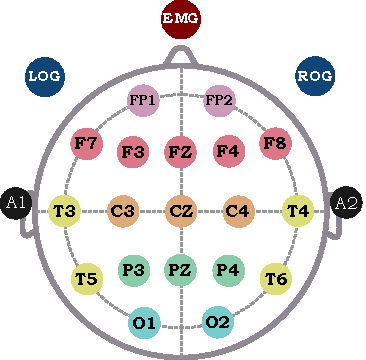
\includegraphics[scale=1.2]
{./img_diagramas/estampa_v1.pdf}
\caption[Representación minimalista de los electrodos para PSG]{Representación minimalista de los electrodos considerados en el registro de PSG;
%: 19 para el EEG, dos para el EOG, un grupo de 3 para el EMG y dos electrodos de referencia.
para más detalles ver las secciones \ref{sec:eeg} y \ref{sec:emg_eog}.
Esta forma de ordenar las gráficas será usada en gráficos posteriores.}
\label{img:estampa}
\end{figure}

\begin{figure}
\centering
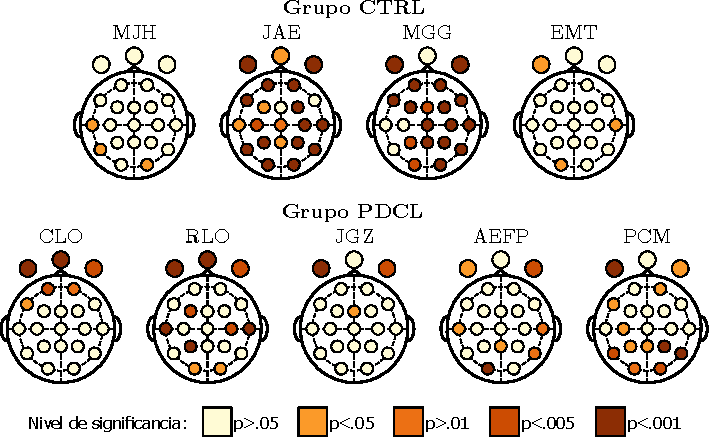
\includegraphics[width=\textwidth]{./img_art_dfa/prop_tabla.pdf} \\
\caption{Derivaciones para las cuales la proporción de épocas clasificadas como estacionarias de acuerdo a la prueba de Priestley-Subba Rao fue significativamente diferente durante el sueño MOR y NMOR.
%
En la parte superior se representa al grupo CTRL y en la parte inferior al grupo con PDCL.
%
Para esta figura se usaron épocas de 30 segundos de duración.
%
La posición de los círculos representa a las derivaciones, en correspondencia con la figura \ref{img:estampa}.}
\label{cabeza_new}
\end{figure}

%%%%%%%%%%%%%%%%%%%%%%%%%%%%%%%%%%%%%%%%%%%%%%%%%%%%%%%%%%%%%%%%%%%%%%%%%%%%%%%%%%%%%%%%%%%%%%%%%%%
%%%%%%%%%%%%%%%%%%%%%%%%%%%%%%%%%%%%%%%%%%%%%%%%%%%%%%%%%%%%%%%%%%%%%%%%%%%%%%%%%%%%%%%%%%%%%%%%%%%

\subsection*{Efecto de la estacionariedad local}

Se procedió a repetir la clasificación de estacionariedad pero usando ventanas de diferentes tamaños.
%
Los tamaños de ventana se eligieron de la forma $30 \times 2^{n}$ segundos por \textit{compatibilidad}, ya que el protocolo de la AASM sugiere usar épocas de 30 segundos para identificar el sueño MOR y por motivos técnicos.
%
El tamaño de ventana más pequeño fue de $\nicefrac{30}{32}$ segundos para poder utilizar la prueba de PSR de forma confiable, mientras que el tamaño más grande fue de $120$ segundos tomando en cuenta que ventanas más grandes serían demasiado heterogéneas para considerarse como unidades de estudio fiables.

En la figura \ref{cabeza_repoio} se muestran únicamente las proporciones estimadas de épocas estacionarias para MOR y NMOR ($\text{p}_{\text{MOR}}$ y $\text{p}_{\text{NMOR}}$) para un participante; los gráficos construidos para todos los participantes pueden encontrarse en el apéndice \ref{apendiceA}.
%
Usando épocas de mayor duración, se encuentra que una proporción menor de éstas son clasificadas como estacionarias; sin embargo, usar épocas de menor duración no garantiza el efecto contrario.
%
Dicho fenómeno \textit{apoya} la hipótesis de estacionariedad local en los registros de PSG en adultos mayores, aunque no representa evidencia suficiente para relacionarlo con el PDCL.

\begin{figure}
\centering
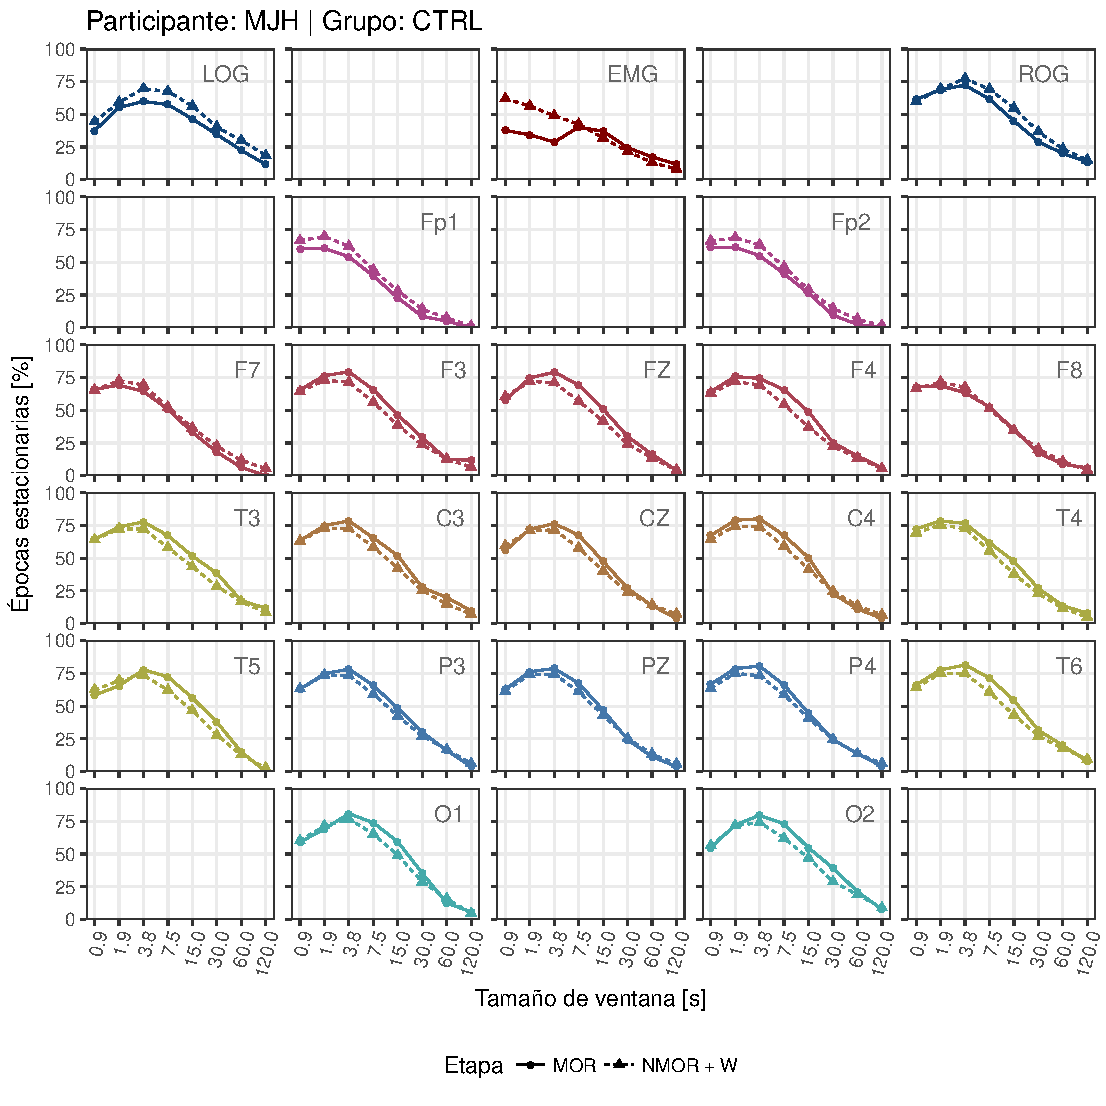
\includegraphics[width=\linewidth]{./scripts_graf_res/MJNNVIGILOS_cabeza_epocas_v2.pdf}
\caption{Cambio en la proporción de épocas estacionarias respecto al tamaño de ventana usado, durante MOR y NMOR. El análisis se repite en todas las derivaciones consideradas; la posición y color de cada gráfico se corresponden a aquellos de la figura \ref{img:estampa}. W = vigilia, recordando que la cantidad de tiempo de los registros clasificada como vigilia es negligible.}
\label{cabeza_repoio}
\end{figure}

En resumen, no se pudo identificar una conexión clara entre el PDCL y las características de las épocas como unidades autónomas.
%
Debido a ello se consideran otros niveles de organización sobre los registros: los registros como un conjunto de épocas distribuidas en el tiempo con \textit{cierta estructura}, y al individuo como unidad en la variabilidad de dichas estructuras.
%
En particular sobre el último, si se supone que las cantidades descritas en esta sección son características \textit{representativas} de cada participante, entonces tiene sentido intentar verificar similitudes con otros participantes o correlaciones con otras observaciones.

%%%%%%%%%%%%%%%%%%%%%%%%%%%%%%%%%%%%%%%%%%%%%%%%%%%%%%%%%%%%%%%%%%%%%%%%%%%%%%%%%%%%%%%%%%%%%%%%%%%
%%%%%%%%%%%%%%%%%%%%%%%%%%%%%%%%%%%%%%%%%%%%%%%%%%%%%%%%%%%%%%%%%%%%%%%%%%%%%%%%%%%%%%%%%%%%%%%%%%%

\section{Análisis a nivel de registro}
\label{sec:analisis_registro}

Con el fin de explorar cómo se relacionan las épocas estacionarias con la \textit{estructura del sueño}, se procedió a \textit{graficar} la estacionariedad.
%
Para efectuar lo anterior se consideró una cuadrícula, con una fila por cada derivación y una columna por cada época analizada (se registró el mismo número de épocas para cada derivación); sobre la cuadrícula el espacio correspondiente a cada época fue coloreado  según la clasificación de la época como estacionaria.
%
Se procedió similarmente para ilustrar la clasificación según la etapa de sueño.
%
En la figura \ref{img:patrones} se ejemplifica este tipo de gráficos, además de otros detalles a mencionarse.

\begin{figure}
\centering
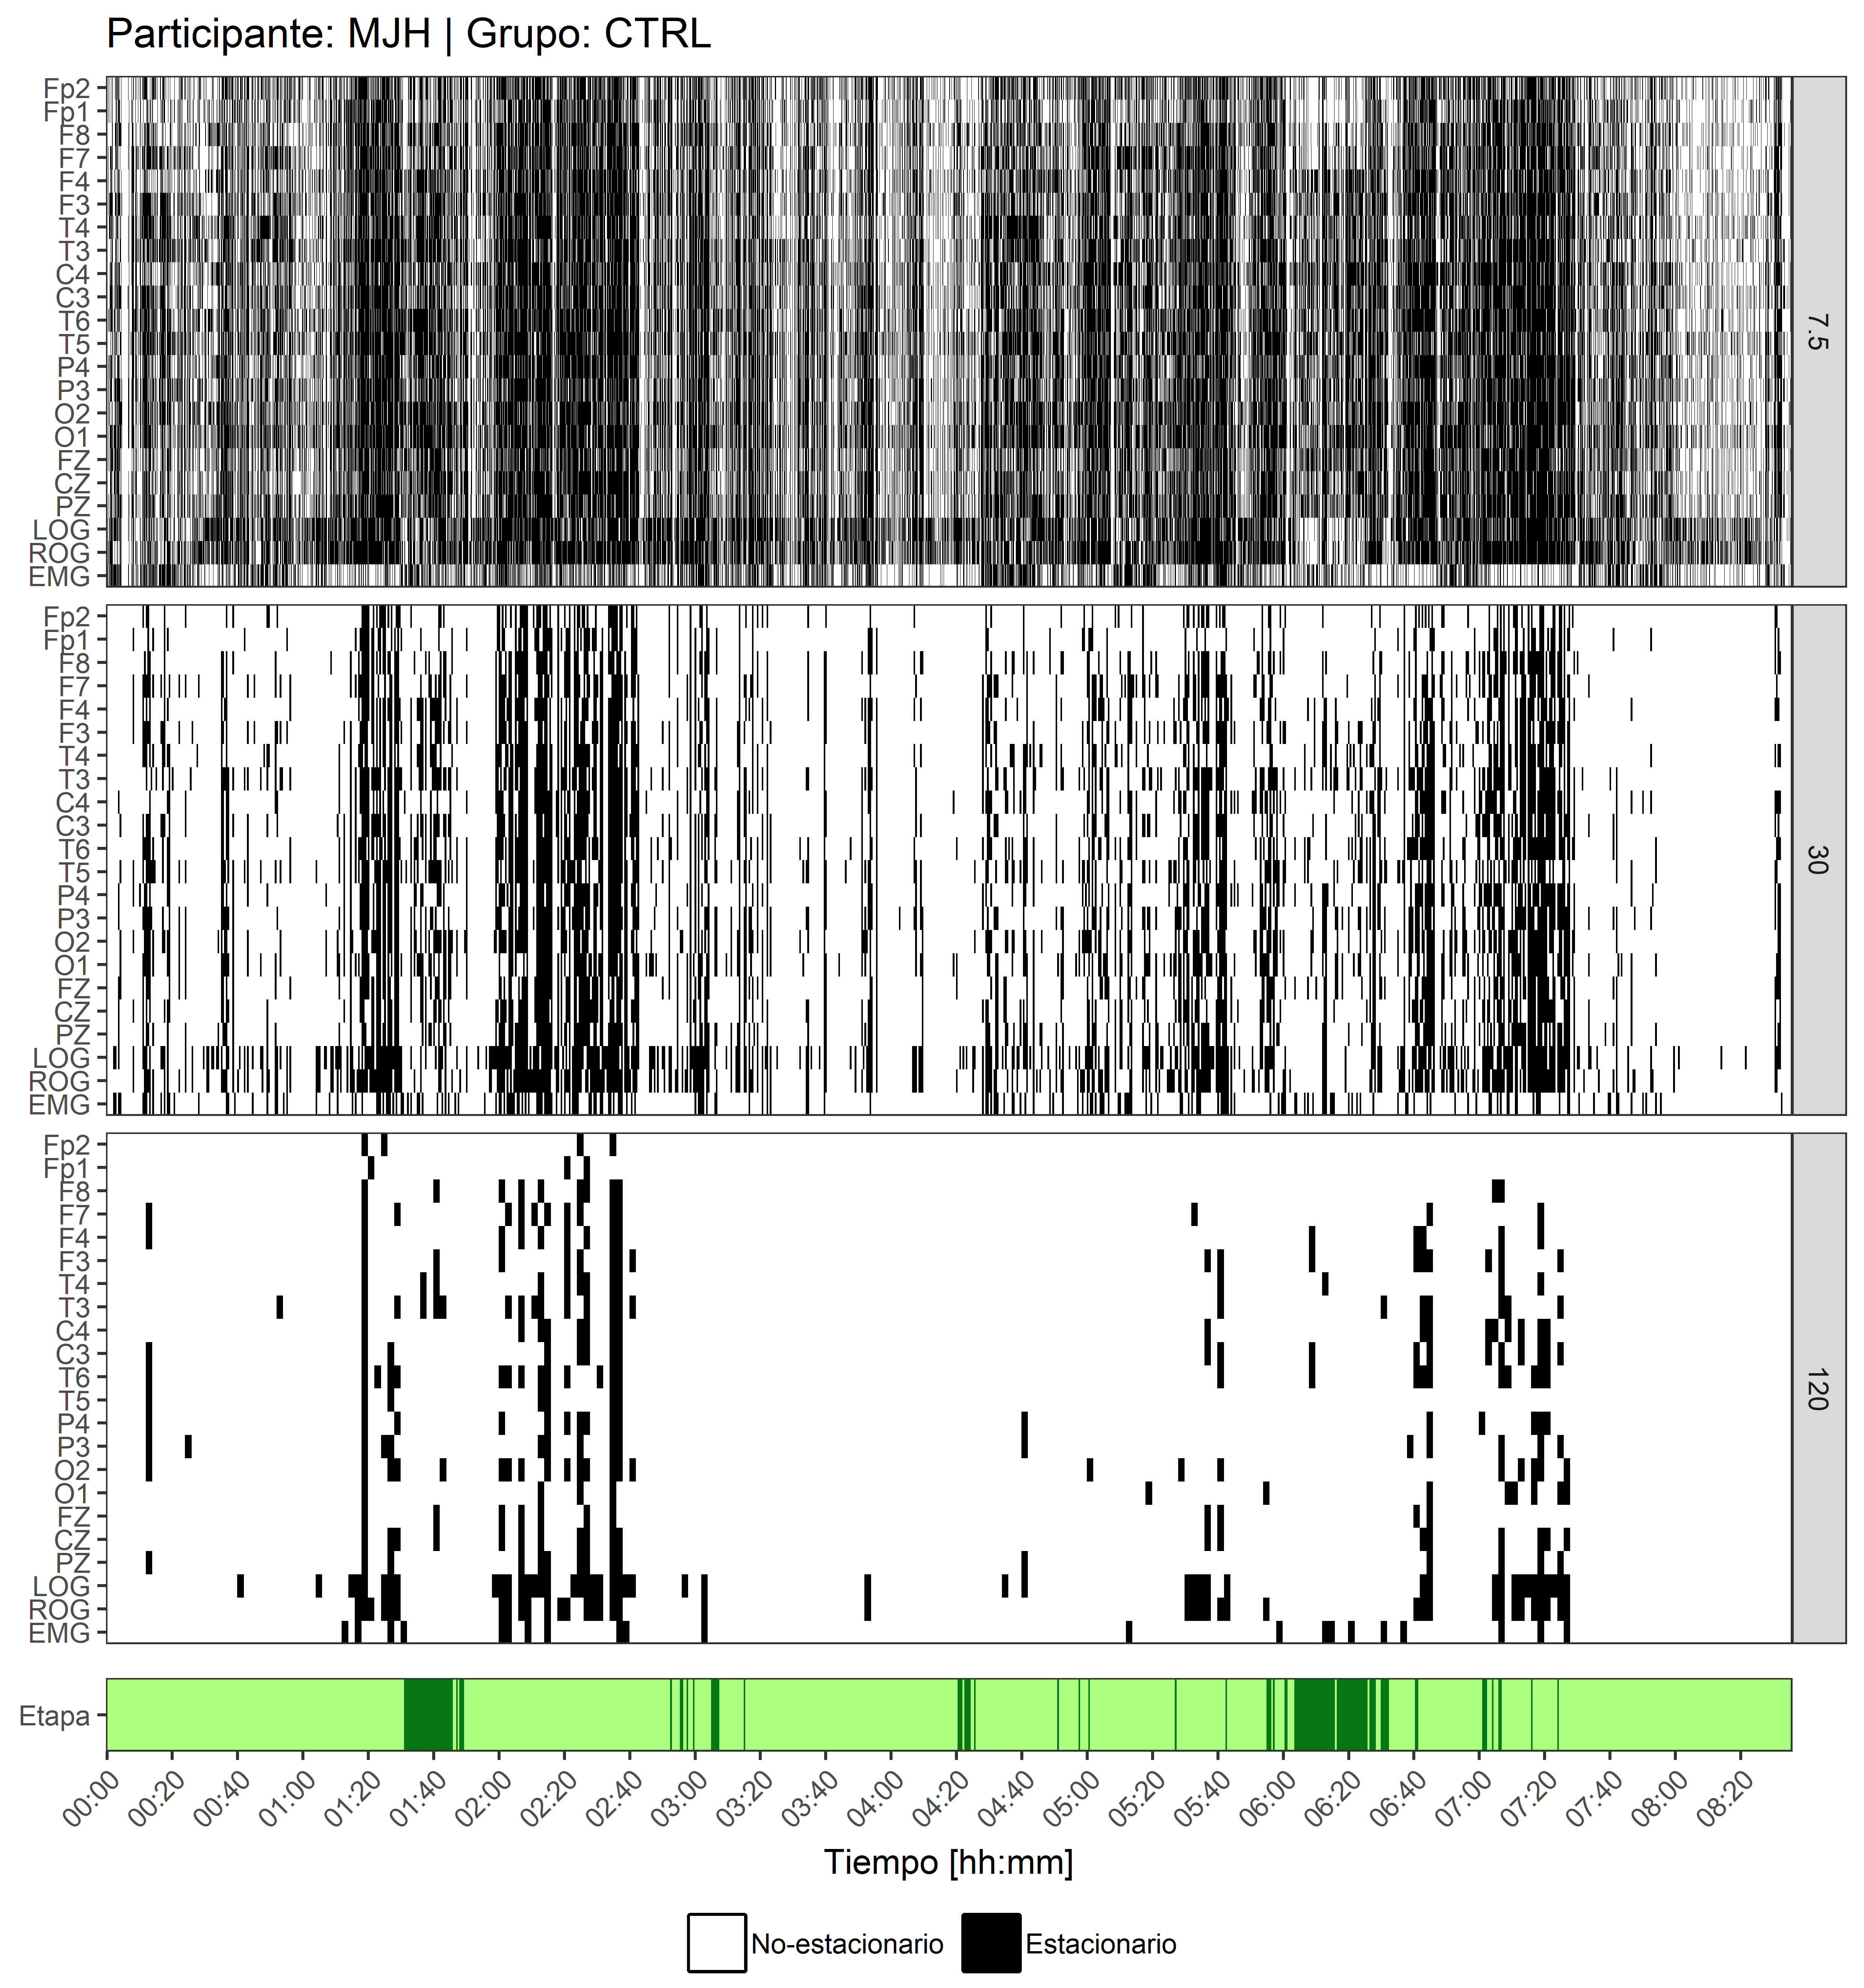
\includegraphics[width=\linewidth]
{./scripts_graf_res/MJNNVIGILOS_patrones_show.png}
\caption[Distribución en el tiempo de las ventanas clasificadas como estacionarias, considerando diferentes tamaños de ventana]{Distribución en el tiempo de las ventanas clasificadas como estacionarias, considerando diferentes tamaños de ventana. 
Cada ventana fue representada en una cuadrícula según su derivación (margen izquierdo) y momento (margen inferior) de procedencia; posteriormente fue \textit{coloreada} según su clasificación como estacionaria.
Dado que la clasificación de estacionariedad se repitió usando diversos tamaños de ventana, en el margen derecho se indica el tamaño de la ventana en segundos.
En la parte inferior se representan las mismas épocas en su clasificación según etapa de sueño.
%Adicionalmente, en la parte superior se indican los \textit{patrones emergentes} de estacionariedad; para más detalles al respecto, ver el texto.
}
\label{img:patrones}
\end{figure}

Los gráficos obtenidos mediante este procedimiento mostraron algunas regularidades que merecen especial atención: \textit{bloques emergentes} de épocas que comparten clasificación como estacionarias (o como no--estacionarias).
%
Estos bloques identificados visualmente se extienden entre diversas derivaciones; puede verse un ejemplo de ello en la figura \ref{img:patrones}.
%
Debido a la forma en que se efectuó la clasificación de estacionariedad (usando la prueba de PSR) puede garantizarse que estos patrones emergentes no son producidos por la clasificación per se.
%
Se hipotetiza que estos \textit{patrones de estacionariedad}
corresponden a las diferentes etapas de sueño.

Dentro del contexto del PDCL en adultos mayores, estos patrones de estacionariedad no serán definidos formalmente ni estudiados detalladamente; se presentan como un hallazgo incidental y como verificación empírica de las capacidades de la técnica descrita para distinguir características que varían en el tiempo.

%%%%%%%%%%%%%%%%%%%%%%%%%%%%%%%%%%%%%%%%%%%%%%%%%%%%%%%%%%%%%%%%%%%%%%%%%%%%%%%%%%%%%%%%%%%%%%%%%%%
%%%%%%%%%%%%%%%%%%%%%%%%%%%%%%%%%%%%%%%%%%%%%%%%%%%%%%%%%%%%%%%%%%%%%%%%%%%%%%%%%%%%%%%%%%%%%%%%%%%

\subsection*{Efecto de la estacionariedad local}

El procedimiento de graficación se repitió para las clasificaciones de estacionariedad obtenidas usando diferentes tamaños de ventana, con el fin de verificar si la presencia de los bloques podría atribuirse al tamaño de ventana usado.
%
Se encontró que los patrones aparecen con mayor o menor \textit{nitidez} en los gráficos obtenidos usando diferentes tamaños de ventana, tal como se ilustra en la figura \ref{img:patrones}.

%%%%%%%%%%%%%%%%%%%%%%%%%%%%%%%%%%%%%%%%%%%%%%%%%%%%%%%%%%%%%%%%%%%%%%%%%%%%%%%%%%%%%%%%%%%%%%%%%%%
%%%%%%%%%%%%%%%%%%%%%%%%%%%%%%%%%%%%%%%%%%%%%%%%%%%%%%%%%%%%%%%%%%%%%%%%%%%%%%%%%%%%%%%%%%%%%%%%%%%

\section{Análisis a nivel de grupo}

Para fines de esta subsección, se ha supuesto que las proporciones de épocas estacionarias durante MOR y NMOR ($\text{p}_{\text{MOR}}$ y $\text{p}_{\text{NMOR}}$) son características intrínsecas de cada individuo. 
%
En otras palabras, si se repite el registro de PSG para el mismo individuo y bajo condiciones similares, y se realiza el mismo procedimiento de segmentación y clasificación de épocas, entonces se espera que las cantidades $\text{p}_{\text{MOR}}$ y $\text{p}_{\text{NMOR}}$ serán las mismas.
%
Este supuesto se basa en que las fases de sueño son \textit{casi indistinguibles} entre diferentes individuos con características similares, y más aún entre diferentes jornadas de sueño para el mismo individuo.

Con base en los resultados de la subsección anterior, se puede afirmar intuitivamente que la metodología descrita \textit{percibe} parte de algunas fases (o subfases) de sueño, las cuales son comunes entre individuos.
%
Sin embargo, aun si tales observaciones fueran verificadas rigurosamente, el supuesto de que $\text{p}_{\text{MOR}}$ y $\text{p}_{\text{NMOR}}$ son características individuales debería ser verificado por separado.
%
Debido a las limitaciones del presente trabajo --especialmente el tamaño muestral reducido y la limitación de un registro por participante-- el supuesto será usado como tal, y no se verificará debido a la falta de datos.
%
En consecuencia, los resultados en la presente subsección se presentan como \textit{indicios}, con la idea de explorarlos en trabajos futuros.

Entonces bien, las cantidades $\text{p}_{\text{MOR}}$ y $\text{p}_{\text{NMOR}}$, calculadas por separado para todos los participantes y todas las derivaciones consideradas, fueron tratados como características que se distribuyen de forma aproximadamente normal sobre las poblaciones que representan los grupos CTRL y PDCL.
%
Se efectuó un ANOVA de dos vías para observar los cambios sobre $\text{p}_{\text{MOR}}$ y $\text{p}_{\text{NMOR}}$ debidos al grupo y la etapa de sueño, cuyos resultados se muestran en el cuadro \ref{tabla:anova_prop}.
%
Se encontró que no hay interacciones significativas entre los factores de etapa y grupo para ninguna derivación; así mismo se encontró que hay diferencias significativas para las derivaciones Fp2, F7, LOG y ROG que pueden ser explicadas por el \textit{efecto} de la etapa se sueño, y de forma similar para las derivaciones LOG y ROG con el efecto de `grupo'.

Las diferencias para LOG y ROG, debidas al efecto de `etapa de sueño', puede explicarse perfectamente por la presencia característica de movimientos oculares rápidos en el sueño MOR. 
%
Este resultado es consistente con una de las tres características que determinan al sueño MOR: atonía muscular, movimientos oculares rápidos y actividad en el EEG de amplitud baja y frecuencias mixtas.
%
Paralelamente estos resultados sugieren que este procedimiento podría ser usado para identificar de forma objetiva y automatizada al sueño MOR; en el presente trabajo se expone como preliminar, y requiere de un estudio más riguroso para su uso clínico.

Las diferencias en Fp2 y F7 requieren una explicación más cautelosa, ya que el efecto es significativo en la región frontal, la cual típicamente es asociada con la memoria y la toma de decisiones; sin embargo, la \textit{significancia} es débil y no es consistente sobre la región frontal.
%
Para explorar más a fondo los resultados de la ANOVA, en la figura \ref{comparacion_verde} se han graficado (como diagramas de caja) los valores $\text{p}_{\text{MOR}}$ y $\text{p}_{\text{NMOR}}$ muestrales; se observa que, intuitivamente, las cantidades $\text{p}_{\text{MOR}}$ y $\text{p}_{\text{NMOR}}$ son muy diferentes entre grupos y entre etapas, pero que posiblemente no resultan significativas debido a la gran variabilidad dentro de las categorías.
%
En principio, es posible justificar dicha falla por el tamaño reducido del grupo muestral.

Con respecto a las diferencias entre grupos para las derivaciones LOG y ROG, puede decirse que recientemente se ha sugerido que es posible detectar diferencias entre sujetos con y sin DCL usando registros de --entre otras derivaciones-- movimientos oculares \cite{FRONTIERS}.

{
\setlength\tabcolsep{3pt}
\begin{table}
\centering
\caption{ANOVA para los efectos Grupo y Etapa de sueño sobre las cantidades $\text{p}_{\text{MOR}}$ y $\text{p}_{\text{NMOR}}$.}
\label{tabla:anova_prop}
\begin{small}
\begin{tabular}{lllllllllllllrllrllrl}
\toprule
 & \multicolumn{5}{l}{CTRL} &  & \multicolumn{5}{l}{PDCL} &  & \multicolumn{8}{l}{ANOVA} \\
\cmidrule{2-6} \cmidrule{8-12} \cmidrule{14-21}
 & \multicolumn{2}{l}{NMOR} &  & \multicolumn{2}{l}{MOR} &  & \multicolumn{2}{l}{NMOR} &  & \multicolumn{2}{l}{MOR} &  & \multicolumn{2}{l}{Grupo} &  & \multicolumn{2}{l}{Etapa} &  & \multicolumn{2}{l}{G$\times$E} \\
\cmidrule{2-3} \cmidrule{5-6} \cmidrule{8-9} \cmidrule{11-12} \cmidrule{14-15} \cmidrule{17-18} \cmidrule{20-21} 
 & M & DE & & M & DE & & M & DE & & M & DE & & F & p & & F & p & & F & p \\
\midrule
Fp2 & 17.2 & 4.0  &  & 6.3  & 5.8  &  & 10.6 & 8.4  &  & 3.7  & 7.0  &  & 2.08 & .171 &  & 7.51  &\bf .016 &  & 0.40 & .537 \\
Fp1 & 17.5 & 9.0  &  & 9.1  & 11.5 &  & 10.8 & 10.5 &  & 4.5  & 7.7  &  & 1.53 & .237 &  & 2.48  & .138 &  & 0.05 & .829 \\
F8  & 19.3 & 7.6  &  & 14.7 & 13.3 &  & 12.5 & 7.8  &  & 8.9  & 14.0 &  & 1.43 & .252 &  & 0.60  & .453 &  & 0.01 & .918 \\
F7  & 19.0 & 5.0  &  & 7.7  & 7.6  &  & 12.6 & 9.6  &  & 5.5  & 10.6 &  & 1.09 & .314 &  & 4.81  &\bf .046 &  & 0.25 & .621 \\
F4  & 20.0 & 5.5  &  & 16.2 & 14.5 &  & 14.4 & 12.5 &  & 15.2 & 15.1 &  & 0.30 & .595 &  & 0.04  & .836 &  & 0.14 & .716 \\
F3  & 19.9 & 4.0  &  & 14.4 & 9.9  &  & 15.1 & 13.8 &  & 17.1 & 23.0 &  & 0.02 & .890 &  & 0.03  & .858 &  & 0.27 & .610 \\
T4  & 22.4 & 7.6  &  & 21.2 & 17.1 &  & 16.2 & 7.8  &  & 26.2 & 19.0 &  & 0.01 & .926 &  & 0.57  & .461 &  & 0.71 & .414 \\
T3  & 27.2 & 6.6  &  & 28.1 & 14.8 &  & 18.7 & 9.5  &  & 24.5 & 20.7 &  & 0.79 & .390 &  & 0.28  & .603 &  & 0.13 & .726 \\
C4  & 29.4 & 7.9  &  & 23.2 & 15.9 &  & 16.9 & 12.4 &  & 25.6 & 18.8 &  & 0.53 & .481 &  & 0.09  & .772 &  & 1.15 & .301 \\
C3  & 25.5 & 5.4  &  & 24.8 & 11.5 &  & 18.8 & 12.2 &  & 25.0 & 18.0 &  & 0.28 & .604 &  & 0.27  & .614 &  & 0.31 & .585 \\
T6  & 31.5 & 10.5 &  & 24.1 & 15.1 &  & 17.0 & 9.3  &  & 25.0 & 21.0 &  & 0.94 & .349 &  & 0.03  & .871 &  & 1.20 & .292 \\
T5  & 29.4 & 16.7 &  & 33.7 & 23.1 &  & 22.2 & 14.9 &  & 32.0 & 17.8 &  & 0.27 & .612 &  & 0.74  & .403 &  & 0.10 & .755 \\
P4  & 25.8 & 6.0  &  & 20.1 & 13.4 &  & 15.8 & 10.0 &  & 22.7 & 19.4 &  & 0.33 & .576 &  & 0.04  & .843 &  & 0.95 & .345 \\
P3  & 25.6 & 9.7  &  & 22.7 & 13.8 &  & 18.7 & 10.1 &  & 28.6 & 19.0 &  & 0.01 & .939 &  & 0.42  & .526 &  & 0.93 & .350 \\
O2  & 27.2 & 7.8  &  & 24.3 & 18.1 &  & 18.3 & 11.2 &  & 25.5 & 21.0 &  & 0.26 & .615 &  & 0.13  & .721 &  & 0.47 & .506 \\
O1  & 27.8 & 9.5  &  & 29.1 & 20.9 &  & 17.5 & 11.7 &  & 25.3 & 20.6 &  & 0.81 & .383 &  & 0.40  & .539 &  & 0.17 & .685 \\
FZ  & 23.4 & 3.1  &  & 24.2 & 10.9 &  & 16.8 & 13.9 &  & 21.5 & 17.8 &  & 0.55 & .469 &  & 0.24  & .634 &  & 0.10 & .758 \\
CZ  & 22.5 & 6.2  &  & 18.7 & 11.1 &  & 16.4 & 12.0 &  & 17.8 & 12.7 &  & 0.46 & .510 &  & 0.03  & .865 &  & 0.24 & .633 \\
PZ  & 22.9 & 4.9  &  & 17.6 & 10.0 &  & 16.0 & 11.9 &  & 23.0 & 17.7 &  & 0.02 & .904 &  & 0.07  & .797 &  & 1.06 & .321 \\
LOG & 50.5 & 10.3 &  & 22.9 & 13.2 &  & 34.3 & 8.9  &  & 9.4  & 9.6  &  & 9.10 &\bf .009 &  & 28.19 &\bf .000 &  & 0.08 & .786 \\
ROG & 54.2 & 14.9 &  & 30.5 & 17.3 &  & 34.2 & 17.1 &  & 14.3 & 13.3 &  & 5.89 &\bf .029 &  & 8.53  &\bf .011 &  & 0.07 & .800 \\
EMG & 15.1 & 8.2  &  & 16.2 & 9.4  &  & 6.8  & 7.4  &  & 13.9 & 16.6 &  & 0.99 & .337 &  & 0.68  & .423 &  & 0.31 & .588 \\
\bottomrule 
\multicolumn{20}{l}{M=media muestral; DE=Desviación estándar; G$\times$E=interacción Grupo por Etapa}
\end{tabular}
\end{small}
\end{table}
}

\begin{figure}
\centering
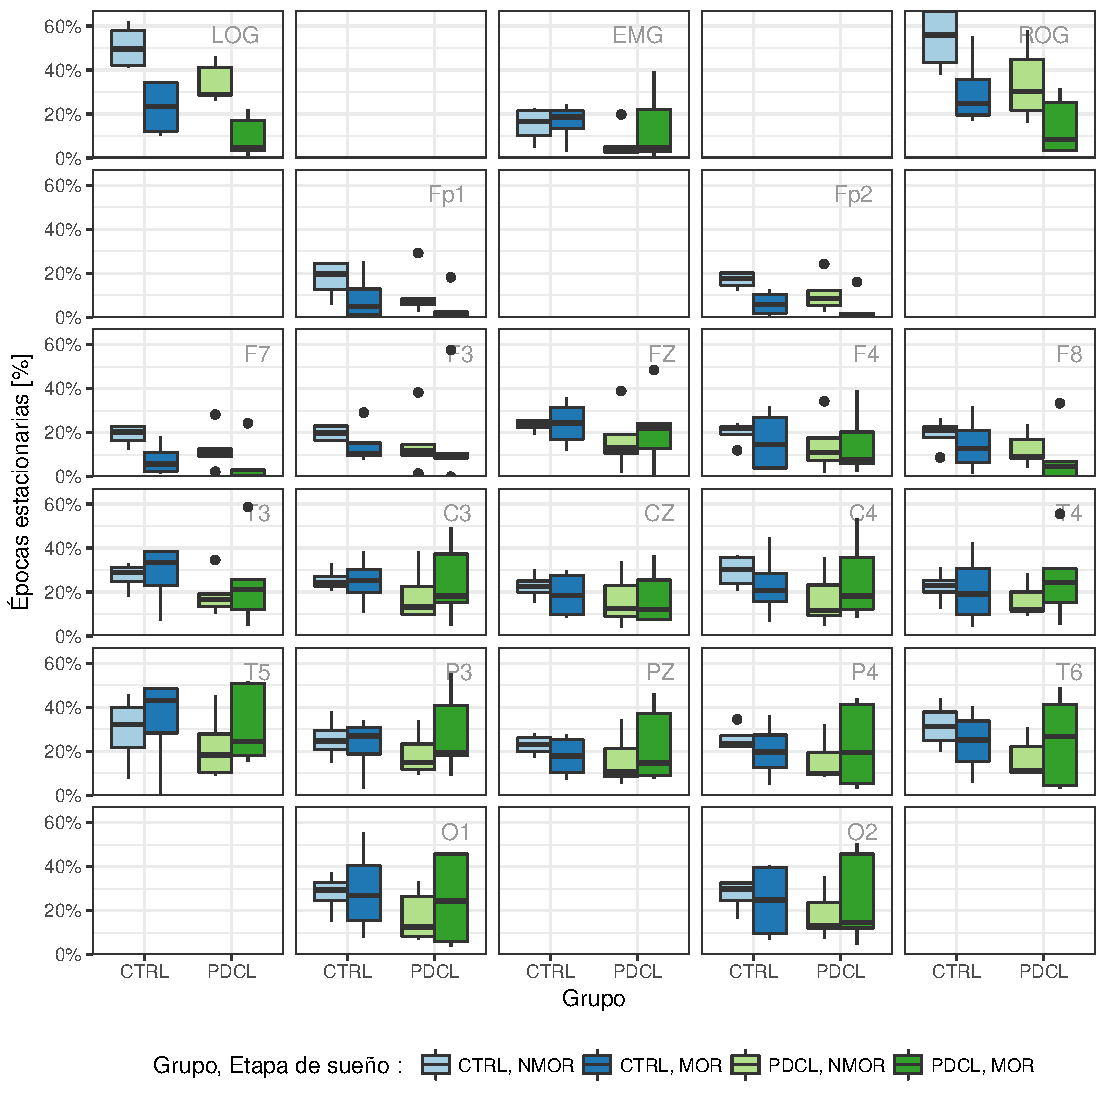
\includegraphics[width=\linewidth]
{./scripts_graf_res/comparacion_cabeza.pdf}
\caption{Proporciones de épocas estacionarias, durante sueño MOR y NMOR y para todas las derivaciones.
%
Los puntos representan valores \textit{atípicos}, según su definición para diagramas de caja.
%
Los asteriscos indican en qué derivaciones se hallaron \textit{efectos} significativos usando una ANOVA de dos factores: `etapa de sueño' y `grupo'; el efecto de `etapa de sueño' fue significativo para Fp2, F7, LOG y ROG, mientras que el efecto `grupo' fue significativo para LOG y ROG.
%
Las posiciones de cada gráfico se corresponden con aquellos de la figura \ref{img:estampa}.}
\label{comparacion_verde}
\end{figure}

%%%%%%%%%%%%%%%%%%%%%%%%%%%%%%%%%%%%%%%%%%%%%%%%%%%%%%%%%%%%%%%%%%%%%%%%%%%%%%%%%%%%%%%%%%%%%%%%%%%
%%%%%%%%%%%%%%%%%%%%%%%%%%%%%%%%%%%%%%%%%%%%%%%%%%%%%%%%%%%%%%%%%%%%%%%%%%%%%%%%%%%%%%%%%%%%%%%%%%%
%%%%%%%%%%%%%%%%%%%%%%%%%%%%%%%%%%%%%%%%%%%%%%%%%%%%%%%%%%%%%%%%%%%%%%%%%%%%%%%%%%%%%%%%%%%%%%%%%%%
%%%%%%%%%%%%%%%%%%%%%%%%%%%%%%%%%%%%%%%%%%%%%%%%%%%%%%%%%%%%%%%%%%%%%%%%%%%%%%%%%%%%%%%%%%%%%%%%%%%

\chapter{Discusión y Conclusiones}

Como se discutió en la sección \ref{sec:est_local}, se asume que el cerebro es un sistema complejo, cuya actividad se comporta como una secuencia organizada de fragmentos de actividad \textit{simple}.
%
Tal característica es referida como \textbf{estacionariedad local}, y la hipótesis descrita es que la actividad cerebral es localmente estacionaria.

En el presente trabajo la `hipótesis de estacionariedad local' fue manejada como un supuesto, y se hipotetizó que el DCL --o más en concreto, el PDCL-- \textit{afecta} la organización de la actividad cerebral respecto a la forma en que aparecen fragmentos de actividad simple.
%
De forma concreta, se decidió usar a la estacionariedad débil para declarar que los registros analizados son simples; de forma aún más concreta, se usó la prueba de estacionariedad débil de Priestley y Subba Rao para declarar si los registros analizados son débilmente estacionarios.

Conviene comentar que se eligió usar la estacionariedad débil porque es una cantidad \textit{sencilla}, que usualmente se asume pero no se verifica, y porque una gran cantidad de métodos de análisis la usan (esto será discutido más adelante).

Para facilitar la notación, se definieron las cantidades $\text{p}_{\text{MOR}}$ y $\text{p}_{\text{NMOR}}$, que representan la proporción de épocas durante las cuales los fragmentos de registro de PSG (sinónimo de épocas) \textit{son} débilmente estacionarios\footnote{Los registros de PSG son interpretados como observaciones de procesos estocásticos semi-estacionarios (ver definición \ref{def:semi_estacionario}); se dice que un fragmento de registro de PSG es débilmente estacionario si se puede rechazar la hipótesis de no--estacionariedad usando la prueba de Priestley--Subba Rao (ver sección \ref{sec:psr}).} durante MOR y NMOR, respectivamente; en otras palabras
\begin{equation}
\text{p}_{\text{MOR}} = \frac{\text{\# épocas estacionarias en MOR}}{\text{\# épocas en MOR}}
\end{equation}
y similarmente para $\text{p}_{\text{NMOR}}$. 
%
Estas cantidades son usadas debido a que la cantidad de épocas en MOR y NMOR son considerablemente diferentes, y así mismo son diferentes la cantidad de épocas en MOR y NMOR para los diferentes participantes.

Al probar la hipótesis $\text{p}_{\text{MOR}} \neq \text{p}_{\text{NMOR}}$ a nivel grupal (para lo cual se supuso que estas cantidades se distribuyen normalmente), se  encontró que hay diferencias significativas para las derivaciones Fp2, F7, LOG y ROG que pueden ser explicadas por el \textit{efecto} de la etapa se sueño, y de forma similar para las derivaciones LOG y ROG con el efecto de `grupo'.

Se describió una metodología con la cual, usando la clasificación de estacionariedad, se identificaron patrones de actividad que parecen \textit{responder} a las etapas de sueño.
%
Este enfoque no fue explorado más a fondo, pero proporciona evidencia \textit{a favor} de la hipótesis de estacionariedad local.

Las diferencias halladas en LOG y ROG pueden ser explicadas por las características del sueño MOR, ya que los movimientos oculares rápidos son una característica distintiva del sueño MOR --y que le dan nombre.

Por otro lado, las diferencias en Fp2 y F7 son \textit{prometedoras} porque el lóbulo frontal se asocia típicamente a funciones cognitivas; el nivel de significancia es débil, pero ello puede ser debido a que la muestra es relativamente pequeña.
%
Por ejemplo, en \cite{FRONTIERS} se usa un número ligeramente mayor de individuos junto otro método de análisis, obteniéndose resultados similares.

En necesario mencionar que hay una vasta cantidad de estudios que han explorado la posible relación entre trastornos del sueño y marcadores de daño neuronal o de actividad cerebral anómala \cite{porter15}.
%
De manera generalizada, dichos estudios han sido criticados por deficiencias metodológicas; entre ellos se encuentra el uso de grupos muestrales muy reducidos, de la auto-percepción por los pacientes como parámetro de medición, o incluso de pruebas neuropsicológicas con baja sensibilidad como el MMSE \cite{scullin15}.

Vale la pena mencionar que, como {contramedida} ante el efecto de grupos reducidos, se suele otorgar cierto \textit{prestigio} a las llamadas \textit{técnicas objetivas}, es decir, aquellas que son independientes del examinador.
%
La denominación de `técnicas objetivas' engloba, por ejemplo, a todos los registros electrofisiológicos y sus respectivos análisis cuantitativos (en contraparte a los análisis cualitativos); también es importante que se excluye la auto-percepción de deficiencias cognoscitivas, y las encuestas que no son suficientemente \textit{formales}.
%
Como consecuencia de lo anterior, se suele considerar que es posible extraer información fiable de grupos pequeños si se usan herramientas de análisis objetivas; como ejemplo está la revisión hecha por Yan Ma \cite{ma18}, donde predominan grupos relativamente pequeños.

Cabe destacar, como comentario, que la evidencia aportada \textit{apoya} a la hipótesis de estacionariedad local confirma el supuesto usual de que las señales de origen biológico son por naturaleza no-estacionarias; este resultado es importante para trabajos posteriores usando registros de PSG.

%%%%%%%%%%%%%%%%%%%%%%%%%%%%%%%%%%%%%%%%%%%%%%%%%%%%%%%%%%%%%%%%%%%%%%%%%%%%%%%%%%%%%%%%%%%%%%%%%%%
%%%%%%%%%%%%%%%%%%%%%%%%%%%%%%%%%%%%%%%%%%%%%%%%%%%%%%%%%%%%%%%%%%%%%%%%%%%%%%%%%%%%%%%%%%%%%%%%%%%

\section{Conclusiones}

%Es necesario mencionar que, de manera generalizada, muchos estudios han sido criticados por deficiencias metodológicas; entre ellos se encuentra el uso de grupos muestrales muy reducidos, de la auto-percepción por los pacientes como parámetro de medición, o incluso de pruebas neuropsicológicas con baja sensibilidad como el MMSE \cite{scullin15}.%

Se ha reportado que los cambios debidos al DCL están asociados con cambios en la estructura del sueño, y en particular en la etapa de sueño MOR.
%
Los resultados obtenidos indican que la clasificación de fragmentos de PSG como estacionarios responde a los cambios entre etapas de sueño, en particular al MOR y también entre los grupos.

Sin embargo, tampoco puede descartarse su utilidad para dicho fin, ya que muestra diferencias significativas para los patrones de actividad cerebral en la región frontal de la corteza cerebral, la cual se considera fisiológicamente relevante y tradicionalmente es asociada con la memoria y la toma de decisiones.

Respecto a la hipótesis de estacionariedad local (presentada en la sección \ref{sec:est_local}), la información recabada sugiere que dicha hipótesis se verifica para registros de PSG en adultos mayores.
%
Se hipotetiza que éste fenómeno explica los resultados {favorables} en dirección a la detección del PDCL \textit{usando}, y que un mejor entendimiento de dicho fenómeno podría usarse para optimizar la metodología descrita.

El hallazgo de patrones emergentes de estacionariedad (ver sección \ref{sec:analisis_registro}) sugiere que, en principio, es posible usar la clasificación de estacionariedad en registros de EEG para caracterizar estados de actividad cerebral. 
%
Esta posibilidad es interesante, pero va más allá de los objetivos del presente trabajo.

%%%%%%%%%%%%%%%%%%%%%%%%%%%%%%%%%%%%%%%%%%%%%%%%%%%%%%%%%%%%%%%%%%%%%%%%%%%%%%%%%%%%%%%%%%%%%%%%%%%
%%%%%%%%%%%%%%%%%%%%%%%%%%%%%%%%%%%%%%%%%%%%%%%%%%%%%%%%%%%%%%%%%%%%%%%%%%%%%%%%%%%%%%%%%%%%%%%%%%%

\section{Trabajo futuro}

Los resultados obtenidos son \textit{prometedores} y preliminares para declarar marcadores clínicos para el PDCL basados en la metodología descrita.
%
En el contexto de la colaboración con el Laboratorio de Sueño, Emoción y Cognición, la metodología será automatizada para poder analizar el total de registros obtenidos en el estudio por Vázquez Tagle y colaboradores.
%
Con base en los resultados obtenidos con un número mayor de participantes, se decidirá si se inicia un nuevo estudio para \textit{validar} la metodología descrita.

De manera general, el uso de marcadores basados en registros de PSG aporta una base objetiva al diagnóstico del deterioro cognitivo, y complementa los resultados más subjetivos de pruebas neuropsicológicas; esta afirmación permanece válida para una gran variedad de señales electrofisiológicas y trastornos mentales.
%
Conviene destacar que las técnicas basadas en el EEG son relativamente poco \textit{invasivas}, de bajo costo y fácil acceso, con relación a la calidad de la información obtenida y en comparación con otras técnicas para la observación del sistema nervioso central.
%
Entonces, generar marcadores diagnósticos tempranos basados en el EEG facilita su acceso para el público en general, en especial para detectar etapas tempranas del deterioro cognitivo.

En otro ámbito, los patrones emergentes de estacionariedad serán explorados en trabajos futuros.

%%%%%%%%%%%%%%%%%%%%%%%%%%%%%%%%%%%%%%%%%%%%%%%%%%%%%%%%%%%%%%%%%%%%%%%%%%%%%%%%%%%%%%%%%%%%%%%%%%%
%%%%%%%%%%%%%%%%%%%%%%%%%%%%%%%%%%%%%%%%%%%%%%%%%%%%%%%%%%%%%%%%%%%%%%%%%%%%%%%%%%%%%%%%%%%%%%%%%%%
%%%%%%%%%%%%%%%%%%%%%%%%%%%%%%%%%%%%%%%%%%%%%%%%%%%%%%%%%%%%%%%%%%%%%%%%%%%%%%%%%%%%%%%%%%%%%%%%%%%
%%%%%%%%%%%%%%%%%%%%%%%%%%%%%%%%%%%%%%%%%%%%%%%%%%%%%%%%%%%%%%%%%%%%%%%%%%%%%%%%%%%%%%%%%%%%%%%%%%%

\appendix

\chapter{Variables aleatorias}
\label{apendice:medidas}

En este apéndice se exponen algunos temas preliminares que, a fines del presente trabajo, se consideraron innecesarios.
%
Se incluye con el fin de clarificar algunos detalles sobre varios objetos usados durante el texto.
%
Se justifica la notación de \textit{derivadas generalizadas} que son usadas de forma común durante el texto.
%
Así mismo se definen las integrales respecto a procesos estocásticos, una parte fundamental de la representación espectral descrita en la sección \ref{sec:fde}, la cual a su vez es usada para demostrar varias propiedades del espectro evolutivo y sus estimadores.

%En suma, este apéndice puede ser omitido con el fin de usar la metodología descrita en el texto, pero es importante para entender la teoría \textit{detrás} de estas herramientas.

\section{Medidas}

\begin{definicion}%[$\boldsymbol{\sigma}$-álgebra]
Sea $\Omega$ un conjunto y sea $\mathcal{U}$ una familia de subconjuntos de $\Omega$. Se dice que $\mathcal{U}$ es una \textbf{$\boldsymbol{\sigma}$-álgebra} si cumple que
\begin{enumerate}[label=\MakeLowercase{\roman{*}})]
\item $\Omega \in \mathcal{U}$
\item $A \in \mathcal{U} \Rightarrow A^{C} \in \mathcal{U}$
\item $ \displaystyle \{ A_n \}_{n\in \mathbb{N}} \subseteq \mathcal{U} 
\Rightarrow \cup_{n\in \mathbb{N}} A_n \in \mathcal{U}$
\end{enumerate}
Donde $A^{C}$ es el complemento de $A$ en $U$. Los elementos de $\mathcal{U}$ se denominan \textbf{conjuntos medibles}. 
\end{definicion}

\begin{definicion}
Sea $\Omega$ un conjunto y $\mathcal{A} \subseteq \Omega$ una familia de subconjuntos. Se define a $\sigma(\mathcal{A})$, la \textbf{$\boldsymbol{\sigma}$-álgebra generada por $\boldsymbol{\mathcal{A}}$}, como la intersección de todas las $\sigma$-álgebras que contienen a $\mathcal{A}$.
\end{definicion}

\begin{ejemplo}
En el contexto de la probabilidad, es particularmente importante la \underline{$\sigma$-álgebra de Borel}, $\mathcal{B}$, definida como
\begin{equation}
\mathcal{B}_A := \sigma\left( \left\{ \left( -\infty , a \right] \subset \R \talque a\in \R \right\} \right)
\end{equation}
\end{ejemplo}

\begin{definicion}
Sea $\Omega$ un conjunto y $\mathcal{U}$ una $\sigma$-álgebra definida en $\Omega$. El par $(\Omega,\mathcal{U})$ será referido como \textbf{espacio de medida}. Por nomenclatura, $\Omega$ es referido como \textit{espacio muestral} y $\mathcal{U}$ como \textit{$\sigma$-álgebra de sucesos}.
\end{definicion}

\begin{definicion}%[Medida]
\label{medida}
Sea $(\Omega, \mathcal{U})$ un espacio de medida. Se dice que una función $\mu : \mathcal{U} \rightarrow \R_+$ es una \textbf{medida} si cumple que
\begin{itemize}
\item $\mu(\emptyset) = 0$
\item Si $\{ A_n \}_{n\in \mathbb{N}} \subseteq \mathcal{U}$ son tales que $A_n \cap A_m = \emptyset \Leftrightarrow m\neq n$, entonces 
\begin{equation}
\mu\left( \bigcup_{n\in \mathbb{N}} A_n \right) = \sum_{n\in \mathbb{N}} \mu(A_n)
\end{equation}
\end{itemize}
Donde $\R_+ = \left\{ x\in \R \talque 0 \leq x \right\} \cup \{ \infty \}$ y $\emptyset$ es el conjunto vacío. La terna $(\Omega,\mathcal{U},\mu)$ será referida como \textbf{espacio de medida}.
\end{definicion}

\begin{ejemplo}
Considérese el espacio medible $(\R, \mathcal{B})$, con $\mathcal{B}$ la $\sigma$-álgebra de Borel. Se define la \ul{medida de Lebesgue}, $\mu_L$, la medida en el espacio mencionado que satisface 
\begin{equation}
\mu_L\left(\left[a,b\right]\right) = b-a
\end{equation}
para cualesquiera $a,b \in \R$ con $a<b$. Por simplicidad, en lo posterior se dará por entendido que el espacio de medida $(\R, \mathcal{B},\mu_L)$ es \textit{usual} siempre que se hable de medidas en $\R$ o alguno de sus subconjuntos.
\end{ejemplo}

\begin{ejemplo}
Considérese el espacio medible $(\R, \mathcal{B})$, con $\mathcal{B}$ la $\sigma$-álgebra de Borel. Se define la \ul{medida discreta}, $\mu_D$, como
\begin{equation}
\mu_D(A) = \sum_{n \in A \cup \N} 1
\end{equation}
\end{ejemplo}

\begin{definicion}
Sea $(\Omega_1, \mathcal{U}_1)$ y $(\Omega_2, \mathcal{U}_2)$ dos espacios de medida. Se dice que una función $f:\Omega_1\rightarrow\Omega_2$ es una \textbf{función medible} si cumple que
\begin{equation}
U \in \mathcal{U}_2 \Rightarrow f^{-1}(U) \in \mathcal{U}_1 
\end{equation}
donde $f^{-1}(U) = \left\{ u\in \Omega_1 \talque f(u) \in U \right\}$.
\end{definicion}

%%%%%%%%%%%%%%%%%%%%%%%%%%%%%%%%%%%%%%%%%%%%%%%%%%%%%%%%%%%%%%%%%%%%%%%%%%%%%%%%%%%%%%%%%%%%%%%%%%%
%%%%%%%%%%%%%%%%%%%%%%%%%%%%%%%%%%%%%%%%%%%%%%%%%%%%%%%%%%%%%%%%%%%%%%%%%%%%%%%%%%%%%%%%%%%%%%%%%%%

\section{Variables aleatorias}

Si una medida $\mu$ es acotada en todo el espacio de eventos se dice que es una \textbf{medida finita}.
%
Una medida de probabilidad puede entenderse como un caso particular de medida finita sobre $\R$.

\begin{definicion}
El espacio de medida $(\Omega,\mathcal{U},P)$ se dice un \textbf{espacio de probabilidad} si satisface que $P(\Omega) = 1$.
\end{definicion}

\begin{definicion}
\label{lazy4}
Sea $(\Omega,\mathcal{U})$ un espacio medible y $(I,\mathcal{B}_I,P)$ un espacio de probabilidad. Una \textbf{variable aleatoria} es una función medible $X: \Omega \rightarrow \mathcal{B}_I$.
\end{definicion}

\begin{definicion}
Una \textbf{variable aleatoria real} es un caso particular de variable aleatoria entre el espacio de medida $(\R,\mathcal{B},\mu_L)$ consigo mismo.
\end{definicion}

\begin{definicion}%[Función de Probabilidad Acumulada]
Sea $X$ una variable aleatoria real. Su \textbf{función de probabilidad acumulada}, $F_X : \R \rightarrow [0,1]$, se define como
\begin{equation*}
F_X (x) := P\left( \left(-\infty,x \right] \right)
\end{equation*}
\end{definicion}

\begin{proposicion}
Sea $X$ una variable aleatoria real y $F$ su función de probabilidad acumulada. $F$ satisface las siguientes propiedades:
\begin{itemize}
\item Para cualesquiera $x,y\in \R$, $x < y \Rightarrow F(x) < F(y)$
\item Para cualquier $x\in\R$, $F(x) = \left[\lim_{y\rightarrow x^{-}} F(y)\right] + P\left(\left\{x\right\}\right)$
\item $\lim_{x\rightarrow +\infty} F(x) = 1$
\item $\lim_{x\rightarrow -\infty} F(x) = 0$
\end{itemize}
\end{proposicion}

\begin{definicion}
Sea $X$ una variable aleatoria real y $F$ su función de probabilidad acumulada. Si existe una función $f$  tal que puede escribirse
\begin{equation}
P(x\in A) = \int_A f_X(\lambda) d\lambda 
\end{equation}
entonces se dice que $f$ es la \textbf{función de densidad de probabilidad} de $X$.
\end{definicion}

Conviene destacar a las funciones que satisfacen las propiedades de una función de distribución pero que no necesariamente están asociadas a ninguna variable aleatoria real.
%
Este tipo de funciones, referidas como \textbf{funciones de distribución}, merecen especial atención porque pueden inducir variables aleatorias.

\begin{proposicion}
Sea $F:\R \rightarrow \R$ una función de distribución; se puede construir una medida $\mu_F$ sobre el espacio medible $(\R, \mathcal{B})$ tal que la función de probabilidad acumulada asociada al espacio de probabilidad $(\R, \mathcal{B}, \mu_F)$ es exactamente $F$.
%
La medida $\mu_F$ será referida como la \textbf{medida inducida} por $F$.
\end{proposicion}

Así entonces, es perfectamente posible definir variables aleatorias especificando su respectiva función de probabilidad acumulada, o su función de densidad de probabilidad cuando ello sea posible.
%
Para dicho fin conviene introducir la notación $X \sim Y$ para dos variables aleatorias que tienen la misma función de probabilidad acumulada.

\begin{ejemplo}
Se dice que una variable aleatoria real $X$ es \ul{degenerada} en $z\in \R$, lo cual se denota por $X\sim D(z)$, si su función de probabilidad acumulada es de la forma
\begin{equation}
F(x) = \begin{cases}
0 &, x < 0 \\
1 &, z \leq x
\end{cases}
\end{equation}
\end{ejemplo}

\begin{ejemplo}
Se dice que una variable aleatoria real $X$ sigue una \ul{distribuci\'on uniforme} con parámetros $a, b \in \R$, lo cual se denota por $X\sim \text{unif}(a,b)$ si su función de densidad de probabilidad es de la forma
\begin{equation}
f(x) = 
\begin{cases}
\frac{1}{b-a} &, a\leq x \leq b \\
0 &, \text{otro caso}
\end{cases}
\end{equation}
\end{ejemplo}

\begin{ejemplo}
Se dice que una variable aleatoria real $X$ sigue una \ul{distribuci\'on normal} con parámetros $\mu, \sigma \in \R$, lo cual se denota por $X\sim \text{N}(\mu,\sigma^{2})$ si su función de probabilidad acumulada es de la forma
\begin{equation}
F(x) = \frac{1}{\sqrt{2 \pi \sigma^{2}}} \int_{-\infty}^{x} e^{-\frac{(x-\mu)^{2}}{2}} dx
\end{equation}
\end{ejemplo}

\begin{ejemplo}
Se dice que una variable aleatoria real $X$ sigue una \ul{distribuci\'on $\chi^2$} con parámetro $\nu\in \R_+$, lo cual se denota por $X\sim \chi^2(\nu)$, si su función de distribución de probabilidad es de la forma
\begin{equation}
f(x) = \begin{cases}
\left[ 2^{\nicefrac{\nu}{2}} \Gamma(\nicefrac{\nu}{2}) \right]^{-1} x^{\nicefrac{\nu}{2}-1} e^{-\nicefrac{x}{2}} &, 0 < x \\
0 &, \text{otro caso}
\end{cases}
\end{equation}
donde $\Gamma: \R_+ \rightarrow \R$ es la \underline{función gamma}, definida como
\begin{equation}
\Gamma(x) := \int_{0}^{\infty} t^{x-1} e^{-t} dt
\end{equation}
\end{ejemplo}

\begin{ejemplo}
Se dice que una variable aleatoria real $X$ sigue una \ul{distribuci\'on F de Fisher} con parámetros $m, n \in \N$, lo cual se denota por $X\sim \text{F}(m,n)$, si su función de densidad de probabilidad es de la forma
\begin{equation}
f(x) = \frac{1}{B(\nicefrac{m}{2},\nicefrac{n}{2})} \left[ \frac{m x}{m x + n} \right]^{\nicefrac{m}{2}} \left[ 1- \frac{m x}{m x + n} \right]^{\nicefrac{n}{2}} x^{-1}
\end{equation}
donde $B: \R_+^2 \rightarrow \R$ es la \underline{función beta}, definida como
\begin{equation}
B(m,n) := 2 \int_0^{\nicefrac{\pi}{2}} \left[\COS{\theta} \right]^{2x-1} \left[\SEN{\theta} \right]^{2y-1} d\theta
\end{equation}
\end{ejemplo}

%%%%%%%%%%%%%%%%%%%%%%%%%%%%%%%%%%%%%%%%%%%%%%%%%%%%%%%%%%%%%%%%%%%%%%%%%%%%%%%%%%%%%%%%%%%%%%%%%%%
%%%%%%%%%%%%%%%%%%%%%%%%%%%%%%%%%%%%%%%%%%%%%%%%%%%%%%%%%%%%%%%%%%%%%%%%%%%%%%%%%%%%%%%%%%%%%%%%%%%

\subsection{Valor esperado}

\begin{definicion}
Sea $X$ una variable aleatoria real y sea $P$ su medida asociada. Se define el \textbf{valor esperado} de $X$ como
\begin{equation}
\E{X} := \int_\Omega X(\lambda) dP(\lambda)
\end{equation}
\end{definicion}

\begin{proposicion}
Sea $X$ una variable aleatoria real, y sea $g$ una función medible en el espacio medible $(\R,\mathcal{B},P_X)$. Entonces $g(X)$ es una variable aleatoria cuyo valor esperado es
\begin{equation}
\E{g(x)} = \int_\Omega [g(X)](\lambda) dP(\lambda) = \int_\R g(x) dP(x)
\end{equation}
\end{proposicion}

\begin{definicion}
Sea $X$ una variable aleatoria real. Si las siguientes cantidades están bien definidas
\begin{align}
\mu_X &{:=} \E{X} \\
\sigma_X^{2} &{:=} \E{(X-\mu_X)^{2}}
\end{align}
entonces se dice que $\mu_X$ es la \textbf{media}\footnote{La notación $\mu_X$ únicamente es usada cuando no hay confusión con la notación para medidas.} de $X$, y $\sigma^2$ es su \textbf{varianza}.
%Por definición, no hay garantía que una variable aleatoria arbitraria tenga media o varianza bien definidas.
\end{definicion}

%%%%%%%%%%%%%%%%%%%%%%%%%%%%%%%%%%%%%%%%%%%%%%%%%%%%%%%%%%%%%%%%%%%%%%%%%%%%%%%%%%%%%%%%%%%%%%%%%%%
%%%%%%%%%%%%%%%%%%%%%%%%%%%%%%%%%%%%%%%%%%%%%%%%%%%%%%%%%%%%%%%%%%%%%%%%%%%%%%%%%%%%%%%%%%%%%%%%%%%

\subsection{Vectores aleatorios}

El concepto de variable aleatoria real es sólo un caso particular de variable aleatoria (definición \ref{lazy4}), el cual puede puede usarse para otros conjuntos de interés.
%
A continuación se presenta el caso de $\R^{n}$ para algún $n\in \N$.

\begin{definicion}
Se llama \textbf{vector aleatorio} a una variable aleatoria sobre el espacio de probabilidad $(\R^{n},\mathcal{B}^{n},P)$, para algún $n\in \N$. Se define a $\mathcal{B}^{n}$, la $\sigma$-álgebra de Borel $n$-dimensional, como
\begin{equation}
\mathcal{B}^{n} := \sigma\left(\left\{ \left(-\infty, a_1\right]\times \left(-\infty, a_2\right]\times \cdots \times \left(-\infty, a_n\right] \lvert a_1, \dots, a_n \in \R \right\}\right)
\end{equation}
\end{definicion}

Por notación, el vector aleatorio \textit{$n$-dimensional} $\boldsymbol{X}$ será referido como
\begin{equation}
\boldsymbol{X} = [X_1, X_2, \dots, X_n]
\end{equation}
esta notación de vectores con \textit{símbolos gruesos} será usada durante el texto, extendida igualmente para realizaciones y otros vectores similares.

\begin{definicion}
Sean $X$, $Y$ dos variables aleatorias, cuyas medidas asociadas son $P_X$ y $P_Y$, y sea $P_{[X,Y]}$ la medida asociada al vector $[X,Y]$. Se define la \textbf{covarianza} entre $X$ y $Y$ como
\begin{equation}
\Cov{X,Y} := \E{X Y} = \int_{\R^{2}} x y\, d P_{[X,Y]}(x,y)
\end{equation}
\end{definicion}

\subsection{Integración y procesos estocásticos}
\label{sec:int_proc_est}

El proceso de integración puede extenderse intuitivamente respecto a procesos estocásticos.
%
%Este tema no será explorado con mayor detalle en el presente texto, sino que sólo será usado para construir algunos ejemplos.
%
Para ello se define al proceso de Wiener, un proceso estocástico con algunas propiedades peculiares que serán de gran utilidad.

\begin{ejemplo}
Un \underline{proceso de Wiener} es un proceso estocástico $\{ W(t)\}_{t\in\R}$ que satisface las siguientes propiedades para cualesquiera $t, s, \in \R$
\begin{itemize}
\item $W(0) \sim \text{D}(0)$
\item $\left[W(t)-W(s)\right] \sim N(0, \abso{t-s})$
\item $\left[W(t)-W(s)\right]$ es independiente de $W(u)$ para $u < \min\{ t, s \}$
\end{itemize}

Es relativamente fácil notar que $\E{W(t)} = 0$ y $\E{\left(W(t)\right)^2}$, de donde se deduce que el proceso de Wiener no es débilmente estacionario.
\end{ejemplo}

Así entonces, sea $\{ W(t)\}_{t\in\R}$ un proceso de Wiener, $[a,b]\subseteq\R$ un intervalo arbitrario, y $f:[a,b]\longrightarrow\R_+$ una función medible.
%
Sean $t_1, t_2, \dots, t_N \in \R$ una partición arbitraria de $[a,b]$, es decir que satisfacen
\begin{equation}
a < t_1 < t_2 < \dots < t_N < b
\end{equation}
entonces se define la variable aleatoria
\begin{equation}
\sum_{i=2}^N \left[ \sup_{\lambda \in [t_{i-1},t_i]} f(\lambda) \right] \left[ W(t_i) - W(t_{i-1}] \right)
\end{equation}

\underline{Si} la colección de variables aleatorias converge en media cuadrática entonces se dice que
\begin{equation}
\int_a^b f(t) dW(t) :=
\lim_{N\rightarrow \infty} \left(
\sum_{i=2}^N \left[ \sup_{\lambda \in [t_{i-1},t_i]} f(\lambda) \right] \left[ W(t_i) - W(t_{i-1}] \right] \right)
\end{equation}

\begin{proposicion}
\label{prop:lazy000}
Sea $\{ W(t)\}_{t\in\R}$ un proceso de Wiener, $[a,b]\subseteq\R$ un intervalo arbitrario, y $f:[a,b]\longrightarrow\R_+$ una función medible. Entonces
\begin{equation}
\E{\int_a^b f(t) dW(t) } = 0
\end{equation}
\end{proposicion}
\begin{proof}
Sea $\Delta W_i = W(t_i) - W(t_{i-1})$, el cual satisface las siguientes propiedades
\begin{itemize}
\item $\E{\Delta W_i} = 0$
\item $\E{\left( \Delta W_i \right)^2} = t_{i} - t_{i-1}$
\item Si $i<j$ entonces $\Delta W_i$ y $\Delta W_j$ son independientes
\end{itemize} 

Entonces, nótese que
\begin{align*}
\E{\int_a^b f(t) dW(t) } &=
\E{ \lim_{N\rightarrow \infty} \left( \sum_{i=2}^N f_i \Delta W_i \right) } \\
&= 
\lim_{N\rightarrow \infty} \left( \sum_{i=2}^N f_i \E{ \Delta W_i } \right) \\
&= 0
\end{align*}
donde $f_i = \sup_{\lambda \in [t_{i-1},t_i]} f(\lambda)$.
\end{proof}

\begin{proposicion}
\label{prop:lazy100}
Sea $\{ W(t)\}_{t\in\R}$ un proceso de Wiener, $[a,b]\subseteq\R$ un intervalo arbitrario, y $f:[a,b]\longrightarrow\R_+$ una función medible. Entonces
\begin{equation}
\E{\left(\int_a^b f(t) dW(t) \right)^2 } = \int_a^b \left[ f(t) \right]^2 dt
\end{equation}
\end{proposicion}
\begin{proof}
Sea $\Delta W_i = W(t_i) - W(t_{i-1})$, como en la demostración anterior.
Nótese que
\begin{align*}
\E{\left(\int_a^b f(t) dW(t) \right)^2 } &=
\E{\left( \lim_{N\rightarrow \infty} \left(
\sum_{i=2}^N f_i \Delta W_i \right) \right)^2} \\
&= 
\lim_{N\rightarrow \infty} \E{ \left(
\sum_{i=2}^N f_i \Delta W_i \right)^2} \\
&=
\lim_{N\rightarrow \infty} \sum_{i=2}^N \sum_{j=2}^N
f_i f_j \E{  \Delta W_i \Delta W_j } \\
&=
\lim_{N\rightarrow \infty} \sum_{i=2}^N
f_i^2 \E{  \left( \Delta W_i \right)^2 } \\
&=
\lim_{N\rightarrow \infty} \sum_{i=2}^N
f_i^2 (t_i-t_{i-1}) \\
&=
\int_a^b \left[ f(t) \right]^2 dt
\end{align*}
donde $f_i = \sup_{\lambda \in [t_{i-1},t_i]} f(\lambda)$.
\end{proof}

\begin{ejemplo}
Sea $\{ W(t)\}_{t\in\R}$ un proceso de Wiener y sea $A\in\R_+$ arbitrario. Se define a $\{Y(t)\}_{t\in\R}$, un \underline{proceso medias m\'oviles tiempo continuo} con parámetro $A$, como
\begin{equation}
Y(t) = \frac{1}{A}\int_{t-\nicefrac{A}{2}}^{t+\nicefrac{A}{2}} dW(u)
\end{equation}

Con base a la proposición \ref{prop:lazy000}, se deduce que
\begin{equation}
\E{Y(t)} = 0
\end{equation}
Así mismo, usando la proposición \ref{prop:lazy100} se deduce la función de autocovarianza
\begin{align*}
\E{Y(t)Y(s)} &= 
\E{ \left( \frac{1}{A}\int_{\Omega_t} dW(u) \right) \left( \frac{1}{A}\int_{\Omega_s} dW(v)\right) } \\
&= 
\frac{1}{A^2} 
\E{ 
\left( 
\int_{\Omega_t \cap \Omega_s^C} dW(u) + \int_{\Omega_t \cap \Omega_s} dW(u) 
\right)
\left( 
\int_{\Omega_s \cap \Omega_t^C} dW(v) + \int_{\Omega_t \cap \Omega_s} dW(v) 
\right)  
} \\
&=
\frac{1}{A^2} 
\E{  
\int_{\Omega_t \cap \Omega_s^C} dW(u)  
}
\E{
\int_{\Omega_s \cap \Omega_t^C} dW(v) 
} \\
&\pheq
+ \frac{1}{A^2} 
\E{ 
\int_{\Omega_t \cap \Omega_s^C} dW(u)  
}
\E{
 \int_{\Omega_t \cap \Omega_s} dW(v) 
} \\
&\pheq
+\frac{1}{A^2} 
\E{ 
\int_{\Omega_t \cap \Omega_s} dW(u) 
}
\E{
\int_{\Omega_s \cap \Omega_t^C} dW(v)
} \\
&\pheq
+\frac{1}{A^2} 
\E{ 
\left( 
\int_{\Omega_t \cap \Omega_s} dW(u) 
\right)^2
} \\
&= \frac{1}{A^2} \max \{ A-\abso{t-s}, 0 \}
\end{align*}
donde $\Omega_t = \left[ t - \nicefrac{A}{2}, t + \nicefrac{A}{2} \right]$ y similarmente para $\Omega_s$.
%
En particular, el proceso de medias móviles a tiempo continuo es débilmente estacionario.
%
Por simplicidad, este proceso será referido simplemente como \textit{proceso medias móviles}.
\end{ejemplo}

%%%%%%%%%%%%%%%%%%%%%%%%%%%%%%%%%%%%%%%%%%%%%%%%%%%%%%%%%%%%%%%%%%%%%%%%%%%%%%%%%%%%%%%%%%%%%%%%%%%
%%%%%%%%%%%%%%%%%%%%%%%%%%%%%%%%%%%%%%%%%%%%%%%%%%%%%%%%%%%%%%%%%%%%%%%%%%%%%%%%%%%%%%%%%%%%%%%%%%%
%%%%%%%%%%%%%%%%%%%%%%%%%%%%%%%%%%%%%%%%%%%%%%%%%%%%%%%%%%%%%%%%%%%%%%%%%%%%%%%%%%%%%%%%%%%%%%%%%%%
%%%%%%%%%%%%%%%%%%%%%%%%%%%%%%%%%%%%%%%%%%%%%%%%%%%%%%%%%%%%%%%%%%%%%%%%%%%%%%%%%%%%%%%%%%%%%%%%%%%

\chapter{Propiedades formales del espectro de potencias}
\label{apendice:espectral}

%Este apéndice se presenta con el fin de lograr un texto autocontenido; bajo esta línea de pensamiento, este apéndice es un soporte para el capítulo \ref{capitulo:espectro_evo}, conteniendo las demostraciones formales de algunas propiedades 
Este apéndice representa una \textit{extensión} del capítulo \ref{capitulo:espectro_evo}; 
%contempla varias propiedades importantes del espectro evolutivo y sus estimadores, pero que no se consideraron como indispensable en el contexto del trabajo.
%
bajo esta línea de pensamiento puede decirse que el objetivo de este apéndice es demostrar las propiedades usadas en el trabajo, y exhibir algunos objetos \textit{conocidos}.
% objetos que no se consideraron relevantes pese a que son efectivamente importantes.

\section{Espacios de variables aleatorias}
\label{sec:espacios_aleatorios}

Tanto el espectro de potencias como el espectro evolutivo (siendo el segundo una generalización del primero) son generalizaciones de la transformada de Fourier;
%
%La mejor forma de entender la transformada de Fourier es como una función lineal entre espacios de Hilbert, de modo 
%
para definir a la transformada de Fourier se requiere, cuando menos, estructura de espacio de Hilbert.
%
En el contexto de procesos estocásticos, es recomendable la exposición sobre espacios de Hilbert en el libro \textit{``Stationary Stochastic Processes: Theory and Applications"} por Georg Lindgren \cite{estacionariedad_lindgren}.

\begin{proposicion}
\label{teo:hilbert_random}
Sea $\mathcal{A}$ el conjunto de variables aleatorias con media cero y varianza finita. Se define un producto interno entre dos variables aleatorias arbitrarias, $U$ y $V$, como
\begin{equation}
\langle U , V \rangle := \E{U, \overline{V}}
\end{equation}
Usando la suma y productos usuales de variables aleatorias, junto al producto interno descrito, el espacio $\mathcal{A}$ tiene la estructura de espacio de Hilbert.
\end{proposicion}

Basta con notar algunas propiedades de las variables aleatorias:
\begin{itemize}
\item Es posible sumar variables aleatorias, aún si la variable resultante tiene una distribución degenerada. El neutro aditivo es la variable con distribución degenerada $D(0)$.
\item Si todas las variables tienen media cero, la covarianza es una función bilineal, es decir que para cualesquiera $X,Y,Z \in \mathcal{A}$ y cualesquiera $a\in \R$
\begin{equation}
\Cov{aX+Y,Z} = a\Cov{X,Z} + \Cov{Y,Z}
\end{equation}
\end{itemize}

Merece especial atención la métrica inducida en el espacio de las variables aleatorias de media cero y varianza finita, $\mathcal{A}$, ya que implica un criterio de convergencia para variables aleatorias.
%; el criterio de convergencia para variables aleatorias, según dicha métrica, es precisamente la convergencia en media cuadrática.

\begin{definicion}%[Continuidad estocástica en media cuadrática]
\label{cont_est}
Un proceso a tiempo continuo \xt se dice \textbf{estocásticamente continuo en media cuadrática}, en el tiempo $t_0\in \mathcal{T}$ si
\begin{equation}
\lim_{t \rightarrow t_0} \E{\left( X(t) - X(t_0) \right)^{2}} = 0
\end{equation}
\end{definicion}

Es también muy interesante notar que los procesos estocásticos pueden interpretarse como \textit{curvas} en $\mathcal{A}$ indexadas por el tiempo.
%
La condición de continuidad estocástica se traduce en que tales curvas sean continuas.

\begin{proposicion}
Sea \xt un proceso estocástico a tiempo continuo y $R$ su núcleo de covarianza.
%
Si $R$ es continuo en el conjunto $\left\{ (t,t) \in \R^2 \talque t\in \R \right\}$ entonces \xt es estocásticamente continuo en $\mathcal{T}$.
\end{proposicion}

\begin{proof}
Sea $t_0\in\mathcal{T}$ arbitrario. Para cualquier $t\in \mathcal{T}$, puede escribirse
\begin{align*}
\E{\left( X(t) - X(t_0) \right)^{2}} &= \Var{X(t)} + \Var{X(t_0)} - 2 \Cov{X(t),X(t_0)} \\
&= R(t,t) + R(t_0,t_0)  - 2 R(t,t_0) \\
&= \left[ R(t,t) - R(t,t_0) \right] + \left[ R(t_0,t_0)  - R(t,t_0) \right]
\end{align*}
Así entonces, la condición para continuidad estocástica puede reescribirse como
\begin{align*}
\lim_{t \rightarrow t_0} \E{\left( X(t) - X(t_0) \right)^{2}} = 0 
&\Leftrightarrow
\lim_{t \rightarrow t_0} \left( \left[ R(t,t) - R(t,t_0) \right] + \left[ R(t_0,t_0)  - R(t,t_0) \right] \right) = 0 \\
&\Leftarrow 
\lim_{t \rightarrow t_0} \left[ R(t,t) - R(t,t_0) \right] = 0 \quad , \quad \lim_{t \rightarrow t_0} \left[ R(t_0,t_0)  - R(t,t_0) \right] = 0 
\end{align*}
Las últimas condiciones se siguen de que $R$ es continua en $\left\{ (t,t) \in \R^2 \talque t\in \R \right\}$.
\end{proof}

\begin{figure}
\centering
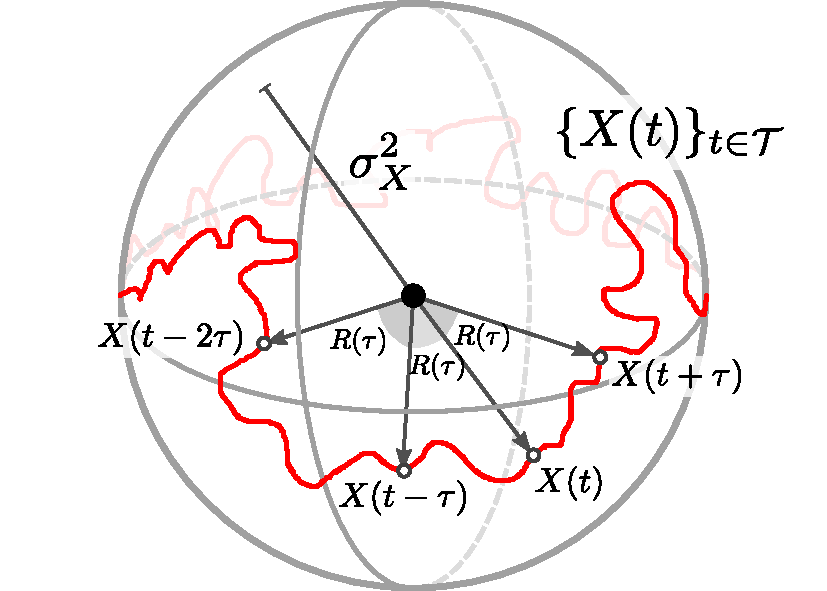
\includegraphics[width=.6\textwidth]{./img_diagramas/esfera_v1.pdf}
\caption[Geometría esperada para un proceso estocástico débilmente estacionario y estocásticamente continuo \textit{dentro} del espacio de variables aleatorias con varianza finita.]{Geometría esperada para un proceso estocástico débilmente estacionario y estocásticamente continuo, \xt , \textit{dentro} del conjunto de variables aleatorias con varianza finita, $\mathcal{A}$.
%
El objetivo de esta ilustración es visualizar algunos \textit{elementos} de \xt dentro del contexto de $\mathcal{A}$ como un espacio de Hilbert. Por ejemplo \xt está contenido en una esfera de radio $\sigma_X^2$ y centro en una variable aleatoria con distribución degenerada $D(0)$.}
\end{figure}

De igual forma es muy notable la interpretación que adquiere la función de autocovarianza como producto interno, ya que admite algunas propiedades interesantes.
%, tomando en cuenta que la covarianza es el producto interno del espacio; ya antes se demostró que la función de autocovarianza es una función definida positiva (proposición \ref{lazy:meh}), así que es posible inducirle una representación al estilo de la transformada de Fourier usando el siguiente teorema.

\begin{definicion}
Se dice que una función $f: \R\rightarrow \R$ es \textbf{positiva definida} si para cualesquiera $x_1, _2, \cdots, x_N \in \R$, $z_1, z_2, \cdots, z_N \in \R$ se cumple que 
\begin{equation}
\sum_{n=1}^{N} \sum_{m=1}^{N} z_n z_m f(x_m-x_n) \leq 0
\end{equation}
\end{definicion}
\newpage

\begin{proposicion}
\label{lazy:meh}
Sea \xt un proceso débilmente estacionario y $R^\star$ su función de autocovarianza. Se cumple que $R$ es una función positiva definida.
\end{proposicion}

\begin{proof}
Sean $t_1, t_2, \cdots, t_N \in \mathcal{T}$, $z_1, z_2, \cdots, z_N \in \R$ arbitrarios. Se construye la variable aleatoria $W$ como
\begin{equation}
W = \sum_{n=1}^{N} z_n X(t_n)
\end{equation}

Ahora, nótese que
\begin{align*}
0 &\leq \Var{W} \\
&= \sum_{m=1}^{N} \sum_{n=1}^{N} z_m z_n \Cov{X(t_m),X(t_n)} \\
&= \sum_{m=1}^{N} \sum_{n=1}^{N} z_m z_n R^\star(t_m-t_n)
\end{align*}
\end{proof}

\begin{teorema}[Bochner]
Sea $f:\R\rightarrow \R$ una función real arbitraria. Una condición suficiente y necesaria para que $f$ sea definida positiva es que exista una función $F:\R\rightarrow \R$ monótonamente creciente, continua por la derecha y acotada tal que
\begin{equation}
f(t) = \intR e^{i \omega t} dF(\omega)
\end{equation}
\end{teorema}

Del teorema de Bochner, aplicado a la función de autocovarianza, se sigue la existencia de los espectro de potencias para procesos estocásticos débilmente estacionarios (ver teorema \ref{t_wienerkhinchin}).
%
Dado que los núcleo de covarianza no son, en general, funciones positivas definidas, la existencia del espectro de potencias no está garantizada para cualquier proceso estocástico arbitrario.
%
Conviene notar que una condición similar se exige para la existencia del espectro evolutivo, cuando se pide que el núcleo de covarianza tenga un representación de la forma
\begin{equation}
R(s,t) = \intR \overline{\phi(\omega;s)}\phi(\omega;t) d\mu(\omega)
\end{equation}

%La estructura del espacio $\mathcal{A}$ no será explorada de forma más profunda en el presente trabajo, sino que sólo es usada para exponer el contexto del teorema de Bochner; este último será usado para definir al espectro de potencias.

%%%%%%%%%%%%%%%%%%%%%%%%%%%%%%%%%%%%%%%%%%%%%%%%%%%%%%%%%%%%%%%%%%%%%%%%%%%%%%%%%%%%%%%%%%%%%%%%%%%
%%%%%%%%%%%%%%%%%%%%%%%%%%%%%%%%%%%%%%%%%%%%%%%%%%%%%%%%%%%%%%%%%%%%%%%%%%%%%%%%%%%%%%%%%%%%%%%%%%%

\section{Espectro de potencias y representación espectral}
\label{sec:fde}

%Una vez definido el espacio $\mathcal{A}$, la existencia del espectro de potencias para procesos débilmente estacionarios está dado por el siguiente teorema.

\begin{teorema}[Wiener-Khintchine]
\label{t_wienerkhinchin}
Una condición suficiente y necesaria para que $R$ sea una función de autocovarianza para algún proceso estocástico a tiempo continuo \xt débilmente estacionario y estocásticamente continuo, es que exista una función $H: \R\rightarrow\R$ monótonamente creciente y acotada\footnote{Para lograr la unicidad, se pedirá que $\lim_{\omega\rightarrow -\infty} H(\omega) = 0$.} tal que para todo $\tau \in \R$ se cumple que
\begin{equation*}
R(\tau) = \intR e^{i \omega \tau} dH(\omega)
\end{equation*}
Como notación, $H$ será referido como la \textbf{función de espectro integrado} para \xt.
%
Adicionalmente, si $H$ es absolutamente continua, se define a $h$, la \textbf{función de densidad espectral} como
\begin{equation}
h(\omega) d\omega := dH(\omega)
\end{equation}
\end{teorema}


\begin{proposicion}
\label{rep_espectral}
Sea \xt un proceso estocástico a tiempo continuo, estocásticamente continuo, y sea $R$ su núcleo de covarianza.
%
Si $R$ admite una representación de la forma
\begin{equation}
R(s,t) = \intR \overline{\phi(\omega;s)}\phi(\omega;t) d\mu(\omega)
\end{equation}
entonces \xt acepta una representación de la forma
\begin{equation}
X(t) = \intR \phi(\omega; t) dZ(\omega)
\end{equation}
donde $\{ Z(t) \}_{t\in \R}$ es un proceso estocástico tal que
\begin{equation}
\Cov{Z(t),Z(s)} = \delta(t,z) \mu(\omega)
\end{equation}
con $\delta$ la función delta de Kronecker.
\end{proposicion}

\newpage
\begin{proof}
Considerando a $\mathcal{A}$, el espacio de variables aleatorias descrito en la proposición \ref{teo:hilbert_random}. 
%
Usando el producto interno descrito, para cualesquiera $t,s\in\R$ puede escribirse
\begin{equation}
\pint{X(t),X(s)} = \Cov{X(t),X(s)} = \intR \phi(\omega; t) \overline{\phi(\omega; s)} d\mu(\omega)
\end{equation} 

Usando la familia de funciones $\{ \phi(\bullet; t) \}_{t\in \mathcal{T}}$ y la medida $\mu$, puede construirse un segundo espacio de Hilbert, $\mathcal{H}_\phi$.
%
A este segundo espacio se le define el producto interno
\begin{equation}
\pint{\phi_1,\phi_2}_H := \intR \phi_1(\omega) \overline{\phi_2(\omega)} dH(\omega)
\end{equation} 

Posteriormente se define un mapeo $M : \mathcal{H}_\phi \rightarrow \mathcal{R}$ como
\begin{equation}
M[\phi_t] := X(t)
\end{equation}
el cual se extiende linealmente para cualesquiera coeficientes $c_1, c_2, \cdots \in \R$ y tiempos admisibles $t_1, t_2, \cdots \in \mathcal{T}$
\begin{equation}
M\left[ \sum_i c_i \phi_{t_i} \right] = \sum_i c_i M\left[ \phi_{t_i} \right]
\end{equation}

Trivialmente, $M$ conserva productos internos; basta notar que
\begin{equation}
\pint{X(t),X(s)} = \intR \phi_1(\omega) \overline{\phi_2(\omega)} dH(\omega) = \pint{\phi_1,\phi_2}_H
\end{equation}

Ahora, para trabajar con las funciones $\phi$ conviene descomponerlas en una base más \textit{sencilla}, como límite de funciones simples. Para ello, se define una función indicadora
\begin{equation}
I(\omega; \omega_0, \omega_f) := \begin{cases}
1 &, \omega_0 \leq \omega < \omega_f \\
0 &, \text{otro caso}
\end{cases}
\end{equation}

Luego, sea $\{\omega_0, \omega_1, \cdots, \omega_N\}$ una partición del intervalo $[-n,n]$, con $n\gg N$. Entonces, en virtud del teorema de convergencia dominada de Lebesgue
\begin{equation}
\phi(\omega; t) = \lim_{n\rightarrow\infty} \sum_{i=1}^{N} I(\omega; \omega_{i-1}, \omega_i) \left[  \inf_{\omega \in [\omega_{i-1},\omega_i]} \phi(\omega_{i}; t)\right]
\label{asd}
\end{equation}

Usando tal representación para las funciones $\phi$'s, se define a $Z$ como
\begin{equation}
Z(\omega_f) - Z(\omega_0) = M\left[ I(\omega; \omega_f, \omega_0) \right]
\end{equation}

Luego entonces, aplicando $M$ a ambos lados de la expresión \ref{asd} se obtiene
\begin{align*}
M\left[ \phi_t(\omega) \right] &= M\left[ \lim_{n\rightarrow\infty} \sum_{i=1}^{N} I(\omega; \omega_{i-1}, \omega_i) \left[  \inf_{\omega \in [\omega_{i-1},\omega_i]} \phi(\omega_{i}; t)\right] \right] \\
&= \lim_{n\rightarrow\infty} \sum_{i=1}^{N} M\left[I(\omega; \omega_{i-1}, \omega_i) \right] \left[  \inf_{\omega \in [\omega_{i-1},\omega_i]} \phi(\omega_{i}; t)\right] \\
&= \lim_{n\rightarrow\infty} \sum_{i=1}^{N} \left( Z(\omega_i) - Z(\omega_{i-1})\right) \left[  \inf_{\omega \in [\omega_{i-1},\omega_i]} \phi(\omega_{i}; t)\right] \\
&= \intR \phi_t(\omega) dZ(\omega)
\end{align*}
El resultado que se busca queda establecido porque $M[\phi_t] = X(t)$
\begin{equation}
X(t) = \intR \phi_t(\omega) dZ(\omega)
\end{equation}
\end{proof}

Bajo el contexto de espacios de Hilbert, es importante notar el proceso $\{Z(t)\}_{t\in \R}$ es ortogonal, es decir que está compuesto por variables aleatorias no--correlacionadas.
%
Este hecho ayuda a interpretar de forma más \textit{natural} a $\abso{dZ}^2$ como un espectro de potencias.

%%%%%%%%%%%%%%%%%%%%%%%%%%%%%%%%%%%%%%%%%%%%%%%%%%%%%%%%%%%%%%%%%%%%%%%%%%%%%%%%%%%%%%%%%%%%%%%%%%%
%%%%%%%%%%%%%%%%%%%%%%%%%%%%%%%%%%%%%%%%%%%%%%%%%%%%%%%%%%%%%%%%%%%%%%%%%%%%%%%%%%%%%%%%%%%%%%%%%%%

\newpage
\subsection{Procesos discretizados y efecto alias}

Conviene explorar la familia de procesos a tiempo discreto generados como subcolección de algún proceso a tiempo continuo. 
%
Dicha familia se vuelve importante en la modelación de señales electrofisiológicas, ya que sólo se pueden obtener registros de ellas a tiempo discreto pese a que existen en tiempo continuo.

%Este tópico es relevante desde el punto de vista práctico, ya que existe una amplia variedad de condiciones técnicas bajo las cuales se suelen efectuar los registros. La AASM establece un mínimo de 128 puntos por segundo (\hz) para realizar las polisomnografías, pero la frecuencia de muestreo usualmente es decidida dependiendo del fenómeno a observar y las características del aparato de registro a usarse.
%%
%Siguiendo esta idea, conviene hablar del posible efecto de obtener registros con una mayor o menor cantidad de puntos por unidad de tiempo

\begin{teorema}[Wold]
\label{t_wold}
Una condición suficiente y necesaria para que $R$ sea una función de autocovarianza de algún proceso estocástico a tiempo discreto \xt débilmente estacionario es que exista una función $H:[-\pi,\pi]\rightarrow\R$ monótonamente creciente y acotada tal que para todo $\tau \in \R$ se cumple que
\begin{equation*}
R(\tau) = \intPI e^{i \omega \tau} dH(\omega)
\end{equation*}
\end{teorema}

\begin{proof}
Por simplicidad, supóngase que $\Delta_X=1$. A tiempo discreto, la función de autocovarianza adquiere la forma de una secuencia $\{R(\tau)\}_{\tau\in \Z}$. Se define una función $R_C$ que es igual a $R$ pero cuyo dominio es $\R$, de la forma
\begin{equation}
R_C(\tau) = \left( 1 - \tau + \entero{\tau} \right) R\left( \entero{\tau} \right) +
\left( s - \entero{\tau} \right) R\left( \entero{\tau} +1 \right)
\end{equation}

Fue demostrado por Priestley \cite{Priestley81} que existe un proceso débilmente estacionario cuya función de autocovarianza es $R_C$, luego entonces por el teorema \ref{t_wienerkhinchin} existe una función de distribución $Q$ tal que 
\begin{equation}
R_C(\tau) = \intR e^{i \omega \tau} dQ(\omega)
\end{equation}

Dado que $R$ y $R_C$ son iguales cuando $\tau$ es entero, se puede considerar la siguiente manipulación con $\tau \in \Z$.
\begingroup
\allowdisplaybreaks
\begin{align*}
R(\tau) &= 
\intR e^{i \omega \tau} dQ(\omega) \\
&=
\sum_{s = -\infty}^{\infty} \int_{(2s-1)\pi}^{2s+1 \pi} e^{i \omega \tau} Q(\omega) \\
&=
\sum_{s = -\infty}^{\infty} \int_{-\pi}^{\pi} e^{i \left(\omega + 2\pi s \right) \tau} Q(\omega + 2 \pi s) \\
&=
\sum_{s = -\infty}^{\infty} \int_{-\pi}^{\pi} e^{i \omega \tau} Q(\omega + 2 \pi s) \\
&=
\int_{-\pi}^{\pi} e^{i \omega \tau} \left[ \sum_{s = -\infty}^{\infty} Q(\omega + 2 \pi s) \right] \\
\end{align*}
\endgroup

Finalmente se puede definir a $F$, la función de densidad descrita por el teorema, usando
\begin{equation}
dF(\omega) = \sum_{s = -\infty}^{\infty} Q(\omega + 2 \pi s)
\end{equation}

%El que $F$ sea monótonamente se deduce de que $Q$ lo es. Como $dQ$ es simétrica, puede definirse convenientemente que $F(-\pi)=0$ y $F(\pi) = 1$ con base a que
%\begin{equation}
%F(\pi) = \intPI \left[ \sum_{s = -\infty}^{\infty} Q(\omega + 2 \pi s) \right] = \intR dQ(\omega) = 1
%\end{equation}
\end{proof}

\begin{teorema}
\label{rep_espectral2}
Sea \xt un proceso a tiempo discreto, débilmente estacionario y de media 0. Existe un proceso ortogonal $\{Z(\omega)\}$ tal que, para todo tiempo $\omega$ admisible, se puede escribir
\begin{equation*}
X(t) = \intPI e^{i t \omega} dZ(\omega)
\end{equation*}
Donde el proceso $\{Z(t)\}$ tiene las siguientes propiedades para todo $\omega$
\begin{itemize}
\item $\E{dZ(\omega)} = 0$
\item $\Cov{dZ(\omega),dZ(\lambda)} = dH(\omega) \delta(\omega, \lambda)$
\end{itemize}
Donde $dH(\omega)$ el espectro integrado de \xt
\end{teorema}

%La demostración es completamente análoga a la del teorema \ref{rep_espectral}, reemplazando al teorema de Wiener-Khintchine por el de Wold. 

\subsubsection{Efecto alias}
\label{sec:alias}

Considérese un proceso a tiempo continuo y débilmente estacionario, \xt, y sea $\Delta_t \in \R$ arbitrario.
%
Se construye al proceso $\{Y(n)\}_{n\in \mathbb{N}}$ como
\begin{equation}
Y(n) = X(n \Delta_t)
\end{equation}

En virtud del teorema \ref{rep_espectral}, \xt admite una representación de la forma
\begin{equation}
X(t) = \intR e^{i \omega t }  dZ_X(\omega)
\end{equation}

Luego entonces puede reescribirse
\begin{align}
Y(n) &= \intR e^{i \omega n \Delta_t} dZ_X(\omega) \nonumber \\
&= \sum_{k \in \N} \int_{\nicefrac{(2k-1)\pi}{\Delta_t}}^{\nicefrac{(2k+1)\pi}{\Delta_t}}
e^{i \omega n \Delta_t} dZ_X(\omega) \nonumber \\
&= \sum_{k \in \N} \int_{-\nicefrac{\pi}{\Delta_t}}^{\nicefrac{\pi}{\Delta_t}}
e^{i \left( \omega + \frac{2 k \pi}{\Delta_t} \right) n \Delta_t}
dZ_X\left( \omega + \nicefrac{2 k \pi}{\Delta_t}\right) \nonumber \\
&= \sum_{k \in \N} \int_{-\nicefrac{\pi}{\Delta_t}}^{\nicefrac{\pi}{\Delta_t}}
e^{i \omega n \Delta_t}
dZ_X\left( \omega + \nicefrac{2 k \pi}{\Delta_t}\right)
\end{align}

Con base a lo anterior, puede definirse para 
$\omega \in \left[ -\nicefrac{\pi}{\Delta_t} , \nicefrac{\pi}{\Delta_t} \right]$
\begin{equation}
dZ_Y(\omega) := \sum_{k \in \N} dZ_X\left( \omega + \nicefrac{2 k \pi}{\Delta_t}\right)
\end{equation}

En base al teorema \ref{rep_espectral}, se define para 
$\abso{\omega} \leq \nicefrac{\pi}{\Delta_t}$
\begin{align}
dH_Y(\omega) &= \E{\abso{dZ_Y(\omega)}^{2}} \nonumber \\
&= \E{\abso{\sum_{k \in \N} dZ_X\left( \omega + \nicefrac{2 k \pi}{\Delta_t}\right)}^{2}}
\nonumber \\
&= \sum_{k \in \N} \E{\abso{dZ_X\left( \omega + \nicefrac{2 k \pi}{\Delta_t}\right)}^{2}}
\nonumber \\
&= \sum_{k \in \N} dH_X\left( \omega + \nicefrac{2 k \pi}{\Delta_t}\right)
\end{align}

En el segundo paso se usa que $\{ dZ_X \}$ es un proceso ortogonal de media cero. Antes de poder declara que $dH_Y$ es el espectro integrado del proceso discretizado,conviene hacer el cambio de variable $\wdd := \omega \Delta_t$
\begin{align*}
dH_Y(\wdd) &= dH_Y(\omega \Delta_t) \frac{d\wdd}{d\omega} \\
&= \frac{1}{\Delta_t} dH_Y(\omega \Delta_t)
\end{align*}
donde $\abso{\wdd} \leq \pi$.
%
Si \xt posee un espectro puramente continuo --de manera equivalentemente, si $dH_X$ es absolutamente continua-- entonces puede escribirse
\begin{equation}
h_Y(\wdd) = \frac{1}{\Delta_t} \sum_{k \in \N} h_X\left( \omega + \nicefrac{2 k \pi}{\Delta_t}\right)
\end{equation}
con $\abso{\omega} \leq \pi$. 
%
Así entonces $h_Y$ puede entenderse como una versión \textit{colapsada} de $h_X$, fenómeno conocido como \textbf{efecto alias}.

%Con vista al rango limitado de los espectros a tiempo discreto, y Este efecto \textit{dicta} las frecuencias que pueden ser analizadas, en función de la frecuencia de muestreo: 

%%%%%%%%%%%%%%%%%%%%%%%%%%%%%%%%%%%%%%%%%%%%%%%%%%%%%%%%%%%%%%%%%%%%%%%%%%%%%%%%%%%%%%%%%%%%%%%%%%%
%%%%%%%%%%%%%%%%%%%%%%%%%%%%%%%%%%%%%%%%%%%%%%%%%%%%%%%%%%%%%%%%%%%%%%%%%%%%%%%%%%%%%%%%%%%%%%%%%%%

\section{Filtros lineales}
\label{sec:lazy_filtros}

\begin{definicion}
El espacio de funciones $\boldsymbol{L}^{\boldsymbol{2}}$ se define como
\begin{equation}
L^2 := \left\{ f:\R\rightarrow\R \talque \intR \left( f(t) \right)^2 dt < \infty \right\}
\end{equation}
\end{definicion}

\begin{definicion}
Se dice que un operador $\mathcal{L}_g : L^{2} \rightarrow L^{2}$ es un \textbf{filtro lineal} si puede escribirse de la forma
\begin{equation}
\mathcal{L}_g[f] = \intR g(u) f(t-u) du
\end{equation}
para alguna función $g\in L^{2}$ que es referida como \textbf{función de respuesta}. Se define también a $\Gamma$, su \textbf{función de transferencia}, como
\begin{equation}
\Gamma (\omega) := \intR g(u) e^{i \omega u} du
\end{equation}
\end{definicion}

Naturalmente, los filtros lineales son funciones lineales y continuas. 
%
%Son continuos en la identidad aditiva de $L^{2}$, y por tanto son continuos en todo $L^{2}$. 
%
%Como los filtros lineales son funciones lineales y continuas, entonces son funciones medibles bajo la medida de Lebesgue. 
%
Se puede hablar de la composición de un filtro lineal $\mathcal{L}_g$ con un proceso estocástico \xt, es decir, definir un proceso de la forma
\begin{equation}
Y(t) = \mathcal{L}_g[X](t) =  \intR g(u) X(t-u) du
\label{eq:filtrado}
\end{equation}

Los filtros lineales serán usados para construir estimadores consistentes para el espectro de potencias.
%
Para ello, conviene describir la relación entre el espectro de un proceso y el de su \textit{versión filtrada}.

Sea \xt un proceso oscilatorio, y sea $\mathcal{L}$ un filtro lineal cuya función de respuesta es $g\in \lldos$.
Se construye al proceso $\{Y(t)\}_{t\in \mathcal{T}}$ como\footnote{En el texto de Priestley se considera un filtro de la forma $Y(t) = \intR g(u) X(t-u) e^{-i \omega_0 (t-u)} du$ para algún $\omega_0$ constante. 
%
Por simplicidad se considera únicamente el caso $\omega_0=0$}
\begin{equation}
Y(t) = \intR g(u) X(t-u) du
\end{equation}

Entonces puede escribirse 
\begin{equation}
Y(t) = \intR \Gamma_t(\omega) e^{i \omega t} dZ(\omega) 
\label{se6:filtrado}
\end{equation}
donde $\Gamma_\bullet$ es la \textbf{función de transferencia generalizada} para $g$ con respecto a la familia $\ef$, y que es definida como
\begin{equation}
\Gamma_t (\omega) := \intR g(u) A(\omega; t-u) e^{i \omega u} du
\label{se6:trans_general}
\end{equation}

Conviene destacar el caso particular cuando $A$, como función de $\omega$, varía \textit{lentamente} en comparación de $g$; en tal caso podría decirse que $\Gamma_\bullet \approx \Gamma$.

\begin{definicion}
Una familia de funciones $\ef = \left\{ \phi: \R \times \mathcal{T} \rightarrow \C \right\}$ se dice \textbf{semi-estacionaria} si, para todo $t \in \mathcal{T}$, se cumple que
\begin{equation}
\intR \abso{\omega} \abso{dK_t(\omega)} < \infty
\end{equation}
donde $\phi(\omega; t) = \intR e^{i \omega t} dK_t(\omega)$. Si así fuere, se define el \textbf{ancho de banda característico} de $\ef$ como
\begin{equation}
B_\ef := \left[ \sup_\omega \intR \abso{\omega} \abso{dK(\omega)} \right]^{-1}
\end{equation}
\end{definicion}

Por simplicidad de referencia, en lo siguiente se dirá que $\mathcal{L}$ está normalizada si cumple que
\begin{equation}
2 \pi \intR \abso{g(u)}^{2} du = \intR \abso{\Gamma(\omega)} d\omega = 1
\label{s6:norm_g}
\end{equation}

\begin{definicion}
Se dice que una función $u : \R \rightarrow \C$ es \textbf{pseudo-$\boldsymbol{\delta}$ de orden $\boldsymbol{\varepsilon}$} con respecto a la función $v : \R \rightarrow \C$ si, para cualquier $k\in \R$ existe un $\varepsilon \ll 1$ tal que 
\begin{equation}
\abso{\intR u(x) v(x+k) dx  -  v(k)\intR u(x)} < \varepsilon
\end{equation}
\end{definicion}

\begin{teorema}
\label{teo:s6:lema}
Sea $\ef$ una familia semi-estacionaria con ancho de banda característico $B_\ef$, y sea $g$ una función normalizada como en \ref{s6:norm_g} y cuyo ancho de banda es $B_g$. Entonces, para cualesquiera $t, \omega \in \R$ se cumple que $e^{i \omega t} dK(\omega)$ es una función pseudo-$\delta$ de orden $\nicefrac{B_g}{B_\ef}$ con respecto a $g$
\end{teorema}
\begin{proof}
Suponiendo que $\Gamma$ sea una vez derivable, su expansión de Taylor alrededor de $k$ es
\begin{equation*}
\intR e^{i\theta t} \Gamma(\theta + k) dK(\omega)
= \Gamma(k) \intR e^{i \theta t} dK(\omega) + 
\intR e^{i \theta t} \theta \Gamma\prima(k + \nu) dK(\omega)
\end{equation*}
para algún $\nu \in (0,\theta)$. Respecto al segundo sumando, puede observarse que
\begin{align*}
\intR e^{i \theta t} \theta \Gamma\prima(k + \nu) dK(\omega)
&\leq
\abso{ \intR e^{i \theta t} \theta \Gamma\prima(k + \nu) dK(\omega)} \\
&\leq
\intR \abso{ \theta} \abso{ \Gamma\prima(k + \nu)} \abso{ dK(\omega)} \\
&\leq
\intR \abso{ \theta} \left[ \sup_\omega \abso{ \Gamma\prima(\omega)} \right] \abso{ dK(\omega)} \\
&\leq
\left[ \sup_\omega \abso{ \Gamma\prima(\omega)} \right]
\left[ \sup_\omega
\intR \abso{ \theta} \abso{ dK(\omega)} \right]
\end{align*}
Usando la conexión entre $g$ y $\Gamma$
\begin{align*}
\Gamma\prima(\omega) 
&= \frac{d}{d\omega} \left( \intR e^{i \omega u} g(u) du \right) \\
&= \intR \left( \frac{d}{d\omega} e^{i \omega u} g(u) \right) du \\
&= i \intR u e^{i \omega u} g(u) du \\
\end{align*}
Luego entonces
\begingroup
\allowdisplaybreaks
\begin{align*}
\intR e^{i \theta t} \theta \Gamma\prima(k + \nu) dK(\omega)
&\leq
\left[ \sup_\omega \abso{ \Gamma\prima(\omega)} \right] 
\left[ \sup_\omega
\intR \abso{ \theta} \abso{ dK(\omega)} \right] \\
&\leq 
\left[ \sup_\omega \abso{ \intR i u e^{i \omega u} g(u) du } \right] 
B_\ef^{-1} \\
&\leq 
B_\ef^{-1}
\left[ \sup_\omega \intR \abso{ u } \abso{ g(u)} du \right] \\
&\leq
B_\ef^{-1} B_g
\end{align*}
\endgroup
\end{proof}

Con el teorema anterior a la mano se puede declarar formalmente la idea de que $A$ varía más lentamente que $g$.

\begin{teorema}
\label{teo:aprox_gamma} 
Sea $\ef$ una familia semi-estacionaria con ancho de banda característico $B_\ef$, sea $\varepsilon >0$ arbitrario, y sea $g$ un filtro normalizado como en \ref{s6:norm_g} y cuya función de transferencia generalizada con respecto a $\ef$ es $\Gamma_\bullet$. 
%
Si $g$ es elegida de tal modo que $\nicefrac{B_g}{B_\ef} < \varepsilon$, entonces para cualesquiera $t, \omega$ se cumple que
\begin{equation}
\abso{\Gamma_t(\omega)- A(\omega; t)\Gamma(\omega)} < \varepsilon
\end{equation}
\end{teorema}

\begin{proof}
Por la mera definición de $\Gamma_\bullet$ (expresión \ref{se6:trans_general}) se sabe que
\begin{equation*}
\Gamma_t (\omega) = \intR g(u) A(\omega; t-u) e^{i \omega u} du
\end{equation*}
Si se sustituye a $A$ en términos de $dK$ (ver la definición de función oscilatoria)
\begingroup
\allowdisplaybreaks
\begin{align*}
\Gamma_t (\omega) &= \intR g(u) A(\omega; t-u) e^{i \omega u} du \\
&= 
\intR g(u) \left[ \intR e^{i \theta (t-u)} dK(\theta) \right] e^{i \omega u} du \\
&=
\intR \intR g(u) e^{i \theta t} e^{i (\omega- \theta) u} dK(\theta) du \\
&=
\intR e^{i \theta t} \left[ \intR g(u) e^{i (\omega- \theta) u} du \right] dK(\theta) \\
&=
\intR e^{i \theta t} \Gamma(\omega - \theta) dK(\theta) \\
\end{align*}
\endgroup
Usando el lema \ref{teo:s6:lema} junto al hecho que $\nicefrac{B_g}{B_\ef} < \varepsilon$, se puede escribir que
\begin{align*}
\varepsilon 
&> 
\abso{\intR e^{i \theta t} \Gamma(\omega - \theta) dK(\theta) - 
\Gamma(\omega) \intR e^{i \theta t} dK(\theta) } \\
&=
\abso{\Gamma_t (\omega) - 
\Gamma(\omega) \intR e^{i \theta t} dK(\theta) } \\
&=
\abso{\Gamma_t (\omega) - 
\Gamma(\omega) A(\omega; t) }
\end{align*}
En el último renglón se ha reemplazado nuevamente a $A$ en términos de $dK	$
\end{proof}

\begin{teorema}
\label{teo:aprox_orden}
Sea \xt un proceso semi-estacionario con ancho de banda característico $B_X$, sea $g$ un filtro normalizado como en \ref{s6:norm_g} y cuyo ancho de banda es $B_g$ y cuya función de respuesta es $\Gamma$. 
%
Sea $\{Y(t)\}_{t\in \mathcal{T}}$ un proceso definido como \ref{se6:filtrado}.
%
Sea $\efstar$ una familia semi-estacionaria cuyo ancho de banda característico es $B_X$ o es muy parecido a $B_X$ (lo cual es posible por cómo se definió $B_X$).
%
Se cumple que
\begin{equation}
\E{\abso{Y(t)}^{2}} = \intR \abso{\Gamma(\omega)}^{2} dH^{*}(\omega; t) + \orden{\varepsilon}
\end{equation}
donde $H^{*}$ es el espectro integrado respecto a la familia $\efstar$ y $\orden{\varepsilon}$ es un término que puede hacerse arbitrariamente pequeño si $B_g$ es pequeño respecto a $B_X$.
\end{teorema}

\begin{proof}
Usando la expresión \ref{se6:filtrado} para este caso particular, puede escribirse
\begin{equation}
Y(t) = \intR \Gamma_t^{*} (\omega; t) A^{*}(\omega; t) e^{i \omega t} dZ^{*}(\omega)
\end{equation}
donde $\omega_\bullet^{*}$, $A^{*}$ y $Z^{*}$ están definidos respecto a la familia $\efstar$.
Nótese que, debido a que los $dZ$'s son ortogonales
\begin{align*}
\E{\abso{Y(t)}^{2}} 
&= \intR \abso{\Gamma_t^{*} (\omega; t)}^{2} d\mu^{*}(\omega)
\end{align*}

Si se elige a $g$ de modo que $\nicefrac{B_g}{B_X} < \varepsilon$, en virtud del teorema \ref{teo:aprox_gamma} puede escribirse
\begin{equation}
\Gamma_t^{*}(\omega; t) = A^{*}(\omega; t) \Gamma(\omega) + R(\omega; t)
\end{equation}
con $\abso{R(\omega,t)} < \varepsilon$. Luego entonces
\begin{align*}
\E{\abso{Y(t)}^{2}} 
&= 
\intR \abso{\Gamma_t^{*} (\omega; t)}^{2} d\mu^{*}(\omega) \\
&= 
\intR \abso{A^{*}(\omega; t) \Gamma(\omega) + R(\omega; t)}^{2} d\mu^{*}(\omega) \\
&= 
\intR \abso{A^{*}(\omega; t) \Gamma(\omega)}^{2} d\mu^{*}(\omega) +\\
&\pheq
\intR \overline{A^{*}(\omega; t) \Gamma(\omega)} R(\omega; t) d\mu^{*}(\omega) +\\
&\pheq
\intR A^{*}(\omega; t) \Gamma(\omega) \overline{ R(\omega; t)} d\mu^{*}(\omega) +\\
&\pheq
\intR \abso{R(\omega; t)}^{2} d\mu^{*}(\omega) 
\end{align*}

El cuarto sumando satisface claramente que
\begin{equation}
\intR \abso{R(\omega; t)}^{2} d\mu^{*}(\omega)  < \varepsilon^{2} \intR d\mu^{*}(\omega) 
= \orden{\varepsilon^{2}}
\end{equation}

Respecto al segundo sumando, nótese que 
\begin{align*}
\intR \overline{A^{*}(\omega; t) \Gamma(\omega)} R(\omega; t) d\mu^{*}(\omega)
&< \intR \abso{A^{*}(\omega; t)} \abso{ \Gamma(\omega)} \abso{R(\omega; t)} d\mu^{*}(\omega) \\
&< \varepsilon \intR \abso{A^{*}(\omega; t)}\abso{ \Gamma(\omega)} d\mu^{*}(\omega)
\end{align*}
Una cota similar puede hallarse para el tercer sumando.
%
Falta demostrar que la cota permanece finita cuando $B_g \rightarrow 0$, lo cual debería lograrse definiendo el conjunto
\begin{equation}
\Omega = \left\{ \omega \in \R \talque \abso{\Gamma(\omega)} \abso{A^{*}(\omega; t)} \leq 1 \right\} 
\end{equation}
y luego, claramente
\begin{equation}
\intR \abso{A^{*}(\omega; t)}\abso{ \Gamma(\omega)} d\mu^{*}(\omega) = 
\int_\Omega \mu^{*}(\omega) + 
\int_{\Omega^{C}} \abso{A^{*}(\omega; t)}\abso{ \Gamma(\omega)} d\mu^{*}(\omega)
\end{equation}
el primer sumando es claramente finito y no depende de $g$, mientras que el segundo debería ser finito ya que $\Gamma$ está normalizada.
\end{proof}

%%%%%%%%%%%%%%%%%%%%%%%%%%%%%%%%%%%%%%%%%%%%%%%%%%%%%%%%%%%%%%%%%%%%%%%%%%%%%%%%%%%%%%%%%%%%%%%%%%%
%%%%%%%%%%%%%%%%%%%%%%%%%%%%%%%%%%%%%%%%%%%%%%%%%%%%%%%%%%%%%%%%%%%%%%%%%%%%%%%%%%%%%%%%%%%%%%%%%%%

\section{Propiedades del estimador de doble ventana}

Para esta sección se considera un proceso a tiempo continuo \xtin{\R} y una muestra del mismo de longitud $T$ (o equivalentemente un proceso \xtin{[0,T]}), suficientemente larga. El objetivo en esta sección es construir un estimador para el espectro evolutivo $dH(\omega; t)$.
%
Por simplicidad, se supondrá que la medida $\mu$ es absolutamente continua respecto a la medida de Lebesgue, y entonces puede escribirse
\begin{equation}
h(\omega,t) := dH(\omega; t)
\end{equation}

Para efectuar la estimación del espectro se hará uso del teorema \ref{teo:aprox_gamma}, para lo cual se necesita un filtro $g$ normalizado según \ref{s6:norm_g} y cuyo ancho de banda, $B_g$, satisface
\begin{equation}
B_g \ll B_X \ll T
\label{s6:anchos_banda}
\end{equation}

Bajo estas condiciones se construye $U$ aplicando a $X$ un filtro lineal cuya función de respuesta es $g$
\begin{equation}
U(t) = \int_{t-T}^{t} g(u) X(t-u) du
\end{equation}

Bajo la condición \ref{s6:anchos_banda}, la integral que define a $U$ puede extenderse a todo $\R$ sin cambiar mucho su valor (excepto cerca de 0 y $T$), e incluso se llega a ser exacta si $g$ es 0 fuera de un intervalo pequeño alrededor de 0. Entonces, en virtud del teorema \ref{teo:aprox_orden} aplica de manera aproximada, y entonces se cumple que
\begin{equation}
\E{\abso{U(\omega; t)}^{2}} = \intR \abso{\Gamma(\omega)}^{2} h(\omega, t)d\omega + \orden{\nicefrac{B_g}{B_X}}
\end{equation}

El teorema de Isserlis es una identidad relativamente poco conocida sobre los cuartos momentos de una distribución multinormal; el caso particular de cuatro variables será usado para calcular la covarianza de algunos estimadores del espectro de potencias.

\begin{teorema}[Isserlis]
\label{teo:isserlis}
Sea $[X_1, X_2, X_3, X_4]$ un vector aleatorio siguiendo una distribución multinormal con media cero y matriz de covarianza finita. Se cumple que
\begin{equation}
\E{X_1 X_2 X_3 X_4} = \E{X_1 X_2} \E{X_3 X_4} + \E{X_1 X_3} \E{X_2 X_4} + \E{X_1 X_4} \E{X_2 X_3}
\end{equation}
\end{teorema}

\begin{proposicion}
\label{teo:var_U}
Dadas las condiciones, y si \xt es un proceso normal que admite un espectro evolutivo uniformemente continuo, se tiene que
\begin{equation}
\Var{\abso{U(\omega;t)}^{2}} = \left[ \intR \abso{\Gamma(\omega)}^{2} h(\omega, t)d\omega \right]^{2} + \orden{\nicefrac{B_g}{B_X}}
\end{equation}
\end{proposicion}

\begin{proof}
Por conveniencia se obtendrá una expresión aproximada para la covarianza de $U$, a partir de la cual se deducirá su varianza. 
%
Para ello, por definición puede escribirse para $t,s \in \mathcal{T}$ y $\omega, \lambda \in \R$
\begin{align*}
\Cov{\abso{U(\omega;t)}^{2},\abso{U(\lambda;s)}^{2}} =
\E{\abso{U(\omega;t)}^{2} \abso{U(\lambda;s)}^{2}} - 
\E{\abso{U(\omega;t)}^{2}} \E{\abso{U(\lambda;s)}^{2}}
\end{align*}
\begin{multline}
\E{\abso{U(\omega;t)}^{2} \abso{U(\lambda;s)}^{2}}
=
\iiiint_{\R^{4}} g(u) g(v) g(w) g(z) e^{i u \omega} e^{i v \omega} e^{i w \lambda} e^{i z \lambda} \\
 \times
\E{{X(t-u)} {X(t-v)} {X(s-w)} {X(s-z)}}
du dv dw dz 
\end{multline}
Si para cada $t$ $X(t)$ sigue una distribución normal, entonces en virtud del teorema \ref{teo:isserlis} puede escribirse
\begin{align}
\E{X(t-u) {X(t-v)} {X(t-w)} X(t-z)} 
&=       R(t-u,t-v)R(s-w,s-z) \nonumber \\
&\pheq + R(t-u,s-z)R(t-v,s-w) \nonumber \\
&\pheq + R(t-u,s-w)R(t-v,s-z)
\end{align}
Reemplazando sobre la expresión anterior, puede escribirse
\begin{equation}
\E{\abso{U(\omega;t)}^{2} \abso{U(\lambda;s)}^{2}} = \E{\abso{U(\omega;t)}^{2}} \E{\abso{U(\lambda;s)}^{2}}+ S_1 + S_2
\end{equation}
donde
\begin{multline}
S_1 = \iiiint_{\R^{4}} g(u) g(v) g(w) g(z) e^{i u \omega} e^{i v \omega} e^{i w \lambda} e^{i z \lambda} \\
\times
R(t-u,s-z)R(t-v,s-w)\,
du\, dv\, dw\, dz 
\label{lazy_s1}
\end{multline}
Se define a $S_2$ de manera similar, intercambiando $w$ y $z$. 
%
Estas expresiones, de apariencia innecesariamente complicada, pueden interpretarse como las \textit{interferencias} de la covarianza entre los puntos $(\omega, t)$ y $(\lambda,s)$.
%
Para ello, nótese que
\begin{equation}
\Cov{\abso{U(\omega;t)}^{2},\abso{U(\lambda;s)}^{2}} = S_1 + S_2 + \orden{\nicefrac{B_g}{B_X}}
\end{equation}
%
Cabe mencionar que es conveniente que las cantidades $S_1$ y $S_2$ sean pequeñas.

Sea ha elegido a $g$ de forma que $B_g \ll B_X$ con el objetivo de que $U$ tenga un sesgo pequeño, en virtud del teorema \ref{teo:aprox_orden}. Este teorema puede ser usado nuevamente si $S_1$ y $S_2$ son reescritas en cierta forma \textit{adecuada}, para lo cual la autocovarianza debe ser vista como
\begin{equation}
R(p,q) = \intR e^{i \omega (p-q)} A(\omega; p)\overline{A(\omega; q)} d\mu(\omega) 
\end{equation}
Así pues, reemplazando esta expresión sobre \ref{lazy_s1} se obtiene
\begingroup
\allowdisplaybreaks
\begin{align}
S_1 &=
\iiiint_{\R^{4}} g(u) g(v) g(w) g(z) e^{i u \omega} e^{i v \omega} e^{i w \lambda} e^{i z \lambda} \nonumber\\
&\pheq \times R(t-u,s-z)R(t-v,s-w)\, du\, dv\, dw\, dz \nonumber \\
&= 
\iiiint_{\R^{4}} g(u) g(v) g(w) g(z) e^{i u \omega} e^{i v \omega} e^{i w \lambda} e^{i z \lambda} \nonumber\\
&\pheq \times \left( 
\iint_{\R^{2}} 
\left[ 
e^{-i \theta (s-z-t+u)} A(\theta; t-u) \overline{A(\theta; s-z)} 
\right] 
\right. \nonumber \\
&\pheq 
\left. \vphantom{\int} \phantom{times}
\left[ e^{-i \phi (s-w-t+u)} A(\phi; t-v) \overline{A(\theta; s-w)} \right] d\theta\, d\phi
\right)\, du\, dv\, dw\, dz 
\nonumber\\
 &= \iint_{\R^{2}} \Gamma_*(\theta+ \omega; t, \theta) \overline{\Gamma_*(\phi + \omega; t, \phi)}
 \Gamma_*(\phi+ \lambda; s, \phi) \overline{\Gamma_*(\theta + \lambda; s, \theta)} \nonumber \\
 &\pheq \times
 \left[
 A(\theta; t) \overline{A(\phi; t)} A(\phi; s) \overline{A(\theta; t)}
 \right] d\theta\, d\phi
\nonumber \\
 &= \left[ \intR \overline{\Gamma_*(\phi + \omega; t, \phi)} \Gamma_*(\phi+ \lambda; s, \phi)
 \overline{A(\phi; t)} A(\phi; s) d\phi \right] \nonumber \\
 &\pheq \times \left[ \int_{\R^{2}} \Gamma_*(\theta+ \omega; t, \theta) 
  \overline{\Gamma_*(\theta + \lambda; s, \theta)}  
 A(\theta; t)   \overline{A(\theta; t)} d\theta \right] 
\label{lazy_s1_2}
\end{align}
\endgroup
Donde $\Gamma_*$ es la función de transferencia generalizada
\begin{equation}
\Gamma_*(\kappa; t, \omega) = \intR g(u) \frac{A(\omega; t-u)}{A(\omega; t)} e^{-i u \kappa} du
\end{equation}
Usando el teorema \ref{teo:aprox_gamma}, se puede decir que $\abso{\Gamma(\bullet; t, \lambda) - \Gamma(\bullet)} \leq \nicefrac{B_g}{B_X}$. Así entonces
\begin{align*}
\abso{S_1} &=
 \abso{ \intR \overline{\Gamma_*(\phi + \omega; t, \phi)} \Gamma_*(\phi+ \lambda; s, \phi)
 \overline{A(\phi; t)} A(\phi; s) d\phi } \\
 &\pheq \times \abso{ \int_{\R^{2}} \Gamma_*(\theta+ \omega; t, \theta) 
  \overline{\Gamma_*(\theta + \lambda; s, \theta)}  
 A(\theta; t)   \overline{A(\theta; t)} d\theta } \\ 
 &\leq
 \left[ \intR \abso{\Gamma_*(\phi + \omega; t, \phi)} \abso{\Gamma_*(\phi+ \lambda; s, \phi)}
 \abso{A(\phi; t) A(\phi; s)} d\phi \right] \\
 &\pheq \times \left[ \int_{\R^{2}} \abso{\Gamma_*(\theta+ \omega; t, \theta)} 
  \abso{\Gamma_*(\theta + \lambda; s, \theta)}  
 \abso{A(\theta; t) A(\theta; t)} d\theta \right] \\ 
 &\leq
 \left[ \intR \abso{\Gamma(\phi + \omega)} \abso{\Gamma(\phi+ \lambda)}
 \abso{A(\phi; t) A(\phi; s)} d\phi \right]^{2} + \orden{\nicefrac{B_g}{B_X}}
\end{align*}
La misma cota puede hallarse para $S_2$. En lo inmediato, conviene analizar el caso $\omega = \lambda$ y $t = s$, de donde se obtiene
\begin{align*}
\Var{\abso{U(\omega; t)}^{2}} &= \Cov{\abso{U(\omega; t)}^{2}, \abso{U(\omega; t)}^{2}} = S_1 + S_2 + \orden{\nicefrac{B_g}{B_X}}
\end{align*}
pero en este caso particular, la cota obtenida puede reducirse a
\begin{align*}
\abso{S_1} & \leq
\left[ \intR \abso{\Gamma(\phi + \omega)}^{2} \abso{A(\phi; t)}^{2} d\phi \right]^{2} + \orden{\nicefrac{B_g}{B_X}} \\
&= 
\left[ \intR \abso{\Gamma(\phi + \omega)}^{2} h(\phi, t) d\phi \right]^{2} + \orden{\nicefrac{B_g}{B_X}}
\end{align*}
\end{proof}

En el teorema anterior puede interpretarse que $\intR \abso{\Gamma(\phi + \omega)}^{2} h(\phi, t) d\phi$ es una versión \textit{suavizada} de $h$.
%
Así como se usó una ventana para construir a $U$ como una versión mejorada del periodograma, $U$ puede \textit{modificarse} usando una segunda función de ventana $w_\tau$. 
%
Por estética y comodidad, las condiciones sobre $w_\tau$ serán presentadas junto a las propiedades de la ventana $g$; todas ellas en la siguiente definición.
%
Es así como se llega a la definición del estimador de doble ventana, la cual es repetida para simplificar su referencia.

\begin{definicion}
El \textbf{estimador de doble ventana} es un estimador para $h$ definido como
\begin{equation}
\widehat{h}(\omega, t) = \int_{T-t}^{t} w_\tau (u) \abso{U(\omega,t-u)}^{2} du
\end{equation}
donde la función $g$ satisface
\begin{itemize}
\item $B_g \ll B_X \ll T$
\item $g(t) \rightarrow 0$ cuando $\abso{t} \rightarrow \infty$
\item $2\pi \intR \abso{g(u)}^{2} du = \intR \abso{\Gamma(\omega)}^{2} d\omega = 1$
\end{itemize}
con $\Gamma(\lambda) = \intR e^{-i \lambda t} g(t) d\lambda$. Así mismo, la función $w_\tau$ satisface
\begin{itemize}
\item $w_\tau(t) \geq 0$ para cualesquiera $t$, $\tau$
\item $w_\tau(t) \rightarrow 0$ cuando $\abso{t} \rightarrow \infty$, para todo $\tau$
\item $\displaystyle \intR w_\tau(t) dt = 1$ para todo $\tau$
\item $\displaystyle \intR \left( w_\tau(t) \right)^{2} dt < \infty$ para todo $\tau$
\item $\exists C \in \R$ tal que  
$\displaystyle \lim_{\tau\rightarrow\infty} \tau \intR \abso{ W_{\tau}(\lambda) }^{2} d\lambda = C$
\end{itemize}
donde $W_\tau(\lambda) = \intR e^{-i \lambda t} w_\tau(t) d\lambda$.
\end{definicion}

El supuesto sobre que $w_\tau$ decaiga rápidamente lejos de 0 permite reemplazar el intervalo de integración que define a $\widehat{h}$ por $\R$ (excepto cerca de 0). 

\begin{proposicion}
\label{lazy:med_dd}
El estimador de doble ventana satisface
\begin{equation}
\E{\widehat{h}(\omega, t)} = \intR \abso{\Gamma(\omega)}^{2} \overline{h}(\omega,t) d\omega du +
\orden{\nicefrac{B_g}{B_X}}
\end{equation}
donde
\begin{equation}
\overline{h}(\omega,t) = \intR w_\tau (u) h(\omega, t-u) du
\end{equation}
\end{proposicion}

\begin{proof}
De manera relativamente sencilla puede verificarse que
\begin{align*}
\E{\widehat{h}(\omega,t)} &= 
\E{\intR w_\tau (u) \abso{U(t-u)}^{2} du} \\
&= 
\int_{T-t}^{t} w_\tau (u) \E{\abso{U(t-u)}^{2}} du \\
&=
\intR w_\tau (u) \left[
\intR \abso{\Gamma(\omega)}^{2} h(\omega, t-u)d\omega + \orden{\nicefrac{B_g}{B_X}} \right] du \\
&=
\intR \intR w_\tau (u) \abso{\Gamma(\omega)}^{2} h(\omega, t-u)d\omega du +
\orden{\nicefrac{B_g}{B_X}} \intR w_\tau (u) du \\
&=
\intR \abso{\Gamma(\omega)}^{2} \left[ \intR w_\tau (u) h(\omega, t-u) du \right] d\omega du +
\orden{\nicefrac{B_g}{B_X}} \\
&=
\intR \abso{\Gamma(\omega)}^{2} \overline{h}(\omega,t) d\omega du +
\orden{\nicefrac{B_g}{B_X}}
\end{align*}
\end{proof}

A diferencia de $U$, el estimador de doble ventana no es consistente salvo en caso que $\overline{h}$ sea parecido a $h$; como $\overline{h}$ es una versión suavizada, que el estimador sea sesgado depende de que $B_{w_\tau}$ sea pequeño en comparación a $B_X$.

\begin{proposicion}
\label{lazy:var_estdd}
El estimador de doble ventana satisface
\begin{equation}
\Var{V(t)} \approx \widetilde{h}^{2}(\omega_0,t) \left[ \intR \abso{W_\tau(\omega)}^{2} d\omega \right] \left[ \intR \abso{\Gamma(\omega)}^{4} \right] (1+\delta(0,\omega_0))
\end{equation}
donde
\begin{equation}
\widetilde{h}^{2} = \frac{\intR h^{2}(\omega_0,t) \left(w_\tau(u)\right)^{2}}{\intR \left(w_\tau(u)\right) du}
\end{equation}
\end{proposicion}

\begin{proof}
Como en el caso del estimador $U$, será conveniente calcular la covarianza de $\widehat{h}$ y posteriormente deducir la varianza. Se escribe para $t, s \in \mathcal{T}$ y $\omega, \lambda \in \R$
\begin{equation}
\Cov{\widehat{h}(\omega, t),\widehat{h}(\lambda, s)} = \E{\widehat{h}(\omega, t)\widehat{h}(\lambda, s)} - \E{\widehat{h}(\omega, t)}\E{\widehat{h}(\lambda, s)}
\end{equation}
Hecho el trabajo previo, es claro que
\begin{align*}
\Cov{\widehat{h}(\omega, t), \widehat{h}(\lambda, s)} &=
\iint_{\R^{2}} w_\tau(u) w_\tau(v) \Cov{\abso{U(\omega; t-u)}^{2},\abso{U(\lambda; s-v)}^{2}} du dv \\
&=
\iint_{\R^{2}} w_\tau(u) w_\tau(v) \left[ S_1 + S_2 \right] du dv + \orden{\nicefrac{B_g}{B_X}} \\
&= T_1 + T_2
\end{align*}
usando, por comodidad
\begin{equation}
T_1 = \iint_{\R^{2}} w_\tau(u) w_\tau(v) \left[ S_1 \right] du dv
\end{equation}
y similarmente para $T_2$; $S_1$ es como en la expresión \ref{lazy_s1_2}, evaluado en los puntos $(t-u,\omega) y (s-v, \lambda),$
\begin{align*}
S_1 &=
 \left[ \intR \overline{\Gamma_*(\phi + \omega; t-u, \phi)} \Gamma_*(\phi+ \lambda; s-v, \phi)
 \overline{A(\phi; t-u)} A(\phi; s-v) d\phi \right] \\
 &\pheq \times \left[ \intR \Gamma_*(\theta+ \omega; t-u, \theta) 
  \overline{\Gamma_*(\theta + \lambda; s-v, \theta)}  
 A(\theta; t-u)   \overline{A(\theta; s-v)} d\theta \right] 
\end{align*}
con $\Gamma_*$ es la función de transferencia generalizada; $S_2$ se define de manera similar.
Se usará el teorema \ref{teo:aprox_gamma} para acotar la covarianza, comenzando por el primer sumando
\begingroup
\allowdisplaybreaks
\begin{align*}
T_1 &= 
\iint_{\R^{2}} w_\tau(u) w_\tau(v) \left[ S_1 \right] du\, dv \\
&\leq
\iint_{\R^{2}} w_\tau(u) w_\tau(v) \abso{ S_1 } du\, dv \\
&\leq 
\iint_{\R^{2}} 
w_\tau(u) w_\tau(v) \\
&\pheq 
 \times \left[ \intR
 \abso{\Gamma(\phi + \omega)} \abso{\Gamma(\phi+ \lambda)}
 \abso{A(\phi; t-u) A(\phi; s-v)} d\phi \right]^{2}
 du\, dv\, + \orden{\nicefrac{B_g}{B_X}} \\
&\leq 
\iint_{\R^{2}} \abso{\Gamma(\phi + \omega)} \abso{\Gamma(\phi+ \lambda)}
\abso{\Gamma(\theta + \omega)} \abso{\Gamma(\theta+ \lambda)} \\
&\pheq 
 \times \left[ \iint_{\R^{2}}  w_\tau(u) w_\tau(v)
 \abso{A(\phi; t-u) A(\phi; s-v)} du\, dv \right]
 d\phi\, d\theta + \orden{\nicefrac{B_g}{B_X}}
\end{align*}
\endgroup
\end{proof}


\section{Un resultado sobre el logaritmo}

\begin{proposicion}
\label{detalle:aprox}
Sea $g$ una función cuando menos dos veces derivable cuyo dominio es $\mathcal{D}_g$, y sea $X$ una variable aleatoria real tal que $P(X\notin \mathcal{D}) = 0$. 
%
Pueden usarse las siguientes aproximaciones
\begin{align}
\E{g(X)} &\approx g\left( \E{X} \right) \\
\Var{g(X)} &\approx \Var{X} \left[ g\prima \left( \E{X} \right) \right]^{2}
\end{align}
\end{proposicion}

\begin{proof}
Se construye para $g$ su polinomio de Taylor de grado 2 alrededor de $\E{X}$, y éste es evaluado en $X$
\begin{equation}
g(X) = g\left( \E{X} \right) + \left(X - \E{X} \right) g\prima \left( \E{X} \right) + \frac{\left( X - \E{X} \right)^{2}}{2} g^{\prime \prime}(\xi)
\end{equation}
donde la variable aleatoria $\xi$ satisface $\abso{X-\xi} \leq \abso{X - \E{X}}$.
%
La aproximación, con una obvia pérdida, consiste en considerar que $\frac{1}{2}\left( X - \E{X} \right)^{2} g^{\prime \prime}(\xi) \approx 0$.
\begin{equation}
g(X) \approx g\left( \E{X} \right) + \left(X - \E{X} \right) g\prima \left( \E{X} \right)
\end{equation}
Si se toma el valor esperado de ambos lados
\begin{align}
\E{g(X)} &\approx \E{g\left( \E{X} \right)} + \E{\left(X - \E{X} \right)} g\prima \left( \E{X} \right) = g\left( \E{X} \right)
\end{align}

Lo cual confirma la primera parte del resultado. Para verificar la segunda parte del mismo, se elevan ambos lados al cuadrado
\begin{align}
\left[g(X)\right]^{2} &\approx \left[g\left( \E{X} \right)\right]^{2} + 2 g\left( \E{X} \right) \left(X - \E{X} \right) g\prima \left( \E{X} \right) \nonumber \\
&\pheq + \left(X - \E{X} \right)^{2} \left[ g\prima \left( \E{X} \right] \right)^{2}
\end{align}

Posteriormente se toma el valor esperado de ambos lados
\begin{align*}
\E{\left[g(X)\right]^{2}} &\approx \E{\left[g\left( \E{X} \right)\right]^{2}} + 2 g\left( \E{X} \right) \E{X - \E{X} } g\prima \left( \E{X} \right) \nonumber \\
&\pheq + \E{\left(X - \E{X} \right)^{2}} \left[ g\prima \left( \E{X} \right] \right)^{2} \\
&= \left[g\left( \E{X} \right)\right]^{2} + \Var{X} \left[ g\prima \left( \E{X} \right] \right)^{2}
\end{align*}
entonces
\begin{equation}
\Var{g(X)} = \E{\left[g(X)\right]^{2}} - \left[g\left( \E{X} \right)\right]^{2} \approx \Var{X} \left[ g\prima \left( \E{X} \right] \right)^{2}
\end{equation}
de donde se obtiene la segunda parte del resultado. 
\end{proof}

%%%%%%%%%%%%%%%%%%%%%%%%%%%%%%%%%%%%%%%%%%%%%%%%%%%%%%%%%%%%%%%%%%%%%%%%%%%%%%%%%%%%%%%%%%%%%%%%%%%
%%%%%%%%%%%%%%%%%%%%%%%%%%%%%%%%%%%%%%%%%%%%%%%%%%%%%%%%%%%%%%%%%%%%%%%%%%%%%%%%%%%%%%%%%%%%%%%%%%%
%%%%%%%%%%%%%%%%%%%%%%%%%%%%%%%%%%%%%%%%%%%%%%%%%%%%%%%%%%%%%%%%%%%%%%%%%%%%%%%%%%%%%%%%%%%%%%%%%%%
%%%%%%%%%%%%%%%%%%%%%%%%%%%%%%%%%%%%%%%%%%%%%%%%%%%%%%%%%%%%%%%%%%%%%%%%%%%%%%%%%%%%%%%%%%%%%%%%%%%

\chapter{Puntajes para pruebas neuropsicológicas}
\label{apendice_pruebas}

En psicología los instrumentos de medición comunes son las pruebas neuropsicológicas, entendidas como muestras de alguna conducta de interés a las que se asignan puntajes para comparar cuantitativamente a los sujetos \cite{Ardila12}. 
%
Para los fines del presente trabajo, fueron usadas varias pruebas neuropsicológicas con el fin de identificar el PDCL (posible deterioro cognitivo leve) en adultos mayores, además de otras afecciones relacionadas al diagnóstico del PDCL.
%
Concretamente, fueron usadas las siguientes pruebas:
\begin{itemize}
\item {Short Anxiety Screening Test (SAST)}. 
\item {Geriatric Depression Scale (GDS)}.
\item {Mini--Mental State Examination (MMSE)}.
\item {Evaluación Neuropsicológica (Neuropsi)}.
\item {Escala sobre las actividades cotidianas de la vida diaria (KATZ)}.
\end{itemize}

Para más información, ver sección \ref{seccion:dcl}.
%
A continuación se presentan únicamente los \textit{puntajes de corte}, puntajes para los cuales la evidencia aportada por las pruebas es indicativa de alguna característica.
%
Este material fue retirado del texto principal para facilitar su lectura.

\begin{table}
\centering
\caption{Puntajes de corte para las pruebas SAST y GDS}
\begin{tabular}{lcl}
\toprule
Prueba & Puntaje & Indicación \\
\midrule
SAST
& $>24$ & Positivo para ansiedad \\
& 22 -- 24 & No es conclusivo \\
& $<22$ & Negativo para ansiedad \\
\midrule
GDS
& 0 -- 4 & Normal \\
& 5 -- 8 & Depresión leve \\
& 9 -- 11 & Depresión moderada \\
& 12 -- 15 & Depresión severa \\
\bottomrule
\multicolumn{3}{l}{Fuente: Yesavage \cite{Yesavage82}, Sinoff \cite{sinoff99} }
\end{tabular}
\label{anexo:sast_gds}
\end{table}

\begin{table}
\centering
\caption{Puntuación para la prueba KATZ}
\begin{tabular}{lll}
\toprule
\multicolumn{2}{l}{Actividad} & Descripción \\
\midrule
1 & Baño           & Se baña sólo, o con ayuda para lavarse \\
			      && una parte del cuerpo.\\
2 & Vestido        & Se viste totalmente sin ayuda.\\
3 & Retrete        & Sin ayuda.\\
4 & Movilidad      & Entra y sale de la cama.\\
5 & Continencia    & Control de esfínteres.\\
6 & Alimentación   & Lleva la comida del plato a la boca. \\
\bottomrule
\multicolumn{3}{l}{Fuente: Katz \cite{katz70}. Se puntúa la dependencia para cada actividad.}
\end{tabular}
\label{anexo:katz}
\end{table}

\begin{table}
\centering
\caption{Puntajes de corte para la prueba Neuropsi}
\begin{tabular}{llccrccc}
\toprule
&& \multicolumn{2}{l}{Sano} & \phantom{.} & \multicolumn{3}{l}{Deterioro cognitivo} \\
\cmidrule{3-4} \cmidrule{6-8} 
Edad & Escolaridad & Alto & Normal && Leve & Moderado & Severo\\
\midrule
31 -- 50  
& Nula     & 95  & 68  &  & 54  & 41 & 28 \\
& 1 -- 4   & 105 & 81  &  & 69  & 58 & 46 \\
& 5 -- 9   & 118 & 106 &  & 101 & 90 & 79 \\
& 10 -- 24 & 113 & 102 &  & 97  & 88 & 78 \\
\midrule
51 -- 65  
& Nula     & 91  & 59  &  & 44  & 28 & 13 \\
& 1 -- 4   & 98  & 77  &  & 67  & 57 & 47 \\
& 5 -- 9   & 111 & 98  &  & 91  & 79 & 67 \\
& 10 -- 24 & 102 & 93  &  & 88  & 80 & 72 \\
\midrule
66 -- 85  
& Nula     & 76  & 48  &  & 34  & 20 & 6 \\
& 1 -- 4   & 90  & 61  &  & 46  & 32 & 18 \\
& 5 -- 9   & 97  & 80  &  & 72  & 56 & 39 \\
& 10 -- 24 & 92  & 78  &  & 72  & 59 & 46 \\
\bottomrule
\multicolumn{7}{l}{Fuente: Ardila y Ostrosky \cite{Ardila12}}
\end{tabular}
\label{anexo:neuropsi}
\end{table}

\begin{table}
\centering
\caption{Puntajes de corte para la prueba MMSE}
\begin{tabular}{llcc}
\toprule
Edad & Nivel de estudios & Máximo & Deterioro \\
\midrule
45 -- 49&Elemental&23&18 \\
&Primario&26&20 \\
&Medio&28&22 \\
&Superior&29&23 \\
\midrule
50 -- 54&Elemental&23&18 \\
&Primario&27&21 \\
&Medio&28&22 \\
&Superior&29&23 \\
\midrule
55 -- 59&Elemental&22&17 \\
&Primario&26&20 \\
&Medio&28&22 \\
&Superior&29&23 \\
\midrule
60 -- 64&Elemental&23&18 \\
&Primario&26&20 \\
&Medio&28&22 \\
&Superior&29&23 \\
\midrule
65 -- 69&Elemental&22&17 \\
&Primario&26&20 \\
&Medio&28&22 \\
&Superior&29&23 \\
\midrule
70 -- 74&Elemental&22&17 \\
&Primario&25&20 \\
&Medio&27&21 \\
&Superior&28&22 \\
\midrule
75 -- 79&Elemental&21&16 \\
&Primario&25&20 \\
&Medio&27&21 \\
&Superior&28&22 \\
\midrule
80 -- 84&Elemental&20&16 \\
&Primario&25&20 \\
&Medio&25&20 \\
&Superior&27&21 \\
%\midrule
%$>84$&Elemental&19&15 \\
%&Primario&23&18 \\
%&Medio&26&20 \\
%&Superior&27&21 \\
\bottomrule
\multicolumn{2}{l}{Fuente: Folstein \cite{crum93}}
\end{tabular}
\label{anexo:mmse}
\end{table}
%https://www.hipocampo.org/folstein.asp

%%%%%%%%%%%%%%%%%%%%%%%%%%%%%%%%%%%%%%%%%%%%%%%%%%%%%%%%%%%%%%%%%%%%%%%%%%%%%%%%%%%%%%%%%%%%%%%%%%%
%%%%%%%%%%%%%%%%%%%%%%%%%%%%%%%%%%%%%%%%%%%%%%%%%%%%%%%%%%%%%%%%%%%%%%%%%%%%%%%%%%%%%%%%%%%%%%%%%%%
%%%%%%%%%%%%%%%%%%%%%%%%%%%%%%%%%%%%%%%%%%%%%%%%%%%%%%%%%%%%%%%%%%%%%%%%%%%%%%%%%%%%%%%%%%%%%%%%%%%
%%%%%%%%%%%%%%%%%%%%%%%%%%%%%%%%%%%%%%%%%%%%%%%%%%%%%%%%%%%%%%%%%%%%%%%%%%%%%%%%%%%%%%%%%%%%%%%%%%%

\chapter{Cuadros y figuras adicionales}
\label{apendiceA}

En este apéndice se muestran mayores detalles sobre los resultados obtenidos durante los análisis descritos en el capítulo \ref{ch:metodologia}.
%
Este material fue excluido del texto principal con el fin de agilizar su lectura y enfatizar la interpretación de los resultados en el contexto del PDCL, más que la forma en que fueron calculados.

%%%%%%%%%%%%%%%%%%%%%%%%%%%%%%%%%%%%%%%%%%%%%%%%%%%%%%%%%%%%%%%%%%%%%%%%%%%%%%%%%%%%%%%%%%%%%%%%%%%
%%%%%%%%%%%%%%%%%%%%%%%%%%%%%%%%%%%%%%%%%%%%%%%%%%%%%%%%%%%%%%%%%%%%%%%%%%%%%%%%%%%%%%%%%%%%%%%%%%%

\section{Total de épocas estacionarias}

En esta subsección se reporta el total de segmentos de PSG clasificados como estacionarios usando la prueba de PSR.
%
La clasificación se efectuó de manera independiente para todas las derivaciones, y 
la misma clasificación se repitió usando diferentes tamaños de ventana; se reportan todos los valores obtenidos.

Adicionalmente se reportan los resultados de aplicar la prueba $\chi^2$ de Pearson para proporciones, para verificar si las proporciones de épocas estacionarias durante MOR y NMOR ($\text{p}_{\text{MOR}}$ y $\text{p}_{\text{NMOR}}$) son diferentes.

\begin{SidewaysTable}
\centering
\caption[Épocas estacionarias y comparación, MJH (1/2)]{ Épocas estacionarias según el tamaño de ventana, y comparación de sus proporciones entre etapas de sueño; participante MJH (1/2)}
{
\begin{tabular}{lrrclrrclrrclrrc}
\toprule
     & \multicolumn{3}{l}{E = 0.9375 s} &  & \multicolumn{3}{l}{E = 1.875 s} &  & \multicolumn{3}{l}{E = 3.75 s} &  & \multicolumn{3}{l}{E = 7.5 s} \\ 
\cmidrule{2-4} \cmidrule{6-8} \cmidrule{10-12} \cmidrule{14-16}
 & \multicolumn{1}{c}{N+W} & \multicolumn{1}{c}{R} & \multicolumn{1}{c}{$p$} &  & \multicolumn{1}{c}{N+W} & \multicolumn{1}{c}{R} & \multicolumn{1}{c}{$p$} &  & \multicolumn{1}{c}{N+W} & \multicolumn{1}{c}{R} & \multicolumn{1}{c}{$p$} &  & \multicolumn{1}{c}{N+W} & \multicolumn{1}{c}{R} & \multicolumn{1}{c}{$p$} \\
\midrule
Fp2   & 19401     & 2495     & ****    &  & 10125     & 1249    & ****    &  & 4664     & 559     & ****    &  & 1710     & 209    & *       \\
Fp1   & 19529     & 2451     & ****    &  & 10308     & 1229    & ****    &  & 4593     & 551     & ****    &  & 1626     & 201    &         \\
F8    & 19241     & 2762     &         &  & 10434     & 1396    & **      &  & 4930     & 644     & *       &  & 1844     & 266    &         \\
F7    & 18978     & 2679     &         &  & 10580     & 1406    & ***     &  & 5075     & 653     & ***     &  & 1900     & 258    &         \\
F4    & 18211     & 2609     &         &  & 10331     & 1539    & ****    &  & 4970     & 755     & ***     &  & 1908     & 333    & ****    \\
F3    & 18546     & 2665     &         &  & 10494     & 1553    & ****    &  & 5093     & 806     & ****    &  & 1983     & 334    & ****    \\
T4    & 19982     & 2935     & ****    &  & 10866     & 1594    & ***     &  & 5212     & 778     & **      &  & 1981     & 314    & **      \\
T3    & 18556     & 2628     &         &  & 10457     & 1501    &         &  & 5190     & 790     & ****    &  & 2057     & 342    & ****    \\
C4    & 18566     & 2735     & ****    &  & 10709     & 1605    & ****    &  & 5284     & 814     & ****    &  & 2100     & 342    & ****    \\
C3    & 18236     & 2575     &         &  & 10553     & 1522    &         &  & 5194     & 798     & ****    &  & 2083     & 333    & ***     \\
T6    & 18521     & 2696     & **      &  & 10815     & 1581    & **      &  & 5362     & 827     & ****    &  & 2138     & 364    & ****    \\
T5    & 18274     & 2372     & ****    &  & 10160     & 1332    & ****    &  & 5297     & 790     & **      &  & 2205     & 368    & ****    \\
P4    & 18330     & 2709     & ****    &  & 10811     & 1599    & ****    &  & 5228     & 819     & ****    &  & 2087     & 336    & ***     \\
P3    & 18336     & 2558     &         &  & 10665     & 1519    &         &  & 5260     & 796     & ****    &  & 2107     & 334    & ***     \\
O2    & 16418     & 2228     &         &  & 10371     & 1469    &         &  & 5313     & 809     & ****    &  & 2192     & 371    & ****    \\
O1    & 17477     & 2402     &         &  & 10431     & 1407    & *       &  & 5519     & 822     & ***     &  & 2326     & 376    & ****    \\
FZ    & 17630     & 2349     & ***     &  & 10375     & 1515    & *       &  & 5070     & 804     & ****    &  & 1998     & 352    & ****    \\
CZ    & 17430     & 2271     & ****    &  & 10255     & 1467    &         &  & 5144     & 776     & ***     &  & 2041     & 344    & ****    \\
PZ    & 17775     & 2559     &         &  & 10683     & 1551    & *       &  & 5359     & 800     & ***     &  & 2176     & 343    & ***     \\
LOG   & 13116     & 1524     & ****    &  & 8658      & 1122    & ****    &  & 5146     & 608     & ****    &  & 2495     & 292    & ****    \\
ROG   & 17253     & 2493     &         &  & 10092     & 1400    &         &  & 5650     & 734     & ****    &  & 2544     & 313    & ****    \\
EMG   & 18803     & 1533     & ****    &  & 8600      & 697     & ****    &  & 3743     & 293     & ****    &  & 1551     & 204    &         \\
\textbf{Total} & 28987     & 4055     &         &  & 14493     & 2031    &         &  & 7246     & 1016    &         &  & 3623     & 508    &         \\ 
\bottomrule
\end{tabular}
\begin{tabular}{p{18cm}}
E=tamaño de ventana; N+W=NMOR y vigilia; R=MOR; $p$, significancia de la prueba $\chi^{2}$ de Pearson entre las proporciones de ventanas estacionarias en N+W y R: *=0.05, **=0.01, ***=0.005, ****=0.001
\end{tabular}
}
\end{SidewaysTable}
\begin{SidewaysTable}
\centering
\caption[Épocas estacionarias y comparación, MJH (2/2)]{ Épocas estacionarias según tamaño de ventana, y comparación de sus proporciones entre etapas de sueño; participante MJH (2/2)}
{
\begin{tabular}{lrrclrrclrrclrrc}
\toprule
     & \multicolumn{3}{l}{E = 15 s} &  & \multicolumn{3}{l}{E = 30 s} &  & \multicolumn{3}{l}{E = 60 s} &  & \multicolumn{3}{l}{E = 120 s} \\ 
\cmidrule{2-4} \cmidrule{6-8} \cmidrule{10-12} \cmidrule{14-16}
 & \multicolumn{1}{c}{N+W} & \multicolumn{1}{c}{R} & \multicolumn{1}{c}{$p$} &  & \multicolumn{1}{c}{N+W} & \multicolumn{1}{c}{R} & \multicolumn{1}{c}{$p$} &  & \multicolumn{1}{c}{N+W} & \multicolumn{1}{c}{R} & \multicolumn{1}{c}{$p$} &  & \multicolumn{1}{c}{N+W} & \multicolumn{1}{c}{R} & \multicolumn{1}{c}{$p$} \\
\midrule
Fp2 & 531  & 67  &      &  & 139 & 12  &   &  & 31  & 2  &   &  & 3   & 1  &  \\
Fp1 & 521  & 58  &      &  & 135 & 11  &   &  & 34  & 4  &   &  & 3   & 0  &  \\
F8  & 623  & 89  &      &  & 187 & 22  &   &  & 48  & 7  &   &  & 9   & 2  &  \\
F7  & 670  & 84  &      &  & 209 & 23  &   &  & 56  & 5  &   &  & 11  & 3  &  \\
F4  & 640  & 124 & **** &  & 196 & 32  &   &  & 58  & 12 &   &  & 13  & 1  &  \\
F3  & 681  & 118 & *    &  & 206 & 37  &   &  & 56  & 10 &   &  & 16  & 1  &  \\
T4  & 662  & 121 & ***  &  & 203 & 34  &   &  & 48  & 11 &   &  & 10  & 3  &  \\
T3  & 765  & 131 & *    &  & 245 & 49  & * &  & 72  & 14 &   &  & 17  & 5  &  \\
C4  & 726  & 128 & **   &  & 225 & 29  &   &  & 62  & 9  &   &  & 15  & 2  &  \\
C3  & 741  & 132 & ***  &  & 226 & 35  &   &  & 61  & 16 &   &  & 17  & 2  &  \\
T6  & 754  & 138 & **** &  & 240 & 40  &   &  & 76  & 16 &   &  & 20  & 4  &  \\
T5  & 818  & 143 & ***  &  & 239 & 48  & * &  & 54  & 12 &   &  & 5   & 2  &  \\
P4  & 727  & 113 &      &  & 222 & 31  &   &  & 59  & 11 &   &  & 14  & 2  &  \\
P3  & 756  & 123 &      &  & 242 & 38  &   &  & 74  & 13 &   &  & 13  & 3  &  \\
O2  & 833  & 139 & *    &  & 248 & 50  & * &  & 81  & 17 &   &  & 20  & 3  &  \\
O1  & 860  & 151 & ***  &  & 251 & 45  &   &  & 73  & 10 &   &  & 10  & 2  &  \\
FZ  & 732  & 129 & **   &  & 211 & 38  &   &  & 56  & 13 &   &  & 10  & 1  &  \\
CZ  & 710  & 121 & *    &  & 211 & 34  &   &  & 63  & 11 &   &  & 15  & 4  &  \\
PZ  & 768  & 119 &      &  & 231 & 31  &   &  & 60  & 9  &   &  & 12  & 3  &  \\
LOG & 1045 & 118 & ***  &  & 373 & 44  &   &  & 137 & 18 &   &  & 39  & 9  &  \\
ROG & 1015 & 114 & ***  &  & 342 & 37  &   &  & 105 & 16 &   &  & 34  & 5  &  \\
EMG & 564  & 94  &      &  & 192 & 31  &   &  & 54  & 14 &   &  & 19  & 2  &  \\
\textbf{Total} & 1811 & 254 &      &  & 905 & 127 &   &  & 436 & 80 & 0 &  & 225 & 33 &  \\
\bottomrule
\end{tabular}
\begin{tabular}{p{14cm}}
E=tamaño de ventana; N+W=NMOR y vigilia; R=MOR; $p$, significancia de la prueba $\chi^{2}$ de Pearson entre las proporciones de ventanas estacionarias en N+W y R: *=0.05, **=0.01, ***=0.005, ****=0.001
\end{tabular}
}
\end{SidewaysTable}

%%%%%%%%%%%%%%%%%%%%%%%%%%%%%%%%%%%%%%%%%%%%%%%%%%%%%%%%%%%%%%%%%%%%%%%%%%%%%%%%%%%%%%%%%%%%%%%%%%%
%%%%%%%%%%%%%%%%%%%%%%%%%%%%%%%%%%%%%%%%%%%%%%%%%%%%%%%%%%%%%%%%%%%%%%%%%%%%%%%%%%%%%%%%%%%%%%%%%%%

\begin{SidewaysTable}
\centering
\caption[Épocas estacionarias y comparación, JAE (1/2)]{ Épocas estacionarias según el tamaño de ventana, y comparación de sus proporciones entre etapas de sueño; participante JAE (1/2)}
{
\begin{tabular}{lrrclrrclrrclrrc}
\toprule
     & \multicolumn{3}{l}{E = 0.9375 s} &  & \multicolumn{3}{l}{E = 1.875 s} &  & \multicolumn{3}{l}{E = 3.75 s} &  & \multicolumn{3}{l}{E = 7.5 s} \\ 
\cmidrule{2-4} \cmidrule{6-8} \cmidrule{10-12} \cmidrule{14-16}
 & \multicolumn{1}{c}{N+W} & \multicolumn{1}{c}{R} & \multicolumn{1}{c}{$p$} &  & \multicolumn{1}{c}{N+W} & \multicolumn{1}{c}{R} & \multicolumn{1}{c}{$p$} &  & \multicolumn{1}{c}{N+W} & \multicolumn{1}{c}{R} & \multicolumn{1}{c}{$p$} &  & \multicolumn{1}{c}{N+W} & \multicolumn{1}{c}{R} & \multicolumn{1}{c}{$p$} \\
\midrule
Fp2   & 14507 & 4093 & **** &  & 7993  & 1821 &      &  & 3721 & 706  & **** &  & 1303 & 192 & **** \\
Fp1   & 14347 & 4030 & **** &  & 7442  & 1742 &      &  & 3310 & 695  & ***  &  & 1120 & 193 & **** \\
F8    & 14793 & 3322 & *    &  & 8005  & 1959 & ***  &  & 3566 & 932  & **** &  & 1155 & 322 & ***  \\
F7    & 14992 & 3985 & **** &  & 8525  & 1850 & **** &  & 4065 & 785  & **** &  & 1539 & 232 & **** \\
F4    & 14058 & 4133 & **** &  & 8343  & 1899 &      &  & 3940 & 772  & **** &  & 1392 & 227 & **** \\
F3    & 14529 & 4344 & **** &  & 8358  & 2026 & **   &  & 4011 & 875  & *    &  & 1523 & 326 &      \\
T4    & 15261 & 4044 & **** &  & 8889  & 1908 & **** &  & 4134 & 768  & **** &  & 1492 & 227 & **** \\
T3    & 14658 & 4145 & **** &  & 8701  & 2109 & ***  &  & 4065 & 945  &      &  & 1447 & 323 &      \\
C4    & 13674 & 3913 & **** &  & 8764  & 1996 &      &  & 4343 & 937  & ***  &  & 1614 & 308 & **** \\
C3    & 14129 & 3998 & **** &  & 9059  & 2105 &      &  & 4431 & 946  & **** &  & 1666 & 336 & ***  \\
T6    & 15741 & 4147 & **** &  & 9437  & 2189 &      &  & 4544 & 903  & **** &  & 1726 & 266 & **** \\
T5    & 13785 & 3086 & *    &  & 6334  & 994  & **** &  & 1968 & 97   & **** &  & 582  & 4   & **** \\
P4    & 14443 & 3902 & **** &  & 9373  & 2162 &      &  & 4610 & 986  & **** &  & 1750 & 340 & **** \\
P3    & 15044 & 4011 & **** &  & 9208  & 2018 & **** &  & 4131 & 763  & **** &  & 1383 & 208 & **** \\
O2    & 13915 & 3499 & **** &  & 9107  & 2000 & **** &  & 4439 & 787  & **** &  & 1653 & 261 & **** \\
O1    & 14540 & 3799 & **** &  & 9201  & 2099 &      &  & 4449 & 774  & **** &  & 1580 & 239 & **** \\
FZ    & 15750 & 3093 & **** &  & 9103  & 1969 & **** &  & 4321 & 980  &      &  & 1618 & 369 &      \\
CZ    & 11678 & 3203 & **** &  & 8483  & 1916 &      &  & 4324 & 909  & **** &  & 1594 & 318 & ***  \\
PZ    & 13278 & 3705 & **** &  & 9006  & 2084 &      &  & 4470 & 955  & **** &  & 1694 & 330 & **** \\
LOG   & 10156 & 3057 & **** &  & 6869  & 1665 & *    &  & 3924 & 856  & *    &  & 1981 & 348 & **** \\
ROG   & 10691 & 3127 & **** &  & 7337  & 1799 & ***  &  & 4214 & 892  & **** &  & 2096 & 387 & **** \\
EMG   & 17994 & 1947 & **** &  & 8299  & 776  & **** &  & 3362 & 268  & **** &  & 1126 & 100 & **** \\
Total & 23583 & 5472 &      &  & 11791 & 2736 &      &  & 5895 & 1368 &      &  & 2947 & 684 &      \\
\bottomrule
\end{tabular}
\begin{tabular}{p{18cm}}
E=tamaño de ventana; N+W=NMOR y vigilia; R=MOR; $p$, significancia de la prueba $\chi^{2}$ de Pearson entre las proporciones de ventanas estacionarias en N+W y R: *=0.05, **=0.01, ***=0.005, ****=0.001
\end{tabular}
}
\end{SidewaysTable}
\begin{SidewaysTable}
\centering
\caption[Épocas estacionarias y comparación, JAE (2/2)]{ Épocas estacionarias según el tamaño de ventana, y comparación de sus proporciones entre etapas de sueño; participante JAE (2/2)}
{
\begin{tabular}{lrrclrrclrrclrrc}
\toprule
     & \multicolumn{3}{l}{E = 15 s} &  & \multicolumn{3}{l}{E = 30 s} &  & \multicolumn{3}{l}{E = 60 s} &  & \multicolumn{3}{l}{E = 120 s} \\ 
\cmidrule{2-4} \cmidrule{6-8} \cmidrule{10-12} \cmidrule{14-16}
 & \multicolumn{1}{c}{N+W} & \multicolumn{1}{c}{R} & \multicolumn{1}{c}{$p$} &  & \multicolumn{1}{c}{N+W} & \multicolumn{1}{c}{R} & \multicolumn{1}{c}{$p$} &  & \multicolumn{1}{c}{N+W} & \multicolumn{1}{c}{R} & \multicolumn{1}{c}{$p$} &  & \multicolumn{1}{c}{N+W} & \multicolumn{1}{c}{R} & \multicolumn{1}{c}{$p$} \\
\midrule
Fp2   & 375  & 29  & **** &  & 91  & 4   & ***  &  & 13  & 0  &      &  & 2   & 0  &   \\
Fp1   & 280  & 27  & **** &  & 43  & 2   & *    &  & 9   & 0  &      &  & 1   & 0  &   \\
F8    & 292  & 71  &      &  & 64  & 14  &      &  & 13  & 3  &      &  & 0   & 0  &   \\
F7    & 504  & 36  & **** &  & 131 & 5   & **** &  & 35  & 0  & *    &  & 3   & 1  &   \\
F4    & 387  & 45  & **** &  & 88  & 7   & *    &  & 20  & 0  &      &  & 3   & 0  &   \\
F3    & 486  & 84  & *    &  & 119 & 13  & *    &  & 29  & 2  &      &  & 2   & 0  &   \\
T4    & 415  & 48  & **** &  & 93  & 7   & **   &  & 18  & 0  &      &  & 1   & 0  &   \\
T3    & 448  & 80  & *    &  & 132 & 12  & ***  &  & 38  & 6  &      &  & 7   & 0  &   \\
C4    & 561  & 83  & **** &  & 151 & 11  & **** &  & 44  & 1  & *    &  & 6   & 1  &   \\
C3    & 551  & 93  & ***  &  & 152 & 18  & *    &  & 42  & 2  & *    &  & 4   & 2  &   \\
T6    & 533  & 63  & **** &  & 147 & 10  & **** &  & 38  & 1  & *    &  & 7   & 0  &   \\
T5    & 140  & 2   & **** &  & 55  & 0   & ***  &  & 17  & 0  &      &  & 0   & 1  &   \\
P4    & 551  & 87  & **** &  & 160 & 8   & **** &  & 34  & 0  & *    &  & 5   & 0  &   \\
P3    & 396  & 39  & **** &  & 109 & 5   & **** &  & 38  & 4  &      &  & 7   & 2  &   \\
O2    & 518  & 58  & **** &  & 119 & 12  & *    &  & 30  & 3  &      &  & 5   & 1  &   \\
O1    & 472  & 40  & **** &  & 110 & 13  & *    &  & 31  & 3  &      &  & 4   & 1  &   \\
FZ    & 512  & 117 &      &  & 140 & 32  &      &  & 33  & 2  &      &  & 4   & 0  &   \\
CZ    & 529  & 91  & **   &  & 111 & 14  &      &  & 30  & 5  &      &  & 2   & 0  &   \\
PZ    & 500  & 88  & *    &  & 125 & 12  & **   &  & 23  & 3  &      &  & 2   & 0  &   \\
LOG   & 859  & 110 & **** &  & 313 & 22  & **** &  & 102 & 3  & **** &  & 17  & 7  & * \\
ROG   & 913  & 142 & **** &  & 334 & 29  & **** &  & 88  & 4  & **** &  & 13  & 5  &   \\
EMG   & 260  & 37  & *    &  & 36  & 5   &      &  & 2   & 1  &      &  & 0   & 0  &   \\
Total & 1473 & 342 &      &  & 736 & 171 &      &  & 365 & 88 &      &  & 201 & 25 &   \\
\bottomrule
\end{tabular}
\begin{tabular}{p{14cm}}
E=tamaño de ventana; N+W=NMOR y vigilia; R=MOR; $p$, significancia de la prueba $\chi^{2}$ de Pearson entre las proporciones de ventanas estacionarias en N+W y R: *=0.05, **=0.01, ***=0.005, ****=0.001
\end{tabular}
}
\end{SidewaysTable}

%%%%%%%%%%%%%%%%%%%%%%%%%%%%%%%%%%%%%%%%%%%%%%%%%%%%%%%%%%%%%%%%%%%%%%%%%%%%%%%%%%%%%%%%%%%%%%%%%%%
%%%%%%%%%%%%%%%%%%%%%%%%%%%%%%%%%%%%%%%%%%%%%%%%%%%%%%%%%%%%%%%%%%%%%%%%%%%%%%%%%%%%%%%%%%%%%%%%%%%

\begin{SidewaysTable}
\centering
\caption[Épocas estacionarias y comparación, MGG (1/2)]{ Épocas estacionarias según el tamaño de ventana, y comparación de sus proporciones entre etapas de sueño; participante MGG (1/2)}
{
\begin{tabular}{lrrclrrclrrclrrc}
\toprule
     & \multicolumn{3}{l}{E = 0.9375 s} &  & \multicolumn{3}{l}{E = 1.875 s} &  & \multicolumn{3}{l}{E = 3.75 s} &  & \multicolumn{3}{l}{E = 7.5 s} \\ 
\cmidrule{2-4} \cmidrule{6-8} \cmidrule{10-12} \cmidrule{14-16}
 & \multicolumn{1}{c}{N+W} & \multicolumn{1}{c}{R} & \multicolumn{1}{c}{$p$} &  & \multicolumn{1}{c}{N+W} & \multicolumn{1}{c}{R} & \multicolumn{1}{c}{$p$} &  & \multicolumn{1}{c}{N+W} & \multicolumn{1}{c}{R} & \multicolumn{1}{c}{$p$} &  & \multicolumn{1}{c}{N+W} & \multicolumn{1}{c}{R} & \multicolumn{1}{c}{$p$} \\
\midrule
Fp2   & 17468 & 3349 &      &  & 9647  & 1329 & **** &  & 4789 & 477  & **** &  & 1860 & 105 & **** \\
Fp1   & 18103 & 3206 & **** &  & 9605  & 1322 & **** &  & 4848 & 459  & **** &  & 1931 & 99  & **** \\
F8    & 18312 & 3500 &      &  & 9964  & 1396 & **** &  & 4720 & 483  & **** &  & 1794 & 114 & **** \\
F7    & 19079 & 3635 &      &  & 10101 & 1511 & **** &  & 4983 & 561  & **** &  & 1918 & 150 & **** \\
F4    & 17576 & 3784 & **** &  & 9832  & 1670 & **** &  & 4918 & 694  & **** &  & 1952 & 209 & **** \\
F3    & 16864 & 3669 & **** &  & 9486  & 1865 &      &  & 4859 & 887  & *    &  & 1892 & 341 &      \\
T4    & 18998 & 4037 & **** &  & 10424 & 1836 & **** &  & 4828 & 734  & **** &  & 1964 & 250 & **** \\
T3    & 19841 & 4439 & **** &  & 10457 & 2144 & **** &  & 5048 & 1003 &      &  & 2013 & 427 & *    \\
C4    & 17911 & 4024 & **** &  & 10511 & 2036 &      &  & 5360 & 939  & **** &  & 2318 & 367 & **** \\
C3    & 17949 & 4036 & **** &  & 10240 & 2102 & **** &  & 5329 & 962  & ***  &  & 2248 & 400 &      \\
T6    & 18922 & 4132 & **** &  & 10985 & 2049 & *    &  & 5398 & 907  & **** &  & 2361 & 355 & **** \\
T5    & 19424 & 4383 & **** &  & 10963 & 2237 & **** &  & 5593 & 1105 &      &  & 2463 & 475 &      \\
P4    & 17529 & 4023 & **** &  & 10926 & 2096 &      &  & 5527 & 961  & **** &  & 2360 & 381 & **** \\
P3    & 17439 & 4114 & **** &  & 10757 & 2161 & **** &  & 5592 & 1014 & ***  &  & 2368 & 419 & *    \\
O2    & 15931 & 3801 & **** &  & 10453 & 2013 &      &  & 5319 & 954  & **** &  & 2278 & 351 & **** \\
O1    & 15395 & 3933 & **** &  & 10166 & 2043 & ***  &  & 5300 & 975  & *    &  & 2212 & 405 &      \\
FZ    & 15899 & 3496 & **** &  & 9307  & 1856 & *    &  & 4980 & 858  & **** &  & 2063 & 321 & **** \\
CZ    & 15967 & 3479 & **** &  & 9763  & 1930 &      &  & 5237 & 935  & **** &  & 2261 & 372 & **** \\
PZ    & 15911 & 3830 & **** &  & 10377 & 2062 & *    &  & 5427 & 976  & **** &  & 2237 & 359 & **** \\
LOG   & 11207 & 2626 & **** &  & 7443  & 1240 & **** &  & 4887 & 616  & **** &  & 2523 & 257 & **** \\
ROG   & 13404 & 2993 & **** &  & 8920  & 1513 & **** &  & 5376 & 758  & **** &  & 2755 & 326 & **** \\
EMG   & 14694 & 1424 & **** &  & 7664  & 811  & **** &  & 3585 & 392  & **** &  & 1549 & 196 & **** \\
Total & 27669 & 5312 &      &  & 13834 & 2656 &      &  & 6917 & 1328 &      &  & 3458 & 664 &      \\
\bottomrule
\end{tabular}
\begin{tabular}{p{18cm}}
E=tamaño de ventana; N+W=NMOR y vigilia; R=MOR; $p$, significancia de la prueba $\chi^{2}$ de Pearson entre las proporciones de ventanas estacionarias en N+W y R: *=0.05, **=0.01, ***=0.005, ****=0.001
\end{tabular}
}
\end{SidewaysTable}
\begin{SidewaysTable}
\centering
\caption[Épocas estacionarias y comparación, MGG (2/2)]{ Épocas estacionarias según el tamaño de ventana, y comparación de sus proporciones entre etapas de sueño; participante MGG (2/2)}
{
\begin{tabular}{lrrclrrclrrclrrc}
\toprule
     & \multicolumn{3}{l}{E = 15 s} &  & \multicolumn{3}{l}{E = 30 s} &  & \multicolumn{3}{l}{E = 60 s} &  & \multicolumn{3}{l}{E = 120 s} \\ 
\cmidrule{2-4} \cmidrule{6-8} \cmidrule{10-12} \cmidrule{14-16}
 & \multicolumn{1}{c}{N+W} & \multicolumn{1}{c}{R} & \multicolumn{1}{c}{$p$} &  & \multicolumn{1}{c}{N+W} & \multicolumn{1}{c}{R} & \multicolumn{1}{c}{$p$} &  & \multicolumn{1}{c}{N+W} & \multicolumn{1}{c}{R} & \multicolumn{1}{c}{$p$} &  & \multicolumn{1}{c}{N+W} & \multicolumn{1}{c}{R} & \multicolumn{1}{c}{$p$} \\
\midrule
Fp2   & 633  & 13  & **** &  & 182 & 1   & **** &  & 59  & 0  & ***  &  & 14  & 5  &    \\
Fp1   & 672  & 12  & **** &  & 214 & 2   & **** &  & 68  & 0  & **** &  & 12  & 6  & *  \\
F8    & 617  & 18  & **** &  & 184 & 2   & **** &  & 60  & 0  & ***  &  & 17  & 5  &    \\
F7    & 669  & 31  & **** &  & 197 & 2   & **** &  & 53  & 0  & ***  &  & 3   & 4  & *  \\
F4    & 663  & 40  & **** &  & 190 & 6   & **** &  & 70  & 2  & ***  &  & 13  & 4  &    \\
F3    & 651  & 97  & *    &  & 206 & 17  & **** &  & 57  & 5  &      &  & 12  & 2  &    \\
T4    & 792  & 69  & **** &  & 270 & 19  & **** &  & 104 & 3  & **** &  & 36  & 5  &    \\
T3    & 761  & 148 &      &  & 264 & 47  &      &  & 86  & 17 &      &  & 22  & 7  &    \\
C4    & 944  & 139 & **** &  & 317 & 31  & **** &  & 110 & 5  & **** &  & 25  & 7  &    \\
C3    & 875  & 145 &      &  & 286 & 38  & *    &  & 99  & 5  & ***  &  & 16  & 4  &    \\
T6    & 986  & 127 & **** &  & 379 & 31  & **** &  & 143 & 14 & **   &  & 44  & 10 &    \\
T5    & 1053 & 201 &      &  & 397 & 80  &      &  & 159 & 23 &      &  & 57  & 12 &    \\
P4    & 906  & 115 & **** &  & 298 & 25  & **** &  & 112 & 3  & **** &  & 28  & 3  &    \\
P3    & 951  & 152 & *    &  & 329 & 40  & ***  &  & 118 & 9  & ***  &  & 29  & 4  &    \\
O2    & 833  & 120 & **** &  & 280 & 17  & **** &  & 105 & 7  & ***  &  & 22  & 7  &    \\
O1    & 830  & 122 & ***  &  & 269 & 30  & ***  &  & 82  & 10 &      &  & 22  & 4  &    \\
FZ    & 745  & 98  & **** &  & 219 & 20  & ***  &  & 50  & 4  &      &  & 10  & 6  & ** \\
CZ    & 839  & 118 & **** &  & 260 & 17  & **** &  & 74  & 4  & *    &  & 15  & 3  &    \\
PZ    & 833  & 115 & **** &  & 243 & 19  & **** &  & 71  & 6  &      &  & 21  & 4  &    \\
LOG   & 1244 & 87  & **** &  & 535 & 17  & **** &  & 208 & 3  & **** &  & 68  & 12 &    \\
ROG   & 1314 & 121 & **** &  & 581 & 34  & **** &  & 219 & 5  & **** &  & 68  & 14 &    \\
EMG   & 623  & 83  & ***  &  & 193 & 34  &      &  & 52  & 7  &      &  & 10  & 0  &    \\
Total & 1729 & 332 &      &  & 864 & 166 &      &  & 425 & 90 &      &  & 230 & 27 &    \\
\bottomrule
\end{tabular}
\begin{tabular}{p{14cm}}
E=tamaño de ventana; N+W=NMOR y vigilia; R=MOR; $p$, significancia de la prueba $\chi^{2}$ de Pearson entre las proporciones de ventanas estacionarias en N+W y R: *=0.05, **=0.01, ***=0.005, ****=0.001
\end{tabular}
}
\end{SidewaysTable}

%%%%%%%%%%%%%%%%%%%%%%%%%%%%%%%%%%%%%%%%%%%%%%%%%%%%%%%%%%%%%%%%%%%%%%%%%%%%%%%%%%%%%%%%%%%%%%%%%%%
%%%%%%%%%%%%%%%%%%%%%%%%%%%%%%%%%%%%%%%%%%%%%%%%%%%%%%%%%%%%%%%%%%%%%%%%%%%%%%%%%%%%%%%%%%%%%%%%%%%

\begin{SidewaysTable}
\centering
\caption[Épocas estacionarias y comparación, EMT (1/2)]{ Épocas estacionarias según el tamaño de ventana, y comparación de sus proporciones entre etapas de sueño; participante EMT (1/2)}
{
\begin{tabular}{lrrclrrclrrclrrc}
\toprule
     & \multicolumn{3}{l}{E = 0.9375 s} &  & \multicolumn{3}{l}{E = 1.875 s} &  & \multicolumn{3}{l}{E = 3.75 s} &  & \multicolumn{3}{l}{E = 7.5 s} \\ 
\cmidrule{2-4} \cmidrule{6-8} \cmidrule{10-12} \cmidrule{14-16}
 & \multicolumn{1}{c}{N+W} & \multicolumn{1}{c}{R} & \multicolumn{1}{c}{$p$} &  & \multicolumn{1}{c}{N+W} & \multicolumn{1}{c}{R} & \multicolumn{1}{c}{$p$} &  & \multicolumn{1}{c}{N+W} & \multicolumn{1}{c}{R} & \multicolumn{1}{c}{$p$} &  & \multicolumn{1}{c}{N+W} & \multicolumn{1}{c}{R} & \multicolumn{1}{c}{$p$} \\
\midrule
Fp2   & 9907  & 1022 & **** &  & 5300 & 497 &      &  & 2660 & 232 &      &  & 1046 & 91  &      \\
Fp1   & 11327 & 1079 &      &  & 5800 & 512 &      &  & 2824 & 249 &      &  & 1152 & 100 &      \\
F8    & 11237 & 1223 & **** &  & 6026 & 609 & **** &  & 2914 & 299 & ***  &  & 1156 & 127 & *    \\
F7    & 9250  & 831  &      &  & 4370 & 333 & **** &  & 1843 & 125 & **** &  & 686  & 46  & *    \\
F4    & 9364  & 1124 & **** &  & 5386 & 601 & **** &  & 2677 & 312 & **** &  & 1054 & 143 & **** \\
F3    & 9019  & 791  &      &  & 4753 & 358 & **** &  & 2186 & 139 & **** &  & 835  & 49  & **** \\
T4    & 9980  & 1109 & **** &  & 5856 & 623 & **** &  & 3058 & 325 & **** &  & 1241 & 150 & **** \\
T3    & 11214 & 1242 & **** &  & 6068 & 622 & **** &  & 2935 & 307 & **** &  & 1203 & 145 & **** \\
C4    & 11399 & 1217 & **** &  & 6298 & 631 & **** &  & 3136 & 308 &      &  & 1278 & 134 & *    \\
C3    & 9992  & 1064 & **** &  & 5991 & 592 & **   &  & 3158 & 304 &      &  & 1292 & 138 & *    \\
T6    & 10723 & 1175 & **** &  & 6340 & 632 & **** &  & 3173 & 305 &      &  & 1306 & 134 &      \\
T5    & 11933 & 1228 & **** &  & 6638 & 661 & **** &  & 3388 & 333 & *    &  & 1442 & 149 & *    \\
P4    & 9854  & 1123 & **** &  & 6075 & 627 & **** &  & 3136 & 320 & ***  &  & 1280 & 152 & **** \\
P3    & 9921  & 1126 & **** &  & 5959 & 627 & **** &  & 3088 & 330 & **** &  & 1264 & 148 & **** \\
O2    & 8671  & 1007 & **** &  & 5871 & 575 & *    &  & 3183 & 291 &      &  & 1411 & 139 &      \\
O1    & 10137 & 1193 & **** &  & 6408 & 647 & **** &  & 3385 & 330 & *    &  & 1446 & 155 & ***  \\
FZ    & 9317  & 1012 & **** &  & 5741 & 600 & **** &  & 3072 & 314 & ***  &  & 1291 & 156 & **** \\
CZ    & 8893  & 1002 & **** &  & 5582 & 594 & **** &  & 3029 & 321 & **** &  & 1260 & 152 & **** \\
PZ    & 9278  & 1078 & **** &  & 5864 & 634 & **** &  & 3074 & 329 & **** &  & 1215 & 145 & **** \\
LOG   & 6619  & 640  &      &  & 4368 & 357 & ***  &  & 2739 & 188 & **** &  & 1405 & 89  & **** \\
ROG   & 8338  & 812  &      &  & 5366 & 446 & ***  &  & 3234 & 247 & **** &  & 1640 & 125 & **** \\
EMG   & 11837 & 418  & **** &  & 5634 & 238 & **** &  & 2375 & 124 & **** &  & 817  & 47  & **** \\
Total & 16287 & 1504 &      &  & 8143 & 752 &      &  & 4071 & 376 &      &  & 2035 & 188 &      \\
\bottomrule
\end{tabular}
\begin{tabular}{p{18cm}}
E=tamaño de ventana; N+W=NMOR y vigilia; R=MOR; $p$, significancia de la prueba $\chi^{2}$ de Pearson entre las proporciones de ventanas estacionarias en N+W y R: *=0.05, **=0.01, ***=0.005, ****=0.001
\end{tabular}
}
\end{SidewaysTable}
\begin{SidewaysTable}
\centering
\caption[Épocas estacionarias y comparación, EMT (2/2)]{ Épocas estacionarias según el tamaño de ventana, y comparación de sus proporciones entre etapas de sueño; participante EMT (2/2)}
{
\begin{tabular}{lrrclrrclrrclrrc}
\toprule
     & \multicolumn{3}{l}{E = 15 s} &  & \multicolumn{3}{l}{E = 30 s} &  & \multicolumn{3}{l}{E = 60 s} &  & \multicolumn{3}{l}{E = 120 s} \\ 
\cmidrule{2-4} \cmidrule{6-8} \cmidrule{10-12} \cmidrule{14-16}
 & \multicolumn{1}{c}{N+W} & \multicolumn{1}{c}{R} & \multicolumn{1}{c}{$p$} &  & \multicolumn{1}{c}{N+W} & \multicolumn{1}{c}{R} & \multicolumn{1}{c}{$p$} &  & \multicolumn{1}{c}{N+W} & \multicolumn{1}{c}{R} & \multicolumn{1}{c}{$p$} &  & \multicolumn{1}{c}{N+W} & \multicolumn{1}{c}{R} & \multicolumn{1}{c}{$p$} \\
\midrule
Fp2   & 333  & 26 &      &  & 101 & 6  &   &  & 20  & 0  &  & 4   & 2  &   &  \\
Fp1   & 419  & 39 &      &  & 124 & 12 &   &  & 29  & 2  &  & 1   & 2  & * &  \\
F8    & 421  & 49 &      &  & 135 & 15 &   &  & 36  & 7  &  & 7   & 3  &   &  \\
F7    & 215  & 15 &      &  & 63  & 4  &   &  & 17  & 1  &  & 7   & 1  &   &  \\
F4    & 397  & 54 & ***  &  & 123 & 15 &   &  & 39  & 6  &  & 10  & 1  &   &  \\
F3    & 272  & 18 &      &  & 85  & 5  &   &  & 23  & 1  &  & 4   & 1  &   &  \\
T4    & 431  & 62 & **** &  & 119 & 20 & * &  & 35  & 3  &  & 8   & 1  &   &  \\
T3    & 454  & 59 & ***  &  & 168 & 18 &   &  & 49  & 7  &  & 16  & 4  &   &  \\
C4    & 503  & 52 &      &  & 180 & 21 &   &  & 59  & 10 &  & 12  & 3  &   &  \\
C3    & 436  & 53 & *    &  & 118 & 18 &   &  & 35  & 3  &  & 6   & 3  & * &  \\
T6    & 511  & 53 &      &  & 182 & 19 &   &  & 54  & 8  &  & 16  & 3  &   &  \\
T5    & 557  & 62 &      &  & 192 & 23 &   &  & 55  & 9  &  & 10  & 2  &   &  \\
P4    & 413  & 57 & **** &  & 113 & 17 &   &  & 28  & 4  &  & 7   & 1  &   &  \\
P3    & 402  & 58 & **** &  & 115 & 16 &   &  & 32  & 4  &  & 3   & 1  &   &  \\
O2    & 560  & 52 &      &  & 167 & 19 &   &  & 55  & 4  &  & 14  & 2  &   &  \\
O1    & 583  & 68 & *    &  & 190 & 26 & * &  & 59  & 8  &  & 14  & 2  &   &  \\
FZ    & 469  & 54 &      &  & 131 & 17 &   &  & 34  & 7  &  & 6   & 1  &   &  \\
CZ    & 420  & 54 & **   &  & 109 & 14 &   &  & 25  & 4  &  & 9   & 1  &   &  \\
PZ    & 411  & 52 & *    &  & 106 & 13 &   &  & 29  & 3  &  & 4   & 2  &   &  \\
LOG   & 676  & 41 & **** &  & 287 & 16 & * &  & 88  & 6  &  & 27  & 5  &   &  \\
ROG   & 790  & 66 &      &  & 337 & 26 &   &  & 136 & 9  &  & 52  & 7  &   &  \\
EMG   & 227  & 22 &      &  & 61  & 8  &   &  & 17  & 2  &  & 2   & 1  &   &  \\
Total & 1017 & 94 &      &  & 508 & 47 & 0 &  & 250 & 27 &  & 128 & 10 &   &  \\
\bottomrule
\end{tabular}
\begin{tabular}{p{14cm}}
E=tamaño de ventana; N+W=NMOR y vigilia; R=MOR; $p$, significancia de la prueba $\chi^{2}$ de Pearson entre las proporciones de ventanas estacionarias en N+W y R: *=0.05, **=0.01, ***=0.005, ****=0.001
\end{tabular}
}
\end{SidewaysTable}

%%%%%%%%%%%%%%%%%%%%%%%%%%%%%%%%%%%%%%%%%%%%%%%%%%%%%%%%%%%%%%%%%%%%%%%%%%%%%%%%%%%%%%%%%%%%%%%%%%%
%%%%%%%%%%%%%%%%%%%%%%%%%%%%%%%%%%%%%%%%%%%%%%%%%%%%%%%%%%%%%%%%%%%%%%%%%%%%%%%%%%%%%%%%%%%%%%%%%%%

\begin{SidewaysTable}
\centering
\caption[Épocas estacionarias y comparación, CLO (1/2)]{ Épocas estacionarias según el tamaño de ventana, y comparación de sus proporciones entre etapas de sueño; participante CLO (1/2)}
{
\begin{tabular}{lrrclrrclrrclrrc}
\toprule
     & \multicolumn{3}{l}{E = 0.9375 s} &  & \multicolumn{3}{l}{E = 1.875 s} &  & \multicolumn{3}{l}{E = 3.75 s} &  & \multicolumn{3}{l}{E = 7.5 s} \\ 
\cmidrule{2-4} \cmidrule{6-8} \cmidrule{10-12} \cmidrule{14-16}
 & \multicolumn{1}{c}{N+W} & \multicolumn{1}{c}{R} & \multicolumn{1}{c}{$p$} &  & \multicolumn{1}{c}{N+W} & \multicolumn{1}{c}{R} & \multicolumn{1}{c}{$p$} &  & \multicolumn{1}{c}{N+W} & \multicolumn{1}{c}{R} & \multicolumn{1}{c}{$p$} &  & \multicolumn{1}{c}{N+W} & \multicolumn{1}{c}{R} & \multicolumn{1}{c}{$p$} \\
\midrule
Fp2   & 17357 & 1892 & **** &  & 8651  & 751  & **** &  & 3319 & 265  & **** &  & 1048 & 79  & **** \\
Fp1   & 15920 & 1629 & **** &  & 7791  & 645  & **** &  & 2900 & 232  & **** &  & 956  & 60  & **** \\
F8    & 15130 & 2343 & ***  &  & 7737  & 1112 & **** &  & 2813 & 417  & *    &  & 923  & 151 &      \\
F7    & 15694 & 1727 & **** &  & 7955  & 720  & **** &  & 3204 & 275  & **** &  & 1132 & 91  & **** \\
F4    & 14774 & 2381 &      &  & 8313  & 1215 & **** &  & 3481 & 530  &      &  & 1142 & 189 &      \\
F3    & 14965 & 2679 & **** &  & 8494  & 1393 &      &  & 3789 & 686  & **** &  & 1401 & 268 & **   \\
T4    & 15644 & 2680 & **** &  & 7792  & 1270 &      &  & 2716 & 511  & **** &  & 937  & 195 & ***  \\
T3    & 15835 & 2834 & **** &  & 7904  & 1359 & **   &  & 3709 & 706  & **** &  & 1364 & 302 & **** \\
C4    & 14687 & 2784 & **** &  & 7914  & 1353 & *    &  & 3512 & 615  & *    &  & 1215 & 239 & ***  \\
C3    & 13715 & 2758 & **** &  & 7845  & 1495 & **** &  & 3792 & 750  & **** &  & 1411 & 321 & **** \\
T6    & 15214 & 2852 & **** &  & 8077  & 1321 &      &  & 3154 & 531  &      &  & 1074 & 189 &      \\
T5    & 16147 & 2987 & **** &  & 7701  & 1281 &      &  & 3513 & 625  & **   &  & 1260 & 258 & **** \\
P4    & 15131 & 3007 & **** &  & 8977  & 1424 &      &  & 3772 & 638  &      &  & 1271 & 220 &      \\
P3    & 16256 & 3029 & **** &  & 9283  & 1412 & **** &  & 4449 & 680  & *    &  & 1643 & 266 &      \\
O2    & 15902 & 2938 & **** &  & 8225  & 1202 & **** &  & 3062 & 542  & *    &  & 1035 & 217 & **** \\
O1    & 13673 & 2602 & **** &  & 8306  & 1232 & **** &  & 3718 & 546  & ***  &  & 1233 & 188 &      \\
FZ    & 14825 & 2631 & **** &  & 8455  & 1462 & ***  &  & 3834 & 717  & **** &  & 1404 & 308 & **** \\
CZ    & 14449 & 2663 & **** &  & 8681  & 1423 &      &  & 3983 & 670  &      &  & 1436 & 242 &      \\
PZ    & 14720 & 2729 & **** &  & 9110  & 1366 & **** &  & 4242 & 625  & ***  &  & 1482 & 228 &      \\
LOG   & 4506  & 678  &      &  & 4192  & 444  & **** &  & 2846 & 227  & **** &  & 1472 & 96  & **** \\
ROG   & 2731  & 481  &      &  & 3045  & 430  & **   &  & 2211 & 297  & ***  &  & 1311 & 140 & **** \\
EMG   & 19223 & 3308 & **** &  & 8211  & 1503 & **** &  & 2861 & 662  & **** &  & 794  & 273 & **** \\
Total & 26004 & 4224 &      &  & 13002 & 2112 &      &  & 6501 & 1056 &      &  & 3250 & 528 &      \\
\bottomrule
\end{tabular}
\begin{tabular}{p{18cm}}
E=tamaño de ventana; N+W=NMOR y vigilia; R=MOR; $p$, significancia de la prueba $\chi^{2}$ de Pearson entre las proporciones de ventanas estacionarias en N+W y R: *=0.05, **=0.01, ***=0.005, ****=0.001
\end{tabular}
}
\end{SidewaysTable}
\begin{SidewaysTable}
\centering
\caption[Épocas estacionarias y comparación, CLO (2/2)]{ Épocas estacionarias según el tamaño de ventana, y comparación de sus proporciones entre etapas de sueño; participante CLO (2/2)}
{
\begin{tabular}{lrrclrrclrrclrrc}
\toprule
     & \multicolumn{3}{l}{E = 15 s} &  & \multicolumn{3}{l}{E = 30 s} &  & \multicolumn{3}{l}{E = 60 s} &  & \multicolumn{3}{l}{E = 120 s} \\ 
\cmidrule{2-4} \cmidrule{6-8} \cmidrule{10-12} \cmidrule{14-16}
 & \multicolumn{1}{c}{N+W} & \multicolumn{1}{c}{R} & \multicolumn{1}{c}{$p$} &  & \multicolumn{1}{c}{N+W} & \multicolumn{1}{c}{R} & \multicolumn{1}{c}{$p$} &  & \multicolumn{1}{c}{N+W} & \multicolumn{1}{c}{R} & \multicolumn{1}{c}{$p$} &  & \multicolumn{1}{c}{N+W} & \multicolumn{1}{c}{R} & \multicolumn{1}{c}{$p$} \\
\midrule
Fp2   & 301  & 22  & **** &  & 69  & 1   & **   &  & 16  & 0  &     &  & 3   & 0  &  \\
Fp1   & 249  & 19  & ***  &  & 63  & 0   & ***  &  & 18  & 0  &     &  & 2   & 0  &  \\
F8    & 263  & 38  &      &  & 69  & 6   &      &  & 24  & 1  &     &  & 4   & 0  &  \\
F7    & 342  & 32  & ***  &  & 87  & 4   & *    &  & 25  & 0  &     &  & 4   & 0  &  \\
F4    & 338  & 53  &      &  & 89  & 10  &      &  & 20  & 1  &     &  & 4   & 0  &  \\
F3    & 416  & 79  &      &  & 94  & 14  &      &  & 18  & 0  &     &  & 3   & 0  &  \\
T4    & 308  & 59  &      &  & 94  & 7   &      &  & 27  & 1  &     &  & 7   & 0  &  \\
T3    & 491  & 133 & **** &  & 155 & 34  &      &  & 38  & 13 &     &  & 10  & 0  &  \\
C4    & 359  & 68  &      &  & 93  & 11  &      &  & 30  & 1  &     &  & 7   & 0  &  \\
C3    & 454  & 115 & **** &  & 107 & 20  &      &  & 24  & 0  &     &  & 5   & 0  &  \\
T6    & 341  & 49  &      &  & 84  & 6   &      &  & 26  & 0  &     &  & 6   & 0  &  \\
T5    & 444  & 102 & ***  &  & 148 & 20  &      &  & 42  & 2  &     &  & 10  & 0  &  \\
P4    & 330  & 58  &      &  & 70  & 7   &      &  & 20  & 1  &     &  & 6   & 0  &  \\
P3    & 537  & 78  &      &  & 121 & 12  &      &  & 33  & 2  &     &  & 3   & 0  &  \\
O2    & 288  & 55  &      &  & 61  & 6   &      &  & 16  & 0  &     &  & 3   & 0  &  \\
O1    & 312  & 40  &      &  & 68  & 5   &      &  & 15  & 0  &     &  & 2   & 0  &  \\
FZ    & 446  & 90  &      &  & 106 & 17  &      &  & 29  & 1  &     &  & 3   & 0  &  \\
CZ    & 417  & 64  &      &  & 102 & 10  &      &  & 29  & 1  &     &  & 7   & 0  &  \\
PZ    & 378  & 55  &      &  & 86  & 10  &      &  & 14  & 1  &     &  & 4   & 0  &  \\
LOG   & 624  & 31  & **** &  & 214 & 6   & **** &  & 61  & 0  & *** &  & 16  & 0  &  \\
ROG   & 589  & 55  & **** &  & 176 & 11  & ***  &  & 66  & 3  & *   &  & 19  & 1  &  \\
EMG   & 174  & 92  & **** &  & 41  & 29  & **** &  & 7   & 4  &     &  & 0   & 0  &  \\
Total & 1625 & 264 &      &  & 812 & 132 &      &  & 402 & 70 &     &  & 215 & 21 &  \\
\bottomrule
\end{tabular}
\begin{tabular}{p{14cm}}
E=tamaño de ventana; N+W=NMOR y vigilia; R=MOR; $p$, significancia de la prueba $\chi^{2}$ de Pearson entre las proporciones de ventanas estacionarias en N+W y R: *=0.05, **=0.01, ***=0.005, ****=0.001
\end{tabular}
}
\end{SidewaysTable}

%%%%%%%%%%%%%%%%%%%%%%%%%%%%%%%%%%%%%%%%%%%%%%%%%%%%%%%%%%%%%%%%%%%%%%%%%%%%%%%%%%%%%%%%%%%%%%%%%%%
%%%%%%%%%%%%%%%%%%%%%%%%%%%%%%%%%%%%%%%%%%%%%%%%%%%%%%%%%%%%%%%%%%%%%%%%%%%%%%%%%%%%%%%%%%%%%%%%%%%

\begin{SidewaysTable}
\centering
\caption[Épocas estacionarias y comparación, RLO (1/2)]{ Épocas estacionarias según el tamaño de ventana, y comparación de sus proporciones entre etapas de sueño; participante RLO (1/2)}
{
\begin{tabular}{lrrclrrclrrclrrc}
\toprule
     & \multicolumn{3}{l}{E = 0.9375 s} &  & \multicolumn{3}{l}{E = 1.875 s} &  & \multicolumn{3}{l}{E = 3.75 s} &  & \multicolumn{3}{l}{E = 7.5 s} \\ 
\cmidrule{2-4} \cmidrule{6-8} \cmidrule{10-12} \cmidrule{14-16}
 & \multicolumn{1}{c}{N+W} & \multicolumn{1}{c}{R} & \multicolumn{1}{c}{$p$} &  & \multicolumn{1}{c}{N+W} & \multicolumn{1}{c}{R} & \multicolumn{1}{c}{$p$} &  & \multicolumn{1}{c}{N+W} & \multicolumn{1}{c}{R} & \multicolumn{1}{c}{$p$} &  & \multicolumn{1}{c}{N+W} & \multicolumn{1}{c}{R} & \multicolumn{1}{c}{$p$} \\
\midrule
Fp2   & 14496 & 2338 & **** &  & 8048  & 1123 & *    &  & 3951 & 544 &      &  & 1515 & 225 & *    \\
Fp1   & 14532 & 2304 & **** &  & 8182  & 1146 & **   &  & 4110 & 549 &      &  & 1693 & 238 &      \\
F8    & 15475 & 2491 & **** &  & 8224  & 1220 & **** &  & 3748 & 605 & **** &  & 1331 & 253 & **** \\
F7    & 15459 & 2351 & **** &  & 8462  & 1187 & ***  &  & 4083 & 579 & *    &  & 1622 & 248 & **   \\
F4    & 14238 & 2400 & **** &  & 8317  & 1214 & **** &  & 4294 & 653 & **** &  & 1756 & 292 & **** \\
F3    & 14011 & 2374 & **** &  & 8380  & 1290 & **** &  & 4395 & 675 & **** &  & 1889 & 319 & **** \\
T4    & 16055 & 2480 & **** &  & 8614  & 1296 & **** &  & 4120 & 640 & **** &  & 1613 & 315 & **** \\
T3    & 16686 & 2539 & **** &  & 8807  & 1328 & **** &  & 4037 & 645 & **** &  & 1574 & 297 & **** \\
C4    & 14199 & 2361 & **** &  & 8507  & 1270 & **** &  & 4465 & 672 & **** &  & 1913 & 308 & **** \\
C3    & 14241 & 2339 & **** &  & 8547  & 1294 & **** &  & 4481 & 660 & **** &  & 1883 & 309 & **** \\
T6    & 15273 & 2408 & **** &  & 8380  & 1276 & **** &  & 3746 & 611 & **** &  & 1519 & 281 & **** \\
T5    & 15350 & 2504 & **** &  & 8709  & 1291 & **** &  & 4286 & 659 & **** &  & 1751 & 298 & **** \\
P4    & 13969 & 2291 & **** &  & 8631  & 1277 & **** &  & 4337 & 644 & **** &  & 1750 & 288 & **** \\
P3    & 14937 & 2368 & **** &  & 8873  & 1297 & **** &  & 4456 & 646 & **** &  & 1837 & 305 & **** \\
O2    & 13686 & 2227 & **** &  & 8540  & 1286 & **** &  & 4228 & 642 & **** &  & 1737 & 292 & **** \\
O1    & 13952 & 2260 & **** &  & 8513  & 1234 & **** &  & 4182 & 593 & *    &  & 1633 & 292 & **** \\
FZ    & 13600 & 2294 & **** &  & 8184  & 1248 & **** &  & 4441 & 674 & **** &  & 1925 & 319 & **** \\
CZ    & 12993 & 2136 & **** &  & 8017  & 1207 & **** &  & 4278 & 639 & **** &  & 1846 & 301 & **** \\
PZ    & 13530 & 2255 & **** &  & 8663  & 1309 & **** &  & 4556 & 664 & **** &  & 1913 & 307 & **** \\
LOG   & 10095 & 1515 & **** &  & 6978  & 894  &      &  & 4211 & 451 & **** &  & 1991 & 202 & **** \\
ROG   & 10899 & 1540 & ***  &  & 7280  & 919  &      &  & 4021 & 462 & **** &  & 1929 & 208 & **** \\
EMG   & 19511 & 1848 & **** &  & 9193  & 990  & **** &  & 3893 & 505 &      &  & 1485 & 239 & **** \\
Total & 23904 & 3165 &      &  & 11952 & 1584 &      &  & 5976 & 792 &      &  & 2988 & 396 &      \\
\bottomrule
\end{tabular}
\begin{tabular}{p{18cm}}
E=tamaño de ventana; N+W=NMOR y vigilia; R=MOR; $p$, significancia de la prueba $\chi^{2}$ de Pearson entre las proporciones de ventanas estacionarias en N+W y R: *=0.05, **=0.01, ***=0.005, ****=0.001
\end{tabular}
}
\end{SidewaysTable}
\begin{SidewaysTable}
\centering
\caption[Épocas estacionarias y comparación, RLO (2/2)]{ Épocas estacionarias según tamaño de ventana, y comparación de sus proporciones entre etapas de sueño; participante RLO (2/2)}
{
\begin{tabular}{lrrclrrclrrclrrc}
\toprule
     & \multicolumn{3}{l}{E = 15 s} &  & \multicolumn{3}{l}{E = 30 s} &  & \multicolumn{3}{l}{E = 60 s} &  & \multicolumn{3}{l}{E = 120 s} \\ 
\cmidrule{2-4} \cmidrule{6-8} \cmidrule{10-12} \cmidrule{14-16}
 & \multicolumn{1}{c}{N+W} & \multicolumn{1}{c}{R} & \multicolumn{1}{c}{$p$} &  & \multicolumn{1}{c}{N+W} & \multicolumn{1}{c}{R} & \multicolumn{1}{c}{$p$} &  & \multicolumn{1}{c}{N+W} & \multicolumn{1}{c}{R} & \multicolumn{1}{c}{$p$} &  & \multicolumn{1}{c}{N+W} & \multicolumn{1}{c}{R} & \multicolumn{1}{c}{$p$} \\
\midrule
Fp2   & 530  & 74  &      &  & 181 & 16 &      &  & 75  & 4  &     &  & 20  & 2  &  \\
Fp1   & 605  & 79  &      &  & 218 & 18 &      &  & 86  & 7  &     &  & 16  & 1  &  \\
F8    & 470  & 95  & **** &  & 177 & 33 &      &  & 75  & 8  &     &  & 16  & 1  &  \\
F7    & 557  & 95  & *    &  & 211 & 24 &      &  & 79  & 10 &     &  & 18  & 3  &  \\
F4    & 670  & 122 & **** &  & 256 & 39 &      &  & 98  & 7  &     &  & 27  & 3  &  \\
F3    & 758  & 141 & **** &  & 286 & 57 & ***  &  & 121 & 15 &     &  & 30  & 3  &  \\
T4    & 568  & 132 & **** &  & 211 & 55 & **** &  & 94  & 17 &     &  & 25  & 3  &  \\
T3    & 629  & 138 & **** &  & 258 & 58 & **** &  & 115 & 21 &     &  & 35  & 5  &  \\
C4    & 750  & 132 & **** &  & 266 & 53 & ***  &  & 117 & 15 &     &  & 37  & 4  &  \\
C3    & 755  & 117 &      &  & 287 & 49 &      &  & 117 & 13 &     &  & 39  & 2  &  \\
T6    & 584  & 127 & **** &  & 231 & 41 &      &  & 118 & 9  &     &  & 46  & 3  &  \\
T5    & 706  & 137 & **** &  & 339 & 51 &      &  & 164 & 20 &     &  & 59  & 5  &  \\
P4    & 656  & 116 & **** &  & 239 & 41 &      &  & 107 & 13 &     &  & 34  & 4  &  \\
P3    & 698  & 130 & **** &  & 254 & 55 & **** &  & 122 & 13 &     &  & 37  & 4  &  \\
O2    & 677  & 128 & **** &  & 264 & 50 & *    &  & 117 & 12 &     &  & 32  & 3  &  \\
O1    & 591  & 116 & **** &  & 248 & 46 & *    &  & 124 & 12 &     &  & 36  & 3  &  \\
FZ    & 788  & 136 & **** &  & 291 & 48 &      &  & 122 & 10 &     &  & 38  & 4  &  \\
CZ    & 711  & 107 &      &  & 252 & 36 &      &  & 100 & 5  & *   &  & 36  & 4  &  \\
PZ    & 747  & 120 & *    &  & 258 & 46 &      &  & 113 & 13 &     &  & 35  & 4  &  \\
LOG   & 845  & 76  & **** &  & 345 & 17 & **** &  & 131 & 6  & *** &  & 42  & 5  &  \\
ROG   & 856  & 75  & **** &  & 335 & 25 & ***  &  & 143 & 7  & *** &  & 48  & 3  &  \\
EMG   & 505  & 107 & **** &  & 148 & 39 & **** &  & 48  & 7  &     &  & 6   & 0  &  \\
Total & 1494 & 198 &      &  & 747 & 99 &      &  & 371 & 52 &     &  & 193 & 18 &  \\
\bottomrule
\end{tabular}
\begin{tabular}{p{14cm}}
E=tamaño de ventana; N+W=NMOR y vigilia; R=MOR; $p$, significancia de la prueba $\chi^{2}$ de Pearson entre las proporciones de ventanas estacionarias en N+W y R: *=0.05, **=0.01, ***=0.005, ****=0.001
\end{tabular}
}
\end{SidewaysTable}

%%%%%%%%%%%%%%%%%%%%%%%%%%%%%%%%%%%%%%%%%%%%%%%%%%%%%%%%%%%%%%%%%%%%%%%%%%%%%%%%%%%%%%%%%%%%%%%%%%%
%%%%%%%%%%%%%%%%%%%%%%%%%%%%%%%%%%%%%%%%%%%%%%%%%%%%%%%%%%%%%%%%%%%%%%%%%%%%%%%%%%%%%%%%%%%%%%%%%%%

\begin{SidewaysTable}
\centering
\caption[Épocas estacionarias y comparación, JGZ (1/2)]{ Épocas estacionarias según tamaño de ventana, y comparación de sus proporciones entre etapas de sueño; participante JGZ (1/2)}
{
\begin{tabular}{lrrclrrclrrclrrc}
\toprule
     & \multicolumn{3}{l}{E = 0.9375 s} &  & \multicolumn{3}{l}{E = 1.875 s} &  & \multicolumn{3}{l}{E = 3.75 s} &  & \multicolumn{3}{l}{E = 7.5 s} \\ 
\cmidrule{2-4} \cmidrule{6-8} \cmidrule{10-12} \cmidrule{14-16}
 & \multicolumn{1}{c}{N+W} & \multicolumn{1}{c}{R} & \multicolumn{1}{c}{$p$} &  & \multicolumn{1}{c}{N+W} & \multicolumn{1}{c}{R} & \multicolumn{1}{c}{$p$} &  & \multicolumn{1}{c}{N+W} & \multicolumn{1}{c}{R} & \multicolumn{1}{c}{$p$} &  & \multicolumn{1}{c}{N+W} & \multicolumn{1}{c}{R} & \multicolumn{1}{c}{$p$} \\
\midrule
Fp2   & 22473 & 405  & **** &  & 11187 & 144 & **** &  & 4544 & 28  & **** &  & 1476 & 5   & **** \\
Fp1   & 24354 & 516  & **** &  & 12138 & 207 & **** &  & 5128 & 57  & **** &  & 1607 & 19  & **** \\
F8    & 25292 & 618  & **** &  & 12276 & 211 & **** &  & 5030 & 63  & **** &  & 1623 & 13  & **** \\
F7    & 26345 & 654  & **** &  & 12931 & 258 & **** &  & 5665 & 90  & **** &  & 1842 & 21  & **** \\
F4    & 24272 & 735  & ***  &  & 11966 & 340 &      &  & 5072 & 156 &      &  & 1728 & 59  &      \\
F3    & 24912 & 848  & **** &  & 13264 & 433 & **** &  & 6015 & 192 & **   &  & 2061 & 78  & ***  \\
T4    & 26346 & 803  & **** &  & 13146 & 356 &      &  & 5574 & 124 & **** &  & 1933 & 41  & *    \\
T3    & 28557 & 822  &      &  & 14248 & 373 & **   &  & 6156 & 157 &      &  & 2252 & 56  &      \\
C4    & 25019 & 774  & **** &  & 13174 & 404 & ***  &  & 5960 & 183 &      &  & 2119 & 76  & **   \\
C3    & 25606 & 826  & **** &  & 13414 & 413 & **** &  & 6016 & 205 & **** &  & 2127 & 85  & **** \\
T6    & 26967 & 784  &      &  & 13737 & 370 &      &  & 5998 & 156 &      &  & 2051 & 48  &      \\
T5    & 27302 & 814  & ***  &  & 13630 & 407 & *    &  & 5777 & 177 &      &  & 1960 & 68  & *    \\
P4    & 25865 & 815  & **** &  & 13757 & 397 &      &  & 6056 & 173 &      &  & 2066 & 69  &      \\
P3    & 26275 & 841  & **** &  & 13948 & 424 & ***  &  & 6221 & 204 & **** &  & 2234 & 80  & **   \\
O2    & 26688 & 814  & **** &  & 14283 & 416 &      &  & 6345 & 181 &      &  & 2271 & 64  &      \\
O1    & 25686 & 785  & **** &  & 14384 & 388 &      &  & 6616 & 188 &      &  & 2401 & 77  &      \\
FZ    & 24179 & 771  & **** &  & 13192 & 406 & ***  &  & 6186 & 192 & *    &  & 2229 & 84  & **** \\
CZ    & 23969 & 696  &      &  & 13019 & 387 &      &  & 6021 & 184 &      &  & 2197 & 74  & *    \\
PZ    & 24627 & 780  & **** &  & 13491 & 398 &      &  & 6127 & 182 &      &  & 2093 & 65  &      \\
LOG   & 19899 & 467  & **** &  & 11246 & 237 & **** &  & 6037 & 107 & **** &  & 2741 & 39  & **** \\
ROG   & 20365 & 445  & **** &  & 11923 & 235 & **** &  & 6076 & 114 & **** &  & 2740 & 42  & **** \\
EMG   & 26396 & 535  & **** &  & 11252 & 179 & **** &  & 4224 & 38  & **** &  & 1327 & 10  & **** \\
Total & 37598 & 1056 &      &  & 18799 & 528 &      &  & 9399 & 264 &      &  & 4699 & 132 &      \\
\bottomrule
\end{tabular}
\begin{tabular}{p{18cm}}
E=tamaño de ventana; N+W=NMOR y vigilia; R=MOR; $p$, significancia de la prueba $\chi^{2}$ de Pearson entre las proporciones de ventanas estacionarias en N+W y R: *=0.05, **=0.01, ***=0.005, ****=0.001
\end{tabular}
}
\end{SidewaysTable}
\begin{SidewaysTable}
\centering
\caption[Épocas estacionarias y comparación, JGZ (2/2)]{ Épocas estacionarias según tamaño de ventana, y comparación de sus proporciones entre etapas de sueño; participante JGZ (2/2)}
{
\begin{tabular}{lrrclrrclrrclrrc}
\toprule
     & \multicolumn{3}{l}{E = 15 s} &  & \multicolumn{3}{l}{E = 30 s} &  & \multicolumn{3}{l}{E = 60 s} &  & \multicolumn{3}{l}{E = 120 s} \\ 
\cmidrule{2-4} \cmidrule{6-8} \cmidrule{10-12} \cmidrule{14-16}
 & \multicolumn{1}{c}{N+W} & \multicolumn{1}{c}{R} & \multicolumn{1}{c}{$p$} &  & \multicolumn{1}{c}{N+W} & \multicolumn{1}{c}{R} & \multicolumn{1}{c}{$p$} &  & \multicolumn{1}{c}{N+W} & \multicolumn{1}{c}{R} & \multicolumn{1}{c}{$p$} &  & \multicolumn{1}{c}{N+W} & \multicolumn{1}{c}{R} & \multicolumn{1}{c}{$p$} \\
\midrule
Fp2   & 356  & 0  & ***  &  & 64   & 0  &      &  & 12  & 0  &  &  & 1   & 0  &  \\
Fp1   & 376  & 1  & ***  &  & 68   & 0  &      &  & 15  & 0  &  &  & 2   & 0  &  \\
F8    & 454  & 1  & **** &  & 105  & 0  &      &  & 19  & 1  &  &  & 5   & 0  &  \\
F7    & 513  & 4  & ***  &  & 109  & 0  &      &  & 22  & 1  &  &  & 6   & 0  &  \\
F4    & 455  & 8  &      &  & 87   & 2  &      &  & 20  & 0  &  &  & 4   & 0  &  \\
F3    & 554  & 22 &      &  & 114  & 3  &      &  & 26  & 0  &  &  & 3   & 0  &  \\
T4    & 551  & 8  &      &  & 138  & 5  &      &  & 36  & 1  &  &  & 10  & 0  &  \\
T3    & 670  & 14 &      &  & 156  & 7  &      &  & 40  & 1  &  &  & 10  & 0  &  \\
C4    & 562  & 27 & ***  &  & 111  & 6  &      &  & 28  & 0  &  &  & 10  & 0  &  \\
C3    & 560  & 27 & ***  &  & 114  & 6  &      &  & 21  & 0  &  &  & 10  & 0  &  \\
T6    & 568  & 13 &      &  & 129  & 1  &      &  & 41  & 1  &  &  & 8   & 0  &  \\
T5    & 554  & 18 &      &  & 108  & 6  &      &  & 26  & 2  &  &  & 4   & 0  &  \\
P4    & 525  & 14 &      &  & 115  & 1  &      &  & 30  & 0  &  &  & 8   & 0  &  \\
P3    & 582  & 19 &      &  & 138  & 6  &      &  & 34  & 0  &  &  & 10  & 0  &  \\
O2    & 599  & 15 &      &  & 152  & 4  &      &  & 46  & 2  &  &  & 14  & 0  &  \\
O1    & 659  & 23 &      &  & 147  & 2  &      &  & 36  & 1  &  &  & 10  & 0  &  \\
FZ    & 674  & 30 & **   &  & 126  & 8  & *    &  & 23  & 1  &  &  & 5   & 0  &  \\
CZ    & 591  & 18 &      &  & 105  & 4  &      &  & 20  & 0  &  &  & 6   & 0  &  \\
PZ    & 510  & 15 &      &  & 100  & 3  &      &  & 23  & 0  &  &  & 6   & 0  &  \\
LOG   & 1089 & 10 & **** &  & 339  & 0  & **** &  & 85  & 2  &  &  & 18  & 0  &  \\
ROG   & 1094 & 13 & **** &  & 356  & 1  & ***  &  & 105 & 3  &  &  & 28  & 0  &  \\
EMG   & 335  & 7  &      &  & 50   & 1  &      &  & 13  & 2  &  &  & 2   & 0  &  \\
Total & 2349 & 66 &      &  & 1174 & 33 &      &  & 570 & 33 &  &  & 291 & 10 &  \\
\bottomrule
\end{tabular}
\begin{tabular}{p{14cm}}
E=tamaño de ventana; N+W=NMOR y vigilia; R=MOR; $p$, significancia de la prueba $\chi^{2}$ de Pearson entre las proporciones de ventanas estacionarias en N+W y R: *=0.05, **=0.01, ***=0.005, ****=0.001
\end{tabular}
}
\end{SidewaysTable}

%%%%%%%%%%%%%%%%%%%%%%%%%%%%%%%%%%%%%%%%%%%%%%%%%%%%%%%%%%%%%%%%%%%%%%%%%%%%%%%%%%%%%%%%%%%%%%%%%%%
%%%%%%%%%%%%%%%%%%%%%%%%%%%%%%%%%%%%%%%%%%%%%%%%%%%%%%%%%%%%%%%%%%%%%%%%%%%%%%%%%%%%%%%%%%%%%%%%%%%

\begin{SidewaysTable}
\centering
\caption[Épocas estacionarias y comparación, AEFP (1/2)]{ Épocas estacionarias según tamaño de ventana, y comparación de sus proporciones entre etapas de sueño; participante AEFP(1/2)}
{
\begin{tabular}{lrrclrrclrrclrrc}
\toprule
     & \multicolumn{3}{l}{E = 0.9375 s} &  & \multicolumn{3}{l}{E = 1.875 s} &  & \multicolumn{3}{l}{E = 3.75 s} &  & \multicolumn{3}{l}{E = 7.5 s} \\ 
\cmidrule{2-4} \cmidrule{6-8} \cmidrule{10-12} \cmidrule{14-16}
 & \multicolumn{1}{c}{N+W} & \multicolumn{1}{c}{R} & \multicolumn{1}{c}{$p$} &  & \multicolumn{1}{c}{N+W} & \multicolumn{1}{c}{R} & \multicolumn{1}{c}{$p$} &  & \multicolumn{1}{c}{N+W} & \multicolumn{1}{c}{R} & \multicolumn{1}{c}{$p$} &  & \multicolumn{1}{c}{N+W} & \multicolumn{1}{c}{R} & \multicolumn{1}{c}{$p$} \\
\midrule
Fp2   & 20416 & 750  & **** &  & 9428  & 287 & **** &  & 3523 & 84  & **** &  & 939  & 22  & **** \\
Fp1   & 20488 & 824  & **** &  & 9702  & 329 & **** &  & 3737 & 90  & **** &  & 953  & 20  & **** \\
F8    & 18772 & 764  & **** &  & 7984  & 303 & **** &  & 2016 & 69  & *    &  & 448  & 14  &      \\
F7    & 20445 & 782  & **** &  & 8978  & 260 & **** &  & 2702 & 34  & **** &  & 531  & 11  & **   \\
F4    & 19954 & 985  & **** &  & 9462  & 407 &      &  & 3694 & 163 &      &  & 1048 & 37  &      \\
F3    & 17686 & 816  &      &  & 8794  & 298 & **** &  & 2999 & 57  & **** &  & 625  & 10  & **** \\
T4    & 19624 & 967  & **** &  & 8973  & 478 & **** &  & 3052 & 199 & **** &  & 947  & 73  & **** \\
T3    & 19229 & 661  & **** &  & 8645  & 199 & **** &  & 2546 & 39  & **** &  & 695  & 8   & **** \\
C4    & 20106 & 1029 & **** &  & 10274 & 504 & **** &  & 4562 & 228 & *    &  & 1538 & 68  &      \\
C3    & 18638 & 887  & ***  &  & 9939  & 455 &      &  & 4522 & 211 &      &  & 1495 & 72  &      \\
T6    & 20968 & 1026 & **** &  & 10827 & 517 & **   &  & 4569 & 228 & *    &  & 1584 & 81  &      \\
T5    & 19390 & 718  & **** &  & 8929  & 241 & **** &  & 3134 & 78  & **** &  & 1028 & 28  & ***  \\
P4    & 19538 & 890  &      &  & 10430 & 502 & ***  &  & 4628 & 224 &      &  & 1528 & 80  &      \\
P3    & 19538 & 890  &      &  & 10430 & 502 & ***  &  & 4628 & 224 &      &  & 1528 & 80  &      \\
O2    & 19851 & 957  & **** &  & 10709 & 461 &      &  & 4662 & 186 & *    &  & 1683 & 74  &      \\
O1    & 19210 & 809  & **   &  & 9794  & 366 & **** &  & 3729 & 108 & **** &  & 1209 & 42  &      \\
FZ    & 19506 & 950  & **** &  & 9540  & 400 & *    &  & 3878 & 129 & **** &  & 1024 & 29  & **   \\
CZ    & 19109 & 1006 & **** &  & 9747  & 438 &      &  & 4377 & 195 &      &  & 1426 & 55  &      \\
PZ    & 19592 & 1005 & **** &  & 10574 & 492 &      &  & 4643 & 202 &      &  & 1601 & 50  & ***  \\
LOG   & 16723 & 614  & **** &  & 10111 & 349 & **** &  & 5374 & 175 & **** &  & 2519 & 78  & **** \\
ROG   & 8949  & 274  & **** &  & 4844  & 155 & **** &  & 2058 & 63  & **** &  & 752  & 25  &      \\
EMG   & 19759 & 709  & **** &  & 7005  & 187 & **** &  & 1828 & 40  & **** &  & 435  & 11  &      \\
Total & 29332 & 1309 &      &  & 14666 & 656 &      &  & 7333 & 328 &      &  & 3666 & 164 &      \\
\bottomrule
\end{tabular}
\begin{tabular}{p{18cm}}
E=tamaño de ventana; N+W=NMOR y vigilia; R=MOR; $p$, significancia de la prueba $\chi^{2}$ de Pearson entre las proporciones de ventanas estacionarias en N+W y R: *=0.05, **=0.01, ***=0.005, ****=0.001
\end{tabular}
}
\end{SidewaysTable}
\begin{SidewaysTable}
\centering
\caption[Épocas estacionarias y comparación, AEFP (2/2)]{ Épocas estacionarias según tamaño de ventana, y comparación de sus proporciones entre etapas de sueño; participante AEFP (2/2)}
{
\begin{tabular}{lrrclrrclrrclrrc}
\toprule
     & \multicolumn{3}{l}{E = 15 s} &  & \multicolumn{3}{l}{E = 30 s} &  & \multicolumn{3}{l}{E = 60 s} &  & \multicolumn{3}{l}{E = 120 s} \\ 
\cmidrule{2-4} \cmidrule{6-8} \cmidrule{10-12} \cmidrule{14-16}
 & \multicolumn{1}{c}{N+W} & \multicolumn{1}{c}{R} & \multicolumn{1}{c}{$p$} &  & \multicolumn{1}{c}{N+W} & \multicolumn{1}{c}{R} & \multicolumn{1}{c}{$p$} &  & \multicolumn{1}{c}{N+W} & \multicolumn{1}{c}{R} & \multicolumn{1}{c}{$p$} &  & \multicolumn{1}{c}{N+W} & \multicolumn{1}{c}{R} & \multicolumn{1}{c}{$p$} \\
\midrule
Fp2   & 189  & 5  &      &  & 24  & 0  &      &  & 7   & 0  &      &  & 0   & 0  &      \\
Fp1   & 177  & 2  &      &  & 24  & 1  &      &  & 11  & 0  &      &  & 0   & 1  &      \\
F8    & 130  & 2  &      &  & 39  & 0  &      &  & 26  & 0  &      &  & 3   & 1  &      \\
F7    & 110  & 3  &      &  & 21  & 0  &      &  & 14  & 0  &      &  & 2   & 0  &      \\
F4    & 172  & 11 &      &  & 18  & 1  &      &  & 8   & 1  &      &  & 0   & 0  &      \\
F3    & 80   & 4  &      &  & 13  & 0  &      &  & 8   & 0  &      &  & 0   & 0  &      \\
T4    & 344  & 29 & **** &  & 87  & 10 & **   &  & 35  & 6  &      &  & 6   & 0  &      \\
T3    & 324  & 5  & *    &  & 92  & 2  &      &  & 66  & 2  &      &  & 22  & 1  &      \\
C4    & 313  & 17 &      &  & 45  & 5  &      &  & 18  & 3  &      &  & 6   & 1  &      \\
C3    & 332  & 15 &      &  & 90  & 2  &      &  & 42  & 3  &      &  & 9   & 0  &      \\
T6    & 437  & 26 &      &  & 96  & 11 & **   &  & 48  & 3  &      &  & 6   & 0  &      \\
T5    & 381  & 21 &      &  & 96  & 10 & *    &  & 53  & 5  &      &  & 9   & 5  & **** \\
P4    & 379  & 24 &      &  & 86  & 8  &      &  & 42  & 8  & **   &  & 10  & 0  &      \\
P3    & 379  & 24 &      &  & 86  & 8  &      &  & 42  & 8  & **   &  & 10  & 0  &      \\
O2    & 462  & 26 &      &  & 111 & 6  &      &  & 45  & 7  & *    &  & 12  & 0  &      \\
O1    & 314  & 23 & *    &  & 63  & 10 & **** &  & 30  & 3  &      &  & 6   & 1  &      \\
FZ    & 148  & 3  &      &  & 16  & 0  &      &  & 8   & 2  &      &  & 1   & 0  &      \\
CZ    & 233  & 10 &      &  & 35  & 3  &      &  & 17  & 1  &      &  & 1   & 0  &      \\
PZ    & 329  & 19 &      &  & 49  & 6  & *    &  & 22  & 1  &      &  & 3   & 0  &      \\
LOG   & 1045 & 31 & ***  &  & 378 & 9  & *    &  & 117 & 4  &      &  & 35  & 2  &      \\
ROG   & 1243 & 40 & **** &  & 531 & 13 & ***  &  & 246 & 4  & **** &  & 92  & 9  &      \\
EMG   & 109  & 5  &      &  & 21  & 2  &      &  & 2   & 0  &      &  & 0   & 0  &      \\
Total & 1833 & 82 &      &  & 916 & 41 &      &  & 450 & 28 &      &  & 225 & 14 &      \\
\bottomrule
\end{tabular}
\begin{tabular}{p{14cm}}
E=tamaño de ventana; N+W=NMOR y vigilia; R=MOR; $p$, significancia de la prueba $\chi^{2}$ de Pearson entre las proporciones de ventanas estacionarias en N+W y R: *=0.05, **=0.01, ***=0.005, ****=0.001
\end{tabular}
}
\end{SidewaysTable}

%%%%%%%%%%%%%%%%%%%%%%%%%%%%%%%%%%%%%%%%%%%%%%%%%%%%%%%%%%%%%%%%%%%%%%%%%%%%%%%%%%%%%%%%%%%%%%%%%%%
%%%%%%%%%%%%%%%%%%%%%%%%%%%%%%%%%%%%%%%%%%%%%%%%%%%%%%%%%%%%%%%%%%%%%%%%%%%%%%%%%%%%%%%%%%%%%%%%%%%

\begin{SidewaysTable}
\centering
\caption[Épocas estacionarias y comparación, PCM (1/2)]{ Épocas estacionarias según tamaño de ventana, y comparación de sus proporciones entre etapas de sueño; participante PCM (1/2)}
{
\begin{tabular}{lrrclrrclrrclrrc}
\toprule
     & \multicolumn{3}{l}{E = 0.9375 s} &  & \multicolumn{3}{l}{E = 1.875 s} &  & \multicolumn{3}{l}{E = 3.75 s} &  & \multicolumn{3}{l}{E = 7.5 s} \\ 
\cmidrule{2-4} \cmidrule{6-8} \cmidrule{10-12} \cmidrule{14-16}
 & \multicolumn{1}{c}{N+W} & \multicolumn{1}{c}{R} & \multicolumn{1}{c}{$p$} &  & \multicolumn{1}{c}{N+W} & \multicolumn{1}{c}{R} & \multicolumn{1}{c}{$p$} &  & \multicolumn{1}{c}{N+W} & \multicolumn{1}{c}{R} & \multicolumn{1}{c}{$p$} &  & \multicolumn{1}{c}{N+W} & \multicolumn{1}{c}{R} & \multicolumn{1}{c}{$p$} \\
\midrule
Fp2   & 14507 & 1145 & **** &  & 7286  & 501 & **** &  & 3478 & 185 & **** &  & 1322 & 60  & **** \\
Fp1   & 14717 & 1132 & **** &  & 7329  & 452 & **** &  & 3366 & 166 & **** &  & 1172 & 51  & **** \\
F8    & 14988 & 1311 &      &  & 7838  & 597 & **** &  & 3831 & 256 & **** &  & 1529 & 96  & **** \\
F7    & 14883 & 1166 & **** &  & 7319  & 436 & **** &  & 3201 & 167 & **** &  & 1188 & 45  & **** \\
F4    & 14008 & 1417 & **** &  & 7691  & 701 & ***  &  & 3840 & 326 &      &  & 1556 & 132 &      \\
F3    & 14376 & 1383 & **** &  & 7719  & 644 &      &  & 3708 & 279 & ***  &  & 1462 & 106 & *    \\
T4    & 15465 & 1430 & **** &  & 8244  & 711 &      &  & 4054 & 358 &      &  & 1673 & 160 & *    \\
T3    & 14723 & 1278 &      &  & 6948  & 495 & **** &  & 2955 & 195 & **** &  & 1104 & 89  &      \\
C4    & 13990 & 1534 & **** &  & 8067  & 804 & **** &  & 4183 & 408 & **** &  & 1771 & 189 & **** \\
C3    & 14195 & 1560 & **** &  & 7912  & 777 & **** &  & 3924 & 383 & **** &  & 1626 & 175 & **** \\
T6    & 14937 & 1510 & **** &  & 8361  & 789 & **** &  & 4174 & 392 & **** &  & 1732 & 181 & **** \\
T5    & 13468 & 1180 &      &  & 6220  & 441 & **** &  & 2184 & 120 & **** &  & 824  & 67  &      \\
P4    & 13909 & 1589 & **** &  & 8219  & 812 & **** &  & 4203 & 395 & **** &  & 1723 & 184 & **** \\
P3    & 14063 & 1535 & **** &  & 7761  & 757 & **** &  & 3652 & 358 & **** &  & 1497 & 174 & **** \\
O2    & 14000 & 1489 & **** &  & 8081  & 766 & **** &  & 4018 & 381 & **** &  & 1691 & 164 & *    \\
O1    & 13245 & 1342 & **** &  & 7269  & 643 &      &  & 3082 & 263 &      &  & 1261 & 126 & *    \\
FZ    & 13292 & 1431 & **** &  & 7682  & 725 & **** &  & 3913 & 359 & *    &  & 1573 & 157 & **   \\
CZ    & 13508 & 1517 & **** &  & 8005  & 783 & **** &  & 4097 & 403 & **** &  & 1709 & 173 & ***  \\
PZ    & 13407 & 1598 & **** &  & 8168  & 814 & **** &  & 4204 & 404 & **** &  & 1744 & 186 & **** \\
LOG   & 8803  & 671  & ***  &  & 5397  & 319 & **** &  & 2895 & 141 & **** &  & 1302 & 57  & **** \\
ROG   & 7731  & 715  & *    &  & 4778  & 344 & **** &  & 2385 & 106 & **** &  & 1026 & 31  & **** \\
EMG   & 14417 & 36   & **** &  & 6803  & 21  & **** &  & 2836 & 10  & **** &  & 876  & 2   & **** \\
Total & 22218 & 1887 &      &  & 11109 & 944 &      &  & 5554 & 472 &      &  & 2777 & 236 &      \\
\bottomrule
\end{tabular}
\begin{tabular}{p{18cm}}
E=tamaño de ventana; N+W=NMOR y vigilia; R=MOR; $p$, significancia de la prueba $\chi^{2}$ de Pearson entre las proporciones de ventanas estacionarias en N+W y R: *=0.05, **=0.01, ***=0.005, ****=0.001
\end{tabular}
}
\end{SidewaysTable}
\begin{SidewaysTable}
\centering
\caption[Épocas estacionarias y comparación, PCM (2/2)]{ Épocas estacionarias según tamaño de ventana, y comparación de sus proporciones entre etapas de sueño; participante PCM (2/2)}
{
\begin{tabular}{lrrclrrclrrclrrc}
\toprule
     & \multicolumn{3}{l}{E = 15 s} &  & \multicolumn{3}{l}{E = 30 s} &  & \multicolumn{3}{l}{E = 60 s} &  & \multicolumn{3}{l}{E = 120 s} \\ 
\cmidrule{2-4} \cmidrule{6-8} \cmidrule{10-12} \cmidrule{14-16}
 & \multicolumn{1}{c}{N+W} & \multicolumn{1}{c}{R} & \multicolumn{1}{c}{$p$} &  & \multicolumn{1}{c}{N+W} & \multicolumn{1}{c}{R} & \multicolumn{1}{c}{$p$} &  & \multicolumn{1}{c}{N+W} & \multicolumn{1}{c}{R} & \multicolumn{1}{c}{$p$} &  & \multicolumn{1}{c}{N+W} & \multicolumn{1}{c}{R} & \multicolumn{1}{c}{$p$} \\
\midrule
Fp2   & 417  & 11  & **** &  & 84  & 1  & *    &  & 9   & 0  &      &  & 2   & 0  &  \\
Fp1   & 324  & 11  & ***  &  & 59  & 1  &      &  & 3   & 0  &      &  & 0   & 0  &  \\
F8    & 527  & 25  & ***  &  & 118 & 4  &      &  & 15  & 0  &      &  & 1   & 0  &  \\
F7    & 425  & 10  & **** &  & 87  & 0  & *    &  & 17  & 0  &      &  & 1   & 0  &  \\
F4    & 531  & 48  &      &  & 122 & 12 &      &  & 18  & 1  &      &  & 2   & 0  &  \\
F3    & 501  & 27  & **   &  & 101 & 5  &      &  & 19  & 0  &      &  & 1   & 0  &  \\
T4    & 590  & 69  & ***  &  & 139 & 18 &      &  & 20  & 5  &      &  & 3   & 0  &  \\
T3    & 474  & 35  &      &  & 115 & 7  &      &  & 29  & 0  &      &  & 3   & 0  &  \\
C4    & 633  & 81  & **** &  & 161 & 21 &      &  & 33  & 5  &      &  & 8   & 1  &  \\
C3    & 600  & 70  & ***  &  & 157 & 22 & *    &  & 30  & 4  &      &  & 4   & 1  &  \\
T6    & 624  & 83  & **** &  & 153 & 29 & **** &  & 29  & 6  &      &  & 9   & 0  &  \\
T5    & 616  & 81  & **** &  & 193 & 30 & ***  &  & 57  & 16 & **** &  & 15  & 1  &  \\
P4    & 596  & 74  & **** &  & 134 & 26 & **** &  & 35  & 5  &      &  & 6   & 0  &  \\
P3    & 620  & 85  & **** &  & 162 & 24 & *    &  & 40  & 6  &      &  & 8   & 1  &  \\
O2    & 648  & 72  & **   &  & 164 & 27 & ***  &  & 36  & 7  &      &  & 4   & 1  &  \\
O1    & 633  & 83  & **** &  & 184 & 27 & **   &  & 55  & 12 & **   &  & 9   & 1  &  \\
FZ    & 547  & 54  &      &  & 134 & 13 &      &  & 27  & 0  &      &  & 3   & 0  &  \\
CZ    & 600  & 69  & ***  &  & 159 & 15 &      &  & 32  & 4  &      &  & 4   & 2  &  \\
PZ    & 609  & 81  & **** &  & 147 & 22 & *    &  & 29  & 3  &      &  & 5   & 1  &  \\
LOG   & 586  & 13  & **** &  & 199 & 2  & **** &  & 51  & 0  &      &  & 7   & 1  &  \\
ROG   & 376  & 5   & **** &  & 113 & 2  & *    &  & 26  & 0  &      &  & 10  & 0  &  \\
EMG   & 162  & 0   & **** &  & 18  & 0  &      &  & 2   & 0  &      &  & 0   & 0  &  \\
Total & 1388 & 118 &      &  & 694 & 59 &      &  & 346 & 30 &      &  & 178 & 10 &  \\
\bottomrule
\end{tabular}
\begin{tabular}{p{14cm}}
E=tamaño de ventana; N+W=NMOR y vigilia; R=MOR; $p$, significancia de la prueba $\chi^{2}$ de Pearson entre las proporciones de ventanas estacionarias en N+W y R: *=0.05, **=0.01, ***=0.005, ****=0.001
\end{tabular}
}
\end{SidewaysTable}

%%%%%%%%%%%%%%%%%%%%%%%%%%%%%%%%%%%%%%%%%%%%%%%%%%%%%%%%%%%%%%%%%%%%%%%%%%%%%%%%%%%%%%%%%%%%%%%%%%%
%%%%%%%%%%%%%%%%%%%%%%%%%%%%%%%%%%%%%%%%%%%%%%%%%%%%%%%%%%%%%%%%%%%%%%%%%%%%%%%%%%%%%%%%%%%%%%%%%%%
%%%%%%%%%%%%%%%%%%%%%%%%%%%%%%%%%%%%%%%%%%%%%%%%%%%%%%%%%%%%%%%%%%%%%%%%%%%%%%%%%%%%%%%%%%%%%%%%%%%

\section{Efecto del tamaño de ventana}

En la sección \ref{sec:analisis_epoca} se planteó la idea de que las proporciones de épocas estacionarias durante MOR y NMOR ($\text{p}_{\text{MOR}}$ y $\text{p}_{\text{NMOR}}$) pueden depender del tamaño de ventana utilizado.
%
Esta idea nace de la hipótesis de estacionariedad local, descrita en la sección \ref{sec:est_local}, según la cual los registros de PSG son efectivamente heterogéneos pero pueden verse como una colección de pequeños fragmentos homogéneos.
%
Bajo la hipótesis de estacionariedad local, el algoritmo descrito debería ser afectado por el tamaño de ventana considerado.

En la figura \ref{cabeza_repoio} se representa el cambio en las cantidades $\text{p}_{\text{MOR}}$ y $\text{p}_{\text{NMOR}}$ debido al cambio en el tamaño de ventana. 
%
Dicha figura fue \textit{calculada} para un participante en particular, y en esta sección se muestra la \textit{misma} figura para todos los participantes.

En la figura \ref{img:patrones} se representan las épocas estacionarias en el tiempo, según la derivación a la cual corresponden.
%
Durante la parte final del texto, se mencionó repetidamente que la apariencia de estos gráficos indican intuitivamente que la metodología descrita es \textit{sensible} a algún tipo de actividad cerebral estructurada.
%
Esta afirmación se basa particularmente en las gráficas de todos los sujetos en conjunto; dichos gráficos se muestran en la presente subsección.
%
Conviene mencionar que estos gráficos fueron retirados del texto principal por ser muy \textit{espaciosos}.

\begin{figure}
\centering
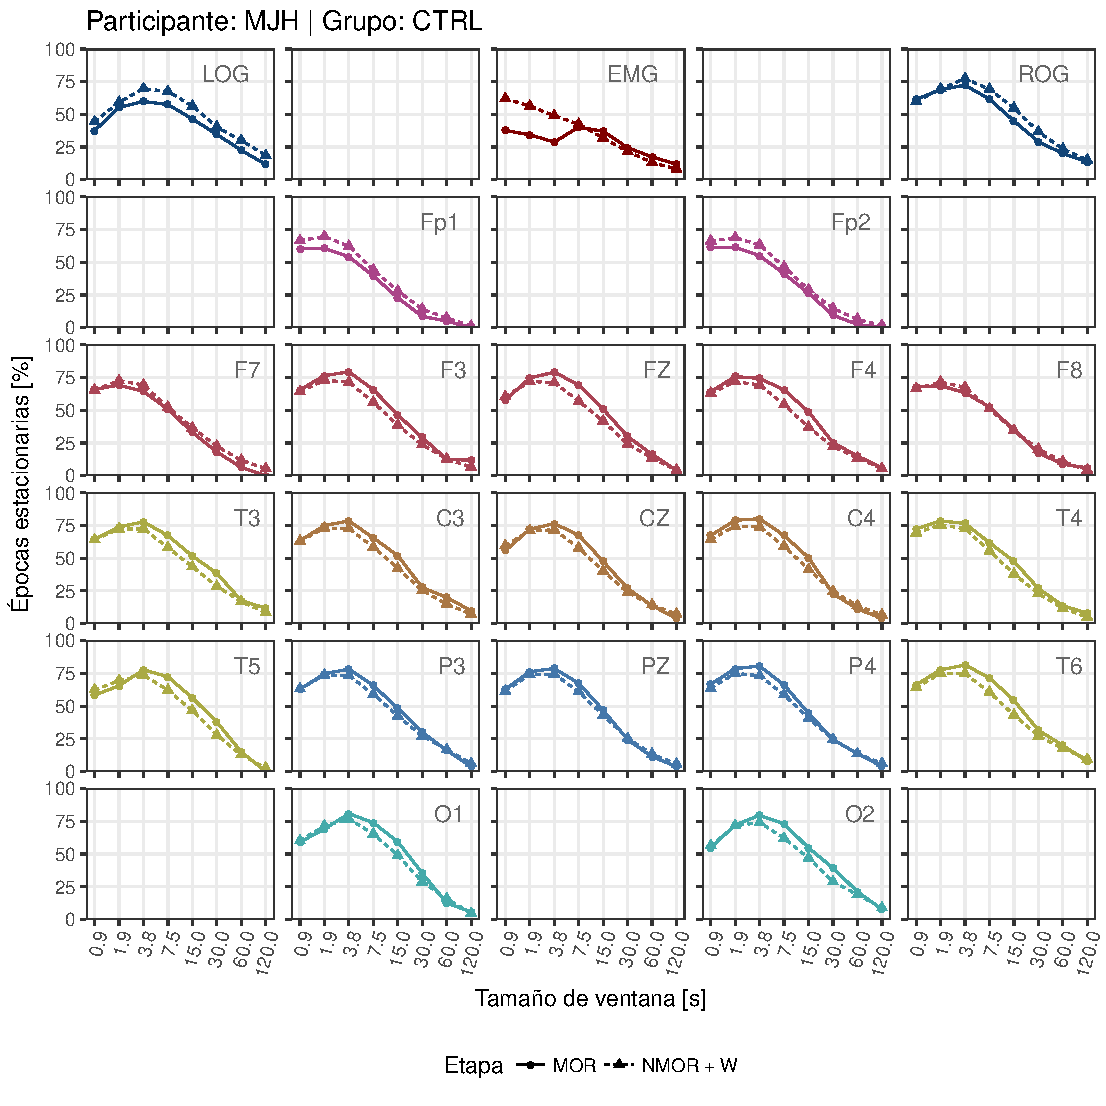
\includegraphics[width=\linewidth]{./scripts_graf_res/MJNNVIGILOS_cabeza_epocas_v2.pdf}
\caption{Cambio en la proporción de épocas estacionarias respecto al tamaño de ventana usado, durante MOR y NMOR. El análisis se repite en todas las derivaciones consideradas; la posición y color de cada gráfico se corresponden a aquellos de la figura \ref{img:estampa}. Sea abrevia W = vigilia, recordando que la cantidad tiempo de los registros clasificada como vigilia es negligible.}
\end{figure}

\begin{figure}
\centering
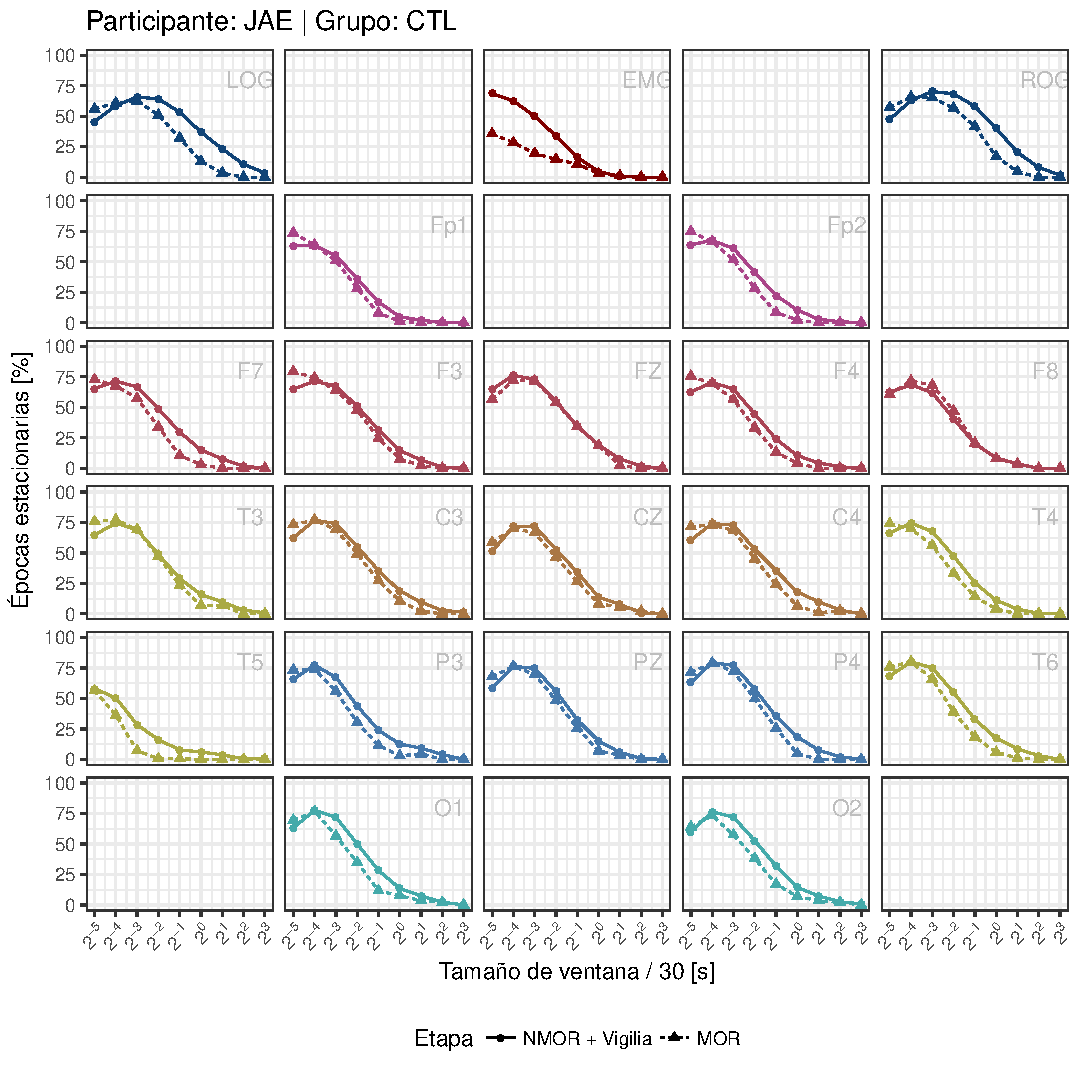
\includegraphics[width=\linewidth]{./scripts_graf_res/JANASUE_cabeza_epocas_v2.pdf}
\caption{Cambio en la proporción de épocas estacionarias respecto al tamaño de ventana usado, durante MOR y NMOR. El análisis se repite en todas las derivaciones consideradas; la posición y color de cada gráfico se corresponden a aquellos de la figura \ref{img:estampa}. Sea abrevia W = vigilia, recordando que la cantidad tiempo de los registros clasificada como vigilia es negligible.}
\end{figure}

\begin{figure}
\centering
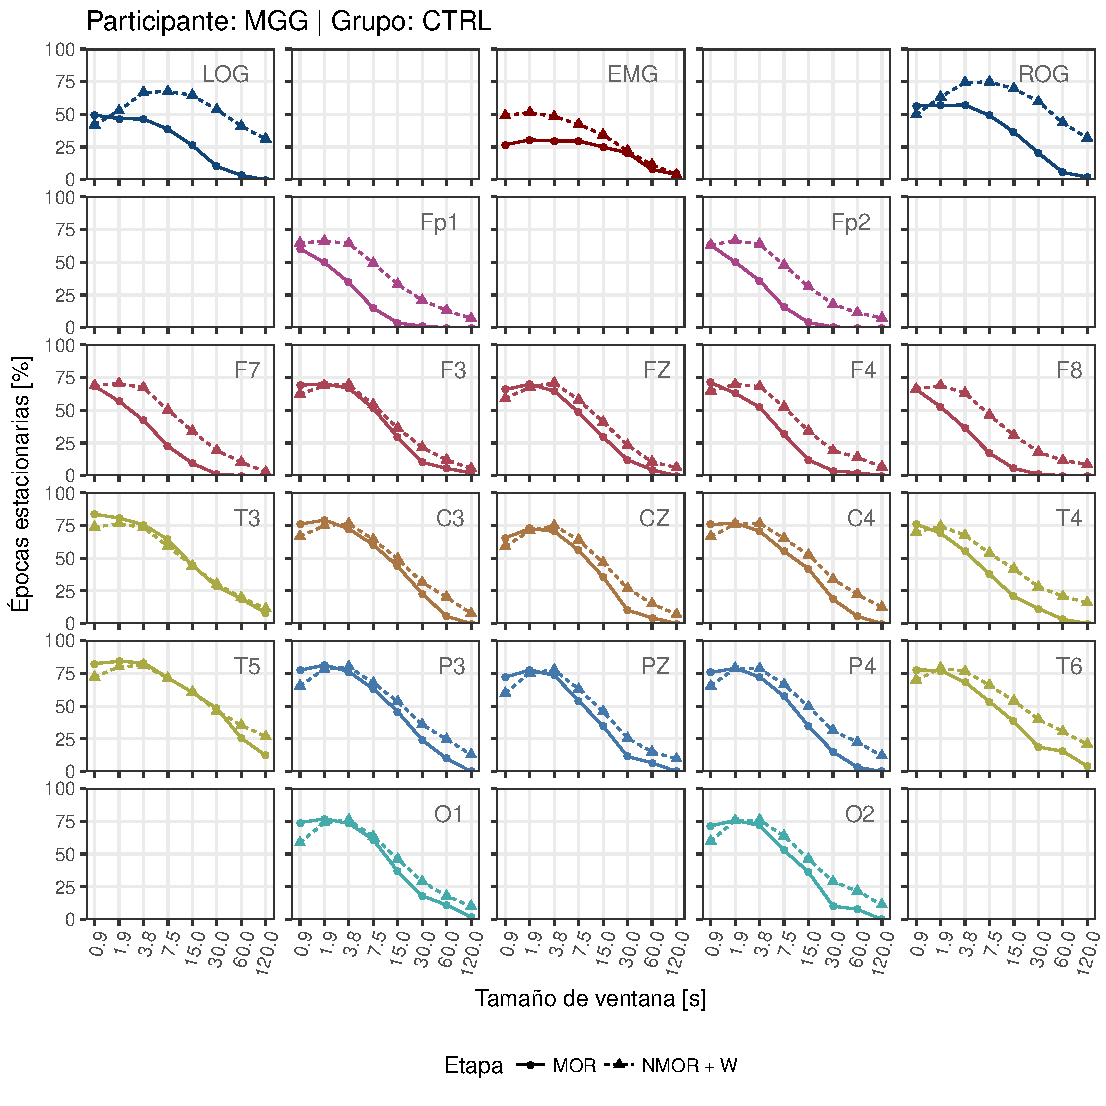
\includegraphics[width=\linewidth]{./scripts_graf_res/MGNA5SUE_cabeza_epocas_v2.pdf}
\caption{Cambio en la proporción de épocas estacionarias respecto al tamaño de ventana usado, durante MOR y NMOR. El análisis se repite en todas las derivaciones consideradas; la posición y color de cada gráfico se corresponden a aquellos de la figura \ref{img:estampa}. Sea abrevia W = vigilia, recordando que la cantidad tiempo de los registros clasificada como vigilia es negligible.}
\end{figure}

\begin{figure}
\centering
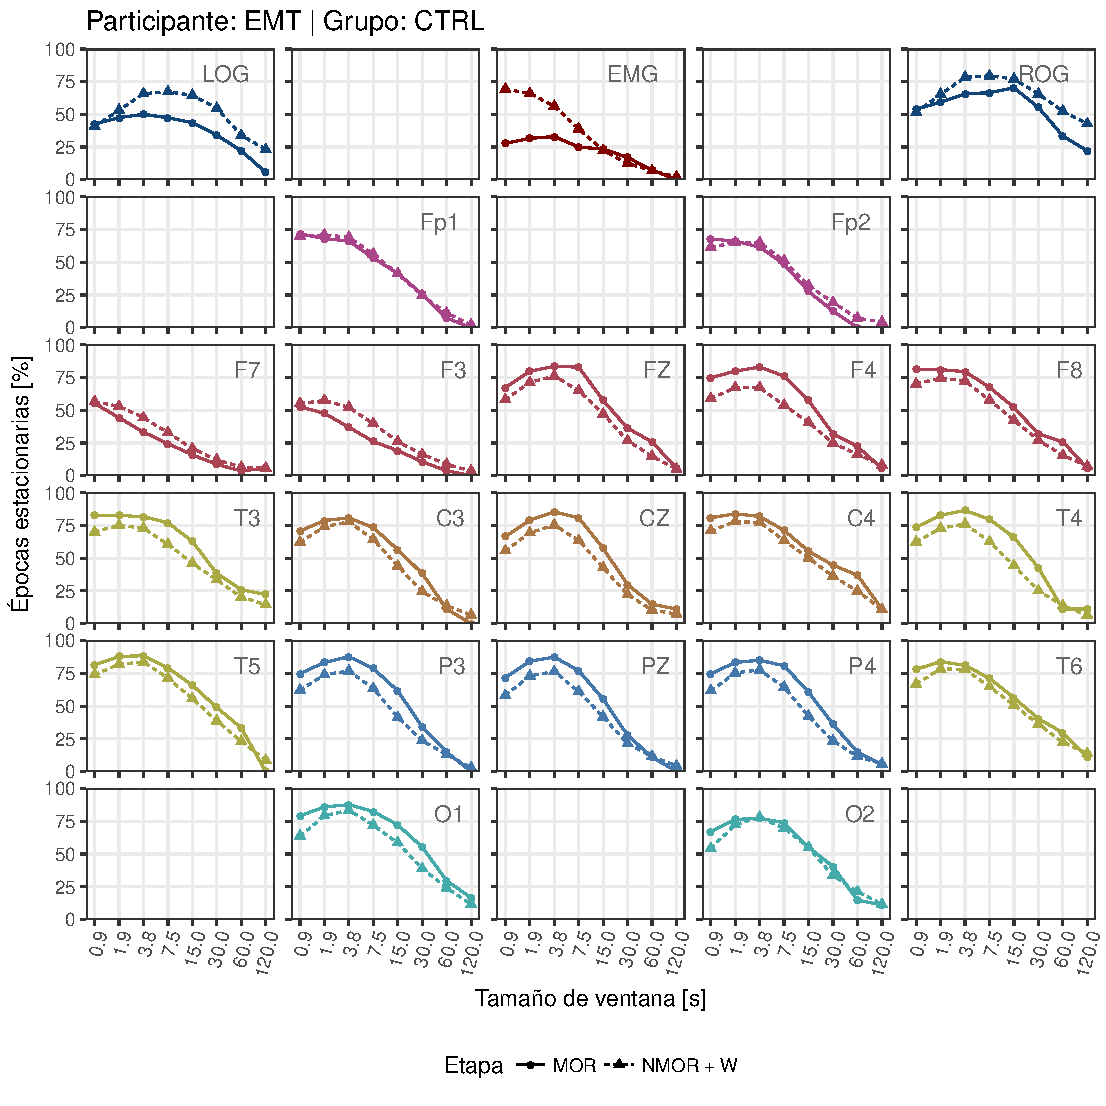
\includegraphics[width=\linewidth]{./scripts_graf_res/EMNNS_cabeza_epocas_v2.pdf}
\caption{Cambio en la proporción de épocas estacionarias respecto al tamaño de ventana usado, durante MOR y NMOR. El análisis se repite en todas las derivaciones consideradas; la posición y color de cada gráfico se corresponden a aquellos de la figura \ref{img:estampa}. Sea abrevia W = vigilia, recordando que la cantidad tiempo de los registros clasificada como vigilia es negligible.}
\end{figure}

\begin{figure}
\centering
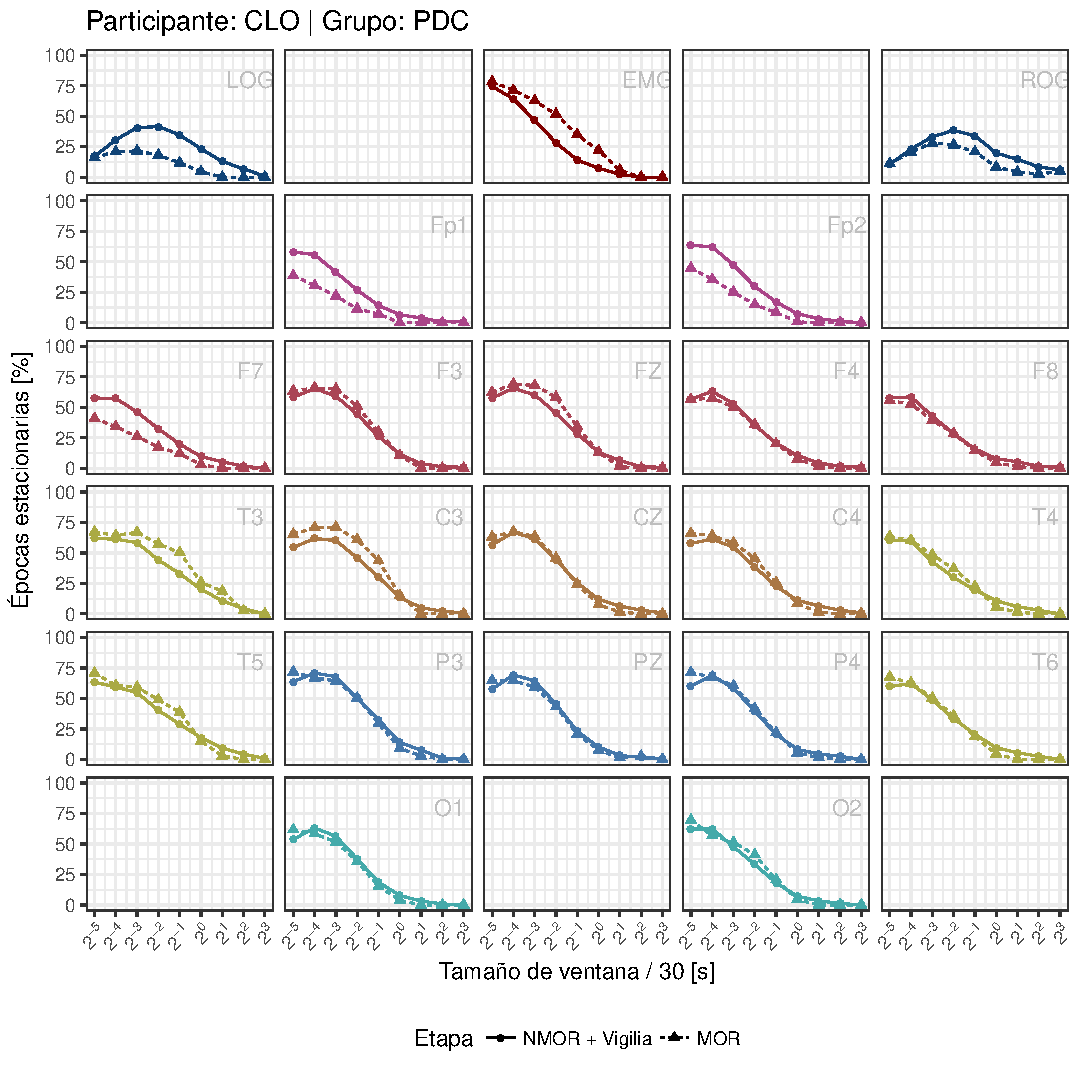
\includegraphics[width=\linewidth]{./scripts_graf_res/CLMN10SUE_cabeza_epocas_v2.pdf}
\caption{Cambio en la proporción de épocas estacionarias respecto al tamaño de ventana usado, durante MOR y NMOR. El análisis se repite en todas las derivaciones consideradas; la posición y color de cada gráfico se corresponden a aquellos de la figura \ref{img:estampa}. Sea abrevia W = vigilia, recordando que la cantidad tiempo de los registros clasificada como vigilia es negligible.}
\end{figure}

\begin{figure}
\centering
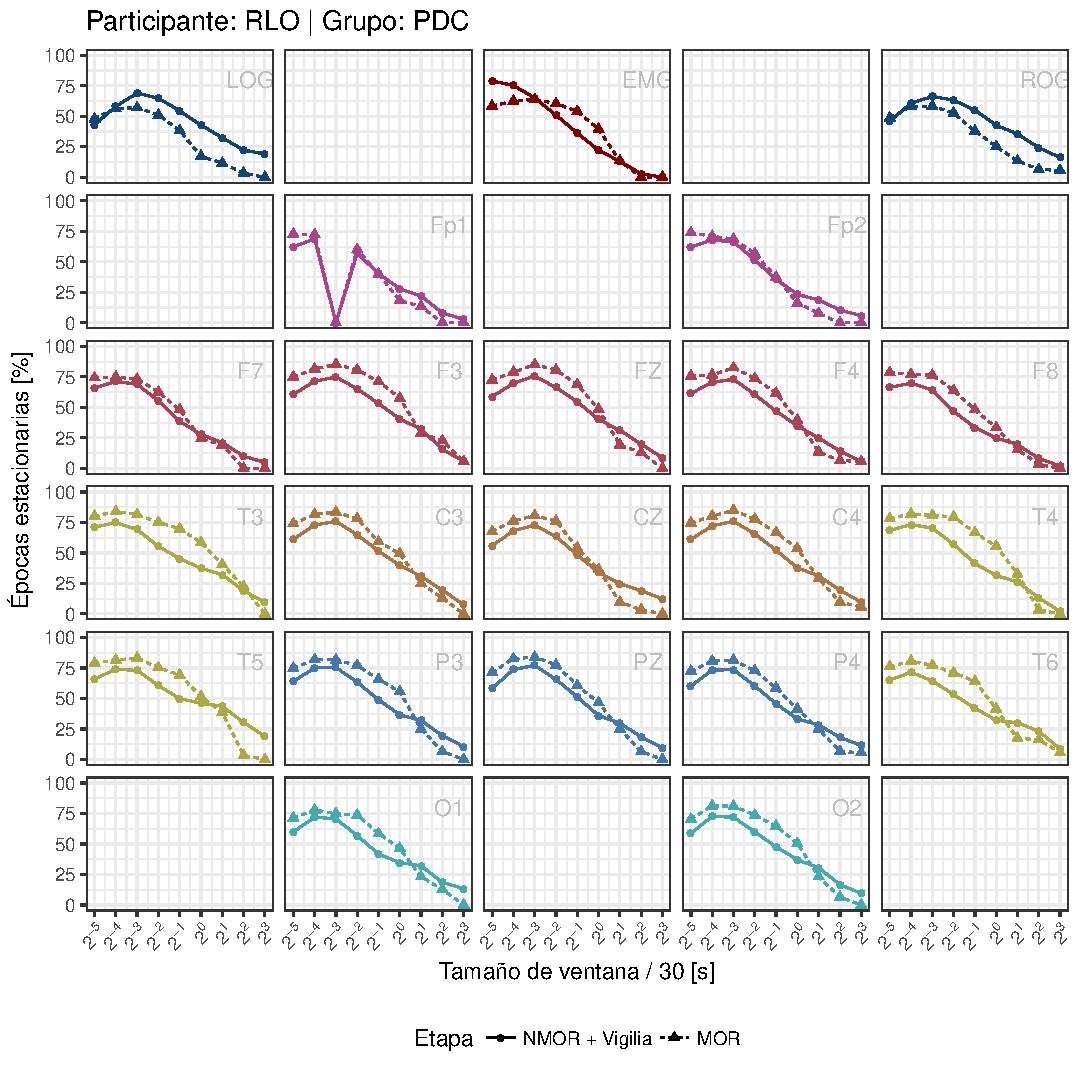
\includegraphics[width=\linewidth]{./scripts_graf_res/RLMN10SUE_cabeza_epocas_v2.pdf}
\caption{Cambio en la proporción de épocas estacionarias respecto al tamaño de ventana usado, durante MOR y NMOR. El análisis se repite en todas las derivaciones consideradas; la posición y color de cada gráfico se corresponden a aquellos de la figura \ref{img:estampa}. Sea abrevia W = vigilia, recordando que la cantidad tiempo de los registros clasificada como vigilia es negligible.}
\end{figure}

\begin{figure}
\centering
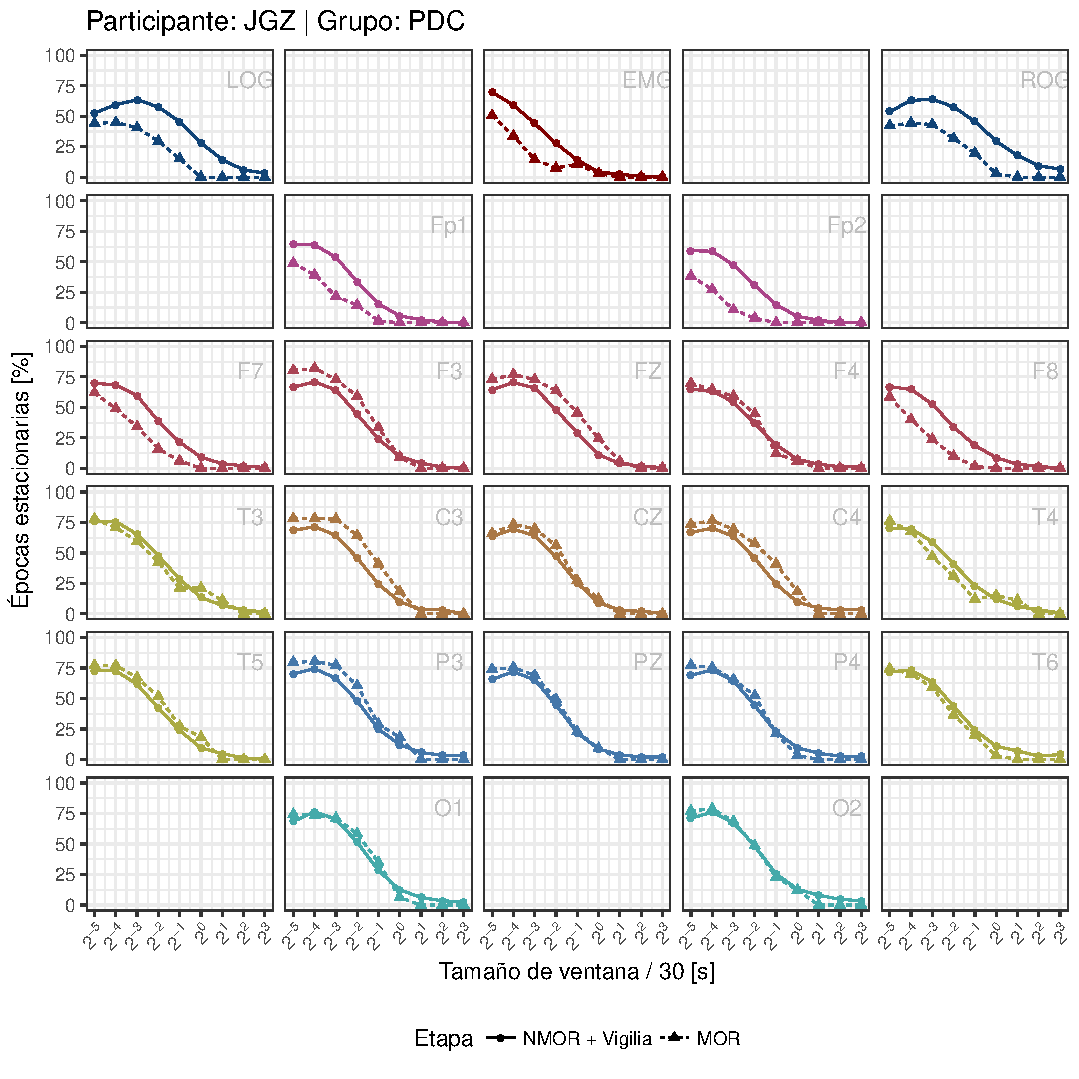
\includegraphics[width=\linewidth]{./scripts_graf_res/JGMN6SUE_cabeza_epocas_v2.pdf}
\caption{Cambio en la proporción de épocas estacionarias respecto al tamaño de ventana usado, durante MOR y NMOR. El análisis se repite en todas las derivaciones consideradas; la posición y color de cada gráfico se corresponden a aquellos de la figura \ref{img:estampa}. Sea abrevia W = vigilia, recordando que la cantidad tiempo de los registros clasificada como vigilia es negligible.}
\end{figure}

\begin{figure}
\centering
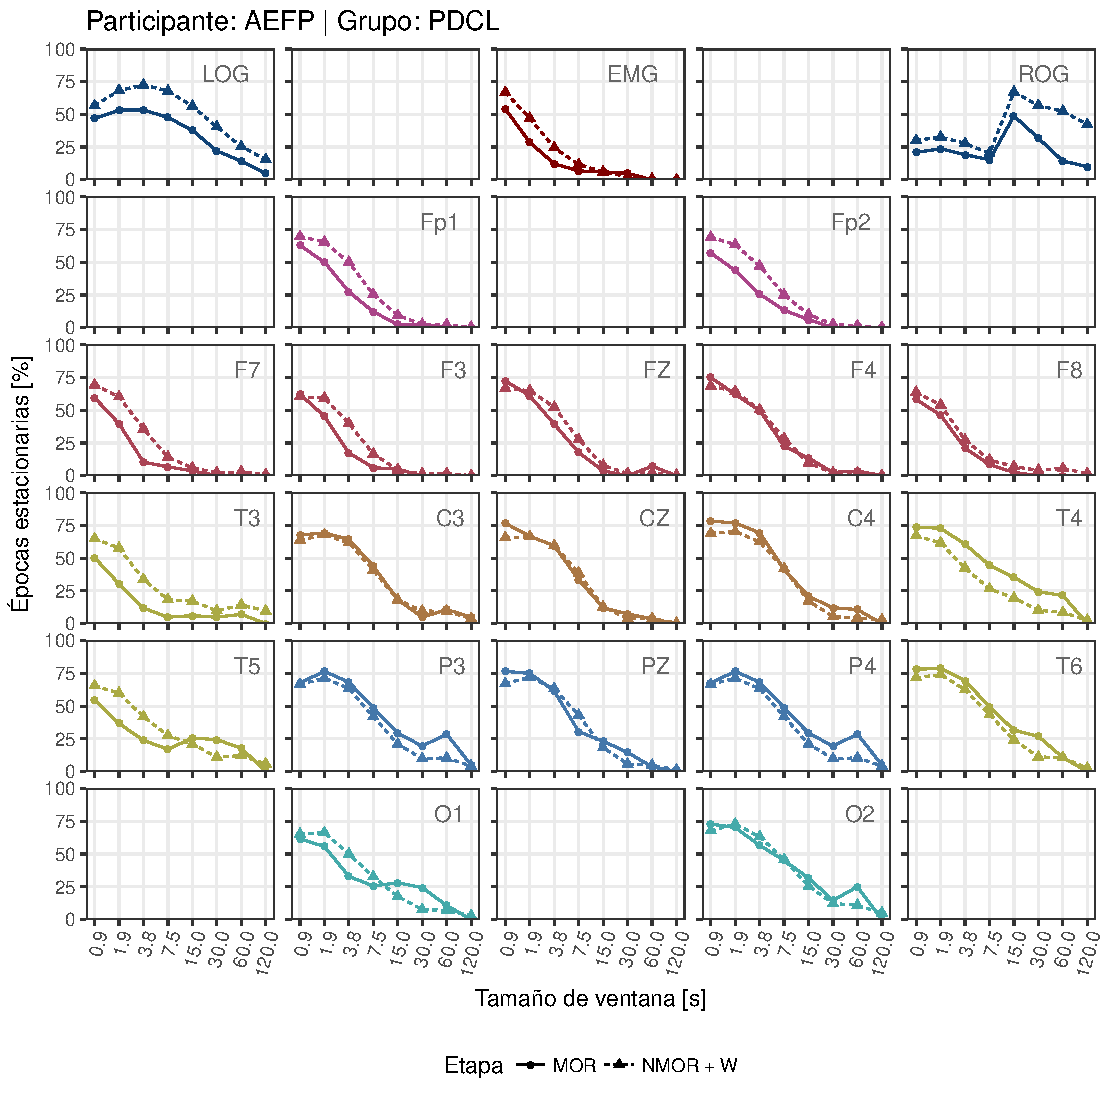
\includegraphics[width=\linewidth]{./scripts_graf_res/AEFP430714SUE_cabeza_epocas_v2.pdf}
\caption{Cambio en la proporción de épocas estacionarias respecto al tamaño de ventana usado, durante MOR y NMOR. El análisis se repite en todas las derivaciones consideradas; la posición y color de cada gráfico se corresponden a aquellos de la figura \ref{img:estampa}. Sea abrevia W = vigilia, recordando que la cantidad tiempo de los registros clasificada como vigilia es negligible.}
\end{figure}

\begin{figure}
\centering
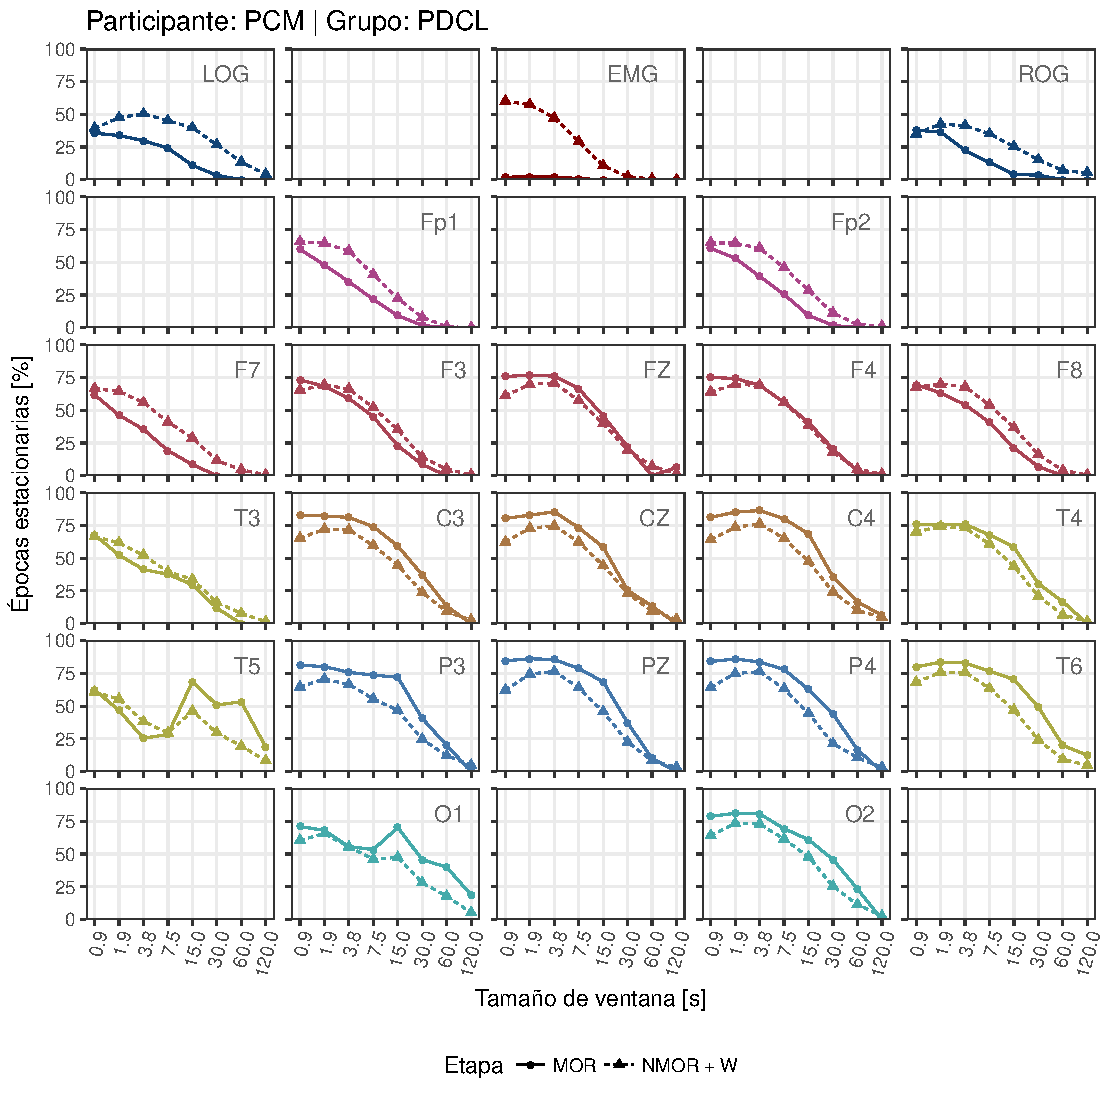
\includegraphics[width=\linewidth]{./scripts_graf_res/PCM90SUE_cabeza_epocas_v2.pdf}
\caption{Cambio en la proporción de épocas estacionarias respecto al tamaño de ventana usado, durante MOR y NMOR. El análisis se repite en todas las derivaciones consideradas; la posición y color de cada gráfico se corresponden a aquellos de la figura \ref{img:estampa}. Sea abrevia W = vigilia, recordando que la cantidad tiempo de los registros clasificada como vigilia es negligible.}
\end{figure}

%%%%%%%%%%%%%%%%%%%%%%%%%%%%%%%%%%%%%%%%%%%%%%%%%%%%%%%%%%%%%%%%%%%%%%%%%%%%%%%%%%%%%%%%%%%%%%%%%%%
%%%%%%%%%%%%%%%%%%%%%%%%%%%%%%%%%%%%%%%%%%%%%%%%%%%%%%%%%%%%%%%%%%%%%%%%%%%%%%%%%%%%%%%%%%%%%%%%%%%
%%%%%%%%%%%%%%%%%%%%%%%%%%%%%%%%%%%%%%%%%%%%%%%%%%%%%%%%%%%%%%%%%%%%%%%%%%%%%%%%%%%%%%%%%%%%%%%%%%%

%\input{tablas_skip.tex}

%%%%%%%%%%%%%%%%%%%%%%%%%%%%%%%%%%%%%%%%%%%%%%%%%%%%%%%%%%%%%%%%%%%%%%%%%%%%%%%%%%%%%%%%%%%%%%%%%%%%
%%%%%%%%%%%%%%%%%%%%%%%%%%%%%%%%%%%%%%%%%%%%%%%%%%%%%%%%%%%%%%%%%%%%%%%%%%%%%%%%%%%%%%%%%%%%%%%%%%%%
%%%%%%%%%%%%%%%%%%%%%%%%%%%%%%%%%%%%%%%%%%%%%%%%%%%%%%%%%%%%%%%%%%%%%%%%%%%%%%%%%%%%%%%%%%%%%%%%%%%%
%%%%%%%%%%%%%%%%%%%%%%%%%%%%%%%%%%%%%%%%%%%%%%%%%%%%%%%%%%%%%%%%%%%%%%%%%%%%%%%%%%%%%%%%%%%%%%%%%%%%

\pagestyle{plain}

\bibliographystyle{bababbrv-lf}
\bibliography{referencias_todo}%{}

%%%%%%%%%%%%%%%%%%%%%%%%%%%%%%%%%%%%%%%%%%%%%%%%%%%%%%%%%%%%%%%%%%%%%%%%%%%%%%%%%%%%%%%%%%%%%%%%%%%
%%%%%%%%%%%%%%%%%%%%%%%%%%%%%%%%%%%%%%%%%%%%%%%%%%%%%%%%%%%%%%%%%%%%%%%%%%%%%%%%%%%%%%%%%%%%%%%%%%%

\end{document}

%%%%%%%%%%%%%%%%%%%%%%%%%%%%%%%%%%%%%%%%%%%%%%%%%%%%%%%%%%%%%%%%%%%%%%%%%%%%%%%%%%%%%%%%%%%%%%%%%%%
%%%%%%%%%%%%%%%%%%%%%%%%%%%%%%%%%%%%%%%%%%%%%%%%%%%%%%%%%%%%%%%%%%%%%%%%%%%%%%%%%%%%%%%%%%%%%%%%%%%
%%%%%%%%%%%%%%%%%%%%%%%%%%%%%%%%%%%%%%%%%%%%%%%%%%%%%%%%%%%%%%%%%%%%%%%%%%%%%%%%%%%%%%%%%%%%%%%%%%%
%%%%%%%%%%%%%%%%%%%%%%%%%%%%%%%%%%%%%%%%%%%%%%%%%%%%%%%%%%%%%%%%%%%%%%%%%%%%%%%%%%%%%%%%%%%%%%%%%%%

@Article{rosales2017stationarity,
    title   = {Stationarity {D}uring {REM} {S}leep in {O}ld {A}dults},
    author  = {Rosales-Lagarde, Alejandra 
               and Rodr{\'\i}guez-Torres, Erika 
               and Enciso-Alva, Julio 
               and Mart{\'\i}nez-Alcal{\'a}, Claudia 
               and V{\'a}zquez-Tagle, G{\'e}nesis 
               and Tetlalmatzi-Montiel, Margarita 
               and Viveros, Jorge 
               and L{\'o}pez-Noguerola, Jos{\'e} S{\'o}crates},
    journal = {{Alzheimer's \& Dementia: The Journal of the Alzheimer's Association}},
    volume  = {13},
    number  = {7},
    pages   = {P723--P724},
    year    = {2017},
    publisher={Elsevier}
}
